% !TeX spellcheck = en_GB
%%%%%%%%%%%%%%%%%%%%%%%%%%%%%%%%%%%%%%%%%%
%                                        %
%    Engineer thesis LaTeX template      %
%  compliant with the SZJK regulations   %
%                                        %
%%%%%%%%%%%%%%%%%%%%%%%%%%%%%%%%%%%%%%%%%%
%                                        %
%  (c) Krzysztof Simiński, 2018-2024     %
%                                        %
%%%%%%%%%%%%%%%%%%%%%%%%%%%%%%%%%%%%%%%%%%
%                                        %
% The latest version of the templates is %
% available at                           %
% github.com/ksiminski/polsl-aei-theses  %
%                                        %
%%%%%%%%%%%%%%%%%%%%%%%%%%%%%%%%%%%%%%%%%%
%
%
% This LaTeX project formats the final thesis
% with compliance to the SZJK regulations.
% Please to not change formatting (fonts, margins,
% bolds, italics, etc).
%
% You can compile the project in several ways.
%
% 1. pdfLaTeX compilation
%
% pdflatex main
% bibtex   main
% pdflatex main
% pdflatex main
%
%
% 2. XeLaTeX compilation
%
% Compilation with the XeLaTeX engine inserts Calibri font
% in the title page. Of course the font has to be installed.
%

% xelatex main
% bibtex  main
% xelatex main
% xelatex main
%
%
%%%%%%%%%%%%%%%%%%%%%%%%%%%%%%%%%%%%%%%%%%%%%%%%%%%%%%%%%%%%%%
% If you have any questions, remarks, just send me an email: %
%            krzysztof.siminski(at)polsl.pl               %
%%%%%%%%%%%%%%%%%%%%%%%%%%%%%%%%%%%%%%%%%%%%%%%%%%%%%%%%%%%%%%

% We would like to improve the LaTeX templates
% of final theses. By answering the questions
% in the survey whose address your can find below
% you help us to do so. The survey is completely
% anonimous. Thank you!
%
% https://docs.google.com/forms/d/e/1FAIpQLScyllVxNKzKFHfILDfdbwC-jvT8YL0RSTFs-s27UGw9CKn-fQ/viewform?usp=sf_link
%
%%%%%%%%%%%%%%%%%%%%%%%%%%%%%%%%%%%%%%%%%%%%%%%%%%%%%%%%%%%%%%%%%%%%%%%%%

%%%%%%%%%%%%%%%%%%%%%%%%%%%%%%%%%%%%%%%%%%%%%%%
%                                             %
% CUSTOMISATION OF THE THESIS                 %
%                                             %
%%%%%%%%%%%%%%%%%%%%%%%%%%%%%%%%%%%%%%%%%%%%%%%

% Please customise your thesis with the macros below.

% TODO
% author:
\newcommand{\FirstNameAuthor}{Michał Dominik}
\newcommand{\SurnameAuthor}{Rajzer}
\newcommand{\IdAuthor}{306081}  % (remove  and 

% coauthor:
%\newcommand{\FirstNameCoauthor}{First Names}  % If there is a coauthor, put the first names here.
%\newcommand{\SurnameCoauthor}{Surname}        % If there is a coauthor, put the surnames here.
%\newcommand{\IdCoauthor}{student id} % If there is a coauthor, put the student id here (remove  and 
% If there is no coathor, leave the definitions empty like below. If a coauthor exists, comment the lines below.
\newcommand{\FirstNameCoauthor}{Jakub} % If there is only one author, leave the definitions empty.
\newcommand{\SurnameCoauthor}{Sanecki}   % If there is only one author, leave the definitions empty.
\newcommand{\IdCoauthor}{306085}        % If there is only one author, leave the definitions empty.
%%%%%%%%%%

\newcommand{\Supervisor}{Jakub Nalepa, PhD, DSc}  % supervisor (remove  and 
\newcommand{\Title}{Where deep learning meets Earth observation satellites: Compression and analysis of hyperspectral images}
\newcommand{\TitleAlt}{Gdzie uczenie głębokie spotyka się z satelitami obserwacji Ziemi: kompresja i analiza obrazów hiperspektralnych}
\newcommand{\Program}{Informatics}
\newcommand{\Specialisation}{Computer Graphics and Software} % your specialisation (remove  and , I'm 98% sure that this is the name of the specialisation TODO: make sure
\newcommand{\Departament}{of Algorithmics and Software} % your supervisor's departament (remove  and 


% If you have a consultant for your thesis, put their name below ...
\newcommand{\Consultant}{}  %  (remove  and 
% ... else leave the braces empty:
%\newcommand{\Consultant}{} % no consultant

% end of thesis customisation
%%%%%%%%%%%%%%%%%%%%%%%%%%%%%%%%%%%%%%%%%%

%%%%%%%%%%%%%%%%%%%%%%%%%%%%%%%%%%%%%%%%%%%%%%%
%                                             %
% END OF CUSTOMISATION                        %
%                                             %
%%%%%%%%%%%%%%%%%%%%%%%%%%%%%%%%%%%%%%%%%%%%%%%

%%%%%%%%%%%%%%%%%%%%%%%%%%%%%%%%%%%%%%%%

\input{config/settings.tex} % Do not modify!


%%%%%%%%%%%%%%%%%%%%%%%%%%%%%%%%%%%%%%%%%%%%%%%
%                                             %
% MY PACKAGES, SETTINGS ETC.                  %
%                                             %
%%%%%%%%%%%%%%%%%%%%%%%%%%%%%%%%%%%%%%%%%%%%%%%

% Put your packages, macros, setting here.




%%%%%%%%%%%%%%%%%%%%%%%%%%%%%%%%%%%%%%%%%%%%%%%%%%%%%%%%%%%%%%%%%%%%%
% listings
% packages: listings or minted
% % % % % % % % % % % % % % % % % % % % % % % % % % % % % % % % % % % 

\setcounter{biburllcpenalty}{7000}  % Allow URL breaks at lowercase letters
\setcounter{biburlucpenalty}{8000}  % Allow URL breaks at uppercase letters

% package listings

\usepackage{pgfplots}
\pgfplotsset{compat=1.18}

\pgfplotsset{
    colormap={blueblackred}{
        rgb255(0cm)=(0,0,255);     % blue
        rgb255(1cm)=(0,0,0);       % black
        rgb255(2cm)=(255,0,0);     % red
    }
}

\usepackage{graphicx}
\usepackage{listings}
\lstset{%
    morekeywords={string,exception,std,vector},% add the keyword you need
    language=C++,% C, Matlab, Python, SQL, TeX, XML, bash, ... – vide https://www.ctan.org/pkg/listings
    commentstyle=\textit,%
    identifierstyle=\textsf,%
    keywordstyle=\sffamily\bfseries, %\texttt, %
    %captionpos=b,%
    tabsize=3,%
    frame=lines,%
    numbers=left,%
    numberstyle=\tiny,%
    numbersep=5pt,%
    breaklines=true,%
    escapeinside={@*}{*@},%
}
\usepackage{caption}

\usepackage{tikz}
\usepackage[edges]{forest}
\usepackage{enumitem}
\newlist{speclist}{itemize}{1}
\setlist[speclist]{
    label=\textbullet,
    leftmargin=2em,
    itemsep=1pt,
    parsep=0pt,
    topsep=2pt,
    partopsep=0pt
}
\usepackage{array}
\usepackage{multirow}  % for \multirow command in tables
\usepackage{threeparttable}  % for tablenotes environment
% % % % % % % % % % % % % % % % % % % % % % % % % % % % % % % % % % % 
% package minted
\usepackage{minted}

% This package requires a special command line option in compilation
% pdflatex -shell-escape main.tex
% xelatex  -shell-escape main.tex

% \usepackage[chapter]{minted} % [section]
\usemintedstyle{bw}   % black and white codes

\setminted % https://ctan.org/pkg/minted
{
    %fontsize=\normalsize,%\footnotesize,
    %captionpos=b,%
    tabsize=3,%
    frame=lines,%
    framesep=2mm,
    numbers=left,%
    numbersep=5pt,%
    breaklines=true,%
    escapeinside=@@,%
}

%%%%%%%%%%%%%%%%%%%%%%%%%%%%%%%%%%%%%%%%%%%%%%%%%%%%%%%%%%%%%%%%%%%%%

\usepackage{tikz}
\usetikzlibrary{arrows,positioning}

%%%%%%%%%%%%%%%%%%%%%%%%%%%%%


%%%%%%%%%%%%%%%%%%%%%%%%%%%%%%%%%%%%%%%%%%%%%%%
%                                             %
% END OF MY PACKAGES, SETTINGS ETC.           %
%                                             %
%%%%%%%%%%%%%%%%%%%%%%%%%%%%%%%%%%%%%%%%%%%%%%%

 % Put your settings, packages, macros here.

%%%%%%%%%%%%%%%%%%%%%%%%%%%%%%%%%%%%%%%%


\begin{document}
%\kslistofremarks

\frontmatter
\input{config/titlepage.tex}  % Please to not modify the titlepage.tex file!

\cleardoublepage

\rmfamily\normalfont
\pagestyle{empty}


%%% Let's start the thesis %%%%

% TODO
\subsubsection*{Thesis title}
\Title

\subsubsection*{Abstract}
    Hyperspectral images (HSIs) provide detailed spectral information across hundreds of bands but generate significantly larger data volumes than traditional RGB images, creating challenges for storage and transmission in resource-constrained environments such as satellites. 
    This thesis explores deep learning-based compression methods for HSIs, implementing and evaluating four models: LineRWKV for lossless compression, and RCAE2D1D, RCAE3D, and RCGDNAE for lossy compression.
    The models were trained and tested on the HySpecNet11k dataset, with performance assessed using metrics such as Bits Per Pixel Per Band (BPPPB), Peak Signal-to-Noise Ratio (PSNR), and Structural Similarity Index Measure (SSIM).
    Another important aspect of this work is the evaluation of the feasibility of these models for downstream tasks, specifically semantic segmentation, which was assessed using a separate model trained on the original, uncompressed data.
    The results indicate that deep learning-based compression techniques can effectively reduce HSI data sizes while maintaining differing quality for both visual assessment and semantic segmentation tasks depending on the model with some models excelling in visual quality and others in segmentation performance.

\subsubsection*{Key words}
Deep Learning, Compression, Hyperspectral Images

\subsubsection*{Tytuł pracy}
\begin{otherlanguage}{polish}
    \TitleAlt
\end{otherlanguage}

\subsubsection*{Streszczenie}
\begin{otherlanguage}{polish}
    Obrazy hiperspektralne (HSI) dostarczają szczegółowych informacji spektralnych w setkach pasm, ale generują znacznie większe wolumeny danych niż tradycyjne obrazy RGB, co stwarza wyzwania związane z przechowywaniem i transmisją w środowiskach o ograniczonych zasobach, takich jak satelity.
    Niniejsza praca bada metody kompresji oparte na uczeniu głębokim dla HSI, implementując i oceniając cztery modele: LineRWKV do kompresji bezstratnej oraz RCAE2D1D, RCAE3D i RCGDNAE do kompresji stratnej.
    Modele zostały wytrenowane i przetestowane na zbiorze danych HySpecNet11k, a wydajność oceniono za pomocą metryk takich jak bity na piksel na pasmo (BPPPB), szczytowy stosunek sygnału do szumu (PSNR) oraz wskaźnik podobieństwa strukturalnego (SSIM).
    Kolejnym ważnym aspektem tej pracy jest ocena wykonalności tych modeli dla zadań następczych, w szczególności segmentacji semantycznej, która została oceniona za pomocą oddzielnego modelu wytrenowanego na oryginalnych, nieskompresowanych danych.
    Wyniki wskazują, że techniki kompresji oparte na uczeniu głębokim mogą skutecznie zmniejszyć rozmiary danych HSI, zachowując różną jakość zarówno do oceny wizualnej, jak i zadań segmentacji semantycznej w zależności od modelu, przy czym niektóre modele wyróżniają się jakością wizualną, a inne wydajnością segmentacji.

\end{otherlanguage}

\subsubsection*{Słowa kluczowe}
\begin{otherlanguage}{polish}
    Uczenie Głębokie, Kompresja, Obrazy Hiperspektralne
\end{otherlanguage}

 % editorials


%%%%%%%%%%%%%%%%%% Table of contents %%%%%%%%%%%%%%%%%%%%%%
% Add \thispagestyle{empty} to the toc file (main.toc), because \pagestyle{empty} doesn't work if the TOC has multiple pages
\addtocontents{toc}{\protect\thispagestyle{empty}}
\tableofcontents

%%%%%%%%%%%%%%%%%%%%%%%%%%%%%%%%%%%%%%%%%%%%%%%%%%%%%
\setcounter{pagesWithoutNumbers}{\value{page}}
\mainmatter
\pagestyle{empty}

\cleardoublepage

\pagestyle{PageNumbersChapterTitles}

%%%%%%%%%%%%%% body of the thesis %%%%%%%%%%%%%%%%%

% TODO
\chapter{Introduction}

% \begin{itemize}
%     \item introduction into the problem domain
%     \item settling of the problem in the domain
%     \item objective of the thesis
%     \item scope of the thesis
%     \item short description of chapters
%     \item clear description of contribution of the thesis's author – in case of more authors table with enumeration of contribution of authors
% \end{itemize}
\section{Introduction, thesis goal}
Earth observation began as an exclusively scientific endeavor and has developed into an essential service aimed at the observation, interpretation, and management of the various Earth systems.
The widespread use of satellites and other remote earth observation platforms results in the generation of a massive amount of data daily.
This data is the backbone of various applications including agriculture~~\cite{chemometrics_environmental_monitoring2020}, forestry~~\cite{remote_sensing_uav_hyperspectral2017}, surveillance~~\cite{HSI_security_surveillance2010}, geology~~\cite{geology2012} and environmental monitoring~~\cite{environmental_monitoring_hyperspectral2009}.\par
%
Traditionally, a vast majority of the optical data has been acquired by panchromatic or multispectral cameras.
Of these, the most common type of camera is the RGB (Red, Green, Blue), which mimic human eye by capturing data in three primary color channels: red (635 nm--700 nm), green (490 nm--560 nm), and blue (450 nm--490 nm) ~\cite{ColorWavelengths2014}.
Although RGB images provide enough information for visual analysis and simple categorizations, they lack the depth of information required for more advanced applications.\par
%
This limitation has driven the development and deployment of hyperspectral imaging sensors (HSIS).
Unlike their traditional counterparts, HSIS behave like an optical spectrometer on a per-pixel basis.
HSIs go beyond three bands by providing data across dozens or even hundreds of very narrow spectral bands, which may include wavelengths outside the visible spectrum — from the ultraviolet (UV) and visible to the near-infrared (NIR) and short-wave infrared (SWIR) regions, typically ranging from 400 nm to 2.5 $\mu$m, with each band only a few nanometers wide ~\cite{lossless_comprehensive_review2025}.
The resulting dataset is a three-dimensional data cube that contains two dimensions of spatial information (x, y) and one dimension of spectral information ($\lambda$),
which contains a distinct spectral signature or ``fingerprint'' for each imaged material.
These signatures enable the differentiation of materials and objects that cannot be distinguished from each other in conventional images ~\cite{geology2012}.\par
%
The use that can be made with this level of spectral detail is unparalleled.
In agriculture applications, the use of HSIs helps to monitor nutrient deficiencies and diseases before they become visible to the naked eye~\cite{chemometrics_environmental_monitoring2020}.
In the management of forest resources, HSIs help to assess species distribution, weight, and pest infestations ~\cite{remote_sensing_uav_hyperspectral2017}.
Geology applications include mineral mapping and soil composition analysis ~\cite{geology2012}.
Additionally, HSIs play critical roles in surveillance and environmental applications by enabling the detection of camouflaged objects and monitoring of pollution levels ~\cite{HSI_security_surveillance2010, environmental_monitoring_hyperspectral2009}.
Most uses directly involve the analysis of the spectral signatures present in the data, allowing for more accurate and detailed assessments than traditional imaging methods.
A common technique used in HSI analysis is semantic segmentation, where each pixel in the image is classified into different categories based on its spectral signature ~\cite{magic}.\par
%
However, the informational density of HSIs comes at a cost.
A single HSI pixel no longer contains three values, but a vector of hundreds ~\cite{remote_sensing_uav_hyperspectral2017}.
This results in significantly larger data sizes compared to traditional images, posing challenges for storage, transmission, and processing, especially in resource-constrained environments like satellites.
To mitigate these challenges, effective compression techniques are essential.
Over the years, a variety of compression methods have been proposed, ranging from adaptations of traditional compression algorithms to deep learning-based approaches specifically designed for HSI ~\cite{lossless_comprehensive_review2025}.\par
%
In this thesis, the focus is placed on the exploration and evaluation of selected HSI compression methods based on deep learning, which already exist in the literature.
The goal is to compare these methods in terms of Compression Ratio (CR), reconstruction quality, and computational requirements for both lossy and lossless compression.
Another goal is to check the feasibility of these methods by including a simple semantic segmentation model in the evaluation pipeline to assess the impact of compression on downstream tasks.
To achieve this, a custom data pipeline was developed to facilitate the training and evaluation of the selected methods on a standard dataset ~\cite{HySpecNet11k}.
We divided the work so that one author focused on two lossy compression methods while the other focused on one lossless and one lossy compression method, and both authors collaborated on the data pipeline and the semantic segmentation model.

% Earth observation is becoming a vital tool in monitoring and understanding our planet.
% Satellites and aerial vehicles gather vast amounts of data, which can be used for various applications.
% Traditional imaging sensors capture data in three primary color channels: red (635nm-700nm), green (490nm-560nm), and blue (450nm-490nm)~\cite{ColorWavelengths2014}.
% Although, the need for more detailed and information-dense data has pushed past such simple systems towards hyperspectral imaging sensors (HSIS). HSIS go beyond three channels by capturing data across dozens or even hundreds of narrow spectral bands.\\

% These bands can range far beyond the range of typical RGB image sensors, from far infrared to deep UV or from 2.5$\mu$m to 400nm with each band being as narrow as several nm~\cite{lossless_comprehensive_review2025}.
% Such small bands allow for the detection of subtle differences in material properties that are not discernible with traditional imaging as well as they allow for the identification of materials based on their spectral signatures~\cite{}.
% This, in turn, makes these useful for many applications including agriculture~\cite{chemometrics_environmental_monitoring2020}, forestry~\cite{remote_sensing_uav_hyperspectral2017}, surveilance~\cite{HSI_security_surveillance2010}, geology~\cite{geology2012} and environmental monitoring~\cite{environmental_monitoring_hyperspectral2009}.\\

% However, the high spectral resolution of hyperspectral images (HSIs) comes at the cost of significantly higher sizes of the images.
% Each pixel in a HSI contains a full spectrum of data across many bands rather than just three color values.
% This in turn creates a problem for applications where HSIS are most in demand such as satellites which operate under strict constraints on onboard storage, memory, power consumption and communications bandwidth~\cite{}.
% Furtheremore, the downlink bandwidth from satellites to ground stations might not be available at all times which makes it necessary to store large amounts of data onboard for extended periods of time~\cite{}.
% To address these challenges, many different solutions were proposed over the years including traditional compression algorithms adapted for HSIs as well as novel methods based on deep learning~\cite{lossless_comprehensive_review2025}.\\
% In this thesis, the focus is placed on the exploration and evaluation of selected HSI compression methods based on deep learning which already exist in literature.
% The goal is to compare these methods in terms of compression ratio, reconstruction quality and computational requirements for both lossy and lossless compression.
% To achieve this, a custom data pipeline was developed to facilitate the training and evaluation of the selected methods on a standard dataset~\cite{HySpecNet11k}.
% We divided the work so that one author focuses on lossy compression methods while the other focuses on lossless compression methods.
% The contributions of the authors are summarized in Table \ref{tab:contribution}.
\section{Chapter overview}
The thesis is structured into several chapters. This section provides the structure of the thesis and a brief description of each chapter.
\begin{enumerate}
    \item {\bf Introduction} Introduces the topic of hyperspectral image compression, outlines the goals of the thesis, and summarizes the contributions of the authors.
    \item {\bf Literature} This chapter reviews existing literature on HSI compression, covering lossy and lossless methods, traditional and deep learning-based approaches, and relevant metrics for evaluating compression performance.
    \item {\bf Dataset} Description of the dataset used for training and testing the models, and a custom visualization tool developed to better understand the dataset.
    \item {\bf External specifications} Description of the tools and libraries used in the implementation of the models. Details instalation process and system requirements.
    \item {\bf Internal specifications} Description of the custom data pipeline developed for training and evaluation of the models. Details the architecture and functionality of the pipeline as well as its components and data structure.
    \item {\bf Machine learning model implementation} This chapter introduces the fundamental concepts of machine learning. It is focused on structures and the mathematics behind neural networks. It details activation functions and explains the use of optimizers.
    \item {\bf Lossless compression model: LineRWKV} In this chapter, the LineRWKV model for lossless compression is introduced. It details the model's structure, its implementation, and training process.
    \item {\bf Lossy compression model: Residual Convolutional Autoencoders} This chapter focuses on residual convolutional autoencoders for lossy compression. It presents the implementation and training results for two variants, a 3D RCAE and a hybrid 2D-1D RCAE.
    \item {\bf Lossy compression model: Reduced Complexity General Divisive Normalisation Autoencoder} This chapter presents the RCGDNAE, a lossy compression model for HSI, that enhances a standard autoencoder with fixed KLT preprocessing and GDN activation layers.
    \item {\bf Verification and validation} This chapter is focused on describing the methods and procedures used for verification and validation of the implemented models. It details the evaluation metrics used to assess the performance of the models.
    \item {\bf Conclusion} Chapter that summarizes the results of the presented compression models while acknowledging limitations and proposing future improvement.
\end{enumerate}

\section{Contribution of the authors}
Table \ref{tab:contribution} summarizes the contributions of each author to different parts of the thesis. It highlights the division of work between the authors in terms of chapters and specific topics covered.
\begin{table}[h!]
    \centering
    \caption{Summary of the contribution of the authors.}
    \label{tab:contribution}
    \begin{tabular}{m{20em}| m{10em}}
        \toprule
        Part of the thesis                                                                                & Author \\
        \midrule
        Chapter 1. Introduction                                                                           & MR, JS \\
        \hline
        Chapter 2. Literature                                                                             & MR, JS \\
        \hline
        Chapter 3. Dataset                                                                                & MR, JS \\
        \hline
        Chapter 4. External specifications                                                                & MR, JS \\
        \hline
        Chapter 5. Internal specifications                                                                & MR, JS \\
        \hline
        Chapter 6. Machine learning model implementation                                                  & MR, JS \\
        \hline
        Chapter 7. Lossless compression model: LineRWKV                                                   & MR     \\
        \hline
        Chapter 8. Lossy compression model: Residual Convolutional Autoencoders                           & JS     \\
        \hline
        Chapter 9. Lossy compression model: Reduced Complexity General Divisive Normalisation Autoencoder & MR     \\
        \hline
        Chapter 10. Verification and validation                                                           & MR, JS \\
        \hline
        Chapter 11. Comparison                                                                            & MR, JS \\
        \hline
        Chapter 12. Conclusion                                                                            & MR, JS \\
        \hline
        LineRWKV implementation                                                                           & MR     \\
        \hline
        Residual Convolutional Autoencoders implementation                                                & JS     \\
        \hline
        RCGDNAE implementation                                                                            & MR     \\
        \hline
        Data pipeline implementation                                                                      & MR, JS \\
        \hline
        SmallSeg implementation                                                                           & MR, JS \\
        \bottomrule
    \end{tabular}
\end{table}



% TODO
\chapter{Related literature}
% \begin{itemize}
%     \item  problem analysis
%     \item state of the art, problem statement
%     \item  literature research (all sources in the thesis have to be referenced)
%     \item description of existing solutions (also scientific ones, if the problem is scientifically researched), algorithms,  location of the thesis in the scientific domain
% \end{itemize}
The purpose of this thesis is to create and validate an integrated deep learning pipeline for compression of HSIs, with particular focus on Earth observation satellites.
Therefore, before developing the models, it is crucial to understand what are the particularities of working with HSIs, the challenges they present, and the existing methods for their compression.
The literature review provides an overview of metrics used in image compression evaluation, general concepts of image compression, and a survey of existing HSI compression models. % wlasnie metryki trzeba będzie przenieść 
Reviewed literature includes scientific articles and conference papers, and is described in more detail in the following sections. % to zdanie jest imo niepotrzebne 
These publications were selected for their relevance to the topic of this thesis and were screened to ensure only current research that has not been superseded was used.
These papers served as the first step in the development of model implementations.

\section{Processing challenges of hyperspectral images}
Hyperspectral image acquisition enables the capture of detailed spectral information, but it introduces challenges related to data volume and transmission.
A single HSI can be comprised of hundreds of spectral bands for each spatial pixel, leading to substantial file sizes.
This poses significant challenges for storage, processing, and transmission, especially in resource-constrained environments such as satellites and remote sensing platforms. % to i pierwsze zdanie to maslo maslane 
Furthermore, as the technology advances, the number of spectral bands and the spatial resolution of hyperspectral images continue to increase, exacerbating the problem.
From the signal processing perspective, HSIs exhibit high correlation across both spatial and spectral dimensions~\cite{HighSpatioSpectralCorrelation}.
This correlation can be exploited for compression, but it also means that traditional compression techniques may not be optimal.

\section{Approaches to image compression}
Image compression is a technique used to reduce the size of images for storage and transmission purposes.
The main objective of image compression is to minimize the amount of data required to represent an image.
The most important aspects of image compression are the compression ratio (CR) and the quality of the reconstructed image.
The compression ratio is defined as the ratio of the original image size to the compressed image size.
A higher CR means a greater reduction in size~\cite{lossless_comprehensive_review2025}.
Compression can be broadly categorized into two types: lossy and lossless~\cite{lossless_comprehensive_review2025}.
Lossless compression techniques allow for the exact reconstruction of the original image from the compressed data.
These techniques are essential in applications where any loss of information is unacceptable~\cite{CCSDS123Review2021}.
However, lossless compression typically achieves lower compression ratios compared to lossy methods or takes more computational resources.
Lossy compression techniques, on the other hand, allow for some loss of information in exchange for higher compression ratios~\cite{CCSDS123Review2021}.
These techniques are commonly used in applications where some loss of quality is acceptable, such as web images and videos.
Lossy compression methods allow for higher compression ratios than lossless methods, but they may introduce artifacts and degrade image quality.
The choice between lossy and lossless compression depends on the specific requirements of the application, including the acceptable level of quality loss and the desired compression ratio.\par

\section{Hyperspectral image compression}
Hyperspectral image compression has been an active area of research, with various approaches proposed over the years.
These methods can be loosely categorized into traditional compression techniques and deep learning-based methods.
Traditional compression techniques include, but are not limited to, methods such as statistical coding, wavelet transforms, and predictive coding ~\cite{HSICompressionReview2015}.
These methods often rely on hand-crafted features and may not fully exploit the complex correlations present in hyperspectral data. % to sie musze zastanowić jak przerobić 
In recent years, deep learning-based methods have gained prominence due to their ability to learn complex representations from data~\cite{lossless_comprehensive_review2025}. % Chociaz idk czy inne reviewy nie bylyby lepsze
Autoencoders ~\cite{HySpecNet11k}, convolutional neural networks (CNNs)~\cite{CNNForHSI}, and generative adversarial networks (GANs)~\cite{GANForHSI} have been employed for hyperspectral image compression.
These methods can adaptively learn to compress hyperspectral images based on the data distribution, potentially leading to better performance compared to traditional methods.
Several studies have demonstrated the effectiveness of deep learning-based compression methods for hyperspectral images~\cite{HySpecNet11k, CNNForHSI}.
These methods are known to exploit the high spatial and spectral correlation present in HSIs, leading to improved compression ratios and reconstruction quality~\cite{lossless_comprehensive_review2025}.


\subsection{Algorithmic approaches}
HSI compression algorithms can be distinguished based on the techniques they approach.
One of the approaches is prediction-based, which relies on sequentially estimating pixel values based on previously encoded values.
Due to its simplicity, this approach is often used in lossless compression algorithms~\cite{CCSDS123Review2021}.
The CCSDS 123.0-B-2 standard is an example of a predictive coding algorithm, which is the standard for lossless and near-lossless compression in space applications due to their low computing requirements~\cite{CCSDS123Review2021} \par
A major recent breakthrough is a deep learning model called LineRWKV~\cite{valsesia2024linerwkv}.
This model uses a predictive approach but replaces the fixed formula with a neural network.
It became the first deep learning (DL) model proven to beat CCSDS 123.0-B-2 standard by achieving better compression while being efficient enough to run on a satellite~\cite{valsesia2024linerwkv}.\\
Another approach is transformation-based compression.
Instead of looking at pixels individually, this approach looks at the image as a whole and applies a mathematical transformation to repackage the entire image's information into a new, more compact form.\par
One of the most prominent examples of such transformation-based methods in deep learning are autoencoders.
Autoencoders are neural networks trained to squeeze an image into a smaller ``bottleneck'' representation.
This bottleneck is called latent space, and it contains the most important features of the original image in a compressed form.
The process of squeezing is called encoding, and the reverse process of reconstructing the image to its original form is called decoding~\cite{barman2022autoencoders}.
While autoencoders can obtain high compression ratios, due to the small size of the latent space representation, the information in it is heavily rounded off, which makes the process lossy.

\section{Semantic segmentation of hyperspectral images}
Semantic segmentation is a computer vision task that involves classifying each pixel in an image into predefined categories based on image content.
In the context of HSIs, semantic segmentation is a particularly powerful tool due to the rich spectral information available for each pixel.
This, in turn, allows for more accurate and detailed classification compared to traditional RGB images.
HSI semantic segmentation has found applications in various fields, including agriculture~\cite{ environmental_monitoring_hyperspectral2009}, forestry~\cite{ remote_sensing_uav_hyperspectral2017}, geology~\cite{geology2012}, surveillance~\cite{ HSI_security_surveillance2010}, and environmental monitoring~\cite{chemometrics_environmental_monitoring2020}. % papery z 1 rozdzialu
For example, in agriculture applications, semantic segmentation of HSIs is used to identify crop types, monitor nutrients, and detect diseases~\cite{chemometrics_environmental_monitoring2020}.
Thus, semantic segmentation is crucial for further utilization of HSIs in various applications.
However, the high dimensionality and complexity of HSIs create a significant computational challenge for doing semantic segmentation in real-time or resource-constrained environments.
Therefore, it is essential to ensure swift and efficient transmission and storage of HSIs, which can be achieved through different compression techniques.
In order to evaluate the impact of compression on downstream tasks such as semantic segmentation, it is important to include a segmentation model in the evaluation pipeline.
Due to the focus of this thesis being on compression techniques, a simple segmentation model is used for evaluation purposes.


% TODO
\chapter{Dataset}% Requirements and tools}

\section{Choosing the dataset}
Among the many difficulties that need to be addressed when creating machine learning models, one of the most significant is sthe election of the dataset.
The dataset must be relevant to the problem, of sufficient size, and of high quality.
An unbalanced dataset or a dataset with too many items of one class can lead to biased models with poor generalization capabilities.
A poorly preprocessed dataset with noise can lead to models that behave unpredictably in real-world scenarios. \par
The size of the dataset is another important factor.
Large datasets are generally preferred as they provide the possibility to learn complex patterns, but it is also important to choose a dataset with diverse examples to cover a wide range of scenarios.
Choosing a large dataset comes with increased computational requirements, longer training time, and storage needs.
Selecting a dataset that is too small carries its own risks.
A model trained on an insufficient dataset may not learn crucial patterns and quickly overfit to the training data, resulting in poor performance on unseen data.
Taking these factors into account, the HySpecNet-11k dataset was chosen, which is described in Section \ref{sec:hyspecnet}.
The dataset was accessed in November 2025, and it has been publicly available since its publication in 2023 \cite{HySpecNet11k}.
This, however, changed in 2026, when the dataset was made unavailable due to licensing issues \cite{HySpecNetDatasetUnavailable}.

\section{HySpecNet 11k dataset} \label{sec:hyspecnet}
For training, validation, and testing of models, the HySpecNet-11k dataset was used \cite{HySpecNet11k}.
The dataset contains 11,483 nonoverlapping image patches. Each patch is \(128\times128\) with 224 spectral bands.
All of the images were captured in the real world by the Environmental Mapping and Analysis Program (EnMAP) satellite with a ground sampling distance of 30 meters. %info from the HySpecNet paper
The number of bands is reduced from 224 to 202 by removing bands in the ranges [127-141] and [161-167] due to high water vapor absorption. \par %info from the HySpecNet paper
The dataset is split into two categories, easy and hard.
The easy split was used for training and testing the models, as the primary task is data compression rather than image segmentation or classification. % zobaczyć czy to ok
Each category is divided into training, validation, and testing subsets with a ratio of 70\%, 20\%, and 10\,% respectively.
The dataset is distributed in the form of geotiff files, with each file containing several bands of a single image patch.
To work with the dataset, first, the patches had to be reconstructed from the GeoTIFF files into 3D NumPy arrays of shape (128, 128, 202).
To facilitate this, the code provided by the dataset authors was used~\cite{HySpecNet11k}.

\section{Data visualization}
To better understand the dataset and visualize the hyperspectral images, a custom visualization tool was developed.
The tool allows selecting individual image patches from the dataset and displaying them in single-band and RGB formats.
Figures \ref{fig:hyspecnet-rgb-examples} and \ref{fig:hyspecnet-bands} show examples of visualizations generated by the tool.
\begin{itemize}
    \item Figure \ref{fig:hyspecnet-rgb-examples} present an RGB visualization of three different image patches obtained by connecting bands 43, 28 and 10 at wavelengths 634 nm, 550 nm and 463 nm.
    \item Figure \ref{fig:hyspecnet-bands} present a set of 4 images showing individual bands from a single image patch.
\end{itemize}

% !!! ADD FIGURES !!!
% FIGURE FROM FILE
%
%\begin{figure}
%\centering
%\includegraphics[width=0.5\textwidth]{./graf/politechnika_sl_logo_bw_pion_en.pdf}
%\caption{Caption of a figure is always below the figure.}
%\label{fig:label}
%\end{figure}
%Fig. \ref{fig:label} presents …

%%%%%%%%%%%%%%%%%%%%
%% SUBFIGURES
%
\begin{figure}
    \centering
    \begin{subfigure}{0.3\textwidth}
        \includegraphics[width=\textwidth]{./graf/ENMAP01-____L2A-DT0000004950_20221103T162438Z_001_V010110_20221118T145147Z-Y07860913_X09511078-DATA_rgb_normalized.png}
        % \caption{Upper left figure.}
        \label{fig:hyspecnet-rgb-1}
    \end{subfigure}
    \hfill
    \begin{subfigure}{0.3\textwidth}
        \includegraphics[width=\textwidth]{./graf/ENMAP01-____L2A-DT0000004950_20221103T162438Z_001_V010110_20221118T145147Z-Y09141041_X05670694-DATA_rgb_normalized.png}
        % \caption{Upper right figure.}
        \label{fig:hyspecnet-rgb-2}
    \end{subfigure}
    \hfill
    \begin{subfigure}{0.3\textwidth}
        \includegraphics[width=\textwidth]{./graf/ENMAP01-____L2A-DT0000005022_20221104T152758Z_018_V010110_20221118T174025Z-Y07730900_X07910918-DATA_rgb_normalized.png}
        % \caption{Lower left figure.}
        \label{fig:hyspecnet-rgb-3}
    \end{subfigure}

    \begin{subfigure}{0.3\textwidth}
        \includegraphics[width=\textwidth]{./graf/ENMAP01-____L2A-DT0000005031_20221102T025823Z_013_V010110_20221116T205052Z-Y05410668_X01770304-DATA_rgb_normalized.png}
        % \caption{Upper left figure.}
        \label{fig:hyspecnet-rgb-4}
    \end{subfigure}
    \hfill
    \begin{subfigure}{0.3\textwidth}
        \includegraphics[width=\textwidth]{./graf/ENMAP01-____L2A-DT0000005117_20221107T113507Z_002_V010110_20221119T095812Z-Y05300657_X06730800-DATA_rgb_normalized.png}
        % \caption{Upper right figure.}
        \label{fig:hyspecnet-rgb-5}
    \end{subfigure}
    \hfill
    \begin{subfigure}{0.3\textwidth}
        \includegraphics[width=\textwidth]{./graf/ENMAP01-____L2A-DT0000005122_20221107T162842Z_002_V010110_20221117T145318Z-Y02820409_X08200947-DATA_rgb_normalized.png}
        % \caption{Lower left figure.}
        \label{fig:hyspecnet-rgb-6}
    \end{subfigure}

    \caption{Example images from the dataset colored to RGB using bands 43, 28 and 10 corresponding to wavelengths 634 nm, 550 nm and 463 nm respectively.}
    \label{fig:hyspecnet-rgb-examples}
\end{figure}
% Fig. \ref{fig:subfigures} presents very important information, eg. Fig. \ref{fig:upper-right} is an upper right subfigure.
%%%%%%%%%%%%%%%%%%%%%
%
\begin{figure}
    \centering
    \begin{subfigure}{0.6\textwidth}
        \includegraphics[width=\textwidth]{./graf/ENMAP01-____L2A-DT0000004950_20221103T162438Z_001_V010110_20221118T145147Z-Y07860913_X09511078-DATA_rgb_normalized.png}
        % \caption{Upper left figure.}
        \caption{RGB visualization using bands 43, 28 and 10 corresponding to wavelengths 634 nm, 550 nm and 463 nm respectively.}
        \label{fig:hyspecnet-rgb-7}
    \end{subfigure}

    \begin{subfigure}{0.3\textwidth}
        \includegraphics[width=\textwidth]{./graf/ENMAP01-____L2A-DT0000004950_20221103T162438Z_001_V010110_20221118T145147Z-Y07860913_X09511078-DATA_band_100_normalized.png}
        % \caption{Upper left figure.}
        \caption{Single band visualization of band 100}
        \label{fig:hyspecnet-single-band-1}
    \end{subfigure}
    \hfill
    \begin{subfigure}{0.3\textwidth}
        \includegraphics[width=\textwidth]{./graf/ENMAP01-____L2A-DT0000004950_20221103T162438Z_001_V010110_20221118T145147Z-Y07860913_X09511078-DATA_band_150_normalized.png}
        % \caption{Upper right figure.}
        \caption{Single band visualization of band 150}
        \label{fig:hyspecnet-single-band-2}
    \end{subfigure}
    \hfill
    \begin{subfigure}{0.3\textwidth}
        \includegraphics[width=\textwidth]{./graf/ENMAP01-____L2A-DT0000004950_20221103T162438Z_001_V010110_20221118T145147Z-Y07860913_X09511078-DATA_band_200_normalized.png}
        % \caption{Lower left figure.}
        \caption{Single band visualization of band 200}
        \label{fig:hyspecnet-single-band-3}
    \end{subfigure}
    \caption{Example image patch from the dataset visualized in RGB using bands 43, 28 and 10 \ref{fig:hyspecnet-rgb-7} and three individual bands: band 100 \ref{fig:hyspecnet-single-band-1}, band 150  \ref{fig:hyspecnet-single-band-2} and band 200 \ref{fig:hyspecnet-single-band-3}.}
    \label{fig:hyspecnet-bands}

\end{figure}





% % TODO
\chapter{External specification}
\section{Software}
\subsection{Operating system}
Project was developed and tested on Linux operating system.
Installation instructions for the tools used in this thesis are provided for computers with Linux operating system.

\subsection{Programming language}
The code was implemented using Python programming language version 3.12.
To manage project dependencies and environment, virtual environment was used.
For installation of required libraries, built-in Package Installer for Python (pip) was used in version 25.2, that allows to install additional libraries from Python Package Index (PyPI).

\subsection{IDE}
Whole code was written using Visual Studio Code (VS Code) version 1.81.1. While VS Code in itself do not provide full IDE capabilities, it can be extended using various extensions.
For this project, the following extensions were used:
\begin{itemize}
    \item Python extension by Microsoft
    \item Pylez
    \item Jupyter
\end{itemize}

\subsection{Drivers}
To utilize GPU acceleration for model training, NVIDIA GPU drivers in version 580.95.05 were installed as well as CUDA Package in version 13.1.1-1.
These are required to use tensorcores on NVIDIA GPUs for faster computation.

\section{Libraries}
\subsection{Machine learning frameworks}
As the main framework for building and training the models, TensorFlow in version 2.20.0 was used.
It is a Python library for machine learning and artificial intelligence.
It provides a comprehensive ecosystem of tools, libraries, and community resources that lets researchers push the state-of-the-art in ML, and developers easily build and deploy ML-powered applications.
In this thesis, TensorFlow was used mainly for:
\begin{itemize}
    \item Multidimensional arrays
    \item Distributed processing
    \item Model construction and training
\end{itemize}

\paragraph{Other libraries}
\begin{itemize}
    \item {\bf Keras} (version 3.12.0) is a high-level API of TensorFlow that provides an easy-to-use interface for machine learning problems.
          It covers the workflow from data processing to model deployment. \\
          Main advantages of Keras are:
          \begin{itemize}
              \item Simple interface
              \item Clear error messages
              \item Automated multiprocessing
              \item Highly integrated GPU acceleration
          \end{itemize}
    \item {\bf NumPy} (version 2.3.5) is a fundamental mathematical and vector operation library for Python.
          It provides many mathematical functions and data structures useful for performing mathematical operations.
          In this thesis, it was mainly used due to the format of the HSIs and for efficient array manipulations.
    \item {\bf Pandas} (version 2.3.3) is a data analysis and manipulation library.
          It was used for loading and processing CSV files containing dataset splits.
    \item {\bf Matplotlib} (version 3.10.8) is a plotting library used for creating visualizations of results and training progress.
    \item {\bf TensorBoard} (version 2.20.0) is a visualization toolkit for TensorFlow that provides tools for tracking metrics during training.
    \item {\bf Pillow} (version 12.0.0) is an imaging library used for image processing operations.
    \item {\bf scikit-learn} provides the PCA and IncrementalPCA implementations used for the Karhunen-Lo\`eve Transform (KLT).
    \item {\bf pytz} is used for timezone handling when generating timestamps for experiment logs and model checkpoints.
    \item {\bf os} provides bindings for the operating system.
          It is a built-in library in Python.
          It was used mainly for working with the filesystem.
\end{itemize}

\section{Hardware}
The training process was performed on NVIDIA graphics cards due to their CUDA and tensor core capabilities, due to this 2 NVIDIA GPUs were used.
The first one was NVIDIA GeForce RTX 4080 with 16 GB of VRAM.
The second one was NVIDIA GeForce RTX 2080 Ti with 11 GB of VRAM.
Both of the GPUs support CUDA 13.1, and they are equipped with Tensor Cores, which significantly improve machine learning performance.
Some parts of the network training and testing were performed on the CPU when GPU memory was insufficient.
One of the CPUs used was an AMD Ryzen 7 7700X with 8 cores equipped with 32 GB of RAM.
The other one was a dual-socket Intel Xeon E5-2667 v4 equipped with 512 GB of RAM.

\section{Environment setup}
\subsection{Installation}
The project source code can be found in the repository: \url{https://github.com/PiHalves/HSI-Compression}.
To run the project, Python 3.12 is required.
The first step is to create a virtual environment to isolate the project dependencies from the system ones.
The next step is to install the required libraries.
The required libraries are listed in the \mintinline{bash}|requirements.txt| file in the main repository directory.
Both of these steps can be done using the following command in the terminal provided in Figure \ref{fig:venv_creation}.
\begin{figure}[h]
    \centering
    \begin{minted}[linenos,frame=lines]{bash}
Python3.12 -m venv .env
source .env/bin/activate
pip install -r requirements.txt
\end{minted}
    \caption{Creating virtual environment and installing required libraries.}
    \label{fig:venv_creation}
\end{figure}
The complete list of dependencies is specified in the \mintinline{bash}|requirements.txt| file and includes all necessary packages for TensorFlow operations, data processing, and visualization.
Key version requirements include:\par
\begin{itemize}
    \item[Python] $\geq$ 3.12
    \item[TensorFlow] $\geq$ 2.20.0
    \item[Keras] $\geq$ 3.12.0
    \item[NumPy] $\geq$ 2.3.5
    \item[CUDA] $\geq$ 13.1 (for GPU acceleration)
\end{itemize}
\par
\subsection{Dataset}
The dataset used in this project can be downloaded from the following link: \url{https://datadryad.org/dataset/doi:10.5061/dryad.fttdz08zh}
The downloaded dataset will need to be unpacked.
To do that, use this command in the terminal:
\begin{figure}[htbp]
    \centering
    \begin{minted}[linenos,frame=lines]{bash}
    tar -xzf hyspecnet-11k-*.tar.gz
    \end{minted}
    \caption{Unpacking the dataset.}
    \label{fig:unpacking_dataset}
\end{figure}
\par
After unpacking, it is necessary to preprocess the data using the script provided in this repository: \url{https://git.tu-berlin.de/rsim/hyspecnet-tools}.
To do that, download the repository, open the file \mintinline{bash}|tif_to_npy.ipynb| and set variable \mintinline{python}|in_directory| to the path of the unpacked dataset in the second cell of the file.
Run all the cells in the notebook to preprocess the data.
After preprocessing, the folder structure should look like in Figure \ref{fig:preprocessed_data}.

\begin{figure}[htbp]
    \centering
    \begin{forest}
        for tree={
        folder,
        grow'=0,
        fit=band
        }
        [hyspecnet-11k
        [patches
            [tile\_001
                [tile\_001-patch\_01
                    [tile\_001-patch\_01-DATA.npy]
                    [tile\_001-patch\_01-QL\_PIXELMASK.TIF]
                    [\dots]
                ]
                [tile\_001-patch\_02
                    [tile\_001-patch\_02-DATA.npy]
                    [tile\_001-patch\_02-QL\_PIXELMASK.TIF]
                    [\dots]
                ]
                [\dots]
            ]
            [tile\_002
                [tile\_002-patch\_01
                    [tile\_002-patch\_01-DATA.npy]
                    [tile\_002-patch\_01-QL\_PIXELMASK.TIF]
                    [\dots]
                ]
                [\dots]
            ]
            [\dots]
        ]
        [splits
            [easy
                    [train.csv]
                    [val.csv]
                    [test.csv]
            ]
            [hard
                    [train.csv]
                    [val.csv]
                    [test.csv]
            ]
        ]
        ]
    \end{forest}
    \caption{Ready to use dataset structure.}
    \label{fig:preprocessed_data}
\end{figure}

{\bf Best Models } \newline
In the course of the thesis, several models were trained.
The best weights of these models are provided in the directory structure shown in Figure \ref{fig:directory_tree}.
This folder structure is placed in the main repository of the project.

\begin{figure}[tbp]
    \centering
    \begin{forest}
        for tree={
        folder,
        grow'=0,
        fit=band,
        }
        [results
            [lossy
                    [case2d1d.keras]
                    [case3d.keras]
                    [GNN.weights.h5]
            ]
            [lossless
                    [lineRWKV.weights.h5]
            ]
        ]
    \end{forest}
    \caption{Directory tree structure.}
    \label{fig:directory_tree}
\end{figure}

\chapter{Internal specification}

\section{File structure}
The project is organized into several directories and files, each serving a specific purpose.
The repository is structured to clearly separate lossless and lossy compression pipelines, isolate non-learned signal processing components (such as KLT), and decouple training logic from model definitions.
This separation allows independent development and testing of each component while maintaining clear interfaces between them.
The structure is shown in Figure \ref{fig:repo_structure}:\par

\begin{figure}[h]
    \centering
    \begin{forest}
        for tree={
        folder,
        grow'=0,
        fit=band,
        }
        [Repository
            [Code
                    [lossless]
                    [lossy]
                    [segmentation]
                    [TFDataloader]
                    [metrics]
                    [nonML]
                    [main.py]
            ]
            [Latex
                    [Thesis files]
            ]
            [results]
            [requirements.txt]
        ]
    \end{forest}
    \caption{Main project files and directories.}
    \label{fig:repo_structure}
\end{figure}

Description of the elements in the repository shown in Figure \ref{fig:repo_structure}:
\begin{itemize}
    \item {Code/lossless}: Contains the implementation of the LineRWKV model for lossless compression.
    \item {Code/lossy}: Contains the implementation of the lossy compression models (RCGDNAE, RCAE3D, RCAE2D1D).
    \item {Code/segmentation}: Contains the implementation of segmentation models for hyperspectral data classification (small\_segmenter).
    \item {Code/TFDataloader}: Contains the data loader implementation for loading and preprocessing the hyperspectral image dataset.
    \item {Code/metrics}: Contains the implementation of various evaluation metrics used to assess model performance.
    \item {Code/nonML}: Contains the KLT implementation needed for the RCGDNAE model.
    \item {Code/main.py}: The main script to run training and evaluation of the models.
    \item {Latex}: Contains all the files related to the thesis document.
    \item {results}: Contains the best model weights and results from training.
    \item {requirements.txt}: Lists all the Python dependencies required to run the project.
\end{itemize}

\section{Model overview}

Table \ref{tab:model_comparison} summarizes the key characteristics of each implemented model.

\begin{table}[H]
    \centering
    \caption{Comparison of implemented compression models.}
    \label{tab:model_comparison}
    \begin{tabular}{l c c c}
        \hline
        \textbf{Model} & \textbf{Type} & \textbf{Convolution} & \textbf{Key Feature}    \\
        \hline
        LineRWKV       & Lossless      & ---                  & Autoregressive          \\
        RCGDNAE        & Lossy         & 2D + KLT             & Rate--distortion        \\
        RCAE (3D)      & Lossy         & 3D                   & Joint spatial--spectral \\
        CAE2D1D        & Lossy         & 2D + 1D              & Separated processing    \\
        Small Seg      & Segmentation  & 3D + 2D              & Spectral pooling        \\
        \hline
    \end{tabular}
\end{table}


\section{Classes and functions}
\subsection{LineRWKV model}
The lineRWKV model is implemented in the file \mintinline{Python}|Code/lossless/lineRWKV.py| with a trainer class defined in \mintinline{Python}|Code/lossless/lineRWKV_trainer.py|.
There are three classes in the \mintinline{Python}|lineRWKV.py| file: LineRWKVBlock, LineRWKVPredictor, and LineRWKVLosslessCodec.
All of these classes describe the basic building blocks and functionality of the LineRWKV model.
\subsubsection{LineRWKVBlock}
The LineRWKVBlock class implements a single block of the LineRWKV model, inheriting from \mintinline{Python}|tf.keras.layers.Layer|.
This block encapsulates the core RWKV attention mechanism adapted for line-based processing of hyperspectral data, managing the recurrent state updates and attention computations within a single processing unit.
\subsubsection{LineRWKVPredictor}
The LineRWKVPredictor class encapsulates the autoregressive prediction mechanism required for lossless coding of hyperspectral images, inheriting from \mintinline{Python}|tf.keras.Model|.
The predictor processes data line-by-line to maintain causality during encoding and decoding---each line prediction depends only on previously processed lines.
Preprocessing is integrated within the model to ensure consistent data transformation across training and inference.
The \mintinline{Python}|predict_line_by_line| method provides explicit causal prediction, while \mintinline{Python}|compute_residuals| separates residual computation for downstream entropy coding.
This design allows the same model to be used for both training (batch processing) and inference (sequential line processing).
\subsubsection{LineRWKVLosslessCodec}
The LineRWKVLosslessCodec class provides a complete encode/decode interface for lossless compression, wrapping the LineRWKVPredictor.
This separation of concerns allows the predictor to focus on prediction quality while the codec handles the compression workflow---computing residuals during encoding and reconstructing from residuals during decoding.
The codec ensures that the encode and decode operations are exact inverses, guaranteeing lossless reconstruction.\par
\subsubsection{LineRWKVTrainer}\label{sec:lineRWKV}
The LineRWKVTrainer class handles training of the LineRWKV model, decoupling training logic from the model definition.
This separation allows the same model architecture to be trained with different loss functions, optimizers, or training strategies without modifying the model code.

The trainer implements a custom prediction residual loss function that directly optimizes for compression performance by minimizing the entropy of prediction residuals.
This is more appropriate for lossless compression than standard reconstruction losses, as it targets the actual quantity that determines compressed file size.

The training loop follows a standard pattern: per-step gradient updates, per-epoch metric aggregation, and checkpoint saving.
Metrics (PSNR, SSIM, Spectral Angle) are computed during validation to monitor reconstruction quality without affecting the training objective.

\subsection{RCGDNAE model}
The RCGDNAE model is implemented in the file \mintinline{python}|Code/lossy/RCGDNAE.py| with a trainer class defined in \mintinline{python}|Code/lossy/RCGDNAE_trainer.py|.
One additional file \\ \mintinline{python}|Code/nonML/KLT.py| contains the implementation of the Karhunen--Lo\`eve Transform (KLT) needed for the RCGDNAE model.
\subsubsection{KLT}
The Karhunen--Lo\`eve Transform (KLT) module in \mintinline{Python}|KLT.py| provides spectral decorrelation as a preprocessing step for the RCGDNAE model.
KLT is the optimal linear transform for decorrelating multivariate data, making it particularly effective for hyperspectral images where adjacent spectral bands are highly correlated.

The module addresses memory constraints through incremental training: rather than loading the entire dataset to compute the covariance matrix, \mintinline{Python}|train_klt_incremental| uses scikit-learn's IncrementalPCA to process data in batches.
This is essential when working with large hyperspectral datasets that exceed available RAM.

All transform operations (\mintinline{Python}|apply_klt_tf|, \mintinline{Python}|inverse_klt|) are implemented using TensorFlow operations to ensure compatibility with the neural network pipeline and enable GPU acceleration.
The \mintinline{Python}|cluster_klt_bands| function groups transformed bands based on their variance contribution, allowing the RCGDNAE model to allocate more capacity to bands carrying more information.
\subsubsection{FullCompressor class}
The RCGDNAE model is implemented as the FullCompressor class, inheriting from \mintinline{Python}|tf.keras.Model|.
The encoder and decoder networks are constructed separately via dedicated builder methods, allowing architectural modifications without affecting the overall compression pipeline.
This modular design facilitates experimentation with different encoder/decoder configurations while maintaining a consistent interface for training and inference.
\subsubsection{GDN}
The Generalized Divisive Normalization (GDN) layer implements a learned normalization operation specifically designed for image compression.
Unlike batch normalization, GDN learns channel-wise divisive interactions that help decorrelate features and improve rate--distortion performance.
The layer supports both forward (GDN) and inverse (IGDN) modes, used in the encoder and decoder, respectively, controlled by an inverse flag during initialization.
\subsubsection{MaskedConv2D}
The MaskedConv2D layer implements autoregressive convolutions by applying a learned mask to the convolutional kernel.
This ensures that predictions for each spatial location depend only on previously processed locations, maintaining the causal structure required for entropy modeling.
The mask is constructed during the build phase based on the kernel size and remains fixed during training.
\subsubsection{Quantization function}
Quantization is the primary source of information loss in the lossy compression pipeline.
The \mintinline{Python}|quantize| function implements differentiable quantization using the straight-through estimator approach.

During training, uniform noise is added instead of rounding, which provides a differentiable approximation that allows gradients to flow through the quantization operation.
During inference, standard rounding is applied.
This technique, common in learned image compression, enables end-to-end training while still producing integer-valued latent codes at test time.

\subsubsection{Gaussian likelihood function}
The \mintinline{Python}|gaussian_likelihood| function estimates the bitrate of quantized latent codes by modeling their distribution as Gaussian.
This likelihood estimate forms the rate term in the rate--distortion loss: lower likelihood (higher surprise) indicates more bits required to encode a value.
By training the encoder to produce latent codes with high likelihood under the learned prior, the model learns to generate easily compressible representations.
\subsection{NonNegativeMinimum constraint}
The NonNegativeMinimum constraint ensures that certain network weights remain positive and above a specified minimum threshold.
This is particularly important for the GDN layer, where the normalization parameters must be strictly positive to avoid division by zero and ensure numerical stability.

The constraint is applied during training after each gradient update, clipping any values that fall below the minimum threshold.
This approach is more stable than using activation functions like ReLU on the weights, as it preserves gradient flow while enforcing the constraint.
\subsubsection{RCGDNAETrainer class}
The RCGDNAETrainer class handles training of the RCGDNAE model, following the same training loop structure as LineRWKVTrainer but with a fundamentally different optimization objective.
While LineRWKVTrainer minimizes prediction residual entropy for lossless compression, RCGDNAETrainer optimizes a rate--distortion trade-off that balances reconstruction quality against bitrate.
The \mintinline{Python}|compute_rate_distortion_loss| method implements this objective by combining a distortion term (reconstruction error) with a rate term (estimated bitrate from entropy modeling).
This allows controlling the compression ratio by adjusting the rate--distortion trade-off parameter.

\subsection{RCAE model (3D Residual Convolutional Autoencoder)}
The RCAE model is implemented in \mintinline{python}|Code/lossy/rcae3d.py| as the \\ ResidualConv3DAutoencoder class.
This model uses 3D convolutions to jointly process spatial and spectral information, treating hyperspectral images as volumetric data.
\subsubsection{ResidualConv3DAutoencoder class}
The ResidualConv3DAutoencoder class inherits from \mintinline{Python}|tf.keras.Model| and implements an encoder--decoder architecture with residual connections.
The design choice to use 3D convolutions allows the network to learn joint spatial--spectral features, capturing correlations that exist across both dimensions simultaneously.
Residual blocks with batch normalization and leaky ReLU activation help with gradient flow during training of deep networks.

The encoder applies strided 3D convolutions for spatial downsampling while preserving spectral resolution, reducing the data to a compact latent representation.
The decoder mirrors this structure using transposed convolutions for upsampling.
Separate \mintinline{Python}|encode| and \mintinline{Python}|decode| methods allow independent access to encoding and decoding operations, useful for analyzing the latent space or performing partial reconstruction.

\subsection{2D1D RCAE model}
The 2D1D RCAE model is implemented in \mintinline{Python}|Code/lossy/rcae2D1D.py| as the RCAE2D1D class.
This model explicitly separates spatial and spectral processing, using 2D convolutions for spatial features and 1D convolutions for spectral features.
\subsubsection{RCAE2D1D class}
The RCAE2D1D class inherits from \mintinline{Python}|tf.keras.Model| and implements a two-stage compression approach.
Unlike the 3D autoencoder that jointly processes spatial and spectral dimensions, this architecture processes them sequentially---first extracting spatial features with 2D convolutions, then compressing spectral information with 1D convolutions.

This separation offers two advantages: reduced computational cost compared to full 3D convolutions, and the ability to apply dimension-specific processing strategies.
The encoder first applies spatial residual blocks to reduce spatial redundancy, reshapes the output to a sequence format, and then applies spectral residual blocks.
The decoder reverses this process.
\subsubsection{SpatialReshape class}
The SpatialReshape layer handles the transition between 2D spatial and 1D spectral processing stages.
It reshapes tensors while tracking the original spatial dimensions, ensuring correct reconstruction during decoding.

\subsection{Small Segmenter model}
The Small Segmenter model is implemented in \mintinline{Python}|Code/segmentation/small_seg.py| as the small\_segmenter class.
This model provides a memory-efficient architecture for per-pixel classification of hyperspectral data, designed to run on GPUs with limited VRAM (approximately 1--2 GB for batch size of 1).

\subsubsection{small\_segmenter class}
The small\_segmenter class inherits from \mintinline{Python}|tf.keras.Model| and implements a 3D-to-2D segmentation architecture.
The model takes 5D input tensors of shape $(B, H, W, D, 1)$ where $D$ is the spectral dimension (202 bands for HySpecNet), and outputs 2D spatial segmentation masks of shape $(B, H, W, C)$ where $C$ is the number of classes.

The architecture follows a progressive spectral reduction strategy:
\begin{enumerate}
    \item \textbf{Initial feature extraction}: A 3D convolution with kernel size $(3, 3, 7)$ extracts low-level spatial--spectral features with a larger receptive field in the spectral dimension.
    \item \textbf{Encoder blocks}: Multiple 3D convolutional blocks with spectral-only max pooling progressively reduce the spectral dimension while preserving full spatial resolution.
    \item \textbf{Spectral collapse}: A 1$\times$1$\times$1 convolution followed by mean reduction over the spectral axis collapses the spectral dimension.
    \item \textbf{2D refinement}: Two 2D convolutional layers refine the spatial features for classification.
    \item \textbf{Classification}: A final 1$\times$1 convolution with softmax activation produces per-pixel class probabilities.
\end{enumerate}

The model uses batch normalization after each convolution and dropout before the final classification layer for regularization.
Configurable hyperparameters include \\ \mintinline{python}|base_filters| (initial filter count), \mintinline{python}|depth| (number of encoder blocks), and \mintinline{python}|dropout_rate|.

\subsubsection{Memory efficiency considerations}
The small\_segmenter is specifically designed for memory-constrained environments.
By using spectral-only pooling (pool size $(1, 1, 2)$), the model reduces spectral dimensionality without losing spatial resolution, which is critical for dense prediction tasks.
The \mintinline{Python}|estimate_memory_usage| utility function provides rough estimates of GPU memory requirements for different batch sizes and configurations.

\subsection{Component interactions}
Figure \ref{fig:component_interaction} illustrates how the main components interact during training and inference.

\begin{figure}[tbp]
    \centering
    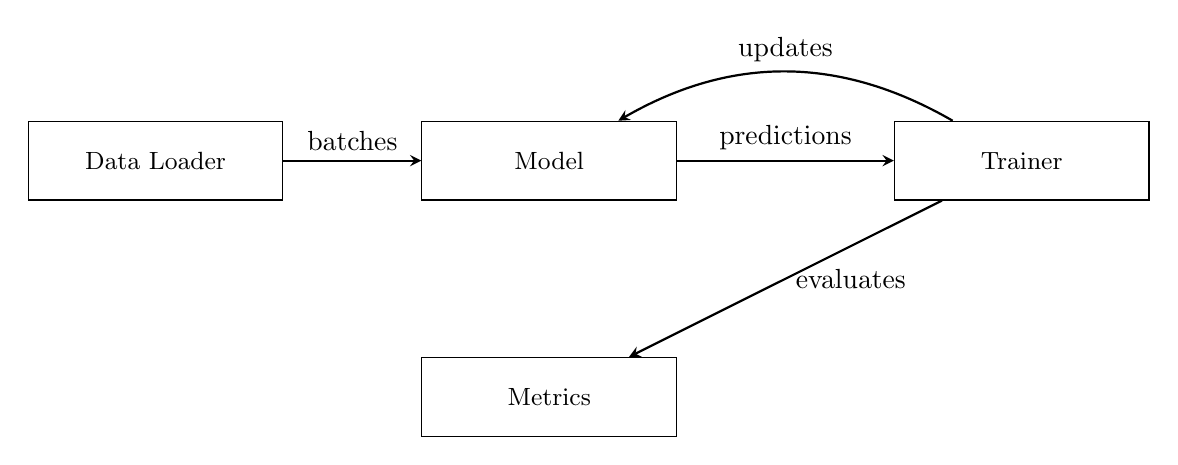
\begin{tikzpicture}[node distance=2cm, auto,
            block/.style={rectangle, draw, text width=3cm, text centered, minimum height=1cm, font=\small},
            arrow/.style={->, >=stealth, thick}]

        \node[block] (loader) {Data Loader};
        \node[block, right of=loader, node distance=5cm] (model) {Model};
        \node[block, right of=model, node distance=6cm] (trainer) {Trainer};
        \node[block, below of=model, node distance=3cm] (metrics) {Metrics};

        \draw[arrow] (loader) -- node[above] {batches} (model);
        \draw[arrow] (model) -- node[above] {predictions} (trainer);
        \draw[arrow] (trainer) -- node[right] {evaluates} (metrics);
        \draw[arrow] (trainer) to[bend right=30] node[above] {updates} (model);
    \end{tikzpicture}
    \caption{Component interaction during training.}
    \label{fig:component_interaction}
\end{figure}

The data loader provides batched hyperspectral images to the model.
The trainer orchestrates the training loop: it calls the model's forward pass, computes the loss, performs backpropagation, and updates model weights.
Metrics are computed periodically (typically each epoch) on the validation set to monitor training progress without affecting the optimization.

This separation ensures that each component has a single responsibility:
\begin{itemize}
    \item \textbf{Loader}: I/O and batching
    \item \textbf{Model}: Forward computation
    \item \textbf{Trainer}: Optimization loop and checkpointing
    \item \textbf{Metrics}: Evaluation
\end{itemize}

\subsection{Metrics}
All metrics are implemented in \mintinline{Python}|Code/metrics/metrics.py|.
\subsubsection{CompressionMetrics class}
The CompressionMetrics class provides static methods for evaluating hyperspectral image compression quality.
The metrics fall into two categories:
\begin{itemize}
    \item {\bf Spatial quality metrics}: MSE, RMSE, PSNR, SNR, and SSIM measure reconstruction fidelity in the spatial domain.
    \item {\bf Spectral quality metrics}: Spectral Angle Mapper (SAM) measures preservation of spectral signatures, which is critical for hyperspectral applications where spectral fidelity matters more than spatial appearance.
\end{itemize}
Additional methods compute compression-specific metrics: compression ratio (CR), bits per pixel (bpp), and bits per pixel per band (bpppb).
\subsubsection{Metrics and loss layer classes}
In addition to the static methods, the \mintinline{Python}|Code/metrics/metrics.py| file also contains several classes that implement the metrics as Keras layers.
These were created to speed up the computation of metrics during model training and evaluation.
The classes are: \mintinline{python}|MeanSquaredError|, \mintinline{python}|PeakSignalToNoiseRatio|, \mintinline{python}|StructualSimilarity| and \\ \mintinline{python}|SpectralAngle|.
Each of these classes inherits from the \mintinline{python}|tf.keras.layers.Layer| class and implements the respective metric in the \mintinline{python}|call| method.
\subsection{Data Loader}
The data loader is implemented in \mintinline{Python}|Code/TFDataloader/TFdataloader.py| as the TFHySpecNetLoader class.
This class utilizes TensorFlow's \mintinline{Python}|tf.data| pipeline to efficiently load and preprocess the HySpecNet-11k dataset.

The loader assumes hyperspectral data stored as NumPy files (\mintinline{bash}|.npy|) with band-major ordering, following the preprocessed format described in the external specification.
Dataset splits are defined by CSV files containing patch identifiers for training, validation, and test sets.

To avoid I/O bottlenecks during training, the loader uses parallel mapping \\(\mintinline{python}|tf.data.AUTOTUNE|) to load multiple files concurrently and prefetching to overlap data loading with model computation.
This design ensures that GPU utilization remains high even when loading large hyperspectral images from disk.

\subsection{Configuration and extensibility}
Model hyperparameters are stored in JSON configuration files (e.g.,\\ \mintinline{bash}|config/lineRWKV_config.json|) rather than being hardcoded.
This separation of configuration from code enables:
\begin{itemize}
    \item Running experiments with different hyperparameters without code changes
    \item Reproducing experiments by storing configuration alongside model weights
    \item Version control of experimental settings
\end{itemize}

To add a new compression model, the following components need to be implemented:
\begin{enumerate}
    \item A model class inheriting from \mintinline{Python}|tf.keras.Model| with \mintinline{Python}|encode| and \mintinline{Python}|decode| methods
    \item A trainer class following the pattern established by LineRWKVTrainer or RCGDNAETrainer
    \item A configuration file specifying model hyperparameters
\end{enumerate}

The existing metrics and data loader can be reused without modification, as they are model-agnostic.


% % TODO
\chapter{Machine learning model implementation}

\section{Machine learning basics}

\subsection{Neural networks}
Artificial neural networks (ANNs) are function approximators inspired by how people believed the human brain works.
They consist of layers of neurons that are interconnected via weighted connections.
Each neuron receives multiple inputs, applies a bias term and an activation function, which produces an output.
The simplified mathematical representation of a single neuron is given by equation \ref{fig:neuron_equation} :
\begin{align}
    y = \phi \left( \sum_{i=1}^{n} w_i x_i + b \right),
    \label{fig:neuron_equation}
\end{align}
where $y$ is the output of the neuron, $x_i$ are the inputs, $w_i$ are the weights associated with each input, $b$ is the bias term and $\phi$ is the activation function.
$\phi$ can be any non-linear differentiable function, as linear functions would simplify the model to only having one layer, while it needs to be differentiable due to the use of gradient-based optimization methods discussed in Section \ref{sec:training_nn}. \par
Typical activation functions include Rectified Linear Unit (ReLU), Sigmoid or Tanh.
In these, the models mostly used ReLU, Gaussian Error Linear Unit (GeLU), Leaky ReLU, and Sigmoid.
The ReLU, GeLU, and Leaky ReLU are similar functions that simply introduce non-linearity.
The most basic of these is the ReLU, which outputs zero for any negative input and the input itself for any positive input.
Leaky ReLU introduces a small slope for negative inputs instead of outputting zero.
GeLU is a smoother version of ReLU that approximates the output using the Gaussian error function, as shown in equation \ref{fig:gelu_equation}:
\begin{align}
    \text{GeLU}(x) = \frac{1}{2} x \left( 1 + \text{erf} \left( \frac{x}{\sqrt{2}} \right) \right),
    \label{fig:gelu_equation}
\end{align}
where $\text{erf}$ is the error function shown in equation \ref{fig:error_function_equation},
\begin{align}
    \text{erf}(x) = \frac{2}{\sqrt{\pi}} \int_{0}^{x} e^{-t^2} dt.
    \label{fig:error_function_equation}
\end{align}

The Sigmoid function, on the other hand, maps input values to a range between 0 and 1 which is useful for probabilistic outputs or other problems where a certain range of outputs is appropriate.
The Sigmoid function is given by the formula in equation \ref{fig:sigmoid_equation}:
\begin{align}
    \text{Sigmoid}(x) = \frac{1}{1 + e^{-x}}.
    \label{fig:sigmoid_equation}
\end{align}

\subsection{Training neural networks} \label{sec:training_nn}
Neural networks are typically trained using a process called backpropagation.
This involves calculating the gradient of a loss function with respect to the network's weights and biases using the chain rule of calculus.
These gradients can then be used to update the weights and biases of the neurons using optimization algorithms.
One of the most commonly used optimization algorithms is stochastic gradient descent (SGD), especially in the form of the Adam optimizer~\cite{Adam2014}, which was used in this thesis.
Adam combines the advantages of two other extensions of SGD: Adaptive Gradient Algorithm (AdaGrad) and Root Mean Square Propagation (RMSProp).
It computes adaptive learning rates for each parameter based on estimates of the first and second moments of the gradients.
However, to use Adam or any other gradient-based optimization method a suitable loss function must be used to quantify the difference between the predicted outputs of the network and the true target values.
Common loss functions for regression problems include Mean Squared Error (MSE) and Mean Absolute Error (MAE)~\cite{lossMetrics}.
In image compression tasks, MSE is often used as it directly measures the pixel-wise differences between the original and reconstructed images.
This doesn't always correlate well with human perception of image quality, so other metrics like those discussed in Section \ref{sec:eval_metrics} may also be considered during model evaluation.






% % TODO


% \begin{itemize}
%   \item concept of the system
%   \item system architecture
%   \item description of data structures (and data bases)
%   \item components, modules, libraries, resume of important classes (if used)
%   \item resume of important algorithms (if used)
%   \item details of implementation of selected parts
%   \item applied design patterns
%   \item UML diagrams
% \end{itemize}



% % % % % % % % % % % % % % % % % % % % % % % % % % % % % % % % % % % % 
% % To use the minted package, import the package:                    %
% % \usepackage{minted}                                               %
% % and compile with the shell escape                                 %
% % pdflatex -shell-escape main                                       %
% % % % % % % % % % % % % % % % % % % % % % % % % % % % % % % % % % % % 


% Use special environments for inline code, eg  \lstinline|int a;| (package \texttt{listings})% or  \mintinline{C++}|int a;| (package \texttt{minted})
% . Longer parts of code put in the figure environment, eg. code in Fig. \ref{fig:pseudocode:listings}% and Fig. \ref{fig:pseudocode:minted}
% . Very long listings–move to an appendix.


% \clearpage
% \begin{figure}
%   \centering
%   \begin{lstlisting}
% class test : public basic
% {
%     public:
%       test (int a);
%       friend std::ostream operator<<(std::ostream & s, 
%                                      const test & t);
%     protected:
%       int _a;  

% }; 
% \end{lstlisting}
%   \caption{Pseudocode in \texttt{listings}.}
%   \label{fig:pseudocode:listings}
% \end{figure}


\chapter{Lossless compression model: LineRWKV}

\section{Introduction}
The LineRWKV model is a neural network designed for lossless compression of HSIs.
It is based on the RWKV (Receptance Weighted Key Value) architecture, which combines the advantages of recurrent neural networks (RNNs) while incorporating the parallelizability of transformers.
The LineRWKV model is specifically adapted to process HSIs in a line-by-line manner, making it suitable for exploiting the spatial and spectral correlations present in hyperspectral data.
This model is considered lossless because it is designed to predict each pixel or line of the image based on the context provided by the preceding pixels or lines, while having an explicit recurrence that allows the decoder to exactly reproduce the predictions made by the encoder.
This allows the model to achieve near lossless performance, which, when combined with the entropy coding of the prediction residuals, results in effective lossless compression.
\section{Related works}
The RWKV architecture was introduced by Peng et al. ~\cite{RWKV} as a novel neural network architecture that combines the strengths of RNNs and transformers.
RWKV achieves linear complexity \( O(n) \) compared to the quadratic complexity \( O(n^2) \) of attention-based models, making it more efficient for long sequences.
The RWKV was then adapted for HSI lossless compression by Valsesia et al.~\cite{valsesia2024linerwkv} who created the original LineRWKV model.
The implementation presented in this thesis is based on their work but modified to better suit the specific dataset and requirements of this project.

\section{Model architecture}
The model takes as input a hyperspectral image of shape \([batch, 128, 128, 202]\) where 202 is the number of spectral bands, and 128x128 is the spatial dimension of the image patch.
The input is first projected to a working dimension (default \( dim=128 \)) using a dense layer.
This projected input is then processed through a stack of LineRWKVBlock layers (default: 4 blocks).
Finally, the output is projected back to the original number of channels using another dense layer to produce the predicted image.
The models architecture is present in Figure \ref{fig:linerwkv_architecture}.

\subsection{Overall structure}
The LineRWKV model processes the input image in a sequential manner, line by line along the height dimension.
For each line, the model processes the pixels from left to right, maintaining a state that captures the context from the previous pixels in the line.
The context not only includes information that the model has inferred but also the residuals, allowing the model to make accurate predictions.
Processing images line-by-line ensures that the model maintains causality, allowing the decoder to exactly reproduce the predictions made by the encoder.
This explicit recurrence is crucial for achieving lossless compression.
The main downside of this approach is its sequential processing along the height dimension, which limits parallelization across lines.
This may be seen as a limitation in synthetic scenarios, such as processing images on GPUs, where parallelization is key for performance.
However, in practical applications such as satellite data transmission, where images are often gathered line by line, it is a reasonable trade-off to make.

\subsection{RWKV block}
The core component of the LineRWKV model is the LineRWKVBlock, which implements the RWKV mechanism adapted for line-by-line processing.
The block consists of three main projections: Value, Receptance, and Channel Mix.
The Value projection determines what information to store in the state, while the Receptance projection acts as a gate controlling how much of the state influences the output.
The RWKV recurrence is implemented as follows:
\begin{align}
    s_t & = \text{decay} \cdot s_{t-1} + (1 - \text{decay}) \cdot v_t, \\
    y_t & = x_t + r_t \cdot s_t
\end{align}
where \( s_t \) is the accumulated state at position \( t \), \( v_t \) is the value at position \( t \), \( r_t \) is the receptance (gate) at position \( t \), and decay is a fixed parameter per block.
The recurrence is implemented using TensorFlow's \texttt{tf.scan} function to ensure explicit left-to-right processing along the width dimension of the image line.


\subsection{Predictor model}
The LineRWKVPredictor class encapsulates the overall model architecture.
It handles the line-by-line processing of the input image using a \texttt{tf.while\_loop} to iterate over the height dimension.
Within each iteration, the current line is processed through all RWKV blocks, maintaining the state across lines to capture temporal and spatial context.

\begin{figure}[h]
    \centering
    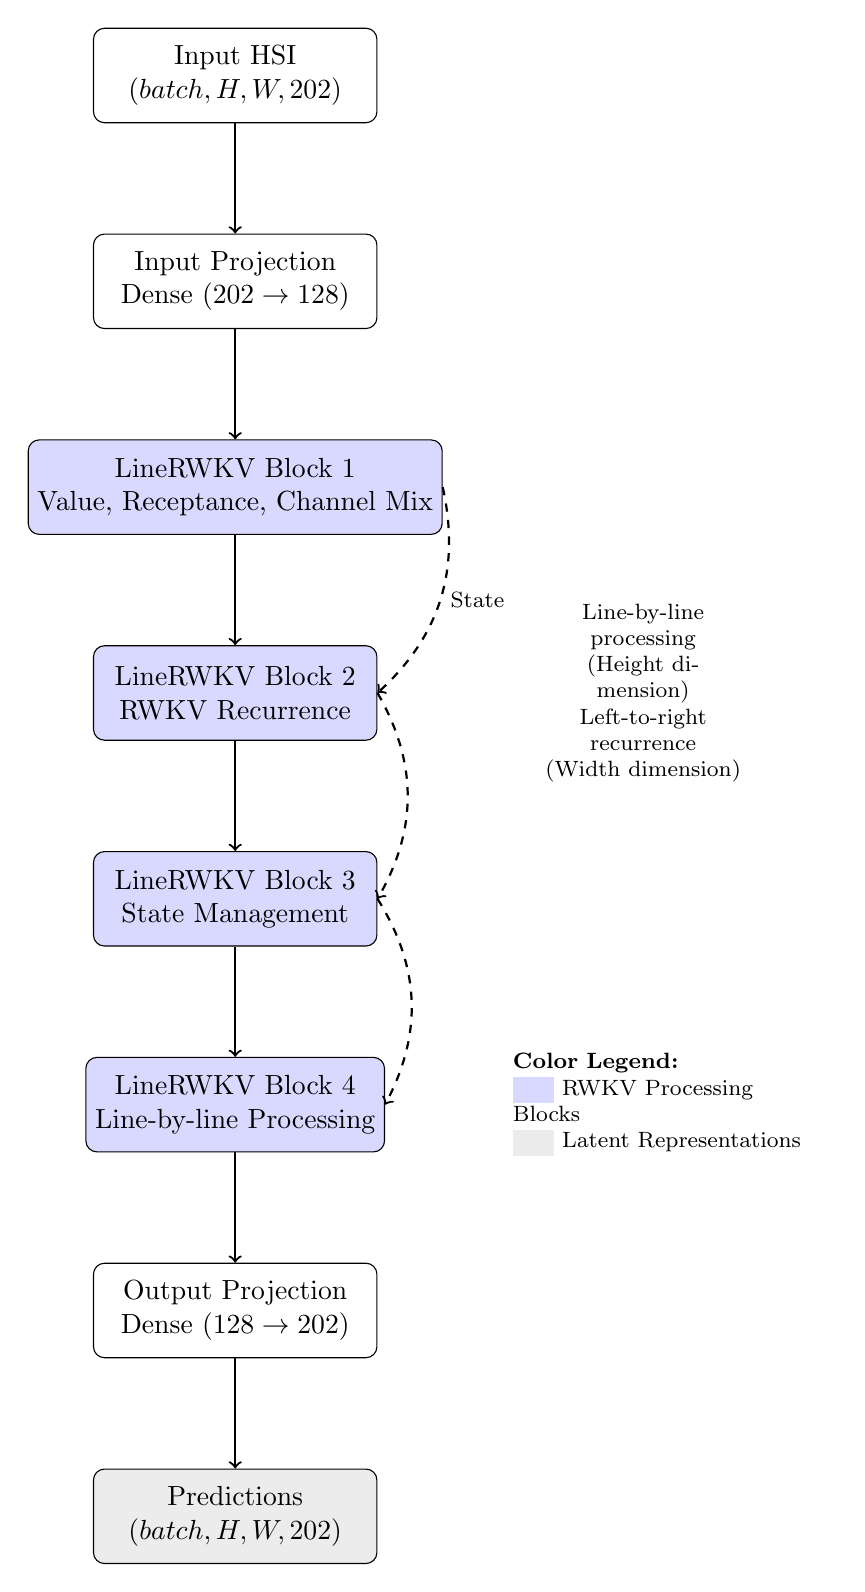
\begin{tikzpicture}[
            block/.style={draw, rounded corners, minimum width=3.6cm, minimum height=1.2cm, align=center},
            rwkvblock/.style={draw, rounded corners, minimum width=3.6cm, minimum height=1.2cm, align=center, fill=blue!15},
            latent/.style={draw, rounded corners, minimum width=3.6cm, minimum height=1.2cm, align=center, fill=gray!15},
            arrow/.style={->, thick},
            node distance=1.4cm
        ]

        \node[block] (input) {Input HSI\\$(batch, H, W, 202)$};

        \node[block, below=of input] (inputproj) {Input Projection\\Dense $(202 \to 128)$};

        \node[rwkvblock, below=of inputproj] (rwkv1) {LineRWKV Block 1\\Value, Receptance, Channel Mix};

        \node[rwkvblock, below=of rwkv1] (rwkv2) {LineRWKV Block 2\\RWKV Recurrence};

        \node[rwkvblock, below=of rwkv2] (rwkv3) {LineRWKV Block 3\\State Management};

        \node[rwkvblock, below=of rwkv3] (rwkv4) {LineRWKV Block 4\\Line-by-line Processing};

        \node[block, below=of rwkv4] (outputproj) {Output Projection\\Dense $(128 \to 202)$};

        \node[latent, below=of outputproj] (output) {Predictions\\$(batch, H, W, 202)$};

        % State flow arrows (curved)
        \draw[arrow, dashed, bend left=30] (rwkv1.east) to node[right, font=\footnotesize] {State} (rwkv2.east);
        \draw[arrow, dashed, bend left=30] (rwkv2.east) to (rwkv3.east);
        \draw[arrow, dashed, bend left=30] (rwkv3.east) to (rwkv4.east);

        % Main data flow
        \draw[arrow] (input) -- (inputproj);
        \draw[arrow] (inputproj) -- (rwkv1);
        \draw[arrow] (rwkv1) -- (rwkv2);
        \draw[arrow] (rwkv2) -- (rwkv3);
        \draw[arrow] (rwkv3) -- (rwkv4);
        \draw[arrow] (rwkv4) -- (outputproj);
        \draw[arrow] (outputproj) -- (output);

        % Side note for processing direction
        \node[right=2cm of rwkv2, text width=2.5cm, align=center, font=\footnotesize] (note) {Line-by-line\\processing\\(Height dimension)\\Left-to-right\\recurrence\\(Width dimension)};

        % Color legend
        \node[right=1.5cm of rwkv4, text width=4cm, align=left, font=\footnotesize] (legend) {
            \textbf{Color Legend:}\\
            \colorbox{blue!15}{\phantom{xx}} RWKV Processing Blocks\\
            \colorbox{gray!15}{\phantom{xx}} Latent Representations
        };

    \end{tikzpicture}
    \caption{LineRWKV architecture for lossless HSI compression. The model processes images line-by-line with explicit recurrence maintaining state across RWKV blocks.}
    \label{fig:linerwkv_architecture}
\end{figure}

\section{Model implementation}
One of the greatest differences between this implementation and the original LineRWKV implementation by Valsesia et al.~\cite{valsesia2024linerwkv} is the lack of using external programming languages such as CUDA for the RWKV block implementation.
Instead, this implementation relies solely on TensorFlow operations to ensure compatibility and ease of use.
This makes the implementation more accessible and easier to modify or extend.
The LineRWKV model is implemented in the file \texttt{lineRWKV.py} which contains the main classes: \texttt{LineRWKVBlock}, \texttt{LineRWKVPredictor}, and \texttt{LineRWKVLosslessCodec}.
The training logic is encapsulated in the \texttt{LineRWKVTrainer} class located in the file \\ \texttt{Code/lossless/lineRWKV\_trainer.py}.

\section{Training}
The LineRWKV model was trained using the Adam optimizer with a learning rate of 0.0001.
Mean Squared Error (MSE) was used as the loss function to quantify the difference between the original and predicted images.
The training process involved monitoring the loss on both the training and validation datasets to ensure proper convergence and to prevent overfitting.
The training curves for both training and validation metrics are shown in Figure \ref{fig:linerwkv_training_curves}.
\begin{figure}
    \centering

    \begin{subfigure}{0.45\textwidth}
        \centering
        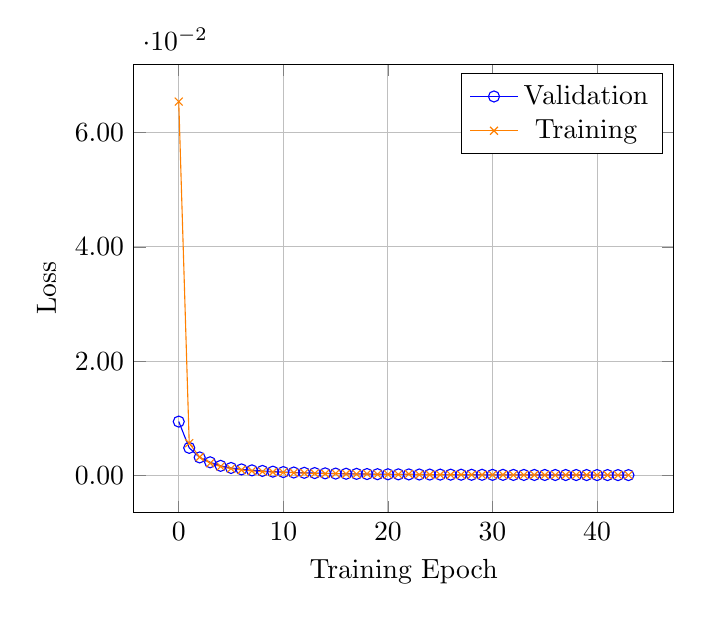
\begin{tikzpicture}
            \begin{axis}[
                    xlabel={Training Epoch},
                    ylabel={Loss},
                    grid=major,
                    y tick label style={
                            /pgf/number format/.cd,
                            fixed,
                            fixed zerofill,
                            precision=2,
                            /tikz/.cd
                        },
                    x tick label style={
                            /pgf/number format/.cd,
                            fixed,
                            fixed zerofill,
                            precision=0,
                            /tikz/.cd
                        }
                ]

                \addplot [color=blue, mark=o] coordinates {
                        (0, 0.009407560341060162)
                        (1, 0.004810214042663574)
                        (2, 0.0031330555211752653)
                        (3, 0.002282948000356555)
                        (4, 0.0016603863332420588)
                        (5, 0.0012889106292277575)
                        (6, 0.0010397301521152258)
                        (7, 0.0008686351939104497)
                        (8, 0.0007727619959041476)
                        (9, 0.00064383156131953)
                        (10, 0.0005692030536010861)
                        (11, 0.000493538158480078)
                        (12, 0.0004400104226078838)
                        (13, 0.0003951920662075281)
                        (14, 0.0003450929361861199)
                        (15, 0.00030338598298840225)
                        (16, 0.0002759403141681105)
                        (17, 0.00025547065888531506)
                        (18, 0.00022568783606402576)
                        (19, 0.00019690908084157854)
                        (20, 0.0001816522126318887)
                        (21, 0.0001718180428724736)
                        (22, 0.00015882171283010393)
                        (23, 0.0001460858475184068)
                        (24, 0.00013458446483127773)
                        (25, 0.00012411290663294494)
                        (26, 0.00011710380931617692)
                        (27, 0.00010621912952046841)
                        (28, 9.497698192717507e-05)
                        (29, 9.24327177926898e-05)
                        (30, 8.367952250409871e-05)
                        (31, 8.189443906303495e-05)
                        (32, 7.198640378192067e-05)
                        (33, 6.906240014359355e-05)
                        (34, 6.499591836472973e-05)
                        (35, 6.0125807067379355e-05)
                        (36, 5.752416473114863e-05)
                        (37, 5.3721520089311525e-05)
                        (38, 5.271703776088543e-05)
                        (39, 4.8286154196830466e-05)
                        (40, 4.4822023482993245e-05)
                        (41, 4.4321088353171945e-05)
                        (42, 3.9606144127901644e-05)
                        (43, 3.899712464772165e-05)
                    };
                \addlegendentry{Validation}

                \addplot [color=orange, mark=x] coordinates {
                        (0, 0.06543833017349243)
                        (1, 0.005621455144137144)
                        (2, 0.0032000713981688023)
                        (3, 0.0021202838979661465)
                        (4, 0.0015380382537841797)
                        (5, 0.001166594447568059)
                        (6, 0.000936653115786612)
                        (7, 0.0007651583873666823)
                        (8, 0.0006456300034187734)
                        (9, 0.0005646181525662541)
                        (10, 0.0005173908430151641)
                        (11, 0.0004485288809519261)
                        (12, 0.00040175634785555303)
                        (13, 0.0003316929214634001)
                        (14, 0.0002880409883800894)
                        (15, 0.00030707093537785113)
                        (16, 0.0002466256555635482)
                        (17, 0.0002117988478858024)
                        (18, 0.00023902875545900315)
                        (19, 0.00016381702153012156)
                        (20, 0.00016549444990232587)
                        (21, 0.00014241068856790662)
                        (22, 0.0002152604574803263)
                        (23, 0.00011299942707410082)
                        (24, 0.00010382891196059063)
                        (25, 9.793112985789776e-05)
                        (26, 9.01487801456824e-05)
                        (27, 0.00011477591033326462)
                        (28, 9.235702600562945e-05)
                        (29, 6.821603165008128e-05)
                        (30, 7.396235014311969e-05)
                        (31, 9.18613513931632e-05)
                        (32, 5.539982521440834e-05)
                        (33, 5.151082223164849e-05)
                        (34, 6.67546337353997e-05)
                        (35, 5.1719791372306645e-05)
                        (36, 4.2620449676178396e-05)
                        (37, 4.732586967293173e-05)
                        (38, 5.8244087995262817e-05)
                        (39, 3.697131251101382e-05)
                        (40, 3.350775295984931e-05)
                        (41, 4.449908374226652e-05)
                        (42, 3.0147257348289713e-05)
                        (43, 4.007069583167322e-05)
                    };
                \addlegendentry{Training}

            \end{axis}
        \end{tikzpicture}
        \caption{Loss over Epochs}
        \label{fig:linerwkv_loss}
    \end{subfigure}
    \hfill
    \begin{subfigure}{0.45\textwidth}
        \centering
        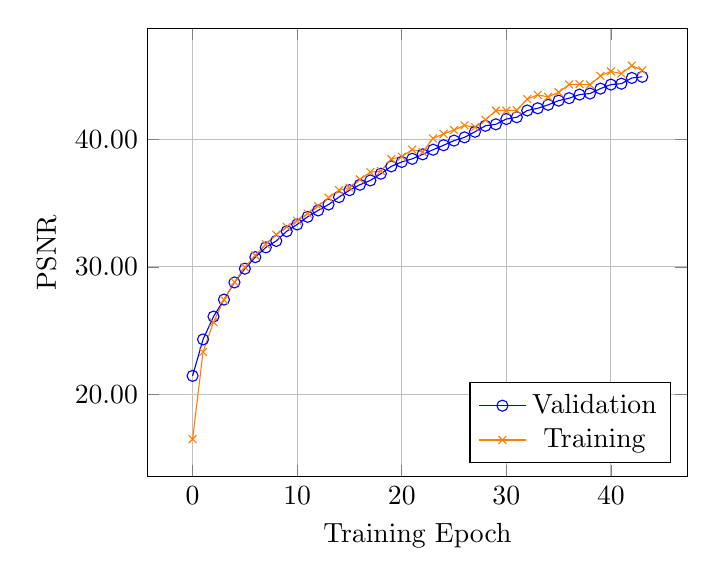
\begin{tikzpicture}
            \begin{axis}[
                    legend pos = south east,
                    xlabel={Training Epoch},
                    ylabel={PSNR},
                    grid=major,
                    y tick label style={
                            /pgf/number format/.cd,
                            fixed,
                            fixed zerofill,
                            precision=2,
                            /tikz/.cd
                        },
                    x tick label style={
                            /pgf/number format/.cd,
                            fixed,
                            fixed zerofill,
                            precision=0,
                            /tikz/.cd
                        }
                ]

                \addplot [color=blue, mark=o] coordinates {
                        (0, 21.4301815032959)
                        (1, 24.294260025024414)
                        (2, 26.08614158630371)
                        (3, 27.422435760498047)
                        (4, 28.771203994750977)
                        (5, 29.850343704223633)
                        (6, 30.758956909179688)
                        (7, 31.52450180053711)
                        (8, 32.031158447265625)
                        (9, 32.7913932800293)
                        (10, 33.3255615234375)
                        (11, 33.92399597167969)
                        (12, 34.42793273925781)
                        (13, 34.89232635498047)
                        (14, 35.47333526611328)
                        (15, 36.01667785644531)
                        (16, 36.444923400878906)
                        (17, 36.78514099121094)
                        (18, 37.311309814453125)
                        (19, 37.88816833496094)
                        (20, 38.23708724975586)
                        (21, 38.481483459472656)
                        (22, 38.8343391418457)
                        (23, 39.197044372558594)
                        (24, 39.5498046875)
                        (25, 39.914371490478516)
                        (26, 40.16914367675781)
                        (27, 40.604957580566406)
                        (28, 41.0752067565918)
                        (29, 41.192630767822266)
                        (30, 41.60801315307617)
                        (31, 41.74924850463867)
                        (32, 42.278480529785156)
                        (33, 42.452945709228516)
                        (34, 42.72536849975586)
                        (35, 43.05262756347656)
                        (36, 43.24553680419922)
                        (37, 43.528011322021484)
                        (38, 43.610416412353516)
                        (39, 43.99602127075195)
                        (40, 44.31494140625)
                        (41, 44.38319778442383)
                        (42, 44.83277130126953)
                        (43, 44.92425537109375)
                    };
                \addlegendentry{Validation}

                \addplot [color=orange, mark=x] coordinates {
                        (0, 16.45710563659668)
                        (1, 23.306358337402344)
                        (2, 25.658098220825195)
                        (3, 27.403240203857422)
                        (4, 28.795366287231445)
                        (5, 29.96370506286621)
                        (6, 30.90170669555664)
                        (7, 31.773481369018555)
                        (8, 32.526023864746094)
                        (9, 33.13193130493164)
                        (10, 33.613277435302734)
                        (11, 34.18340301513672)
                        (12, 34.767417907714844)
                        (13, 35.430030822753906)
                        (14, 36.01505661010742)
                        (15, 36.21891784667969)
                        (16, 36.8654899597168)
                        (17, 37.43046188354492)
                        (18, 37.51952362060547)
                        (19, 38.465450286865234)
                        (20, 38.65346908569336)
                        (21, 39.20689392089844)
                        (22, 39.0259895324707)
                        (23, 40.08292770385742)
                        (24, 40.44110107421875)
                        (25, 40.74326705932617)
                        (26, 41.11164855957031)
                        (27, 40.971431732177734)
                        (28, 41.54671859741211)
                        (29, 42.267616271972656)
                        (30, 42.26740264892578)
                        (31, 42.30288314819336)
                        (32, 43.175086975097656)
                        (33, 43.50278854370117)
                        (34, 43.34954071044922)
                        (35, 43.70232391357422)
                        (36, 44.3183708190918)
                        (37, 44.34353256225586)
                        (38, 44.300960540771484)
                        (39, 45.00051498413086)
                        (40, 45.346797943115234)
                        (41, 45.1777458190918)
                        (42, 45.806270599365234)
                        (43, 45.433204650878906)
                    };
                \addlegendentry{Training}

            \end{axis}
        \end{tikzpicture}
        \caption{PSNR over Epochs}
        \label{fig:linerwkv_psnr}
    \end{subfigure}

    \begin{subfigure}{0.45\textwidth}
        \centering
        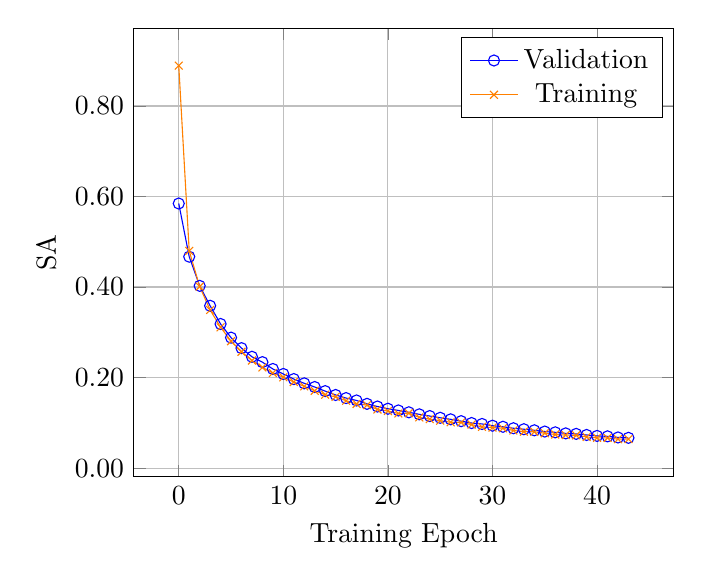
\begin{tikzpicture}
            \begin{axis}[
                    xlabel={Training Epoch},
                    ylabel={SA},
                    grid=major,
                    y tick label style={
                            /pgf/number format/.cd,
                            fixed,
                            fixed zerofill,
                            precision=2,
                            /tikz/.cd
                        },
                    x tick label style={
                            /pgf/number format/.cd,
                            fixed,
                            fixed zerofill,
                            precision=0,
                            /tikz/.cd
                        }
                ]

                \addplot [color=blue, mark=o] coordinates {
                        (0, 0.584546685218811)
                        (1, 0.4670645296573639)
                        (2, 0.40264245867729187)
                        (3, 0.358594685792923)
                        (4, 0.3184387981891632)
                        (5, 0.28829753398895264)
                        (6, 0.26505622267723083)
                        (7, 0.2459702491760254)
                        (8, 0.2341461330652237)
                        (9, 0.21901920437812805)
                        (10, 0.20802128314971924)
                        (11, 0.19677719473838806)
                        (12, 0.18732163310050964)
                        (13, 0.17921094596385956)
                        (14, 0.17015379667282104)
                        (15, 0.1616140604019165)
                        (16, 0.15476563572883606)
                        (17, 0.14950813353061676)
                        (18, 0.14199285209178925)
                        (19, 0.1361209750175476)
                        (20, 0.13124322891235352)
                        (21, 0.1274399310350418)
                        (22, 0.12335852533578873)
                        (23, 0.11884608119726181)
                        (24, 0.115072101354599)
                        (25, 0.11122660338878632)
                        (26, 0.10784369707107544)
                        (27, 0.10377958416938782)
                        (28, 0.09963683784008026)
                        (29, 0.09759838134050369)
                        (30, 0.09377550333738327)
                        (31, 0.09138836711645126)
                        (32, 0.08813308924436569)
                        (33, 0.0859752669930458)
                        (34, 0.08360479027032852)
                        (35, 0.08082777261734009)
                        (36, 0.07911476492881775)
                        (37, 0.076787568628788)
                        (38, 0.07567582279443741)
                        (39, 0.0732908770442009)
                        (40, 0.07121607661247253)
                        (41, 0.07024075090885162)
                        (42, 0.06776102632284164)
                        (43, 0.06693092733621597)
                    };
                \addlegendentry{Validation}

                \addplot [color=orange, mark=x] coordinates {
                        (0, 0.8891897797584534)
                        (1, 0.4799339771270752)
                        (2, 0.40103963017463684)
                        (3, 0.34944018721580505)
                        (4, 0.31118500232696533)
                        (5, 0.2803877890110016)
                        (6, 0.2570354640483856)
                        (7, 0.23769591748714447)
                        (8, 0.22247378528118134)
                        (9, 0.21014198660850525)
                        (10, 0.20072515308856964)
                        (11, 0.19033849239349365)
                        (12, 0.18060016632080078)
                        (13, 0.17091701924800873)
                        (14, 0.16223353147506714)
                        (15, 0.15750664472579956)
                        (16, 0.14889569580554962)
                        (17, 0.14176853001117706)
                        (18, 0.13934092223644257)
                        (19, 0.12958353757858276)
                        (20, 0.12617307901382446)
                        (21, 0.12065298855304718)
                        (22, 0.12148594856262207)
                        (23, 0.11204167455434799)
                        (24, 0.10828837007284164)
                        (25, 0.10487120598554611)
                        (26, 0.10130390524864197)
                        (27, 0.10100327432155609)
                        (28, 0.09617067128419876)
                        (29, 0.09117532521486282)
                        (30, 0.08960641175508499)
                        (31, 0.08810199797153473)
                        (32, 0.08316231518983841)
                        (33, 0.08067581802606583)
                        (34, 0.08027194440364838)
                        (35, 0.07713572680950165)
                        (36, 0.07431518286466599)
                        (37, 0.07304374873638153)
                        (38, 0.07244901359081268)
                        (39, 0.06883850693702698)
                        (40, 0.06694726645946503)
                        (41, 0.06673319637775421)
                        (42, 0.06397014111280441)
                        (43, 0.06412291526794434)
                    };
                \addlegendentry{Training}

            \end{axis}
        \end{tikzpicture}
        \caption{SA over Epochs}
        \label{fig:linerwkv_sa}
    \end{subfigure}
    \hfill
    \begin{subfigure}{0.45\textwidth}
        \centering
        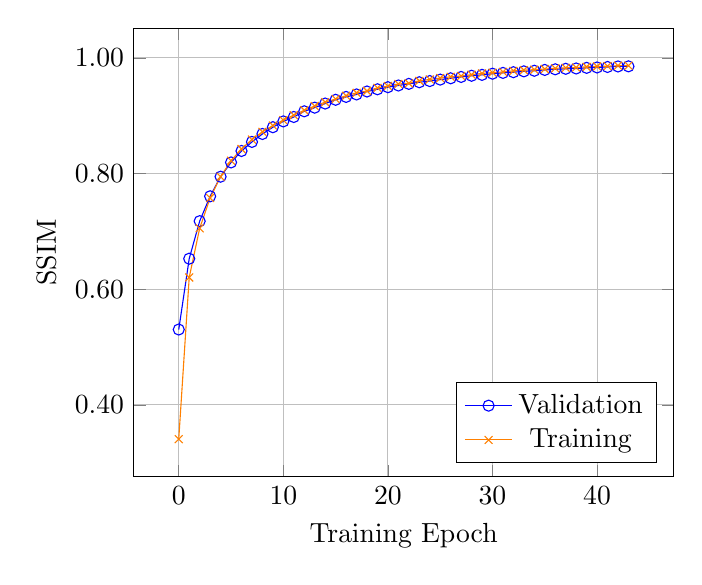
\begin{tikzpicture}
            \begin{axis}[
                    legend pos = south east,
                    xlabel={Training Epoch},
                    ylabel={SSIM},
                    grid=major,
                    y tick label style={
                            /pgf/number format/.cd,
                            fixed,
                            fixed zerofill,
                            precision=2,
                            /tikz/.cd
                        },
                    x tick label style={
                            /pgf/number format/.cd,
                            fixed,
                            fixed zerofill,
                            precision=0,
                            /tikz/.cd
                        }
                ]

                \addplot [color=blue, mark=o] coordinates {
                        (0, 0.5302415490150452)
                        (1, 0.6527398228645325)
                        (2, 0.7176406979560852)
                        (3, 0.7606276273727417)
                        (4, 0.7945206165313721)
                        (5, 0.8191938996315002)
                        (6, 0.8389992117881775)
                        (7, 0.8546600341796875)
                        (8, 0.8684037327766418)
                        (9, 0.8800985813140869)
                        (10, 0.8901407122612)
                        (11, 0.8977642059326172)
                        (12, 0.9075806140899658)
                        (13, 0.9139000773429871)
                        (14, 0.9210157990455627)
                        (15, 0.9275243282318115)
                        (16, 0.9324974417686462)
                        (17, 0.9367613792419434)
                        (18, 0.9418460726737976)
                        (19, 0.9456820487976074)
                        (20, 0.9493062496185303)
                        (21, 0.9522435665130615)
                        (22, 0.9550524353981018)
                        (23, 0.9578432440757751)
                        (24, 0.9598869681358337)
                        (25, 0.962399423122406)
                        (26, 0.9646883010864258)
                        (27, 0.9670284390449524)
                        (28, 0.9690667986869812)
                        (29, 0.9706171154975891)
                        (30, 0.9726284742355347)
                        (31, 0.9740246534347534)
                        (32, 0.9752240180969238)
                        (33, 0.9766833186149597)
                        (34, 0.9777167439460754)
                        (35, 0.9791537523269653)
                        (36, 0.9802177548408508)
                        (37, 0.9811046719551086)
                        (38, 0.9816390872001648)
                        (39, 0.9827482104301453)
                        (40, 0.9834092259407043)
                        (41, 0.9842660427093506)
                        (42, 0.985164225101471)
                        (43, 0.9853312373161316)
                    };
                \addlegendentry{Validation}

                \addplot [color=orange, mark=x] coordinates {
                        (0, 0.3406010866165161)
                        (1, 0.6202467679977417)
                        (2, 0.7053083181381226)
                        (3, 0.7576161623001099)
                        (4, 0.794639527797699)
                        (5, 0.8221554756164551)
                        (6, 0.8423802256584167)
                        (7, 0.8587701320648193)
                        (8, 0.8720710873603821)
                        (9, 0.8829948306083679)
                        (10, 0.8922829627990723)
                        (11, 0.9010712504386902)
                        (12, 0.9093681573867798)
                        (13, 0.9167277216911316)
                        (14, 0.9234001040458679)
                        (15, 0.9288172721862793)
                        (16, 0.9345059990882874)
                        (17, 0.9396138191223145)
                        (18, 0.9427030086517334)
                        (19, 0.948157012462616)
                        (20, 0.9513996243476868)
                        (21, 0.9548333287239075)
                        (22, 0.9559947848320007)
                        (23, 0.9603119492530823)
                        (24, 0.9627232551574707)
                        (25, 0.9650713205337524)
                        (26, 0.9673001766204834)
                        (27, 0.9686068892478943)
                        (28, 0.9709581732749939)
                        (29, 0.9731282591819763)
                        (30, 0.974493145942688)
                        (31, 0.9757099747657776)
                        (32, 0.9775499701499939)
                        (33, 0.9787697196006775)
                        (34, 0.9795756936073303)
                        (35, 0.980737566947937)
                        (36, 0.9819249510765076)
                        (37, 0.9827708005905151)
                        (38, 0.983360767364502)
                        (39, 0.9844467639923096)
                        (40, 0.9852024912834167)
                        (41, 0.9856505393981934)
                        (42, 0.9864423274993896)
                        (43, 0.9866632223129272)
                    };
                \addlegendentry{Training}

            \end{axis}
        \end{tikzpicture}
        \caption{SSIM over Epochs}
        \label{fig:linerwkv_ssim}
    \end{subfigure}

    \caption{Training and Validation Metrics over Epochs for LineRWKV model}
    \label{fig:linerwkv_training_curves}
\end{figure}

The training was conducted over 44 epochs, with the model showing consistent improvement in all monitored metrics.
Such a specific number of epochs was chosen due to time constraints rather than convergence criteria.
The training was stopped early because of limited computational resources and time constraints.
Due to such early termination of training, none of the metrics started to plateau, indicating that the model could benefit from further training to achieve even better performance.

\section{Summary}
The LineRWKV model presents a paper-faithful implementation of the RWKV architecture tailored for hyperspectral image lossless compression.
The model effectively captures the spatial and spectral correlations present in HSI data while maintaining the causality necessary for lossless compression.
It processes images line-by-line, allowing it to exploit the inherent structure of hyperspectral images.

\chapter{Lossy compression model: Residual Convolutional Autoencoders}\label{sec:RCAE}
\section{Introduction}
An autoencoder is a type of neural network used for unsupervised learning, with the primary application in data compression and representation~\cite{li2018autoencoderbasedresidualdeep, barman2022autoencoders}.
Its structure mainly consists of two main parts: an encoder and a decoder.
The encoder compresses the high-dimensional input data into a lower latent representation called the bottleneck.
The decoder, on the other hand, reconstructs compressed data back to its original form.
The network is trained to minimize the difference between the input data and its reconstructed output, typically using a loss function such as MSE.
For the purpose of this thesis, two custom autoencoder architectures were implemented that were loosely inspired by existing solutions

\section{Related works}
For image data, the standard autoencoder architecture is inefficient due to the high dimensionality and spatial structure of images.
Convolutional Autoencoders (CAEs) overcome these limitations by replacing fully connected layers with convolutional layers in both the encoder and decoder.
In an encoder, convolutional layers progressively reduce the spatial dimensions of the image while increasing the depth.
The decoder performs the reverse operation using transposed convolutional layers or upsampling layers to reconstruct the image to its original size.
This architecture is very effective in capturing spatial patterns and features in images, including HSI~\cite{barman2022autoencoders}.
\section{Model architecture}
The Residual Convolutional Autoencoder (RCAE) enhances the standard CAE architecture by incorporating residual blocks, popularized by ResNet models~\cite{ResNet}.
The residual blocks incorporate skip connections that allow for bypassing one or more layers.
These blocks learn the residual mapping, which is the difference between the input and the output, rather than a full transformation.
This helps to mitigate the vanishing gradient problem and allows for training deeper networks more effectively.
The designed architectures are presented in Figure \ref{fig:res3d_autoencoder} for 3D CNN, and in Figure \ref{fig:rcae2D1D_architecture} for the hybrid 2D-1D CNN.

\section{Residual blocks}
The core functionality of residual blocks is the shortcut connection.
In a traditional network without residual connections, it is designed to learn a direct mapping from input \( x \) to output \( H(x) \).
The residual block, instead of learning \( H(x) \) directly, learns the residual function \( F(x) = H(x) - x \).
The original input \( x \) is then added to the output of these layers, making the final output \( H(x) = F(x) + x \).
This approach creates a clear pathway for information and gradients to flow through the network.

\section{Residual Convolutional Autoencoder architecture}
Two main different RCAE models were implemented in this thesis: a RCAE3D with a residual block and a hybrid 2D-1D RCAE also with residual blocks.

\subsection{RCAE3D}
The architecture that was implemented in this thesis is an unsymmetrical RCAE.
It follows the general structure of an autoencoder with an encoder and a decoder, with the addition of residual blocks between convolutional layers.
The network uses 3D convolutional layers to capture both spatial and spectral features of HSI data.
While the overall structure is similar to traditional CAEs, some modifications were made that allow it to distinguish itself from standard implementations.
The first of them is the use of 3D convolutional kernels with a depth of 1, which makes the model process each spectral band separately, treating spectral dimensions as separate channels.
This approach reduces computational complexity.
The second modification is the use of sigmoid activation in the latent space to constrain the bottleneck values between 0 and 1.
The last modification is the use of double upsampling in the decoder part to better reconstruct the image as well as to reduce checkerboard artifacts.

\begin{figure}[h]
    \centering

    % ================= ENCODER =================
    \begin{minipage}{0.48\linewidth}
        \centering
        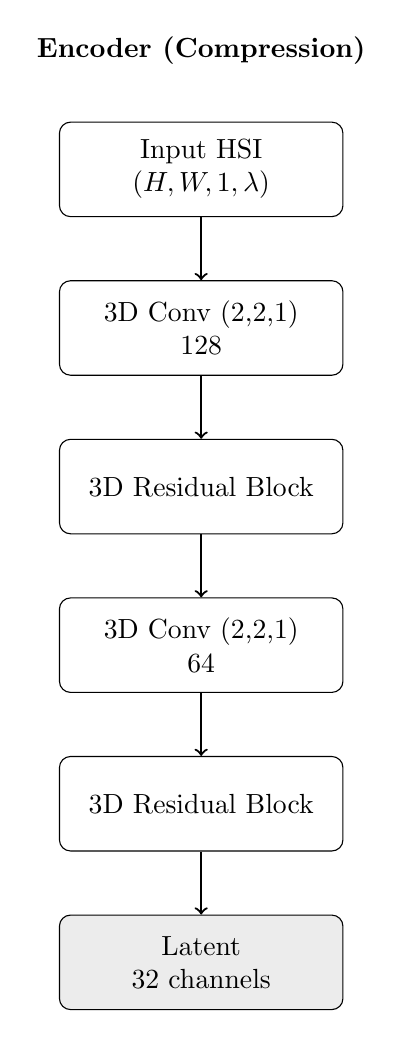
\begin{tikzpicture}[
                block/.style={draw, rounded corners, minimum width=3.6cm, minimum height=1.2cm, align=center},
                latent/.style={draw, rounded corners, minimum width=3.6cm, minimum height=1.2cm, align=center, fill=gray!15},
                arrow/.style={->, thick},
                node distance=0.8cm
            ]

            \node[block] (input) {Input HSI\\$(H,W,1,\lambda)$};

            \node[block, below=of input] (conv1) {3D Conv (2,2,1)\\128};

            \node[block, below=of conv1] (res1) {3D Residual Block};

            \node[block, below=of res1] (conv2) {3D Conv (2,2,1)\\64};

            \node[block, below=of conv2] (res2) {3D Residual Block};

            \node[latent, below=of res2] (latent) {Latent\\32 channels};

            \draw[arrow] (input) -- (conv1);
            \draw[arrow] (conv1) -- (res1);
            \draw[arrow] (res1) -- (conv2);
            \draw[arrow] (conv2) -- (res2);
            \draw[arrow] (res2) -- (latent);

            \node[above=0.6cm of input] {\textbf{Encoder (Compression)}};

        \end{tikzpicture}
    \end{minipage}
    \hfill
    % ================= DECODER =================
    \begin{minipage}{0.48\linewidth}
        \centering
        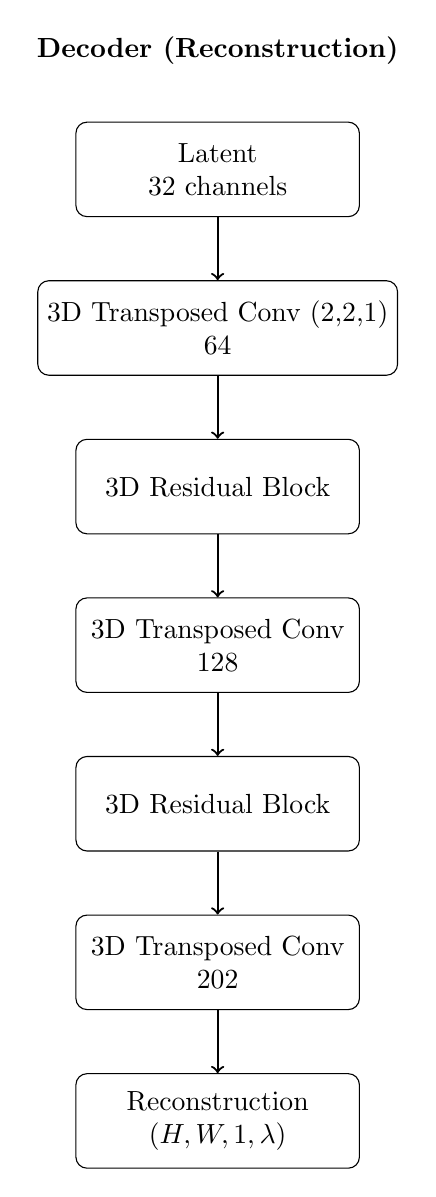
\begin{tikzpicture}[
                block/.style={draw, rounded corners, minimum width=3.6cm, minimum height=1.2cm, align=center},
                arrow/.style={->, thick},
                node distance=0.8cm
            ]

            \node[block] (latent2) {Latent\\32 channels};

            \node[block, below=of latent2] (tconv1) {3D Transposed Conv (2,2,1)\\64};

            \node[block, below=of tconv1] (res3) {3D Residual Block};

            \node[block, below=of res3] (tconv2) {3D Transposed Conv\\128};

            \node[block, below=of tconv2] (res4) {3D Residual Block};

            \node[block, below=of res4] (tconv3) {3D Transposed Conv\\202};

            \node[block, below=of tconv3] (output) {Reconstruction\\$(H,W,1,\lambda)$};

            \draw[arrow] (latent2) -- (tconv1);
            \draw[arrow] (tconv1) -- (res3);
            \draw[arrow] (res3) -- (tconv2);
            \draw[arrow] (tconv2) -- (res4);
            \draw[arrow] (res4) -- (tconv3);
            \draw[arrow] (tconv3) -- (output);

            \node[above=0.6cm of latent2] {\textbf{Decoder (Reconstruction)}};

        \end{tikzpicture}
    \end{minipage}

    \caption{RCAE3D architecture. Left: encoder. Right: decoder. $\lambda$ is the number of spectral bands.}
    \label{fig:res3d_autoencoder}
\end{figure}

\begin{figure}[h]
    \centering
    \begin{subfigure}{0.45\textwidth}
        \centering
        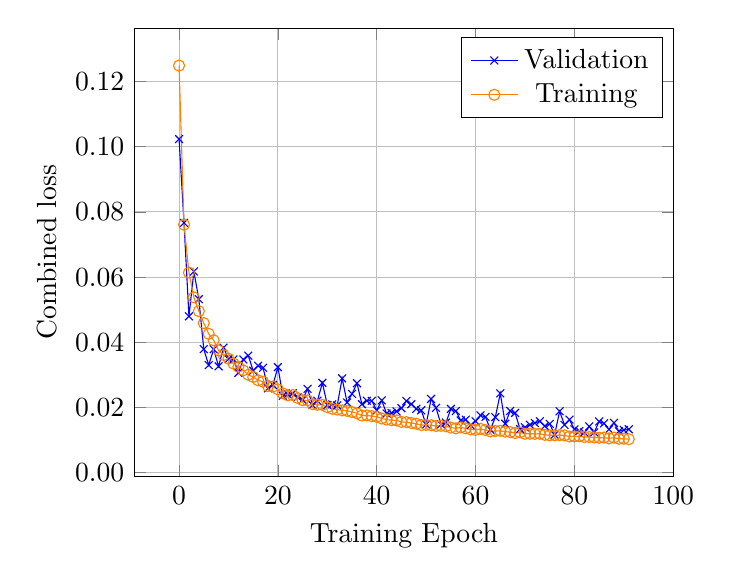
\begin{tikzpicture}
            \begin{axis}[
                    xlabel={Training Epoch},
                    ylabel={Combined loss},
                    grid=major,
                    y tick label style={
                            /pgf/number format/.cd,
                            fixed,
                            fixed zerofill,
                            precision=2,
                            /tikz/.cd
                        },
                    x tick label style={
                            /pgf/number format/.cd,
                            fixed,
                            fixed zerofill,
                            precision=0,
                            /tikz/.cd
                        }
                ]

                \addplot [color=blue, mark=x] coordinates {
                        (0, 0.10235235840082169)
                        (1, 0.07663942128419876)
                        (2, 0.04798494651913643)
                        (3, 0.06174611300230026)
                        (4, 0.05324003845453262)
                        (5, 0.03791242465376854)
                        (6, 0.033029817044734955)
                        (7, 0.037872422486543655)
                        (8, 0.03263986110687256)
                        (9, 0.03838342800736427)
                        (10, 0.03486507385969162)
                        (11, 0.034777794033288956)
                        (12, 0.030641645193099976)
                        (13, 0.03473419323563576)
                        (14, 0.03591570258140564)
                        (15, 0.03131246566772461)
                        (16, 0.03281250223517418)
                        (17, 0.03221651911735535)
                        (18, 0.025881636887788773)
                        (19, 0.026979567483067513)
                        (20, 0.03240417316555977)
                        (21, 0.023591626435518265)
                        (22, 0.024047726765275)
                        (23, 0.024385148659348488)
                        (24, 0.023186465725302696)
                        (25, 0.02236579731106758)
                        (26, 0.025740643963217735)
                        (27, 0.020771745592355728)
                        (28, 0.022094853222370148)
                        (29, 0.027572255581617355)
                        (30, 0.02079709619283676)
                        (31, 0.020970316603779793)
                        (32, 0.020654931664466858)
                        (33, 0.028946856036782265)
                        (34, 0.021554086357355118)
                        (35, 0.024206336587667465)
                        (36, 0.02746562659740448)
                        (37, 0.021038232371211052)
                        (38, 0.02210572175681591)
                        (39, 0.02205815352499485)
                        (40, 0.019139405339956284)
                        (41, 0.022203762084245682)
                        (42, 0.018161941319704056)
                        (43, 0.018360765650868416)
                        (44, 0.01880485564470291)
                        (45, 0.019807027652859688)
                        (46, 0.022022653371095657)
                        (47, 0.02103755809366703)
                        (48, 0.019623128697276115)
                        (49, 0.01916258968412876)
                        (50, 0.014798787422478199)
                        (51, 0.022660091519355774)
                        (52, 0.01991870440542698)
                        (53, 0.01485351100564003)
                        (54, 0.015403526835143566)
                        (55, 0.019592072814702988)
                        (56, 0.01894526742398739)
                        (57, 0.016038211062550545)
                        (58, 0.01629628799855709)
                        (59, 0.014584698714315891)
                        (60, 0.015795210376381874)
                        (61, 0.017591221258044243)
                        (62, 0.017152920365333557)
                        (63, 0.013225697912275791)
                        (64, 0.01706155575811863)
                        (65, 0.024361910298466682)
                        (66, 0.015040675178170204)
                        (67, 0.01897529698908329)
                        (68, 0.018359627574682236)
                        (69, 0.013400017283856869)
                        (70, 0.013950377702713013)
                        (71, 0.014718557707965374)
                        (72, 0.015267486684024334)
                        (73, 0.015800148248672485)
                        (74, 0.01433536782860756)
                        (75, 0.014998660422861576)
                        (76, 0.011677310802042484)
                        (77, 0.018864767625927925)
                        (78, 0.014697214588522911)
                        (79, 0.01629389077425003)
                        (80, 0.013314533978700638)
                        (81, 0.012795081362128258)
                        (82, 0.012369396165013313)
                        (83, 0.014239709824323654)
                        (84, 0.012393578886985779)
                        (85, 0.015749577432870865)
                        (86, 0.015146649442613125)
                        (87, 0.013304057531058788)
                        (88, 0.015294109471142292)
                        (89, 0.0127038499340415)
                        (90, 0.013130868785083294)
                        (91, 0.013342203572392464)
                    };
                \addlegendentry{Validation}
                \addplot [color=orange, mark=o] coordinates {
                        (0, 0.12488876283168793)
                        (1, 0.0760994702577591)
                        (2, 0.06139294058084488)
                        (3, 0.05379967391490936)
                        (4, 0.049570370465517044)
                        (5, 0.04590107128024101)
                        (6, 0.042613886296749115)
                        (7, 0.0406462736427784)
                        (8, 0.037496455013751984)
                        (9, 0.036114685237407684)
                        (10, 0.03499366343021393)
                        (11, 0.033496830612421036)
                        (12, 0.03250383213162422)
                        (13, 0.03142219036817551)
                        (14, 0.0300611462444067)
                        (15, 0.029382362961769104)
                        (16, 0.02835644967854023)
                        (17, 0.02792113460600376)
                        (18, 0.026568058878183365)
                        (19, 0.02642497420310974)
                        (20, 0.02557828277349472)
                        (21, 0.02436554990708828)
                        (22, 0.0237562395632267)
                        (23, 0.023838292807340622)
                        (24, 0.022945009171962738)
                        (25, 0.022257372736930847)
                        (26, 0.022202586755156517)
                        (27, 0.021060731261968613)
                        (28, 0.02086048386991024)
                        (29, 0.020808611065149307)
                        (30, 0.02013709768652916)
                        (31, 0.01963484287261963)
                        (32, 0.019373230636119843)
                        (33, 0.019138580188155174)
                        (34, 0.01898401975631714)
                        (35, 0.018637990579009056)
                        (36, 0.018237300217151642)
                        (37, 0.017536209896206856)
                        (38, 0.01760024018585682)
                        (39, 0.017369918525218964)
                        (40, 0.01718665100634098)
                        (41, 0.01665506139397621)
                        (42, 0.016308030113577843)
                        (43, 0.016108786687254906)
                        (44, 0.016079140827059746)
                        (45, 0.01559080183506012)
                        (46, 0.015527111478149891)
                        (47, 0.015260367654263973)
                        (48, 0.015042640268802643)
                        (49, 0.014620519243180752)
                        (50, 0.014684377238154411)
                        (51, 0.014585019089281559)
                        (52, 0.014333085156977177)
                        (53, 0.014410736970603466)
                        (54, 0.014282961376011372)
                        (55, 0.01385787595063448)
                        (56, 0.013617221266031265)
                        (57, 0.013911168090999126)
                        (58, 0.013622848317027092)
                        (59, 0.01330544799566269)
                        (60, 0.013157435692846775)
                        (61, 0.013470842503011227)
                        (62, 0.013101020827889442)
                        (63, 0.01267982181161642)
                        (64, 0.012808465398848057)
                        (65, 0.012874647043645382)
                        (66, 0.012617851607501507)
                        (67, 0.012468879111111164)
                        (68, 0.012186259962618351)
                        (69, 0.012384030967950821)
                        (70, 0.011957209557294846)
                        (71, 0.011979496106505394)
                        (72, 0.01193330716341734)
                        (73, 0.011968623846769333)
                        (74, 0.011631444096565247)
                        (75, 0.011483830399811268)
                        (76, 0.011495801620185375)
                        (77, 0.011541340500116348)
                        (78, 0.011471623554825783)
                        (79, 0.011115348897874355)
                        (80, 0.011160047724843025)
                        (81, 0.01121483650058508)
                        (82, 0.010964750312268734)
                        (83, 0.010964056476950645)
                        (84, 0.010843283496797085)
                        (85, 0.0107354037463665)
                        (86, 0.010789698921144009)
                        (87, 0.010550170205533504)
                        (88, 0.010778834111988544)
                        (89, 0.010427636094391346)
                        (90, 0.0104448227211833)
                        (91, 0.010301770642399788)
                    };
                \addlegendentry{Training}
            \end{axis}
        \end{tikzpicture}
        \caption{Combined loss over Epochs}
        \label{fig:lossrcae3D}
    \end{subfigure}
    \hfill
    \begin{subfigure}{0.45\textwidth}
        \centering
        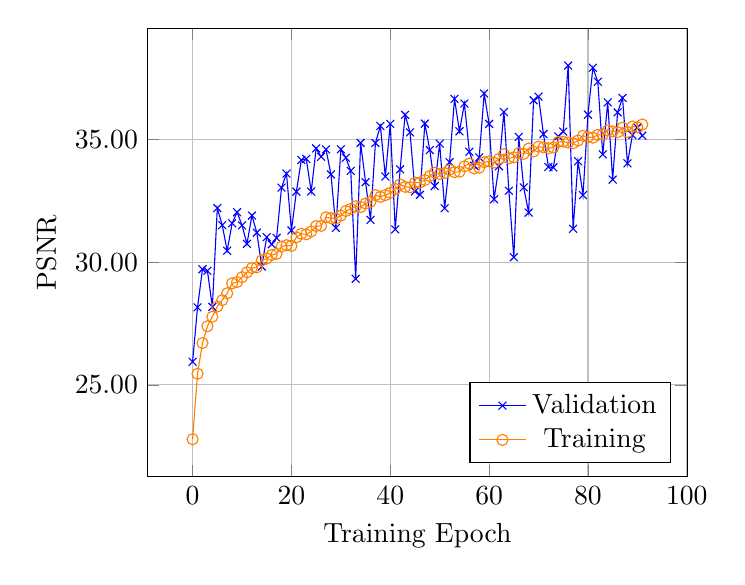
\begin{tikzpicture}
            \begin{axis}[
                    legend pos = south east,
                    xlabel={Training Epoch},
                    ylabel={PSNR},
                    grid=major,
                    y tick label style={
                            /pgf/number format/.cd,
                            fixed,
                            fixed zerofill,
                            precision=2,
                            /tikz/.cd
                        },
                    x tick label style={
                            /pgf/number format/.cd,
                            fixed,
                            fixed zerofill,
                            precision=0,
                            /tikz/.cd
                        }
                ]

                \addplot [color=blue, mark=x] coordinates {
                        (0, 25.93950653076172)
                        (1, 28.160022735595703)
                        (2, 29.71485137939453)
                        (3, 29.655838012695312)
                        (4, 28.18056297302246)
                        (5, 32.21288299560547)
                        (6, 31.51291275024414)
                        (7, 30.471261978149414)
                        (8, 31.59086799621582)
                        (9, 32.044551849365234)
                        (10, 31.50766372680664)
                        (11, 30.753538131713867)
                        (12, 31.905317306518555)
                        (13, 31.20844268798828)
                        (14, 29.825851440429688)
                        (15, 31.029144287109375)
                        (16, 30.733741760253906)
                        (17, 30.994752883911133)
                        (18, 33.04856872558594)
                        (19, 33.6215705871582)
                        (20, 31.299461364746094)
                        (21, 32.88441848754883)
                        (22, 34.17299270629883)
                        (23, 34.21745300292969)
                        (24, 32.88846206665039)
                        (25, 34.64767837524414)
                        (26, 34.3051643371582)
                        (27, 34.605587005615234)
                        (28, 33.584617614746094)
                        (29, 31.40159797668457)
                        (30, 34.61219024658203)
                        (31, 34.2663688659668)
                        (32, 33.730201721191406)
                        (33, 29.325767517089844)
                        (34, 34.87262725830078)
                        (35, 33.26871109008789)
                        (36, 31.730712890625)
                        (37, 34.869754791259766)
                        (38, 35.561153411865234)
                        (39, 33.50170135498047)
                        (40, 35.65048599243164)
                        (41, 31.34166145324707)
                        (42, 33.79373550415039)
                        (43, 36.0163459777832)
                        (44, 35.30113983154297)
                        (45, 32.892372131347656)
                        (46, 32.75322723388672)
                        (47, 35.65812301635742)
                        (48, 34.579864501953125)
                        (49, 33.111839294433594)
                        (50, 34.841251373291016)
                        (51, 32.20612335205078)
                        (52, 34.08606719970703)
                        (53, 36.66917419433594)
                        (54, 35.34701919555664)
                        (55, 36.47772216796875)
                        (56, 34.51277542114258)
                        (57, 33.93871307373047)
                        (58, 34.27887725830078)
                        (59, 36.88798141479492)
                        (60, 35.64904022216797)
                        (61, 32.57314682006836)
                        (62, 33.920284271240234)
                        (63, 36.13347625732422)
                        (64, 32.91972351074219)
                        (65, 30.208030700683594)
                        (66, 35.11776351928711)
                        (67, 33.055511474609375)
                        (68, 32.028438568115234)
                        (69, 36.610347747802734)
                        (70, 36.76143264770508)
                        (71, 35.23411560058594)
                        (72, 33.8880500793457)
                        (73, 33.87153244018555)
                        (74, 35.13802719116211)
                        (75, 35.33442687988281)
                        (76, 38.027400970458984)
                        (77, 31.36670684814453)
                        (78, 34.12306594848633)
                        (79, 32.74388885498047)
                        (80, 36.02290344238281)
                        (81, 37.936927795410156)
                        (82, 37.365848541259766)
                        (83, 34.401607513427734)
                        (84, 36.52416229248047)
                        (85, 33.374855041503906)
                        (86, 36.119407653808594)
                        (87, 36.70569610595703)
                        (88, 34.03816604614258)
                        (89, 35.193267822265625)
                        (90, 35.50403594970703)
                        (91, 35.16654968261719)
                    };
                \addlegendentry{Validation}
                \addplot [color=orange, mark=o] coordinates {
                        (0, 22.780628204345703)
                        (1, 25.451433181762695)
                        (2, 26.702850341796875)
                        (3, 27.390409469604492)
                        (4, 27.779829025268555)
                        (5, 28.191431045532227)
                        (6, 28.454715728759766)
                        (7, 28.735572814941406)
                        (8, 29.13907814025879)
                        (9, 29.19483184814453)
                        (10, 29.392637252807617)
                        (11, 29.589996337890625)
                        (12, 29.76430320739746)
                        (13, 29.79458999633789)
                        (14, 30.079269409179688)
                        (15, 30.151960372924805)
                        (16, 30.296871185302734)
                        (17, 30.346330642700195)
                        (18, 30.63947868347168)
                        (19, 30.695056915283203)
                        (20, 30.66988182067871)
                        (21, 31.018274307250977)
                        (22, 31.16248321533203)
                        (23, 31.14145851135254)
                        (24, 31.257728576660156)
                        (25, 31.479307174682617)
                        (26, 31.486743927001953)
                        (27, 31.833982467651367)
                        (28, 31.801916122436523)
                        (29, 31.786745071411133)
                        (30, 31.905921936035156)
                        (31, 32.09162902832031)
                        (32, 32.17900466918945)
                        (33, 32.28458786010742)
                        (34, 32.25422286987305)
                        (35, 32.39927291870117)
                        (36, 32.47034454345703)
                        (37, 32.73967361450195)
                        (38, 32.66964340209961)
                        (39, 32.738609313964844)
                        (40, 32.835025787353516)
                        (41, 32.99176025390625)
                        (42, 33.17801284790039)
                        (43, 33.077850341796875)
                        (44, 33.058509826660156)
                        (45, 33.24728012084961)
                        (46, 33.25527572631836)
                        (47, 33.35476303100586)
                        (48, 33.52029800415039)
                        (49, 33.65394973754883)
                        (50, 33.60142517089844)
                        (51, 33.64293670654297)
                        (52, 33.77840042114258)
                        (53, 33.67938232421875)
                        (54, 33.695133209228516)
                        (55, 33.91791534423828)
                        (56, 34.02542495727539)
                        (57, 33.83184051513672)
                        (58, 33.860389709472656)
                        (59, 34.0860710144043)
                        (60, 34.118492126464844)
                        (61, 34.06855010986328)
                        (62, 34.21888732910156)
                        (63, 34.41295623779297)
                        (64, 34.24269104003906)
                        (65, 34.285640716552734)
                        (66, 34.45481872558594)
                        (67, 34.428401947021484)
                        (68, 34.641326904296875)
                        (69, 34.5222282409668)
                        (70, 34.71968078613281)
                        (71, 34.69059753417969)
                        (72, 34.65119934082031)
                        (73, 34.68873596191406)
                        (74, 34.91203308105469)
                        (75, 34.925437927246094)
                        (76, 34.88568115234375)
                        (77, 34.85721206665039)
                        (78, 34.96971130371094)
                        (79, 35.16022491455078)
                        (80, 35.113216400146484)
                        (81, 35.085472106933594)
                        (82, 35.1977653503418)
                        (83, 35.215885162353516)
                        (84, 35.38072204589844)
                        (85, 35.34075927734375)
                        (86, 35.31082534790039)
                        (87, 35.49381637573242)
                        (88, 35.319583892822266)
                        (89, 35.54022979736328)
                        (90, 35.50889205932617)
                        (91, 35.62568664550781)
                    };
                \addlegendentry{Training}
            \end{axis}
        \end{tikzpicture}
        \caption{PSNR over Epochs}
        \label{fig:psnrcae3D}
    \end{subfigure}


    \begin{subfigure}{0.45\textwidth}
        \centering
        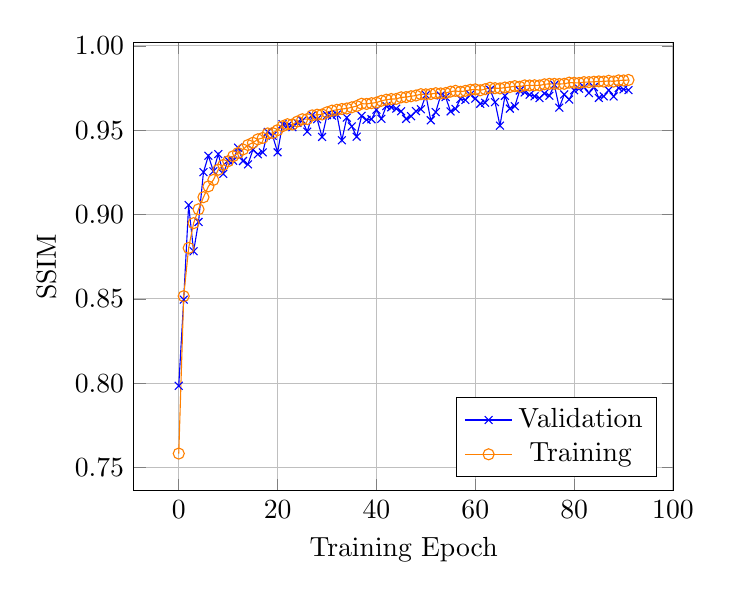
\begin{tikzpicture}
            \begin{axis}[
                    legend pos = south east,
                    xlabel={Training Epoch},
                    ylabel={SSIM},
                    grid=major,
                    y tick label style={
                            /pgf/number format/.cd,
                            fixed,
                            fixed zerofill,
                            precision=2,
                            /tikz/.cd
                        },
                    x tick label style={
                            /pgf/number format/.cd,
                            fixed,
                            fixed zerofill,
                            precision=0,
                            /tikz/.cd
                        }
                ]

                \addplot [color=blue, mark=x] coordinates {
                        (0, 0.7984480261802673)
                        (1, 0.8495583534240723)
                        (2, 0.9056621789932251)
                        (3, 0.878190279006958)
                        (4, 0.8955631256103516)
                        (5, 0.9250925183296204)
                        (6, 0.9348369836807251)
                        (7, 0.9256396293640137)
                        (8, 0.935814380645752)
                        (9, 0.9240951538085938)
                        (10, 0.9320598840713501)
                        (11, 0.9319164752960205)
                        (12, 0.9396477341651917)
                        (13, 0.9317298531532288)
                        (14, 0.929722785949707)
                        (15, 0.9383792877197266)
                        (16, 0.9357296824455261)
                        (17, 0.9368409514427185)
                        (18, 0.948954701423645)
                        (19, 0.9466593265533447)
                        (20, 0.9368625283241272)
                        (21, 0.953514575958252)
                        (22, 0.9526327848434448)
                        (23, 0.9517807364463806)
                        (24, 0.9543337821960449)
                        (25, 0.9556887745857239)
                        (26, 0.9490917921066284)
                        (27, 0.9588841795921326)
                        (28, 0.9564904570579529)
                        (29, 0.9459952712059021)
                        (30, 0.9588940739631653)
                        (31, 0.9586013555526733)
                        (32, 0.959254801273346)
                        (33, 0.9440140724182129)
                        (34, 0.9574071168899536)
                        (35, 0.9522408246994019)
                        (36, 0.9461192488670349)
                        (37, 0.9584800601005554)
                        (38, 0.9561277627944946)
                        (39, 0.9564850330352783)
                        (40, 0.9620845317840576)
                        (41, 0.956707239151001)
                        (42, 0.9642722010612488)
                        (43, 0.9635849595069885)
                        (44, 0.9627671837806702)
                        (45, 0.9612100124359131)
                        (46, 0.9566764235496521)
                        (47, 0.9582542777061462)
                        (48, 0.9612956047058105)
                        (49, 0.9624198079109192)
                        (50, 0.9708207249641418)
                        (51, 0.9558610320091248)
                        (52, 0.9607250690460205)
                        (53, 0.970539927482605)
                        (54, 0.9696164131164551)
                        (55, 0.9610934853553772)
                        (56, 0.9625731110572815)
                        (57, 0.968529999256134)
                        (58, 0.9678977131843567)
                        (59, 0.9710673093795776)
                        (60, 0.968756914138794)
                        (61, 0.9656156301498413)
                        (62, 0.9662632942199707)
                        (63, 0.9738762974739075)
                        (64, 0.9666366577148438)
                        (65, 0.9526463747024536)
                        (66, 0.970336377620697)
                        (67, 0.9627652764320374)
                        (68, 0.9642063975334167)
                        (69, 0.9734882116317749)
                        (70, 0.9723984003067017)
                        (71, 0.9709540605545044)
                        (72, 0.9700709581375122)
                        (73, 0.9690166711807251)
                        (74, 0.9717646241188049)
                        (75, 0.9704062342643738)
                        (76, 0.9768412113189697)
                        (77, 0.9633245468139648)
                        (78, 0.9711469411849976)
                        (79, 0.9681599736213684)
                        (80, 0.9736770391464233)
                        (81, 0.974608838558197)
                        (82, 0.9754930138587952)
                        (83, 0.972015380859375)
                        (84, 0.9755244851112366)
                        (85, 0.9691082239151001)
                        (86, 0.9700235724449158)
                        (87, 0.9736639857292175)
                        (88, 0.9699784517288208)
                        (89, 0.975011944770813)
                        (90, 0.9741803407669067)
                        (91, 0.9737376570701599)
                    };
                \addlegendentry{Validation}
                \addplot [color=orange, mark=o] coordinates {
                        (0, 0.7582841515541077)
                        (1, 0.8515803217887878)
                        (2, 0.8801500201225281)
                        (3, 0.8948519825935364)
                        (4, 0.9030926823616028)
                        (5, 0.9102505445480347)
                        (6, 0.9166759252548218)
                        (7, 0.9205020666122437)
                        (8, 0.9265837669372559)
                        (9, 0.9293701648712158)
                        (10, 0.9315764307975769)
                        (11, 0.934525728225708)
                        (12, 0.9364669322967529)
                        (13, 0.9385649561882019)
                        (14, 0.9411871433258057)
                        (15, 0.9425392150878906)
                        (16, 0.9445621967315674)
                        (17, 0.945412278175354)
                        (18, 0.9480618238449097)
                        (19, 0.9482972621917725)
                        (20, 0.9499978423118591)
                        (21, 0.95234614610672)
                        (22, 0.9535186886787415)
                        (23, 0.9533934593200684)
                        (24, 0.9551148414611816)
                        (25, 0.9564584493637085)
                        (26, 0.95656418800354)
                        (27, 0.9587551951408386)
                        (28, 0.9591631889343262)
                        (29, 0.9593079686164856)
                        (30, 0.960597038269043)
                        (31, 0.9615871906280518)
                        (32, 0.9620687961578369)
                        (33, 0.9625409245491028)
                        (34, 0.9628422856330872)
                        (35, 0.9635252356529236)
                        (36, 0.9643051028251648)
                        (37, 0.965656042098999)
                        (38, 0.9655482769012451)
                        (39, 0.9659722447395325)
                        (40, 0.9663354158401489)
                        (41, 0.9673973917961121)
                        (42, 0.9680601954460144)
                        (43, 0.9684544205665588)
                        (44, 0.9685096144676208)
                        (45, 0.9694580435752869)
                        (46, 0.9695835709571838)
                        (47, 0.970091700553894)
                        (48, 0.9705305099487305)
                        (49, 0.9713402390480042)
                        (50, 0.9712300896644592)
                        (51, 0.9714229106903076)
                        (52, 0.9719040393829346)
                        (53, 0.971765398979187)
                        (54, 0.9720104336738586)
                        (55, 0.9728376269340515)
                        (56, 0.9732948541641235)
                        (57, 0.972746729850769)
                        (58, 0.9733060002326965)
                        (59, 0.9739184975624084)
                        (60, 0.9741976261138916)
                        (61, 0.9736058712005615)
                        (62, 0.9743040204048157)
                        (63, 0.9751301407814026)
                        (64, 0.9748831391334534)
                        (65, 0.9747586846351624)
                        (66, 0.9752616882324219)
                        (67, 0.9755380153656006)
                        (68, 0.9760944247245789)
                        (69, 0.9757164120674133)
                        (70, 0.9765305519104004)
                        (71, 0.9764891266822815)
                        (72, 0.9765926599502563)
                        (73, 0.9765051007270813)
                        (74, 0.9771724939346313)
                        (75, 0.9774525165557861)
                        (76, 0.9774370193481445)
                        (77, 0.9773469567298889)
                        (78, 0.9774752855300903)
                        (79, 0.9781729578971863)
                        (80, 0.9780892729759216)
                        (81, 0.9779806137084961)
                        (82, 0.9784759283065796)
                        (83, 0.9784640669822693)
                        (84, 0.9787029027938843)
                        (85, 0.9789102673530579)
                        (86, 0.9788070917129517)
                        (87, 0.9792630672454834)
                        (88, 0.9788240790367126)
                        (89, 0.979510486125946)
                        (90, 0.979471743106842)
                        (91, 0.9797563552856445)
                    };
                \addlegendentry{Training}
            \end{axis}
        \end{tikzpicture}
        \caption{SSIM over Epochs}
        \label{fig:ssimrcae3D}
    \end{subfigure}
    \hfill
    \begin{subfigure}{0.45\textwidth}
        \centering
        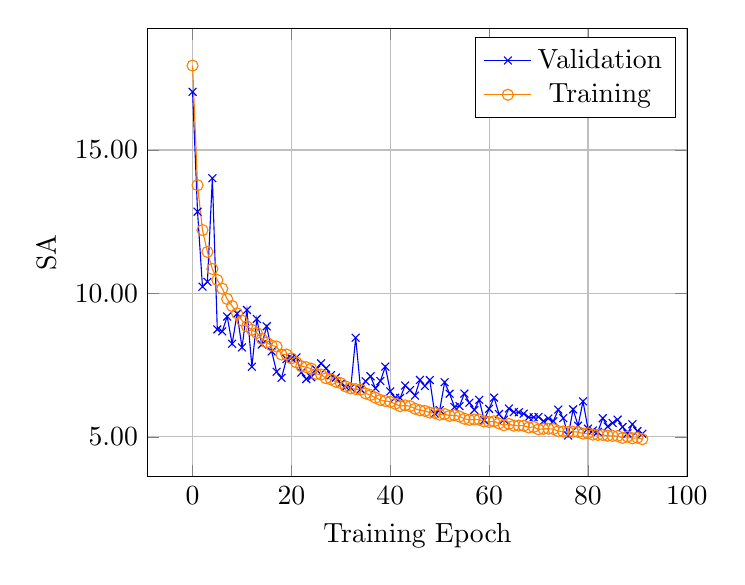
\begin{tikzpicture}
            \begin{axis}[
                    xlabel={Training Epoch},
                    ylabel={SA},
                    grid=major,
                    y tick label style={
                            /pgf/number format/.cd,
                            fixed,
                            fixed zerofill,
                            precision=2,
                            /tikz/.cd
                        },
                    x tick label style={
                            /pgf/number format/.cd,
                            fixed,
                            fixed zerofill,
                            precision=0,
                            /tikz/.cd
                        }
                ]

                \addplot [color=blue, mark=x] coordinates {
                        (0, 17.029129028320312)
                        (1, 12.850081443786621)
                        (2, 10.2352294921875)
                        (3, 10.402682304382324)
                        (4, 14.018712997436523)
                        (5, 8.74415111541748)
                        (6, 8.675470352172852)
                        (7, 9.193655014038086)
                        (8, 8.242999076843262)
                        (9, 9.292834281921387)
                        (10, 8.116047859191895)
                        (11, 9.422816276550293)
                        (12, 7.4433064460754395)
                        (13, 9.111153602600098)
                        (14, 8.22031021118164)
                        (15, 8.854507446289062)
                        (16, 7.97713565826416)
                        (17, 7.268143177032471)
                        (18, 7.055769443511963)
                        (19, 7.711036205291748)
                        (20, 7.74094295501709)
                        (21, 7.767396926879883)
                        (22, 7.241484642028809)
                        (23, 7.015998363494873)
                        (24, 7.077960014343262)
                        (25, 7.342684268951416)
                        (26, 7.562474250793457)
                        (27, 7.388894557952881)
                        (28, 7.149660110473633)
                        (29, 7.064121246337891)
                        (30, 6.853702545166016)
                        (31, 6.737691402435303)
                        (32, 6.704551696777344)
                        (33, 8.454350471496582)
                        (34, 6.653517723083496)
                        (35, 6.936152458190918)
                        (36, 7.110200881958008)
                        (37, 6.688652992248535)
                        (38, 6.944708824157715)
                        (39, 7.4467926025390625)
                        (40, 6.584795951843262)
                        (41, 6.362302303314209)
                        (42, 6.351436614990234)
                        (43, 6.787749767303467)
                        (44, 6.625823974609375)
                        (45, 6.436537265777588)
                        (46, 6.983758926391602)
                        (47, 6.7718963623046875)
                        (48, 6.977773189544678)
                        (49, 5.80666971206665)
                        (50, 5.931126117706299)
                        (51, 6.901595592498779)
                        (52, 6.503664493560791)
                        (53, 6.0370330810546875)
                        (54, 6.069291114807129)
                        (55, 6.506755352020264)
                        (56, 6.188706398010254)
                        (57, 5.936033248901367)
                        (58, 6.288683891296387)
                        (59, 5.579225063323975)
                        (60, 5.975053310394287)
                        (61, 6.367936611175537)
                        (62, 5.79392671585083)
                        (63, 5.599621295928955)
                        (64, 5.985958576202393)
                        (65, 5.863409996032715)
                        (66, 5.8533244132995605)
                        (67, 5.8037824630737305)
                        (68, 5.682488441467285)
                        (69, 5.681718826293945)
                        (70, 5.694751262664795)
                        (71, 5.5434250831604)
                        (72, 5.636937141418457)
                        (73, 5.541834831237793)
                        (74, 5.947728157043457)
                        (75, 5.652588367462158)
                        (76, 5.044161796569824)
                        (77, 5.956216335296631)
                        (78, 5.386303424835205)
                        (79, 6.2370219230651855)
                        (80, 5.283429145812988)
                        (81, 5.219955921173096)
                        (82, 5.171684265136719)
                        (83, 5.647566318511963)
                        (84, 5.358541011810303)
                        (85, 5.4812912940979)
                        (86, 5.598155498504639)
                        (87, 5.343461036682129)
                        (88, 5.116254806518555)
                        (89, 5.438146591186523)
                        (90, 5.197676181793213)
                        (91, 5.106213569641113)
                    };
                \addlegendentry{Validation}
                \addplot [color=orange, mark=o] coordinates {
                        (0, 17.94504165649414)
                        (1, 13.775412559509277)
                        (2, 12.208585739135742)
                        (3, 11.446345329284668)
                        (4, 10.852606773376465)
                        (5, 10.465799331665039)
                        (6, 10.167786598205566)
                        (7, 9.80573558807373)
                        (8, 9.561735153198242)
                        (9, 9.30470085144043)
                        (10, 9.052810668945312)
                        (11, 8.851577758789062)
                        (12, 8.729787826538086)
                        (13, 8.620124816894531)
                        (14, 8.413862228393555)
                        (15, 8.29115104675293)
                        (16, 8.184135437011719)
                        (17, 8.149025917053223)
                        (18, 7.86812686920166)
                        (19, 7.8697028160095215)
                        (20, 7.737522602081299)
                        (21, 7.595877647399902)
                        (22, 7.464798927307129)
                        (23, 7.426061630249023)
                        (24, 7.377140522003174)
                        (25, 7.194005489349365)
                        (26, 7.170656681060791)
                        (27, 7.04364013671875)
                        (28, 7.0006914138793945)
                        (29, 6.91839599609375)
                        (30, 6.868251800537109)
                        (31, 6.752579212188721)
                        (32, 6.687321186065674)
                        (33, 6.661233425140381)
                        (34, 6.6436238288879395)
                        (35, 6.513688087463379)
                        (36, 6.455100059509277)
                        (37, 6.362466812133789)
                        (38, 6.284783363342285)
                        (39, 6.250688076019287)
                        (40, 6.2180657386779785)
                        (41, 6.150066375732422)
                        (42, 6.066990375518799)
                        (43, 6.095996856689453)
                        (44, 6.06876802444458)
                        (45, 5.979491233825684)
                        (46, 5.925561428070068)
                        (47, 5.901834964752197)
                        (48, 5.843629360198975)
                        (49, 5.829334259033203)
                        (50, 5.771942138671875)
                        (51, 5.79197883605957)
                        (52, 5.731321811676025)
                        (53, 5.757233142852783)
                        (54, 5.707279682159424)
                        (55, 5.631196022033691)
                        (56, 5.59070348739624)
                        (57, 5.60506534576416)
                        (58, 5.594956874847412)
                        (59, 5.532016754150391)
                        (60, 5.516204357147217)
                        (61, 5.54024076461792)
                        (62, 5.4656147956848145)
                        (63, 5.402472019195557)
                        (64, 5.449939250946045)
                        (65, 5.387170791625977)
                        (66, 5.390438556671143)
                        (67, 5.3867669105529785)
                        (68, 5.324282646179199)
                        (69, 5.341182708740234)
                        (70, 5.2589569091796875)
                        (71, 5.27789306640625)
                        (72, 5.282555103302002)
                        (73, 5.269347190856934)
                        (74, 5.198698043823242)
                        (75, 5.1851115226745605)
                        (76, 5.164889812469482)
                        (77, 5.176820755004883)
                        (78, 5.166152000427246)
                        (79, 5.1105852127075195)
                        (80, 5.120883464813232)
                        (81, 5.075171947479248)
                        (82, 5.066224098205566)
                        (83, 5.064756393432617)
                        (84, 5.036619663238525)
                        (85, 5.030372619628906)
                        (86, 5.025725364685059)
                        (87, 4.96017599105835)
                        (88, 5.007492542266846)
                        (89, 4.947083473205566)
                        (90, 4.9669389724731445)
                        (91, 4.916675090789795)
                    };
                \addlegendentry{Training}
            \end{axis}
        \end{tikzpicture}
        \caption{Spectral Angle over Epochs}
        \label{fig:sarcae3D}
    \end{subfigure}

    \begin{subfigure}{0.45\textwidth}
        \centering
        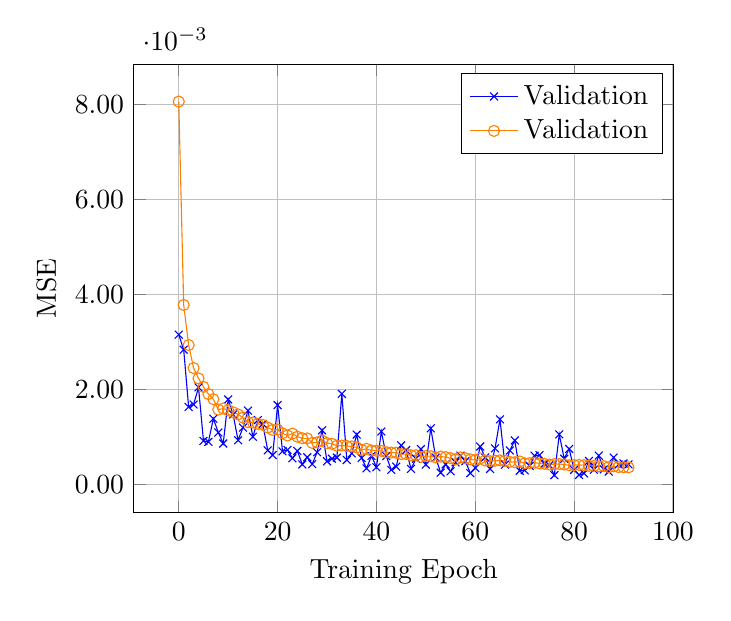
\begin{tikzpicture}
            \begin{axis}[
                    xlabel={Training Epoch},
                    ylabel={MSE},
                    grid=major,
                    y tick label style={
                            /pgf/number format/.cd,
                            fixed,
                            fixed zerofill,
                            precision=2,
                            /tikz/.cd
                        },
                    x tick label style={
                            /pgf/number format/.cd,
                            fixed,
                            fixed zerofill,
                            precision=0,
                            /tikz/.cd
                        }
                ]

                \addplot [color=blue, mark=x] coordinates {
                        (0, 0.0031531224958598614)
                        (1, 0.0028372795786708593)
                        (2, 0.0016320600407198071)
                        (3, 0.001683403505012393)
                        (4, 0.0020434632897377014)
                        (5, 0.0009169271215796471)
                        (6, 0.0008969841874204576)
                        (7, 0.0013845735229551792)
                        (8, 0.0010939451167359948)
                        (9, 0.0008622338064014912)
                        (10, 0.001789917703717947)
                        (11, 0.00147205067332834)
                        (12, 0.0009311611065641046)
                        (13, 0.0011981639545410872)
                        (14, 0.0015545592177659273)
                        (15, 0.00100420240778476)
                        (16, 0.00135508191306144)
                        (17, 0.0012737747747451067)
                        (18, 0.0007177647785283625)
                        (19, 0.00061859714332968)
                        (20, 0.0016711422940716147)
                        (21, 0.0006974503048695624)
                        (22, 0.000728204904589802)
                        (23, 0.0005511576309800148)
                        (24, 0.0007063893135637045)
                        (25, 0.00042094901436939836)
                        (26, 0.0005729408585466444)
                        (27, 0.0004275095707271248)
                        (28, 0.0006796438246965408)
                        (29, 0.001140041509643197)
                        (30, 0.0004877022292930633)
                        (31, 0.0005422760150395334)
                        (32, 0.0005648296209983528)
                        (33, 0.001907935133203864)
                        (34, 0.0005154599784873426)
                        (35, 0.0006538659799844027)
                        (36, 0.0010505170794203877)
                        (37, 0.0005568585474975407)
                        (38, 0.0003388614277355373)
                        (39, 0.0006012336234562099)
                        (40, 0.00036282508517615497)
                        (41, 0.0011143580777570605)
                        (42, 0.0005963052390143275)
                        (43, 0.00030664008227176964)
                        (44, 0.0003762863634619862)
                        (45, 0.0008237830479629338)
                        (46, 0.0007221039268188179)
                        (47, 0.00032896961783990264)
                        (48, 0.0005423359107226133)
                        (49, 0.0007446548552252352)
                        (50, 0.0004184590943623334)
                        (51, 0.00118138431571424)
                        (52, 0.000562822911888361)
                        (53, 0.0002472918713465333)
                        (54, 0.0004233366344124079)
                        (55, 0.00027767999563366175)
                        (56, 0.0004637854581233114)
                        (57, 0.0006069245282560587)
                        (58, 0.0004899875493720174)
                        (59, 0.00023725602659396827)
                        (60, 0.000347170076565817)
                        (61, 0.0007982627139426768)
                        (62, 0.0005687755765393376)
                        (63, 0.0003276124771218747)
                        (64, 0.0007596905343234539)
                        (65, 0.0013701709685847163)
                        (66, 0.0004173899651505053)
                        (67, 0.0007159101660363376)
                        (68, 0.0009259458165615797)
                        (69, 0.0002879009989555925)
                        (70, 0.00029868847923353314)
                        (71, 0.00039140915032476187)
                        (72, 0.0006061852909624577)
                        (73, 0.0006175654125399888)
                        (74, 0.0004351300885900855)
                        (75, 0.0004039695777464658)
                        (76, 0.00019599913503043354)
                        (77, 0.001054333639331162)
                        (78, 0.0005411037127487361)
                        (79, 0.00074784952448681)
                        (80, 0.00030608693487010896)
                        (81, 0.00019974031602032483)
                        (82, 0.00023198216513264924)
                        (83, 0.0004948008572682738)
                        (84, 0.0003106415970250964)
                        (85, 0.0006067642825655639)
                        (86, 0.0003171225544065237)
                        (87, 0.00027238589245826006)
                        (88, 0.000566688075195998)
                        (89, 0.0004195002547930926)
                        (90, 0.0004424234211910516)
                        (91, 0.00042187602957710624)
                    };
                \addlegendentry{Validation}
                \addplot [color=orange, mark=o] coordinates {
                        (0, 0.008061357773840427)
                        (1, 0.0037790206260979176)
                        (2, 0.002935846336185932)
                        (3, 0.002450796775519848)
                        (4, 0.002232928527519107)
                        (5, 0.0020534282084554434)
                        (6, 0.0019032742129638791)
                        (7, 0.001794694340787828)
                        (8, 0.0015761691611260176)
                        (9, 0.0015994044952094555)
                        (10, 0.0015633556758984923)
                        (11, 0.0015192116843536496)
                        (12, 0.0014751943526789546)
                        (13, 0.001408367999829352)
                        (14, 0.0013103025266900659)
                        (15, 0.0013039198238402605)
                        (16, 0.0012750128516927361)
                        (17, 0.001253464026376605)
                        (18, 0.0011976823443546891)
                        (19, 0.0011472937185317278)
                        (20, 0.0011545908637344837)
                        (21, 0.001077355002053082)
                        (22, 0.001031535561196506)
                        (23, 0.0010704809101298451)
                        (24, 0.0010045303497463465)
                        (25, 0.0009727322612889111)
                        (26, 0.0009690882870927453)
                        (27, 0.000875377852935344)
                        (28, 0.0008845800766721368)
                        (29, 0.00092567119281739)
                        (30, 0.0008707560482434928)
                        (31, 0.000856379687320441)
                        (32, 0.0008150431094691157)
                        (33, 0.0008182736928574741)
                        (34, 0.0008092439384199679)
                        (35, 0.000800087524112314)
                        (36, 0.0007796035497449338)
                        (37, 0.000726906699128449)
                        (38, 0.0007493033772334456)
                        (39, 0.0007130411104299128)
                        (40, 0.0007097535417415202)
                        (41, 0.0007075798348523676)
                        (42, 0.0006759425741620362)
                        (43, 0.000671983347274363)
                        (44, 0.0006679410580545664)
                        (45, 0.0006398112163878977)
                        (46, 0.0006386642344295979)
                        (47, 0.0006138042081147432)
                        (48, 0.0006153177819214761)
                        (49, 0.000580113148316741)
                        (50, 0.0005985837196931243)
                        (51, 0.0005935535300523043)
                        (52, 0.0005696179578080773)
                        (53, 0.0005868939333595335)
                        (54, 0.00057607312919572)
                        (55, 0.0005526192835532129)
                        (56, 0.0005286525120027363)
                        (57, 0.0005698469467461109)
                        (58, 0.0005512844072654843)
                        (59, 0.0005292057758197188)
                        (60, 0.0005122579750604928)
                        (61, 0.000547849980648607)
                        (62, 0.0005056460504420102)
                        (63, 0.0004893866134807467)
                        (64, 0.0005006921710446477)
                        (65, 0.0005070767947472632)
                        (66, 0.00049718061927706)
                        (67, 0.0004757387505378574)
                        (68, 0.0004677934048231691)
                        (69, 0.0004840075271204114)
                        (70, 0.0004452928260434419)
                        (71, 0.00044817160232923925)
                        (72, 0.00045900940313003957)
                        (73, 0.0004416106967255473)
                        (74, 0.0004355613491497934)
                        (75, 0.00041959816007874906)
                        (76, 0.000428429659223184)
                        (77, 0.0004298341227695346)
                        (78, 0.0004205630102660507)
                        (79, 0.00040320007246918976)
                        (80, 0.000408415449783206)
                        (81, 0.0004107214044779539)
                        (82, 0.00040450587403029203)
                        (83, 0.00039155088597908616)
                        (84, 0.0003897019778378308)
                        (85, 0.00038097446667961776)
                        (86, 0.0003863499441649765)
                        (87, 0.00036272688885219395)
                        (88, 0.00038173989742062986)
                        (89, 0.00036540222936309874)
                        (90, 0.0003612351429183036)
                        (91, 0.0003598849580157548)
                    };
                \addlegendentry{Validation}
            \end{axis}
        \end{tikzpicture}
        \caption{MSE over Epochs}
        \label{fig:msercae3D}
    \end{subfigure}

    \caption{Training and Validation Metrics over Epochs for RCA3D}
    \label{fig:training_metricsrcae3D}

\end{figure}

\subsection{RCAE2D1D}
The hybrid RCAE2D1D model combines 2D and 1D convolutional layers to capture both spatial and spectral features of HSI data.
The encoder processes spatial patterns using 2D convolutional layers with residual blocks while reducing the spatial dimensions.
It then reshapes the data to treat flattened spatial dimensions as a sequence and applies 1D convolutional layers to capture spectral correlations, compressing the input spectral channels down to specified latent dimensions.
The latent representation uses sigmoid activation to constrain values between 0 and 1.\par
The decoder reverses this process, starting with 1D transposed convolutional layers to expand the latent representation back to the original spectral channels.
It then reshapes the data back to its spatial dimensions and uses 2D transposed convolutional layers with residual blocks to reconstruct the original image size.
The model includes residual blocks in both spatial and spectral processing paths to enhance feature learning and mitigate vanishing gradient issues

\begin{figure}[h]
    \centering
    \begin{subfigure}{0.45\textwidth}
        \centering
        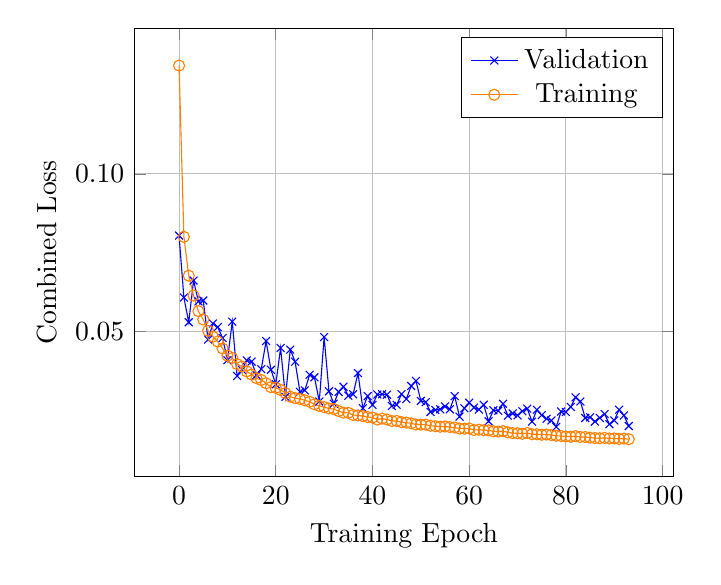
\begin{tikzpicture}
            \begin{axis}[
                    xlabel={Training Epoch},
                    ylabel={Combined Loss},
                    grid=major,
                    y tick label style={
                            /pgf/number format/.cd,
                            fixed,
                            fixed zerofill,
                            precision=2,
                            /tikz/.cd
                        },
                    x tick label style={
                            /pgf/number format/.cd,
                            fixed,
                            fixed zerofill,
                            precision=0,
                            /tikz/.cd
                        }
                ]

                \addplot [color=blue, mark=x] coordinates {
                        (0, 0.08043164759874344)
                        (1, 0.06074518710374832)
                        (2, 0.052902426570653915)
                        (3, 0.06613180786371231)
                        (4, 0.059524212032556534)
                        (5, 0.05979877710342407)
                        (6, 0.04741564020514488)
                        (7, 0.05249345675110817)
                        (8, 0.05137933790683746)
                        (9, 0.04790901765227318)
                        (10, 0.040847595781087875)
                        (11, 0.05307967960834503)
                        (12, 0.03584986925125122)
                        (13, 0.03778165951371193)
                        (14, 0.040794435888528824)
                        (15, 0.04041244089603424)
                        (16, 0.03612484037876129)
                        (17, 0.03802626579999924)
                        (18, 0.0469294972717762)
                        (19, 0.03780488297343254)
                        (20, 0.033201076090335846)
                        (21, 0.04474097117781639)
                        (22, 0.02922258898615837)
                        (23, 0.04421123117208481)
                        (24, 0.04037603363394737)
                        (25, 0.030803710222244263)
                        (26, 0.03126450628042221)
                        (27, 0.03620780631899834)
                        (28, 0.03541986271739006)
                        (29, 0.027726246044039726)
                        (30, 0.04819177836179733)
                        (31, 0.030984409153461456)
                        (32, 0.027061015367507935)
                        (33, 0.03080209530889988)
                        (34, 0.03243536502122879)
                        (35, 0.02956921048462391)
                        (36, 0.03002588078379631)
                        (37, 0.03678334876894951)
                        (38, 0.025607910007238388)
                        (39, 0.02945389598608017)
                        (40, 0.026652036234736443)
                        (41, 0.029962878674268723)
                        (42, 0.030048390850424767)
                        (43, 0.029896989464759827)
                        (44, 0.026323826983571053)
                        (45, 0.026708098128437996)
                        (46, 0.030077103525400162)
                        (47, 0.028525060042738914)
                        (48, 0.032686349004507065)
                        (49, 0.034263286739587784)
                        (50, 0.027927376329898834)
                        (51, 0.027547994628548622)
                        (52, 0.02441718429327011)
                        (53, 0.025028863921761513)
                        (54, 0.025253266096115112)
                        (55, 0.026195263490080833)
                        (56, 0.02525722235441208)
                        (57, 0.029447326436638832)
                        (58, 0.02292432077229023)
                        (59, 0.025586243718862534)
                        (60, 0.027354903519153595)
                        (61, 0.025817271322011948)
                        (62, 0.02517731487751007)
                        (63, 0.026702845469117165)
                        (64, 0.021456172689795494)
                        (65, 0.024942679330706596)
                        (66, 0.024776998907327652)
                        (67, 0.0270153246819973)
                        (68, 0.02322125807404518)
                        (69, 0.02393546886742115)
                        (70, 0.023330790922045708)
                        (71, 0.024663137272000313)
                        (72, 0.02549472078680992)
                        (73, 0.021344535052776337)
                        (74, 0.02510169893503189)
                        (75, 0.02341744862496853)
                        (76, 0.02226269245147705)
                        (77, 0.02173188142478466)
                        (78, 0.019678140059113503)
                        (79, 0.024568742141127586)
                        (80, 0.024419642984867096)
                        (81, 0.026015497744083405)
                        (82, 0.029056107625365257)
                        (83, 0.027733109891414642)
                        (84, 0.02249683439731598)
                        (85, 0.02272811532020569)
                        (86, 0.021356647834181786)
                        (87, 0.022520456463098526)
                        (88, 0.023762699216604233)
                        (89, 0.020549410954117775)
                        (90, 0.021727249026298523)
                        (91, 0.025129979476332664)
                        (92, 0.02330918423831463)
                        (93, 0.01995863765478134)
                    };
                \addlegendentry{Validation}
                \addplot [color=orange, mark=o] coordinates {
                        (0, 0.1343851387500763)
                        (1, 0.08002151548862457)
                        (2, 0.0676926001906395)
                        (3, 0.06139257550239563)
                        (4, 0.05642293021082878)
                        (5, 0.05375717580318451)
                        (6, 0.05020662397146225)
                        (7, 0.048321682959795)
                        (8, 0.04678958281874657)
                        (9, 0.04458630084991455)
                        (10, 0.04228425398468971)
                        (11, 0.04156023636460304)
                        (12, 0.03960949182510376)
                        (13, 0.03883389011025429)
                        (14, 0.03730262443423271)
                        (15, 0.03628617152571678)
                        (16, 0.035156965255737305)
                        (17, 0.03456437960267067)
                        (18, 0.033544786274433136)
                        (19, 0.03229551389813423)
                        (20, 0.032057005912065506)
                        (21, 0.03141874074935913)
                        (22, 0.030402392148971558)
                        (23, 0.029280880466103554)
                        (24, 0.028812170028686523)
                        (25, 0.02853376977145672)
                        (26, 0.028138507157564163)
                        (27, 0.02766536734998226)
                        (28, 0.026845796033740044)
                        (29, 0.026329142972826958)
                        (30, 0.025947747752070427)
                        (31, 0.025546777993440628)
                        (32, 0.02534446120262146)
                        (33, 0.02470041997730732)
                        (34, 0.02418896183371544)
                        (35, 0.024137726053595543)
                        (36, 0.023455774411559105)
                        (37, 0.02332555316388607)
                        (38, 0.02311769314110279)
                        (39, 0.02281922474503517)
                        (40, 0.022646227851510048)
                        (41, 0.022006521001458168)
                        (42, 0.02231583371758461)
                        (43, 0.0220238845795393)
                        (44, 0.02154807560145855)
                        (45, 0.021573565900325775)
                        (46, 0.021174723282456398)
                        (47, 0.021037429571151733)
                        (48, 0.02080686204135418)
                        (49, 0.02044449746608734)
                        (50, 0.020399533212184906)
                        (51, 0.020404336974024773)
                        (52, 0.020036347210407257)
                        (53, 0.019890690222382545)
                        (54, 0.01973242685198784)
                        (55, 0.019804585725069046)
                        (56, 0.019626755267381668)
                        (57, 0.019482489675283432)
                        (58, 0.019158650189638138)
                        (59, 0.019094763323664665)
                        (60, 0.019187889993190765)
                        (61, 0.018664531409740448)
                        (62, 0.018800128251314163)
                        (63, 0.018644247204065323)
                        (64, 0.01858060620725155)
                        (65, 0.018279019743204117)
                        (66, 0.01820104382932186)
                        (67, 0.018337523564696312)
                        (68, 0.01794120855629444)
                        (69, 0.017697131261229515)
                        (70, 0.01766018010675907)
                        (71, 0.017467152327299118)
                        (72, 0.017742985859513283)
                        (73, 0.017354626208543777)
                        (74, 0.01734267920255661)
                        (75, 0.017183884978294373)
                        (76, 0.01725749485194683)
                        (77, 0.01709301955997944)
                        (78, 0.016869720071554184)
                        (79, 0.016784045845270157)
                        (80, 0.016648223623633385)
                        (81, 0.016545940190553665)
                        (82, 0.016758624464273453)
                        (83, 0.016489233821630478)
                        (84, 0.016458027064800262)
                        (85, 0.016275009140372276)
                        (86, 0.016141092404723167)
                        (87, 0.016066214069724083)
                        (88, 0.016197066754102707)
                        (89, 0.016004158183932304)
                        (90, 0.0160329882055521)
                        (91, 0.015863537788391113)
                        (92, 0.015965698286890984)
                        (93, 0.015778299421072006)
                    };
                \addlegendentry{Training}
            \end{axis}
        \end{tikzpicture}
        \caption{Combined loss over Epochs}
        \label{fig:lossrcae2D1D}
    \end{subfigure}
    \hfill
    \begin{subfigure}{0.45\textwidth}
        \centering
        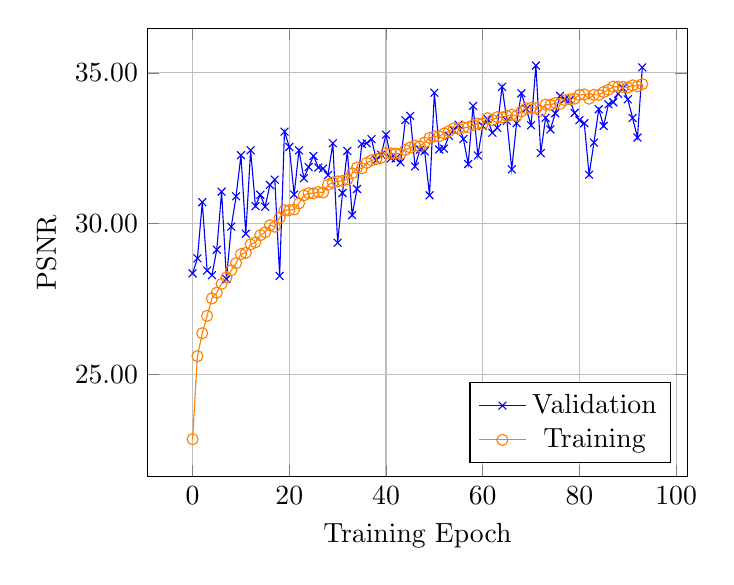
\begin{tikzpicture}
            \begin{axis}[
                    legend pos = south east,
                    xlabel={Training Epoch},
                    ylabel={PSNR},
                    grid=major,
                    y tick label style={
                            /pgf/number format/.cd,
                            fixed,
                            fixed zerofill,
                            precision=2,
                            /tikz/.cd
                        },
                    x tick label style={
                            /pgf/number format/.cd,
                            fixed,
                            fixed zerofill,
                            precision=0,
                            /tikz/.cd
                        }
                ]

                \addplot [color=blue, mark=x] coordinates {
                        (0, 28.344541549682617)
                        (1, 28.84223175048828)
                        (2, 30.705745697021484)
                        (3, 28.437992095947266)
                        (4, 28.28574562072754)
                        (5, 29.12853240966797)
                        (6, 31.05563735961914)
                        (7, 28.15410041809082)
                        (8, 29.897279739379883)
                        (9, 30.902278900146484)
                        (10, 32.26592254638672)
                        (11, 29.6603946685791)
                        (12, 32.428226470947266)
                        (13, 30.57418441772461)
                        (14, 30.95284652709961)
                        (15, 30.55739974975586)
                        (16, 31.277748107910156)
                        (17, 31.45418930053711)
                        (18, 28.25841522216797)
                        (19, 33.047889709472656)
                        (20, 32.540340423583984)
                        (21, 30.960424423217773)
                        (22, 32.42625045776367)
                        (23, 31.501789093017578)
                        (24, 31.87565040588379)
                        (25, 32.24083709716797)
                        (26, 31.856706619262695)
                        (27, 31.823551177978516)
                        (28, 31.606935501098633)
                        (29, 32.66322708129883)
                        (30, 29.358972549438477)
                        (31, 31.011899948120117)
                        (32, 32.408164978027344)
                        (33, 30.277769088745117)
                        (34, 31.143646240234375)
                        (35, 32.64175796508789)
                        (36, 32.66264724731445)
                        (37, 32.798274993896484)
                        (38, 32.10250473022461)
                        (39, 32.28035354614258)
                        (40, 32.949989318847656)
                        (41, 32.16492462158203)
                        (42, 32.15773391723633)
                        (43, 32.02846145629883)
                        (44, 33.42640686035156)
                        (45, 33.57099151611328)
                        (46, 31.894275665283203)
                        (47, 32.44635009765625)
                        (48, 32.396728515625)
                        (49, 30.934661865234375)
                        (50, 34.340126037597656)
                        (51, 32.45600509643555)
                        (52, 32.48563003540039)
                        (53, 32.91167068481445)
                        (54, 33.09199142456055)
                        (55, 33.28013229370117)
                        (56, 32.80531311035156)
                        (57, 31.971961975097656)
                        (58, 33.90090560913086)
                        (59, 32.25581359863281)
                        (60, 33.23826599121094)
                        (61, 33.46126937866211)
                        (62, 33.00965881347656)
                        (63, 33.17349624633789)
                        (64, 34.53411102294922)
                        (65, 33.409751892089844)
                        (66, 31.79792022705078)
                        (67, 33.32783889770508)
                        (68, 34.31901550292969)
                        (69, 33.80420684814453)
                        (70, 33.260379791259766)
                        (71, 35.240238189697266)
                        (72, 32.33718490600586)
                        (73, 33.50505447387695)
                        (74, 33.120826721191406)
                        (75, 33.657840728759766)
                        (76, 34.23663330078125)
                        (77, 34.12425231933594)
                        (78, 34.09874725341797)
                        (79, 33.669315338134766)
                        (80, 33.42665481567383)
                        (81, 33.327877044677734)
                        (82, 31.615806579589844)
                        (83, 32.68410873413086)
                        (84, 33.792118072509766)
                        (85, 33.23866271972656)
                        (86, 33.95402145385742)
                        (87, 34.0231819152832)
                        (88, 34.30799102783203)
                        (89, 34.49597930908203)
                        (90, 34.12025833129883)
                        (91, 33.501033782958984)
                        (92, 32.852115631103516)
                        (93, 35.180240631103516)
                    };
                \addlegendentry{Validation}
                \addplot [color=orange, mark=o] coordinates {
                        (0, 22.840473175048828)
                        (1, 25.59564208984375)
                        (2, 26.35555648803711)
                        (3, 26.93279457092285)
                        (4, 27.512571334838867)
                        (5, 27.70417594909668)
                        (6, 27.997432708740234)
                        (7, 28.211559295654297)
                        (8, 28.447351455688477)
                        (9, 28.68265724182129)
                        (10, 28.981760025024414)
                        (11, 29.023277282714844)
                        (12, 29.30708885192871)
                        (13, 29.374794006347656)
                        (14, 29.611570358276367)
                        (15, 29.70522117614746)
                        (16, 29.940519332885742)
                        (17, 29.89218521118164)
                        (18, 30.189586639404297)
                        (19, 30.43790626525879)
                        (20, 30.44263458251953)
                        (21, 30.461393356323242)
                        (22, 30.66482162475586)
                        (23, 30.933631896972656)
                        (24, 31.00392723083496)
                        (25, 30.99812889099121)
                        (26, 31.043848037719727)
                        (27, 31.02802848815918)
                        (28, 31.280405044555664)
                        (29, 31.356891632080078)
                        (30, 31.3989200592041)
                        (31, 31.415361404418945)
                        (32, 31.461576461791992)
                        (33, 31.665390014648438)
                        (34, 31.851123809814453)
                        (35, 31.828380584716797)
                        (36, 32.00942611694336)
                        (37, 32.09245681762695)
                        (38, 32.13841247558594)
                        (39, 32.18345642089844)
                        (40, 32.338687896728516)
                        (41, 32.32752990722656)
                        (42, 32.31797409057617)
                        (43, 32.310909271240234)
                        (44, 32.44256591796875)
                        (45, 32.52096939086914)
                        (46, 32.58245086669922)
                        (47, 32.55992126464844)
                        (48, 32.68859100341797)
                        (49, 32.83682632446289)
                        (50, 32.89097595214844)
                        (51, 32.893680572509766)
                        (52, 32.9880485534668)
                        (53, 33.06246566772461)
                        (54, 33.15457534790039)
                        (55, 33.1440544128418)
                        (56, 33.18609619140625)
                        (57, 33.19806671142578)
                        (58, 33.26390075683594)
                        (59, 33.314937591552734)
                        (60, 33.31688690185547)
                        (61, 33.49351501464844)
                        (62, 33.43267822265625)
                        (63, 33.5284309387207)
                        (64, 33.52117919921875)
                        (65, 33.56513214111328)
                        (66, 33.61211395263672)
                        (67, 33.57004928588867)
                        (68, 33.718475341796875)
                        (69, 33.824398040771484)
                        (70, 33.83839797973633)
                        (71, 33.82554244995117)
                        (72, 33.73871612548828)
                        (73, 33.946319580078125)
                        (74, 33.93394088745117)
                        (75, 33.99967956542969)
                        (76, 33.973392486572266)
                        (77, 34.09053421020508)
                        (78, 34.11981964111328)
                        (79, 34.143741607666016)
                        (80, 34.266544342041016)
                        (81, 34.28181838989258)
                        (82, 34.14168930053711)
                        (83, 34.271305084228516)
                        (84, 34.26491928100586)
                        (85, 34.36074447631836)
                        (86, 34.438385009765625)
                        (87, 34.54080581665039)
                        (88, 34.533573150634766)
                        (89, 34.53550720214844)
                        (90, 34.51221466064453)
                        (91, 34.58344268798828)
                        (92, 34.550804138183594)
                        (93, 34.62499237060547)
                    };
                \addlegendentry{Training}
            \end{axis}
        \end{tikzpicture}
        \caption{PSNR over Epochs}
        \label{fig:psnrcae2D1D}
    \end{subfigure}

    \begin{subfigure}{0.45\textwidth}
        \centering
        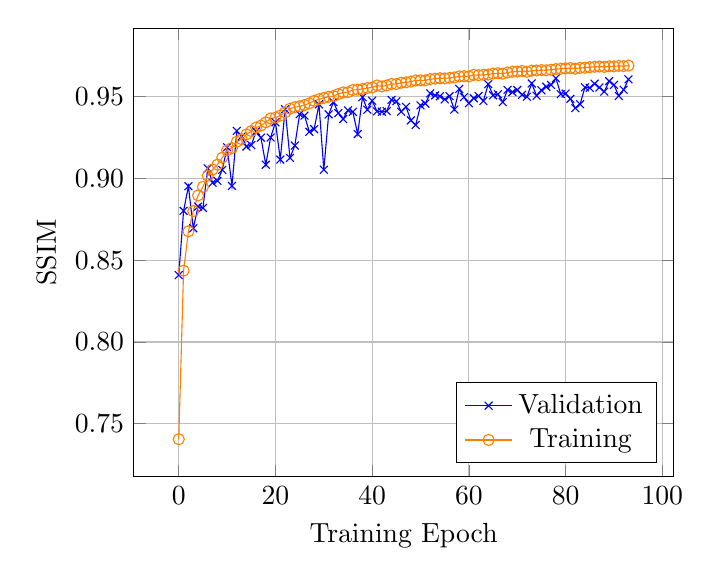
\begin{tikzpicture}
            \begin{axis}[
                    legend pos = south east,
                    xlabel={Training Epoch},
                    ylabel={SSIM},
                    grid=major,
                    y tick label style={
                            /pgf/number format/.cd,
                            fixed,
                            fixed zerofill,
                            precision=2,
                            /tikz/.cd
                        },
                    x tick label style={
                            /pgf/number format/.cd,
                            fixed,
                            fixed zerofill,
                            precision=0,
                            /tikz/.cd
                        }
                ]

                \addplot [color=blue, mark=x] coordinates {
                        (0, 0.8408826589584351)
                        (1, 0.8801040053367615)
                        (2, 0.8951815962791443)
                        (3, 0.869461715221405)
                        (4, 0.8827323317527771)
                        (5, 0.8818970918655396)
                        (6, 0.906104326248169)
                        (7, 0.8972965478897095)
                        (8, 0.8984814286231995)
                        (9, 0.9051082730293274)
                        (10, 0.9189834594726562)
                        (11, 0.8953373432159424)
                        (12, 0.9289712309837341)
                        (13, 0.9255644083023071)
                        (14, 0.9194149971008301)
                        (15, 0.9202849864959717)
                        (16, 0.92868572473526)
                        (17, 0.92481529712677)
                        (18, 0.9082924723625183)
                        (19, 0.9249349236488342)
                        (20, 0.9342451691627502)
                        (21, 0.9114547967910767)
                        (22, 0.9422348141670227)
                        (23, 0.9124616384506226)
                        (24, 0.9200233221054077)
                        (25, 0.9391650557518005)
                        (26, 0.9382834434509277)
                        (27, 0.9284080862998962)
                        (28, 0.9300312995910645)
                        (29, 0.9452160596847534)
                        (30, 0.9052197337150574)
                        (31, 0.9390354752540588)
                        (32, 0.9466026425361633)
                        (33, 0.9398378133773804)
                        (34, 0.9361976385116577)
                        (35, 0.941486120223999)
                        (36, 0.9406081438064575)
                        (37, 0.9270246028900146)
                        (38, 0.9495564699172974)
                        (39, 0.9419049620628357)
                        (40, 0.9473863244056702)
                        (41, 0.9408657550811768)
                        (42, 0.940684974193573)
                        (43, 0.9410479068756104)
                        (44, 0.9479295611381531)
                        (45, 0.9471235871315002)
                        (46, 0.9406803250312805)
                        (47, 0.9436807036399841)
                        (48, 0.9353864192962646)
                        (49, 0.9325733780860901)
                        (50, 0.944567859172821)
                        (51, 0.9456464648246765)
                        (52, 0.9518896341323853)
                        (53, 0.9506298899650574)
                        (54, 0.9501030445098877)
                        (55, 0.9481987953186035)
                        (56, 0.950178325176239)
                        (57, 0.9419956803321838)
                        (58, 0.9546644687652588)
                        (59, 0.949592113494873)
                        (60, 0.9459035992622375)
                        (61, 0.9489359259605408)
                        (62, 0.950336217880249)
                        (63, 0.94722980260849)
                        (64, 0.9575068950653076)
                        (65, 0.950713038444519)
                        (66, 0.951390266418457)
                        (67, 0.9465607404708862)
                        (68, 0.9540260434150696)
                        (69, 0.9526825547218323)
                        (70, 0.9539524912834167)
                        (71, 0.9510356783866882)
                        (72, 0.9498273134231567)
                        (73, 0.9579459428787231)
                        (74, 0.9504690170288086)
                        (75, 0.9537636637687683)
                        (76, 0.9559479355812073)
                        (77, 0.9570521712303162)
                        (78, 0.9611473083496094)
                        (79, 0.9514384269714355)
                        (80, 0.9517682790756226)
                        (81, 0.948560357093811)
                        (82, 0.942854106426239)
                        (83, 0.9453123807907104)
                        (84, 0.9555776715278625)
                        (85, 0.9552397727966309)
                        (86, 0.9578328132629395)
                        (87, 0.9554721117019653)
                        (88, 0.9529644250869751)
                        (89, 0.9593670964241028)
                        (90, 0.957080602645874)
                        (91, 0.950336217880249)
                        (92, 0.9540977478027344)
                        (93, 0.9604547619819641)
                    };
                \addlegendentry{Validation}
                \addplot [color=orange, mark=o] coordinates {
                        (0, 0.7405810356140137)
                        (1, 0.8435698747634888)
                        (2, 0.8676023483276367)
                        (3, 0.8799480199813843)
                        (4, 0.8895593881607056)
                        (5, 0.8947440385818481)
                        (6, 0.9016340374946594)
                        (7, 0.9053784012794495)
                        (8, 0.9083206653594971)
                        (9, 0.9126300811767578)
                        (10, 0.9170833826065063)
                        (11, 0.9185397624969482)
                        (12, 0.9223192930221558)
                        (13, 0.9239017963409424)
                        (14, 0.9268496036529541)
                        (15, 0.9288532137870789)
                        (16, 0.931037962436676)
                        (17, 0.9322584867477417)
                        (18, 0.9341848492622375)
                        (19, 0.9365788102149963)
                        (20, 0.9371162056922913)
                        (21, 0.9383733868598938)
                        (22, 0.9403270483016968)
                        (23, 0.9425204992294312)
                        (24, 0.9434581398963928)
                        (25, 0.9439932107925415)
                        (26, 0.9447728395462036)
                        (27, 0.9457909464836121)
                        (28, 0.9473243951797485)
                        (29, 0.9483187198638916)
                        (30, 0.9490971565246582)
                        (31, 0.9498494863510132)
                        (32, 0.9502743482589722)
                        (33, 0.9514946341514587)
                        (34, 0.9524883031845093)
                        (35, 0.9526179432868958)
                        (36, 0.9539328217506409)
                        (37, 0.9541752338409424)
                        (38, 0.9545777440071106)
                        (39, 0.955173134803772)
                        (40, 0.9555010795593262)
                        (41, 0.9567475914955139)
                        (42, 0.956150472164154)
                        (43, 0.9567326903343201)
                        (44, 0.9576536417007446)
                        (45, 0.9575949907302856)
                        (46, 0.9583911299705505)
                        (47, 0.9586556553840637)
                        (48, 0.9590813517570496)
                        (49, 0.9597735404968262)
                        (50, 0.9598850011825562)
                        (51, 0.9598568081855774)
                        (52, 0.9605821371078491)
                        (53, 0.9608520865440369)
                        (54, 0.9611578583717346)
                        (55, 0.9610406160354614)
                        (56, 0.9613662362098694)
                        (57, 0.9616594314575195)
                        (58, 0.9622913599014282)
                        (59, 0.9624056220054626)
                        (60, 0.9622215032577515)
                        (61, 0.963238000869751)
                        (62, 0.9629802107810974)
                        (63, 0.963269829750061)
                        (64, 0.9634012579917908)
                        (65, 0.9640065431594849)
                        (66, 0.9641762971878052)
                        (67, 0.9639100432395935)
                        (68, 0.9646515846252441)
                        (69, 0.9651387929916382)
                        (70, 0.9652068018913269)
                        (71, 0.9655851721763611)
                        (72, 0.9650793075561523)
                        (73, 0.9657989740371704)
                        (74, 0.9658368825912476)
                        (75, 0.9661278128623962)
                        (76, 0.966001033782959)
                        (77, 0.9663295745849609)
                        (78, 0.9667510986328125)
                        (79, 0.9669081568717957)
                        (80, 0.9671602249145508)
                        (81, 0.9673614501953125)
                        (82, 0.9669657349586487)
                        (83, 0.9674848914146423)
                        (84, 0.9675517082214355)
                        (85, 0.9679052829742432)
                        (86, 0.9681609272956848)
                        (87, 0.9682982563972473)
                        (88, 0.9680608510971069)
                        (89, 0.9684416055679321)
                        (90, 0.9683763384819031)
                        (91, 0.9687038064002991)
                        (92, 0.9685118794441223)
                        (93, 0.9688760638237)
                    };
                \addlegendentry{Training}
            \end{axis}
        \end{tikzpicture}
        \caption{SSIM over Epochs}
        \label{fig:ssimrcae2D1D}
    \end{subfigure}
    \hfill
    \begin{subfigure}{0.45\textwidth}
        \centering
        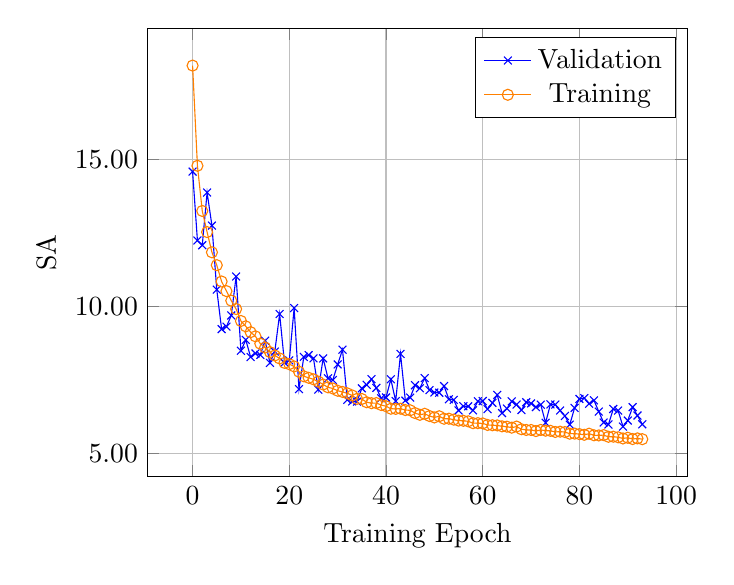
\begin{tikzpicture}
            \begin{axis}[
                    xlabel={Training Epoch},
                    ylabel={SA},
                    grid=major,
                    y tick label style={
                            /pgf/number format/.cd,
                            fixed,
                            fixed zerofill,
                            precision=2,
                            /tikz/.cd
                        },
                    x tick label style={
                            /pgf/number format/.cd,
                            fixed,
                            fixed zerofill,
                            precision=0,
                            /tikz/.cd
                        }
                ]

                \addplot [color=blue, mark=x] coordinates {
                        (0, 14.581341743469238)
                        (1, 12.236696243286133)
                        (2, 12.075876235961914)
                        (3, 13.8683443069458)
                        (4, 12.744482040405273)
                        (5, 10.564677238464355)
                        (6, 9.221210479736328)
                        (7, 9.305386543273926)
                        (8, 9.685998916625977)
                        (9, 11.012198448181152)
                        (10, 8.485595703125)
                        (11, 8.856318473815918)
                        (12, 8.271440505981445)
                        (13, 8.392439842224121)
                        (14, 8.343060493469238)
                        (15, 8.828171730041504)
                        (16, 8.071915626525879)
                        (17, 8.457357406616211)
                        (18, 9.734896659851074)
                        (19, 8.081356048583984)
                        (20, 8.157341003417969)
                        (21, 9.937481880187988)
                        (22, 7.179562568664551)
                        (23, 8.277581214904785)
                        (24, 8.338167190551758)
                        (25, 8.226338386535645)
                        (26, 7.163015365600586)
                        (27, 8.225053787231445)
                        (28, 7.547837257385254)
                        (29, 7.49119234085083)
                        (30, 8.019854545593262)
                        (31, 8.521427154541016)
                        (32, 6.815619945526123)
                        (33, 6.7626566886901855)
                        (34, 6.755538463592529)
                        (35, 7.207146167755127)
                        (36, 7.327016353607178)
                        (37, 7.520761966705322)
                        (38, 7.221956253051758)
                        (39, 6.869656562805176)
                        (40, 6.8946075439453125)
                        (41, 7.515515327453613)
                        (42, 6.771356582641602)
                        (43, 8.377212524414062)
                        (44, 6.789178848266602)
                        (45, 6.891229629516602)
                        (46, 7.3121538162231445)
                        (47, 7.211207866668701)
                        (48, 7.554929256439209)
                        (49, 7.144186019897461)
                        (50, 7.0652031898498535)
                        (51, 7.056988716125488)
                        (52, 7.284759998321533)
                        (53, 6.833992004394531)
                        (54, 6.81394624710083)
                        (55, 6.454461574554443)
                        (56, 6.599137783050537)
                        (57, 6.595466613769531)
                        (58, 6.457442760467529)
                        (59, 6.766847610473633)
                        (60, 6.774369716644287)
                        (61, 6.498928070068359)
                        (62, 6.710445880889893)
                        (63, 6.984724521636963)
                        (64, 6.364790916442871)
                        (65, 6.518082141876221)
                        (66, 6.765005588531494)
                        (67, 6.655009746551514)
                        (68, 6.467051029205322)
                        (69, 6.7331390380859375)
                        (70, 6.693365097045898)
                        (71, 6.568737030029297)
                        (72, 6.649855613708496)
                        (73, 6.035009384155273)
                        (74, 6.6612677574157715)
                        (75, 6.654373645782471)
                        (76, 6.45399284362793)
                        (77, 6.266611576080322)
                        (78, 5.970256328582764)
                        (79, 6.541666507720947)
                        (80, 6.847097873687744)
                        (81, 6.875332832336426)
                        (82, 6.6838483810424805)
                        (83, 6.796766757965088)
                        (84, 6.415521621704102)
                        (85, 6.043882846832275)
                        (86, 5.976872444152832)
                        (87, 6.5049333572387695)
                        (88, 6.449991703033447)
                        (89, 5.905304431915283)
                        (90, 6.110677719116211)
                        (91, 6.567947864532471)
                        (92, 6.281253337860107)
                        (93, 5.9842529296875)
                    };
                \addlegendentry{Validation}
                \addplot [color=orange, mark=o] coordinates {
                        (0, 18.187992095947266)
                        (1, 14.779180526733398)
                        (2, 13.241893768310547)
                        (3, 12.522732734680176)
                        (4, 11.83489990234375)
                        (5, 11.39739990234375)
                        (6, 10.842321395874023)
                        (7, 10.514589309692383)
                        (8, 10.189064979553223)
                        (9, 9.904563903808594)
                        (10, 9.498167037963867)
                        (11, 9.316301345825195)
                        (12, 9.117477416992188)
                        (13, 8.976700782775879)
                        (14, 8.72721004486084)
                        (15, 8.59417724609375)
                        (16, 8.43934440612793)
                        (17, 8.32339096069336)
                        (18, 8.224353790283203)
                        (19, 8.073709487915039)
                        (20, 8.027946472167969)
                        (21, 7.951269149780273)
                        (22, 7.772907257080078)
                        (23, 7.616519451141357)
                        (24, 7.565118789672852)
                        (25, 7.513928413391113)
                        (26, 7.434066295623779)
                        (27, 7.336695194244385)
                        (28, 7.240935325622559)
                        (29, 7.202029705047607)
                        (30, 7.124884605407715)
                        (31, 7.084807395935059)
                        (32, 7.036352157592773)
                        (33, 6.965587139129639)
                        (34, 6.848552227020264)
                        (35, 6.843993186950684)
                        (36, 6.733633041381836)
                        (37, 6.701430320739746)
                        (38, 6.70559549331665)
                        (39, 6.639238357543945)
                        (40, 6.598560810089111)
                        (41, 6.513266086578369)
                        (42, 6.5077290534973145)
                        (43, 6.515286922454834)
                        (44, 6.467470169067383)
                        (45, 6.459924697875977)
                        (46, 6.365881443023682)
                        (47, 6.306219100952148)
                        (48, 6.3405022621154785)
                        (49, 6.263949394226074)
                        (50, 6.217156410217285)
                        (51, 6.257030963897705)
                        (52, 6.172695636749268)
                        (53, 6.17436408996582)
                        (54, 6.142100811004639)
                        (55, 6.1084675788879395)
                        (56, 6.102687358856201)
                        (57, 6.08415412902832)
                        (58, 6.021203994750977)
                        (59, 6.022428035736084)
                        (60, 6.013216495513916)
                        (61, 5.960674285888672)
                        (62, 5.950702667236328)
                        (63, 5.945780277252197)
                        (64, 5.913205146789551)
                        (65, 5.903091907501221)
                        (66, 5.8684892654418945)
                        (67, 5.905476093292236)
                        (68, 5.81553316116333)
                        (69, 5.7908711433410645)
                        (70, 5.789422988891602)
                        (71, 5.751892566680908)
                        (72, 5.791591644287109)
                        (73, 5.765942096710205)
                        (74, 5.760958671569824)
                        (75, 5.723372459411621)
                        (76, 5.733331203460693)
                        (77, 5.719126224517822)
                        (78, 5.663020133972168)
                        (79, 5.6667938232421875)
                        (80, 5.6486663818359375)
                        (81, 5.625856876373291)
                        (82, 5.662928104400635)
                        (83, 5.610086917877197)
                        (84, 5.604851245880127)
                        (85, 5.615926742553711)
                        (86, 5.558119297027588)
                        (87, 5.561817169189453)
                        (88, 5.541243553161621)
                        (89, 5.501564025878906)
                        (90, 5.525884628295898)
                        (91, 5.48138952255249)
                        (92, 5.504373073577881)
                        (93, 5.476596832275391)
                    };
                \addlegendentry{Training}
            \end{axis}
        \end{tikzpicture}
        \caption{Spectral Angle over Epochs}
        \label{fig:sarcae2D1D}
    \end{subfigure}

    \begin{subfigure}{0.45\textwidth}
        \centering
        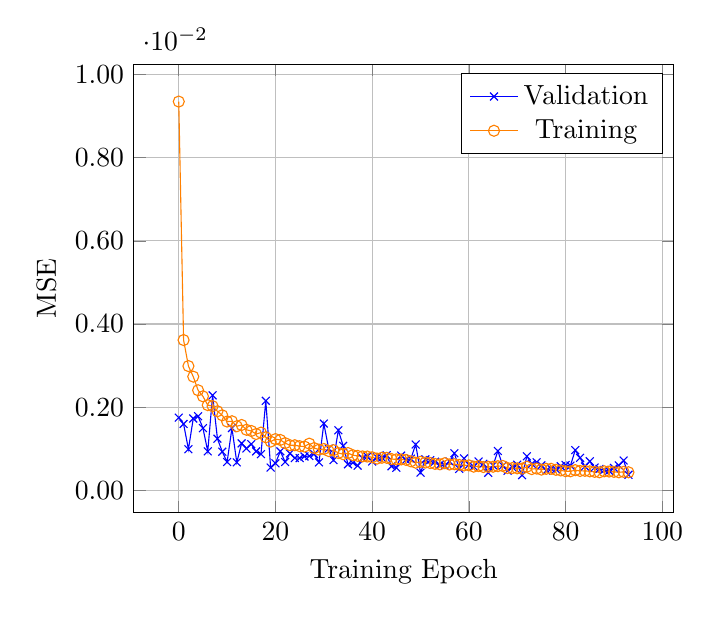
\begin{tikzpicture}
            \begin{axis}[
                    xlabel={Training Epoch},
                    ylabel={MSE},
                    grid=major,
                    y tick label style={
                            /pgf/number format/.cd,
                            fixed,
                            fixed zerofill,
                            precision=2,
                            /tikz/.cd
                        },
                    x tick label style={
                            /pgf/number format/.cd,
                            fixed,
                            fixed zerofill,
                            precision=0,
                            /tikz/.cd
                        }
                ]

                \addplot [color=blue, mark=x] coordinates {
                        (0, 0.0017457511276006699)
                        (1, 0.0015947317006066442)
                        (2, 0.0009863856248557568)
                        (3, 0.0017252841498702765)
                        (4, 0.0017804153030738235)
                        (5, 0.0014945084694772959)
                        (6, 0.0009355253423564136)
                        (7, 0.002283069072291255)
                        (8, 0.001240077312104404)
                        (9, 0.0009262083913199604)
                        (10, 0.0006783897988498211)
                        (11, 0.001496345386840403)
                        (12, 0.0006705613923259079)
                        (13, 0.0011277050944045186)
                        (14, 0.0010036969324573874)
                        (15, 0.0011091590858995914)
                        (16, 0.0009351182961836457)
                        (17, 0.0008680409519001842)
                        (18, 0.002151512075215578)
                        (19, 0.0005448232404887676)
                        (20, 0.0006478155264630914)
                        (21, 0.0009368881583213806)
                        (22, 0.0006799548282288015)
                        (23, 0.000883894506841898)
                        (24, 0.0007751567172817886)
                        (25, 0.0007731161313131452)
                        (26, 0.0008120362181216478)
                        (27, 0.000823481532279402)
                        (28, 0.0008714239811524749)
                        (29, 0.0006688698194921017)
                        (30, 0.0016030450351536274)
                        (31, 0.0010040714405477047)
                        (32, 0.0007244457374326885)
                        (33, 0.001442230655811727)
                        (34, 0.001068652025423944)
                        (35, 0.0006244503310881555)
                        (36, 0.000660331454128027)
                        (37, 0.0005915058427490294)
                        (38, 0.0007725028553977609)
                        (39, 0.0008131882641464472)
                        (40, 0.0006902554887346923)
                        (41, 0.0007908859988674521)
                        (42, 0.0007816083962097764)
                        (43, 0.0008420139201916754)
                        (44, 0.0005767563707195222)
                        (45, 0.0005400183144956827)
                        (46, 0.0008339302148669958)
                        (47, 0.000730833038687706)
                        (48, 0.0007587698637507856)
                        (49, 0.0011004272382706404)
                        (50, 0.0004228340112604201)
                        (51, 0.0007427572854794562)
                        (52, 0.000724111101590097)
                        (53, 0.0006872070953249931)
                        (54, 0.0006091073155403137)
                        (55, 0.0005892133922316134)
                        (56, 0.000692586530931294)
                        (57, 0.000890478549990803)
                        (58, 0.0005130190984345973)
                        (59, 0.0007644309080205858)
                        (60, 0.0006133205606602132)
                        (61, 0.0005701599875465035)
                        (62, 0.0006909333751536906)
                        (63, 0.0006358209648169577)
                        (64, 0.0004192522319499403)
                        (65, 0.0005987282493151724)
                        (66, 0.0009439693531021476)
                        (67, 0.0005917109083384275)
                        (68, 0.00046838700654916465)
                        (69, 0.0005532176000997424)
                        (70, 0.0006138001335784793)
                        (71, 0.00036207519588060677)
                        (72, 0.0008166736224666238)
                        (73, 0.0006349689210765064)
                        (74, 0.0006722445250488818)
                        (75, 0.0005982734146527946)
                        (76, 0.00047323585022240877)
                        (77, 0.0005162435700185597)
                        (78, 0.0005039831157773733)
                        (79, 0.0005763505469076335)
                        (80, 0.0006075954879634082)
                        (81, 0.0005914527573622763)
                        (82, 0.0009659489151090384)
                        (83, 0.0007789601804688573)
                        (84, 0.0005719894543290138)
                        (85, 0.0006960093160159886)
                        (86, 0.0005462058470584452)
                        (87, 0.0005133844097144902)
                        (88, 0.0004895061138086021)
                        (89, 0.00046639202628284693)
                        (90, 0.0005353285814635456)
                        (91, 0.0005962393479421735)
                        (92, 0.0007160112727433443)
                        (93, 0.0003718939842656255)
                    };
                \addlegendentry{Validation}
                \addplot [color=orange, mark=o] coordinates {
                        (0, 0.009350764565169811)
                        (1, 0.003612789325416088)
                        (2, 0.0029868585988879204)
                        (3, 0.002732774941250682)
                        (4, 0.002404938917607069)
                        (5, 0.002258876571431756)
                        (6, 0.0020471892785280943)
                        (7, 0.0020221625454723835)
                        (8, 0.0018997741863131523)
                        (9, 0.0018024030141532421)
                        (10, 0.001651907921768725)
                        (11, 0.0016592844622209668)
                        (12, 0.0015389630571007729)
                        (13, 0.0015692723682150245)
                        (14, 0.0014545723097398877)
                        (15, 0.0014256919967010617)
                        (16, 0.0013526916736736894)
                        (17, 0.0013862026389688253)
                        (18, 0.0012743459083139896)
                        (19, 0.0011698162415996194)
                        (20, 0.001229880377650261)
                        (21, 0.0012098370352759957)
                        (22, 0.001133185112848878)
                        (23, 0.001081950729712844)
                        (24, 0.0010823486372828484)
                        (25, 0.0010597696527838707)
                        (26, 0.0010500333737581968)
                        (27, 0.001120819360949099)
                        (28, 0.0010143052786588669)
                        (29, 0.00097711943089962)
                        (30, 0.000991947017610073)
                        (31, 0.0009427490294910967)
                        (32, 0.0009630269487388432)
                        (33, 0.0008955372031778097)
                        (34, 0.0008665596833452582)
                        (35, 0.0008938608807511628)
                        (36, 0.0008434707415290177)
                        (37, 0.0008262331830337644)
                        (38, 0.0008138851262629032)
                        (39, 0.000811046629678458)
                        (40, 0.0007929778075776994)
                        (41, 0.0007601652760058641)
                        (42, 0.0007814798736944795)
                        (43, 0.0007798546575941145)
                        (44, 0.0007493983721360564)
                        (45, 0.0007421034388244152)
                        (46, 0.0007407969096675515)
                        (47, 0.0007298034033738077)
                        (48, 0.0006944446358829737)
                        (49, 0.0006621388019993901)
                        (50, 0.0006830905913375318)
                        (51, 0.000665608502458781)
                        (52, 0.0006545717478729784)
                        (53, 0.0006335502839647233)
                        (54, 0.0006224384997040033)
                        (55, 0.0006501759635284543)
                        (56, 0.0006196463364176452)
                        (57, 0.0006249911966733634)
                        (58, 0.0006091773975640535)
                        (59, 0.0005960640264675021)
                        (60, 0.0005984795279800892)
                        (61, 0.000566661125048995)
                        (62, 0.0005803650710731745)
                        (63, 0.0005586048355326056)
                        (64, 0.0005626806523650885)
                        (65, 0.0005649955710396171)
                        (66, 0.0005786537658423185)
                        (67, 0.0005843849503435194)
                        (68, 0.0005346994730643928)
                        (69, 0.0005325966631062329)
                        (70, 0.0005266342777758837)
                        (71, 0.0005195321864448488)
                        (72, 0.0005651357350870967)
                        (73, 0.0005080157425254583)
                        (74, 0.0005216559511609375)
                        (75, 0.0004953243187628686)
                        (76, 0.0005148557247593999)
                        (77, 0.0005149462958797812)
                        (78, 0.0004901767824776471)
                        (79, 0.0004761309828609228)
                        (80, 0.00045727050746791065)
                        (81, 0.00045418995432555676)
                        (82, 0.0004832110716961324)
                        (83, 0.0004631862975656986)
                        (84, 0.00046721327817067504)
                        (85, 0.00045369158033281565)
                        (86, 0.000441823125584051)
                        (87, 0.0004304925096221268)
                        (88, 0.0004549203149508685)
                        (89, 0.0004493097076192498)
                        (90, 0.0004415409348439425)
                        (91, 0.0004308459465391934)
                        (92, 0.0004419336037244648)
                        (93, 0.00043254243792034686)
                    };
                \addlegendentry{Training}
            \end{axis}
        \end{tikzpicture}
        \caption{MSE over Epochs}
        \label{fig:msercae2D1D}
    \end{subfigure}
    \caption{Training and Validation Metrics over Epochs for RCA2D1D}
    \label{fig:training_metricsrcae2D1D}


\end{figure}

\begin{figure}[h]
    \centering

    % ================= ENCODER =================
    \begin{minipage}{0.48\linewidth}
        \centering
        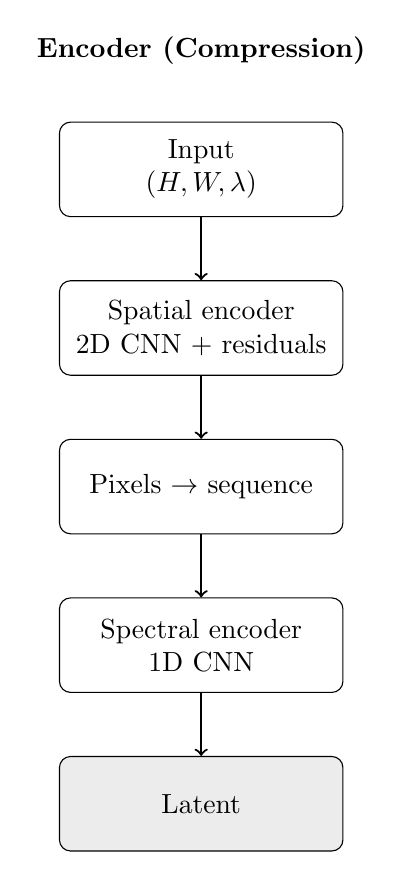
\begin{tikzpicture}[
                block/.style={draw, rounded corners, minimum width=3.6cm, minimum height=1.2cm, align=center},
                latent/.style={draw, rounded corners, minimum width=3.6cm, minimum height=1.2cm, align=center, fill=gray!15},
                arrow/.style={->, thick},
                node distance=0.8cm
            ]

            \node[block] (input) {Input\\$(H,W,\lambda)$};
            \node[block, below=of input] (spenc) {Spatial encoder\\2D CNN + residuals};
            \node[block, below=of spenc] (reshape1) {Pixels $\rightarrow$ sequence};
            \node[block, below=of reshape1] (specenc) {Spectral encoder\\1D CNN};
            \node[latent, below=of specenc] (latent) {Latent};

            \draw[arrow] (input) -- (spenc);
            \draw[arrow] (spenc) -- (reshape1);
            \draw[arrow] (reshape1) -- (specenc);
            \draw[arrow] (specenc) -- (latent);

            \node[above=0.6cm of input] {\textbf{Encoder (Compression)}};

        \end{tikzpicture}
    \end{minipage}
    \hfill
    % ================= DECODER =================
    \begin{minipage}{0.48\linewidth}
        \centering
        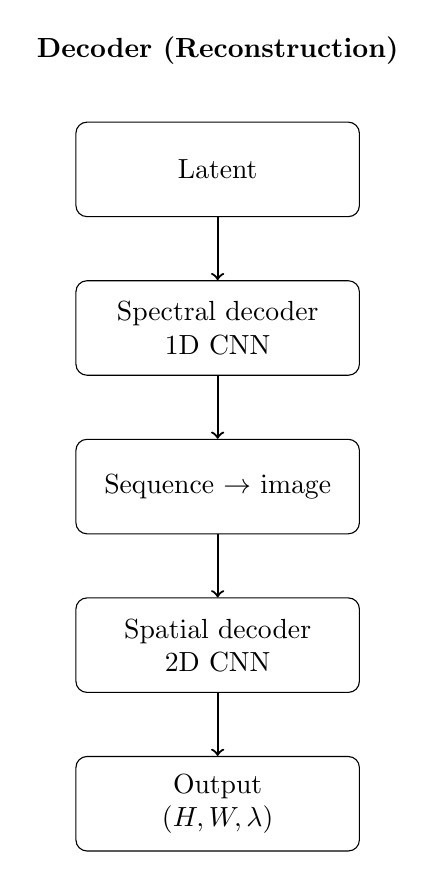
\begin{tikzpicture}[
                block/.style={draw, rounded corners, minimum width=3.6cm, minimum height=1.2cm, align=center},
                arrow/.style={->, thick},
                node distance=0.8cm
            ]

            \node[block] (latent2) {Latent};
            \node[block, below=of latent2] (specdec) {Spectral decoder\\1D CNN};
            \node[block, below=of specdec] (reshape2) {Sequence $\rightarrow$ image};
            \node[block, below=of reshape2] (spdec) {Spatial decoder\\2D CNN};
            \node[block, below=of spdec] (output) {Output\\$(H,W,\lambda)$};

            \draw[arrow] (latent2) -- (specdec);
            \draw[arrow] (specdec) -- (reshape2);
            \draw[arrow] (reshape2) -- (spdec);
            \draw[arrow] (spdec) -- (output);

            \node[above=0.6cm of latent2] {\textbf{Decoder (Reconstruction)}};

        \end{tikzpicture}
    \end{minipage}

    \caption{RCAE2D1D architecture. Left: encoder. Right: decoder. $\lambda$ is the number of spectral bands.}
    \label{fig:rcae2D1D_architecture}
\end{figure}

\subsection{Model training}
Both models were trained using the Adam optimizer with initial learning rate of $1 \times 10^{-4}$, combined with a cosine decay learning rate schedule.
The decay schedule gradually reduces the learning rate over the course of training while maintaining a small non-zero learning rate, which helps to prevent convergence and improve generalization.
The Adam optimizer was configured with $\beta_1 = 0.9$, $\beta_2 = 0.999$, and $\epsilon = 1 \times 10^{-7}$.
Additionally, gradient clipping with a norm of 0.5 was applied to stabilize training and prevent exploding gradients.
Both models were trained with a latent space of 128.
As the primary loss function, combined loss was used, which is a sum of MSE and SSIM with equal weights.
Early stopping was implemented and triggered for both models around 90 epochs after 15 consecutive epochs without improvement in validation loss in both models.\par
The training and validation curves demonstrate stable convergence for both architectures.
A consistent decrease in training and validation loss indicates effective learning.
SSIM and PSNR metrics show improvement in reconstruction quality over epochs.
Training and validation curves for 3D Convolutional Autoencoder are presented in Figure \ref{fig:training_metricsrcae3D}.
Similarly, training and validation curves for 2D-1D Convolutional Autoencoder are presented in Figure \ref{fig:training_metricsrcae2D1D}.
\section{Summary}
This chapter presented a lossy HSI compression framework based on Residual Convolutional Autoencoders.
The fundamental principles of autoencoders were explained, along with the explanation of the residual connections.
Two different architectures were presented: a RCAE3D and RCAE2D1D.
The RCAE3D model with a kernel depth of one, which treats the spectral dimension as channels, reduces computational complexity.
In contrast, the RCAE2D1D model separates spatial and spectral processing into different layers, allowing for more specialized feature extraction.
Both models were trained using the same optimization and loss functions, and their training metrics were presented.
Training results demonstrate that both models are capable of effectively compressing and reconstructing HSI data.

\chapter{Lossy compression model: Reduced Complexity General Divisive Normalization Autoencoder}
\label{sec:rcgdnae}
\section{Introduction}
This model implements a lossy compression method based on the autoencoder architecture.
It varies from the 3D Autoencoder described in Sections \ref{sec:RCAE} by using General Divisive Normalization (GDN) layers instead of standard convolutional layers.
It also applies the Karhunen-Loève Transform (KLT) to the input data before feeding it into the autoencoder.
Yet another difference is the use of a hyperprior network to model the distribution of the latent representation for better compression performance.
Lastly, the model also incorporates an autoregressive context model to further improve the entropy coding of the latent representation.

\section{Related works}
This model was greatly inspired by the work of Mijares i Verdú et al.~\cite{GDN} who proposed the use of GDN layers in autoencoders for hyperspectral image compression.
They also demonstrated that first applying the KLT to the data as a preprocessing step can significantly reduce the computational complexity of the model while preserving both compression performance and reconstruction quality.
The work presented in this thesis builds upon these ideas by implementing a similar architecture and training procedure, but adapting it to the specific dataset and requirements of this thesis.

\section{Model architecture}
\subsection{Overall structure}
The architecture of the Reduced Complexity General Divisive Normalization Autoencoder (RCGDNAE) consists of an encoder and a decoder, both utilizing GDN layers.
When encoding the input data, the model first applies the KLT to decorrelate the spectral bands.
The encoder then compresses the decorrelated data into a lower-dimensional representation using a series of GDN layers.
The decoder reconstructs the original data from this compressed representation by applying inverse GDN layers followed by the inverse KLT.

\begin{figure}[h]
    \centering
    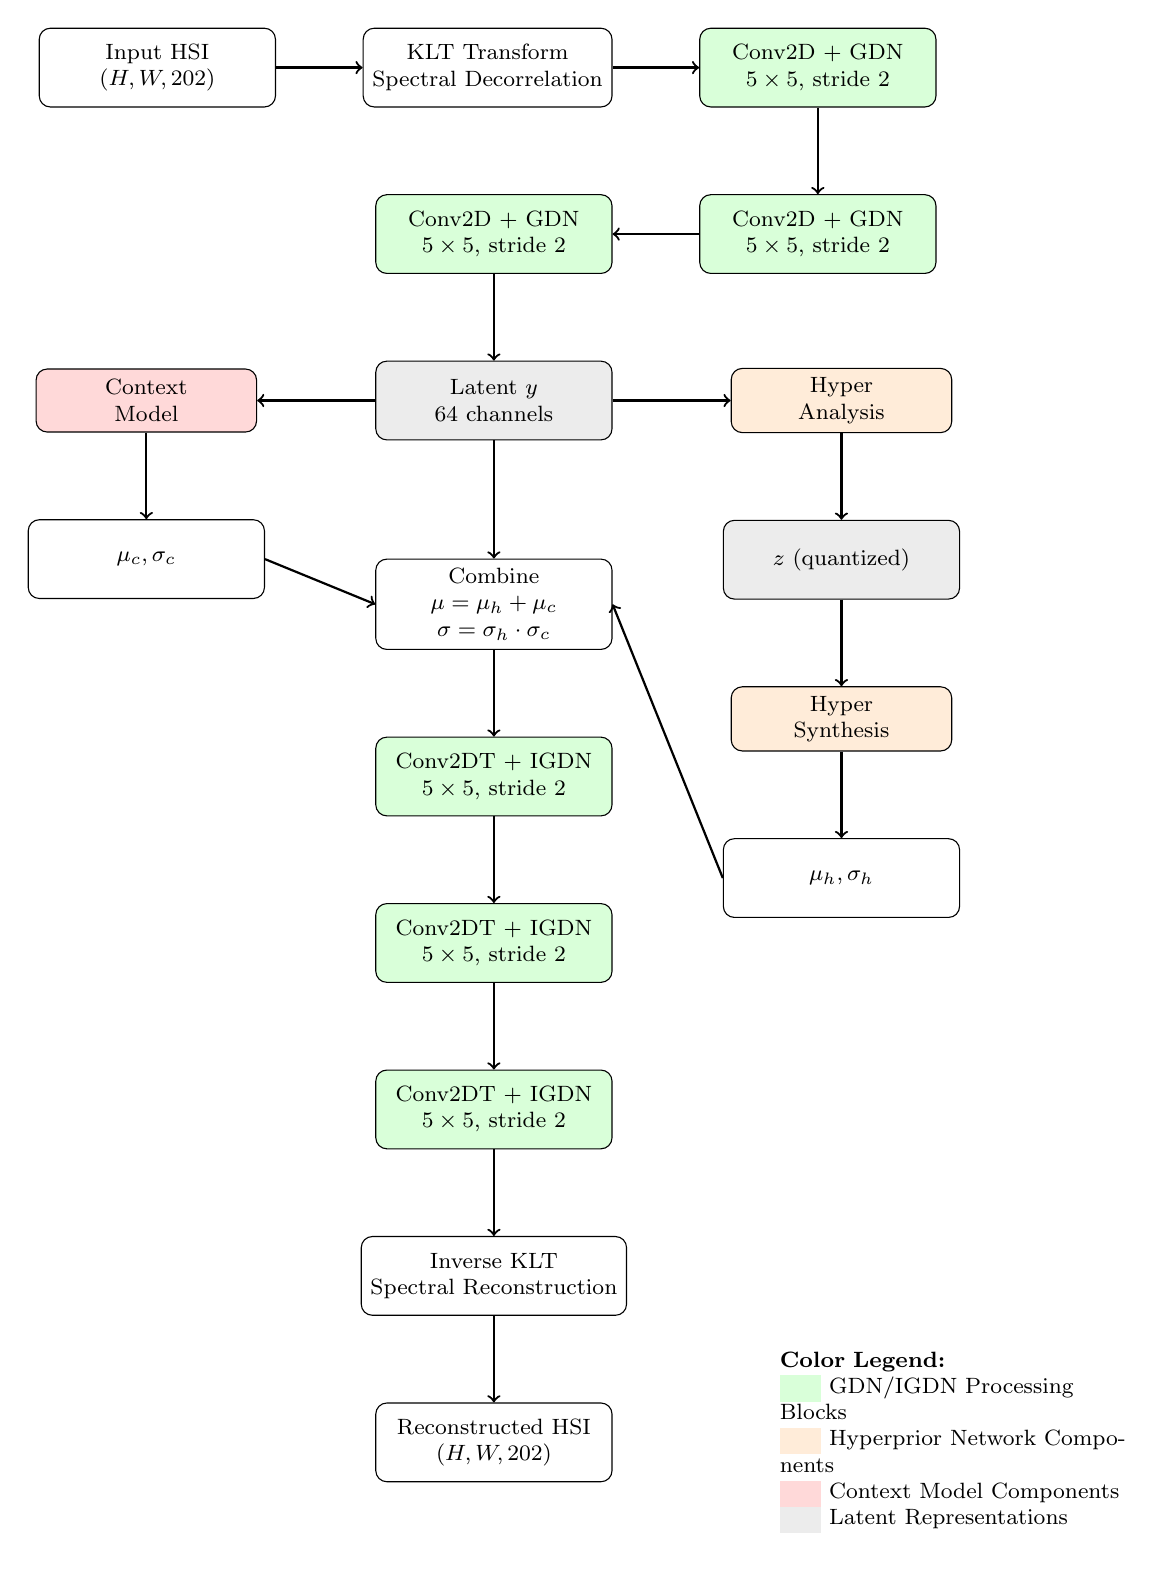
\begin{tikzpicture}[
            block/.style={draw, rounded corners, minimum width=3cm, minimum height=1cm, align=center, font=\footnotesize},
            gdnblock/.style={draw, rounded corners, minimum width=3cm, minimum height=1cm, align=center, fill=green!15, font=\footnotesize},
            hyperblock/.style={draw, rounded corners, minimum width=2.8cm, minimum height=0.8cm, align=center, fill=orange!15, font=\footnotesize},
            contextblock/.style={draw, rounded corners, minimum width=2.8cm, minimum height=0.8cm, align=center, fill=red!15, font=\footnotesize},
            latent/.style={draw, rounded corners, minimum width=3cm, minimum height=1cm, align=center, fill=gray!15, font=\footnotesize},
            arrow/.style={->, thick},
            node distance=1.1cm
        ]

        % Main encoder path
        \node[block] (input) {Input HSI\\$(H,W,202)$};
        \node[block, right=of input] (klt) {KLT Transform\\Spectral Decorrelation};
        \node[gdnblock, right=of klt] (enc1) {Conv2D + GDN\\$5 \times 5$, stride 2};
        \node[gdnblock, below=of enc1] (enc2) {Conv2D + GDN\\$5 \times 5$, stride 2};
        \node[gdnblock, left=of enc2] (enc3) {Conv2D + GDN\\$5 \times 5$, stride 2};
        \node[latent, below=of enc3] (latent) {Latent $y$\\64 channels};

        % Hyperprior branch
        \node[hyperblock, right=1.5cm of latent] (hyperenc) {Hyper\\Analysis};
        \node[latent, below=of hyperenc] (hyperlatent) {$z$ (quantized)};
        \node[hyperblock, below=of hyperlatent] (hyperdec) {Hyper\\Synthesis};
        \node[block, below=of hyperdec] (hyperparams) {$\mu_h, \sigma_h$};

        % Context model
        \node[contextblock, left=1.5cm of latent] (context) {Context\\Model};
        \node[block, below=of context] (contextparams) {$\mu_c, \sigma_c$};

        % Parameter combination
        \node[block, below=1.5cm of latent] (combine) {Combine\\$\mu = \mu_h + \mu_c$\\$\sigma = \sigma_h \cdot \sigma_c$};

        % Decoder path
        \node[gdnblock, below=of combine] (dec1) {Conv2DT + IGDN\\$5 \times 5$, stride 2};
        \node[gdnblock, below=of dec1] (dec2) {Conv2DT + IGDN\\$5 \times 5$, stride 2};
        \node[gdnblock, below=of dec2] (dec3) {Conv2DT + IGDN\\$5 \times 5$, stride 2};
        \node[block, below=of dec3] (iklt) {Inverse KLT\\Spectral Reconstruction};
        \node[block, below=of iklt] (output) {Reconstructed HSI\\$(H,W,202)$};

        % Main path arrows
        \draw[arrow] (input) -- (klt);
        \draw[arrow] (klt) -- (enc1);
        \draw[arrow] (enc1) -- (enc2);
        \draw[arrow] (enc2) -- (enc3);
        \draw[arrow] (enc3) -- (latent);
        \draw[arrow] (latent) -- (combine);
        \draw[arrow] (combine) -- (dec1);
        \draw[arrow] (dec1) -- (dec2);
        \draw[arrow] (dec2) -- (dec3);
        \draw[arrow] (dec3) -- (iklt);
        \draw[arrow] (iklt) -- (output);

        % Hyperprior arrows
        \draw[arrow] (latent.east) -- (hyperenc.west);
        \draw[arrow] (hyperenc) -- (hyperlatent);
        \draw[arrow] (hyperlatent) -- (hyperdec);
        \draw[arrow] (hyperdec) -- (hyperparams);
        \draw[arrow] (hyperparams.west) -- (combine.east);

        % Context arrows
        \draw[arrow] (latent.west) -- (context.east);
        \draw[arrow] (context) -- (contextparams);
        \draw[arrow] (contextparams.east) -- (combine.west);

        % Color legend
        \node[right=2cm of output, text width=4.5cm, align=left, font=\footnotesize] (legend) {
            \textbf{Color Legend:}\\
            \colorbox{green!15}{\phantom{xx}} GDN/IGDN Processing Blocks\\
            \colorbox{orange!15}{\phantom{xx}} Hyperprior Network Components\\
            \colorbox{red!15}{\phantom{xx}} Context Model Components\\
            \colorbox{gray!15}{\phantom{xx}} Latent Representations
        };
    \end{tikzpicture}
    \caption{RCGDNAE architecture with KLT preprocessing, GDN/IGDN layers, hyperprior network, and context model for variable-rate lossy HSI compression.}
    \label{fig:rcgdnae_architecture}
\end{figure}

\subsection{General Divisive Normalisation}
The GDN layer applies a non-linear transformation to the data at its input, which helps to capture complex relationships between the input features.
The GDN transformation's mathematical definition is given by equation \ref{fig:gdnl_equation}:
\begin{align}
    y_i = \frac{x_i}{\left( \beta_i + \sum_{j} \gamma_{ij} |x_j|^{\alpha} \right)^{\frac{1}{\alpha}}}
    \label{fig:gdnl_equation}
\end{align}
where \( y_i \) is the output of the GDN layer, \( x_i \) is the input, \( \beta_i \) and \( \gamma_{ij} \) are learnable parameters, and \( \alpha \) is a hyperparameter that controls the non-linearity of the transformation.
The GDN function is particularly effective for image compression tasks as it has been shown to improve the entropy of the latent representation which, in turn, leads to higher compression ratios.

\subsection{Karhunen-Loève Transform}
The KLT is a linear transformation that decorrelates the input data by projecting it onto a new surface defined by the eigenvectors of the data's covariance matrix~\cite{KLTSrc}.
This transformation is useful as it maximizes the variance along each new axis, allowing for more efficient compression.
The KLT is defined mathematically by equation \ref{fig:klt_equation}:
\begin{align}
    y = W^T (x - \mu)
    \label{fig:klt_equation}
\end{align}
where \( y \) is the transformed data, \( W \) is the matrix of eigenvectors, \( x \) is the input data, and \( \mu \) is the mean of the input data.
To ensure the model has a low computational complexity, the \( W \) matrix used was precomputed from the training dataset and is fixed during training of the rest of the model.

\subsection{Hyperprior network}
The hyperprior network is an additional neural network that models the distribution of the points in the latent space produced by the encoder.
It consists of two parts: a hyperprior analysis network and a hyperprior synthesis network.
The hyperprior analysis network takes the latent representation from the encoder and produces a set of parameters that describe the distribution of the latent space.
The hyperprior synthesis network then uses these parameters to generate a set of mean and standard deviation values that are used to model the distribution of the latent representation for entropy coding.
This approach allows for better compression performance by providing more accurate estimates of the latent representation's distribution for entropy coding.

\subsection{Autoregressive context model}
The autoregressive context model is used to further improve the entropy coding of the latent representation.
It models the dependencies between different elements in the latent space by conditioning the probability of each element on the previous elements.
This is achieved using a series of convolutional layers that process the latent representation in a sequential manner.
The output of the context model is then combined with the output of the hyperprior synthesis network to produce the final mean and standard deviation values used for entropy coding.

\subsection{Variable Encoding Rate}
To enable variable encoding rates, the model incorporates a rate-distortion trade-off mechanism.
During training, a Lagrangian multiplier \( \lambda \) is introduced to balance the trade-off between the bitrate and the distortion of the reconstructed image.
By adjusting \( \lambda \), the model can be trained to prioritize either lower bitrate or higher reconstruction quality, allowing for flexible encoding rates based on application requirements.
The lambda value is incorporated into the loss function as follows:
\begin{align}
    L = D + \lambda R
\end{align}
where \( L \) is the total loss, \( D \) is the distortion (measured by MAE), \( R \) is the estimated bitrate, and \( \lambda \) is the Lagrangian multiplier.
Three versions of the model were trained with different \( \lambda \) values: 0 (pure MAE loss), 0.001, and 0.01.
These different models allow for the evaluation of the trade-off between compression rate and reconstruction quality.

\subsection{Model implementation}
The RCGDNAE model was implemented using the TensorFlow framework.
The model, and all of the non-standard layers are defined in the \mintinline{python}|RCGDNAE.py| file.
The encoder itself was constructed using four GDN layers interleaved with convolutional layers that progressively reduce the spatial dimensions of the input data.
The decoder mirrors this structure using inverse GDN layers and transposed convolutional layers to reconstruct the original data.
The hyperprior network and context model were also implemented using convolutional layers, with the hyperprior analysis network reducing the spatial dimensions of the latent representation and the hyperprior synthesis network increasing them back to match the latent representation's dimensions.
The context model processes the latent representation using masked convolutions to ensure the autoregressive property is maintained.


\section{Training}
The model was trained in three different configurations corresponding to different target bitrates, achieved by varying the Lagrangian multiplier \( \lambda \) in the loss function.
The three configurations are referred to as RCGDNAE-Low, RCGDNAE-Medium, and RCGDNAE-High, corresponding to \( \lambda \) values of 0.01, 0.001, and 0, respectively.
The training procedure for all three configurations was identical, with the only difference being the value of \( \lambda \) used in the loss function.
The training consisted of 100 epochs and a learning rate of 0.0001 for the RCGDNAE-Medium and RCGDNAE-High models, while the RCGDNAE-Low model was trained for 500 epochs with a learning rate of 0.00001.
The curves for the monitored metrics for each model can be seen in Figures \ref{fig:training_metrics_rcgdnae_low}, \ref{fig:training_metrics_rcgdnae_medium}, and \ref{fig:training_metrics_rcgdnae_high}.

%High

\begin{figure}
    \centering
    \begin{subfigure}{0.45\textwidth}
        \centering
        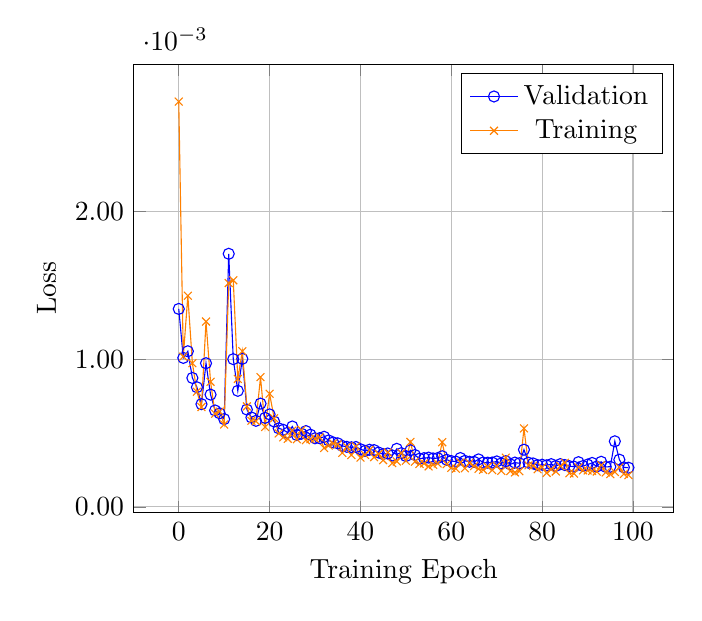
\begin{tikzpicture}
            \begin{axis}[
                    xlabel={Training Epoch},
                    ylabel={Loss},
                    grid=major,
                    y tick label style={
                            /pgf/number format/.cd,
                            fixed,
                            fixed zerofill,
                            precision=2,
                            /tikz/.cd
                        },
                    x tick label style={
                            /pgf/number format/.cd,
                            fixed,
                            fixed zerofill,
                            precision=0,
                            /tikz/.cd
                        }
                ]

                \addplot [color=blue, mark=o] coordinates {
                        (0, 0.0013408823870122433)
                        (1, 0.001009318046271801)
                        (2, 0.0010540480725467205)
                        (3, 0.0008733823779039085)
                        (4, 0.000810313387773931)
                        (5, 0.0006961520412005484)
                        (6, 0.0009731026948429644)
                        (7, 0.0007605649880133569)
                        (8, 0.0006534099229611456)
                        (9, 0.0006342387059703469)
                        (10, 0.0005945888697169721)
                        (11, 0.0017143470467999578)
                        (12, 0.0010007655946537852)
                        (13, 0.0007863874197937548)
                        (14, 0.0010030691046267748)
                        (15, 0.0006594487349502742)
                        (16, 0.0006059634615667164)
                        (17, 0.0005831391317769885)
                        (18, 0.0006997801247052848)
                        (19, 0.0006030757795087993)
                        (20, 0.0006268642609938979)
                        (21, 0.0005781975924037397)
                        (22, 0.0005324852536432445)
                        (23, 0.0005224294727668166)
                        (24, 0.0005027458537369967)
                        (25, 0.0005447134026326239)
                        (26, 0.00048683525528758764)
                        (27, 0.0004960725200362504)
                        (28, 0.0005137157859280705)
                        (29, 0.0004893137374892831)
                        (30, 0.00046476925490424037)
                        (31, 0.0004655819502659142)
                        (32, 0.0004750025400426239)
                        (33, 0.00045044641592539847)
                        (34, 0.000437072740169242)
                        (35, 0.000430926273111254)
                        (36, 0.0004132693575229496)
                        (37, 0.0004068999842274934)
                        (38, 0.00040390563663095236)
                        (39, 0.0004060795472469181)
                        (40, 0.0003910721861757338)
                        (41, 0.0003795684897340834)
                        (42, 0.00038747352664358914)
                        (43, 0.0003849320637527853)
                        (44, 0.0003687598800752312)
                        (45, 0.0003577393072191626)
                        (46, 0.00036204414209350944)
                        (47, 0.0003486601053737104)
                        (48, 0.00039352456224150956)
                        (49, 0.0003640946524683386)
                        (50, 0.00034437928115949035)
                        (51, 0.00038375629810616374)
                        (52, 0.00035152159398421645)
                        (53, 0.0003267855499871075)
                        (54, 0.00033052178332582116)
                        (55, 0.00033405027352273464)
                        (56, 0.0003283489786554128)
                        (57, 0.00033079422428272665)
                        (58, 0.0003432390803936869)
                        (59, 0.00031932684942148626)
                        (60, 0.00031080059125088155)
                        (61, 0.00030723391682840884)
                        (62, 0.0003312032495159656)
                        (63, 0.00031205706181935966)
                        (64, 0.0003059528535231948)
                        (65, 0.0003054123662877828)
                        (66, 0.00032200253917835653)
                        (67, 0.0003008739440701902)
                        (68, 0.000299969658954069)
                        (69, 0.0003006635815836489)
                        (70, 0.00030830182367935777)
                        (71, 0.00029488865402527153)
                        (72, 0.0003095766587648541)
                        (73, 0.0002886927977669984)
                        (74, 0.0003003494639415294)
                        (75, 0.0002957017859444022)
                        (76, 0.00038765821955166757)
                        (77, 0.00029966080910526216)
                        (78, 0.0002947801258414984)
                        (79, 0.00028298338293097913)
                        (80, 0.0002860053791664541)
                        (81, 0.00028175010811537504)
                        (82, 0.0002899030514527112)
                        (83, 0.00027742530801333487)
                        (84, 0.00028997487970627844)
                        (85, 0.0002837185456883162)
                        (86, 0.0002760262577794492)
                        (87, 0.00027320501976646483)
                        (88, 0.00030318618519231677)
                        (89, 0.00027719748322851956)
                        (90, 0.00028704115538857877)
                        (91, 0.0002979531418532133)
                        (92, 0.00027345638955011964)
                        (93, 0.0003056997957173735)
                        (94, 0.0002713636786211282)
                        (95, 0.00027218885952606797)
                        (96, 0.00044449089909903705)
                        (97, 0.0003202533698640764)
                        (98, 0.00026764682843349874)
                        (99, 0.0002658982411958277)
                    };
                \addlegendentry{Validation}

                \addplot [color=orange, mark=x] coordinates {
                        (0, 0.0027451037894934416)
                        (1, 0.0010182932019233704)
                        (2, 0.0014303760835900903)
                        (3, 0.0009735837811604142)
                        (4, 0.0007799045997671783)
                        (5, 0.0006765142315998673)
                        (6, 0.0012555608991533518)
                        (7, 0.000847388815600425)
                        (8, 0.0006313820485956967)
                        (9, 0.000646305619738996)
                        (10, 0.0005581427831202745)
                        (11, 0.0015161809278652072)
                        (12, 0.0015348209999501705)
                        (13, 0.000866939255502075)
                        (14, 0.001054734573699534)
                        (15, 0.0006809369078837335)
                        (16, 0.0005835980409756303)
                        (17, 0.0005804354441352189)
                        (18, 0.0008790509309619665)
                        (19, 0.0005414694314822555)
                        (20, 0.0007665631710551679)
                        (21, 0.0006007516640238464)
                        (22, 0.0004981778329238296)
                        (23, 0.0004712180234491825)
                        (24, 0.0004615687648765743)
                        (25, 0.0005171071970835328)
                        (26, 0.00045869918540120125)
                        (27, 0.0005215738783590496)
                        (28, 0.0004520252696238458)
                        (29, 0.0004588160081766546)
                        (30, 0.0004627207526937127)
                        (31, 0.00047055017785169184)
                        (32, 0.00039909753832034767)
                        (33, 0.00041591149056330323)
                        (34, 0.0004300094733480364)
                        (35, 0.00042367898277007043)
                        (36, 0.00036581215681508183)
                        (37, 0.0004078452766407281)
                        (38, 0.0003511991526465863)
                        (39, 0.0004111361922696233)
                        (40, 0.00033412876655347645)
                        (41, 0.00035221740836277604)
                        (42, 0.0003857071278616786)
                        (43, 0.00033706618705764413)
                        (44, 0.000359486963134259)
                        (45, 0.0003167934773955494)
                        (46, 0.00036896771052852273)
                        (47, 0.0002965634048450738)
                        (48, 0.0003079429152421653)
                        (49, 0.00036564384936355054)
                        (50, 0.0003126290685031563)
                        (51, 0.00044052102020941675)
                        (52, 0.00030652619898319244)
                        (53, 0.00029109278693795204)
                        (54, 0.0002945726446341723)
                        (55, 0.000274281861493364)
                        (56, 0.00028540377388708293)
                        (57, 0.0002942285791505128)
                        (58, 0.0004382233018986881)
                        (59, 0.0002895371872000396)
                        (60, 0.00026436045300215483)
                        (61, 0.0002592174569144845)
                        (62, 0.0003015587280970067)
                        (63, 0.00026225580950267613)
                        (64, 0.0002987754705827683)
                        (65, 0.0002764123782981187)
                        (66, 0.0002582952147349715)
                        (67, 0.0002513206854928285)
                        (68, 0.00027300420333631337)
                        (69, 0.00024914529058150947)
                        (70, 0.00027827126905322075)
                        (71, 0.00024397500965278596)
                        (72, 0.00033376028295606375)
                        (73, 0.0002428865700494498)
                        (74, 0.00023377261823043227)
                        (75, 0.0002418147778371349)
                        (76, 0.0005318278563208878)
                        (77, 0.0002814315666910261)
                        (78, 0.0002789398131426424)
                        (79, 0.0002552447549533099)
                        (80, 0.00026837436598725617)
                        (81, 0.00023020512890070677)
                        (82, 0.00025498910690657794)
                        (83, 0.0002401765959803015)
                        (84, 0.00027662963839247823)
                        (85, 0.00029914834885858)
                        (86, 0.00022795239055994898)
                        (87, 0.00022619767696596682)
                        (88, 0.00026845515822060406)
                        (89, 0.00024806035798974335)
                        (90, 0.00024689221754670143)
                        (91, 0.0002435100032016635)
                        (92, 0.00023948684975039214)
                        (93, 0.00028289289912208915)
                        (94, 0.0002336001198273152)
                        (95, 0.00022197126236278564)
                        (96, 0.00023640358995180577)
                        (97, 0.0002683849597815424)
                        (98, 0.00022375125263351947)
                        (99, 0.00021524477051571012)
                    };
                \addlegendentry{Training}

            \end{axis}
        \end{tikzpicture}
        \caption{Loss over Epochs}
        \label{fig:loss_rcgdnae_high}
    \end{subfigure}
    \hfill
    \begin{subfigure}{0.45\textwidth}
        \centering
        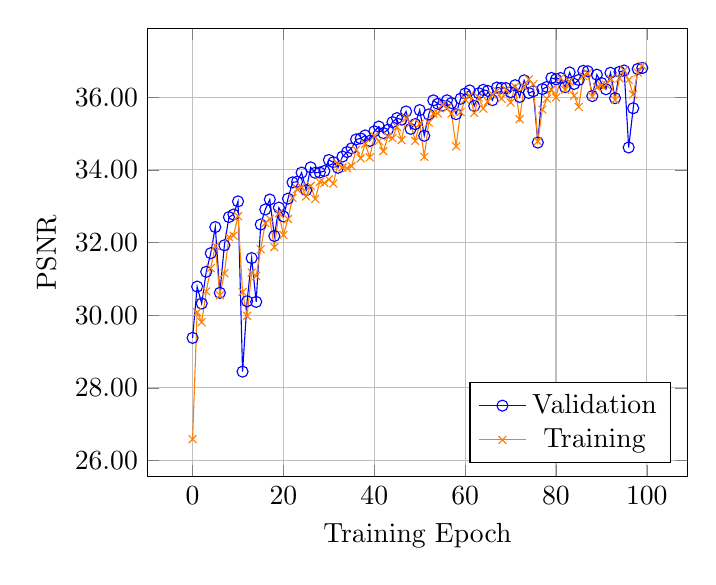
\begin{tikzpicture}
            \begin{axis}[
                    legend pos = south east,
                    xlabel={Training Epoch},
                    ylabel={PSNR},
                    grid=major,
                    y tick label style={
                            /pgf/number format/.cd,
                            fixed,
                            fixed zerofill,
                            precision=2,
                            /tikz/.cd
                        },
                    x tick label style={
                            /pgf/number format/.cd,
                            fixed,
                            fixed zerofill,
                            precision=0,
                            /tikz/.cd
                        }
                ]

                \addplot [color=blue, mark=o] coordinates {
                        (0, 29.378028869628906)
                        (1, 30.78899383544922)
                        (2, 30.324321746826172)
                        (3, 31.196849822998047)
                        (4, 31.708786010742188)
                        (5, 32.42761993408203)
                        (6, 30.618471145629883)
                        (7, 31.926536560058594)
                        (8, 32.702789306640625)
                        (9, 32.772705078125)
                        (10, 33.13385009765625)
                        (11, 28.448942184448242)
                        (12, 30.38679313659668)
                        (13, 31.573747634887695)
                        (14, 30.368989944458008)
                        (15, 32.49789047241211)
                        (16, 32.91170120239258)
                        (17, 33.18570327758789)
                        (18, 32.18272399902344)
                        (19, 32.963294982910156)
                        (20, 32.720523834228516)
                        (21, 33.20968246459961)
                        (22, 33.657596588134766)
                        (23, 33.6766357421875)
                        (24, 33.92611312866211)
                        (25, 33.44185256958008)
                        (26, 34.07108688354492)
                        (27, 33.920711517333984)
                        (28, 33.930137634277344)
                        (29, 33.971214294433594)
                        (30, 34.27383041381836)
                        (31, 34.212310791015625)
                        (32, 34.0590705871582)
                        (33, 34.36754608154297)
                        (34, 34.49312973022461)
                        (35, 34.595237731933594)
                        (36, 34.83879852294922)
                        (37, 34.86773681640625)
                        (38, 34.949275970458984)
                        (39, 34.80120086669922)
                        (40, 35.06227111816406)
                        (41, 35.19329071044922)
                        (42, 35.01583480834961)
                        (43, 35.10799026489258)
                        (44, 35.3153076171875)
                        (45, 35.42652893066406)
                        (46, 35.384761810302734)
                        (47, 35.60940933227539)
                        (48, 35.130287170410156)
                        (49, 35.261009216308594)
                        (50, 35.647850036621094)
                        (51, 34.94188690185547)
                        (52, 35.527000427246094)
                        (53, 35.914730072021484)
                        (54, 35.820762634277344)
                        (55, 35.772029876708984)
                        (56, 35.916866302490234)
                        (57, 35.84132385253906)
                        (58, 35.536624908447266)
                        (59, 35.96004867553711)
                        (60, 36.10319519042969)
                        (61, 36.18790054321289)
                        (62, 35.75959396362305)
                        (63, 36.1109619140625)
                        (64, 36.204647064208984)
                        (65, 36.17427062988281)
                        (66, 35.92027282714844)
                        (67, 36.267860412597656)
                        (68, 36.25808334350586)
                        (69, 36.252113342285156)
                        (70, 36.14115524291992)
                        (71, 36.331729888916016)
                        (72, 36.00931167602539)
                        (73, 36.465965270996094)
                        (74, 36.11819076538086)
                        (75, 36.16587448120117)
                        (76, 34.75260925292969)
                        (77, 36.225284576416016)
                        (78, 36.28321838378906)
                        (79, 36.53165054321289)
                        (80, 36.49433135986328)
                        (81, 36.5288200378418)
                        (82, 36.27973556518555)
                        (83, 36.68297576904297)
                        (84, 36.36736297607422)
                        (85, 36.476749420166016)
                        (86, 36.72718048095703)
                        (87, 36.71512222290039)
                        (88, 36.0335578918457)
                        (89, 36.622047424316406)
                        (90, 36.39165496826172)
                        (91, 36.221290588378906)
                        (92, 36.673728942871094)
                        (93, 35.97635269165039)
                        (94, 36.70039749145508)
                        (95, 36.736717224121094)
                        (96, 34.61801528930664)
                        (97, 35.6983757019043)
                        (98, 36.779048919677734)
                        (99, 36.80583572387695)
                    };
                \addlegendentry{Validation}

                \addplot [color=orange, mark=x] coordinates {
                        (0, 26.589628219604492)
                        (1, 30.079811096191406)
                        (2, 29.80699920654297)
                        (3, 30.656082153320312)
                        (4, 31.299392700195312)
                        (5, 31.906780242919922)
                        (6, 30.549543380737305)
                        (7, 31.15776824951172)
                        (8, 32.154293060302734)
                        (9, 32.19157409667969)
                        (10, 32.72627258300781)
                        (11, 30.642053604125977)
                        (12, 29.984783172607422)
                        (13, 31.174148559570312)
                        (14, 31.081727981567383)
                        (15, 31.81446647644043)
                        (16, 32.53641128540039)
                        (17, 32.65086364746094)
                        (18, 31.874902725219727)
                        (19, 32.80453872680664)
                        (20, 32.21161651611328)
                        (21, 32.65009689331055)
                        (22, 33.22929382324219)
                        (23, 33.469966888427734)
                        (24, 33.526573181152344)
                        (25, 33.26924133300781)
                        (26, 33.56365966796875)
                        (27, 33.20154571533203)
                        (28, 33.66963195800781)
                        (29, 33.63932800292969)
                        (30, 33.73915100097656)
                        (31, 33.62535095214844)
                        (32, 34.171138763427734)
                        (33, 34.06679153442383)
                        (34, 34.05096435546875)
                        (35, 34.10368347167969)
                        (36, 34.5552864074707)
                        (37, 34.31882095336914)
                        (38, 34.71878433227539)
                        (39, 34.34765625)
                        (40, 34.931373596191406)
                        (41, 34.7972297668457)
                        (42, 34.51698303222656)
                        (43, 34.921287536621094)
                        (44, 34.876319885253906)
                        (45, 35.187461853027344)
                        (46, 34.818809509277344)
                        (47, 35.43168640136719)
                        (48, 35.29228210449219)
                        (49, 34.79823684692383)
                        (50, 35.27495193481445)
                        (51, 34.359195709228516)
                        (52, 35.30215072631836)
                        (53, 35.550331115722656)
                        (54, 35.551971435546875)
                        (55, 35.79875946044922)
                        (56, 35.69862747192383)
                        (57, 35.549381256103516)
                        (58, 34.651275634765625)
                        (59, 35.594234466552734)
                        (60, 35.93716812133789)
                        (61, 36.0410041809082)
                        (62, 35.56998825073242)
                        (63, 35.99024200439453)
                        (64, 35.68718719482422)
                        (65, 35.884185791015625)
                        (66, 36.078895568847656)
                        (67, 36.17523193359375)
                        (68, 35.960697174072266)
                        (69, 36.20563507080078)
                        (70, 35.856239318847656)
                        (71, 36.29010772705078)
                        (72, 35.39841079711914)
                        (73, 36.287452697753906)
                        (74, 36.49089813232422)
                        (75, 36.35565948486328)
                        (76, 34.786888122558594)
                        (77, 35.662567138671875)
                        (78, 35.960811614990234)
                        (79, 36.211692810058594)
                        (80, 35.995811462402344)
                        (81, 36.535072326660156)
                        (82, 36.20524978637695)
                        (83, 36.4343376159668)
                        (84, 36.04512023925781)
                        (85, 35.736595153808594)
                        (86, 36.583309173583984)
                        (87, 36.65877151489258)
                        (88, 36.021446228027344)
                        (89, 36.27508544921875)
                        (90, 36.329010009765625)
                        (91, 36.34721755981445)
                        (92, 36.513916015625)
                        (93, 35.927734375)
                        (94, 36.521976470947266)
                        (95, 36.73811721801758)
                        (96, 36.47840881347656)
                        (97, 36.07741165161133)
                        (98, 36.68027877807617)
                        (99, 36.87196731567383)
                    };
                \addlegendentry{Training}

            \end{axis}
        \end{tikzpicture}
        \caption{PSNR over Epochs}
        \label{fig:psnr_rcgdnae_high}
    \end{subfigure}

    \begin{subfigure}{0.45\textwidth}
        \centering
        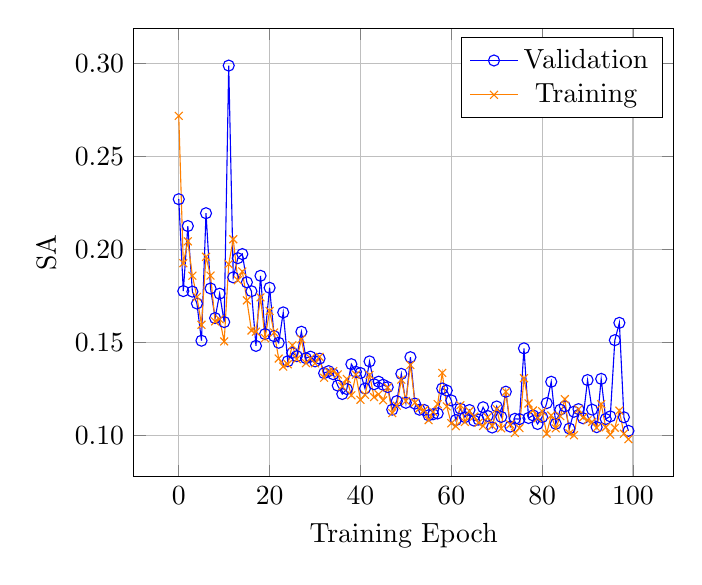
\begin{tikzpicture}
            \begin{axis}[
                    xlabel={Training Epoch},
                    ylabel={SA},
                    grid=major,
                    y tick label style={
                            /pgf/number format/.cd,
                            fixed,
                            fixed zerofill,
                            precision=2,
                            /tikz/.cd
                        },
                    x tick label style={
                            /pgf/number format/.cd,
                            fixed,
                            fixed zerofill,
                            precision=0,
                            /tikz/.cd
                        }
                ]

                \addplot [color=blue, mark=o] coordinates {
                        (0, 0.22714796662330627)
                        (1, 0.17771822214126587)
                        (2, 0.21270498633384705)
                        (3, 0.1774456650018692)
                        (4, 0.17105232179164886)
                        (5, 0.1510455310344696)
                        (6, 0.21960216760635376)
                        (7, 0.17914213240146637)
                        (8, 0.16321048140525818)
                        (9, 0.17633724212646484)
                        (10, 0.16107754409313202)
                        (11, 0.2989906668663025)
                        (12, 0.18511272966861725)
                        (13, 0.19542177021503448)
                        (14, 0.19762317836284637)
                        (15, 0.18244263529777527)
                        (16, 0.17766106128692627)
                        (17, 0.14825144410133362)
                        (18, 0.18595144152641296)
                        (19, 0.15460316836833954)
                        (20, 0.17949917912483215)
                        (21, 0.1534731239080429)
                        (22, 0.14994357526302338)
                        (23, 0.16625969111919403)
                        (24, 0.13998879492282867)
                        (25, 0.1444920301437378)
                        (26, 0.1427365243434906)
                        (27, 0.15585441887378693)
                        (28, 0.141643688082695)
                        (29, 0.14247150719165802)
                        (30, 0.1399565190076828)
                        (31, 0.14139452576637268)
                        (32, 0.1335829198360443)
                        (33, 0.1346733570098877)
                        (34, 0.1330249160528183)
                        (35, 0.12689857184886932)
                        (36, 0.1223929226398468)
                        (37, 0.12505562603473663)
                        (38, 0.13843543827533722)
                        (39, 0.13432233035564423)
                        (40, 0.13365882635116577)
                        (41, 0.1253392994403839)
                        (42, 0.13992074131965637)
                        (43, 0.12764635682106018)
                        (44, 0.12900005280971527)
                        (45, 0.1273435354232788)
                        (46, 0.12609855830669403)
                        (47, 0.11399085074663162)
                        (48, 0.11855582892894745)
                        (49, 0.13321198523044586)
                        (50, 0.11766032129526138)
                        (51, 0.14217811822891235)
                        (52, 0.11723543703556061)
                        (53, 0.11395039409399033)
                        (54, 0.1138201355934143)
                        (55, 0.11093524843454361)
                        (56, 0.1114877387881279)
                        (57, 0.1119205504655838)
                        (58, 0.12534809112548828)
                        (59, 0.12425797432661057)
                        (60, 0.11893731355667114)
                        (61, 0.10834798961877823)
                        (62, 0.11452151834964752)
                        (63, 0.10992198437452316)
                        (64, 0.11375683546066284)
                        (65, 0.10807710140943527)
                        (66, 0.10862193256616592)
                        (67, 0.11525704711675644)
                        (68, 0.11058790236711502)
                        (69, 0.1043691635131836)
                        (70, 0.11567066609859467)
                        (71, 0.11008409410715103)
                        (72, 0.12363408505916595)
                        (73, 0.10486166924238205)
                        (74, 0.10903669893741608)
                        (75, 0.10886526107788086)
                        (76, 0.1469382643699646)
                        (77, 0.10948602855205536)
                        (78, 0.11088240146636963)
                        (79, 0.1062704399228096)
                        (80, 0.10998951643705368)
                        (81, 0.11747285723686218)
                        (82, 0.12896308302879333)
                        (83, 0.10634896904230118)
                        (84, 0.11395391821861267)
                        (85, 0.11574959754943848)
                        (86, 0.10380823910236359)
                        (87, 0.11284689605236053)
                        (88, 0.11424151062965393)
                        (89, 0.10935292392969131)
                        (90, 0.12988553941249847)
                        (91, 0.11398348957300186)
                        (92, 0.1045665442943573)
                        (93, 0.13052669167518616)
                        (94, 0.10893968492746353)
                        (95, 0.11035521328449249)
                        (96, 0.1513383388519287)
                        (97, 0.16064637899398804)
                        (98, 0.1098756492137909)
                        (99, 0.10257425904273987)
                    };
                \addlegendentry{Validation}

                \addplot [color=orange, mark=x] coordinates {
                        (0, 0.27197447419166565)
                        (1, 0.19272087514400482)
                        (2, 0.2044689804315567)
                        (3, 0.18599779903888702)
                        (4, 0.1746109127998352)
                        (5, 0.15960930287837982)
                        (6, 0.19617201387882233)
                        (7, 0.18606163561344147)
                        (8, 0.16140632331371307)
                        (9, 0.162570521235466)
                        (10, 0.1506664901971817)
                        (11, 0.19216382503509521)
                        (12, 0.20561015605926514)
                        (13, 0.18356719613075256)
                        (14, 0.18827548623085022)
                        (15, 0.17273342609405518)
                        (16, 0.15648986399173737)
                        (17, 0.1558687537908554)
                        (18, 0.1743423491716385)
                        (19, 0.15243779122829437)
                        (20, 0.167075052857399)
                        (21, 0.1554412990808487)
                        (22, 0.1414482146501541)
                        (23, 0.13715915381908417)
                        (24, 0.13837885856628418)
                        (25, 0.1486137956380844)
                        (26, 0.14116081595420837)
                        (27, 0.15185107290744781)
                        (28, 0.13898470997810364)
                        (29, 0.14157931506633759)
                        (30, 0.13888034224510193)
                        (31, 0.14236848056316376)
                        (32, 0.131133034825325)
                        (33, 0.13441050052642822)
                        (34, 0.1346583217382431)
                        (35, 0.13289885222911835)
                        (36, 0.12645071744918823)
                        (37, 0.13049572706222534)
                        (38, 0.12166999280452728)
                        (39, 0.13278210163116455)
                        (40, 0.11926281452178955)
                        (41, 0.12191107869148254)
                        (42, 0.13265493512153625)
                        (43, 0.12073832005262375)
                        (44, 0.12219999730587006)
                        (45, 0.11897870153188705)
                        (46, 0.12590357661247253)
                        (47, 0.11209084093570709)
                        (48, 0.11610748618841171)
                        (49, 0.13011714816093445)
                        (50, 0.11863992363214493)
                        (51, 0.13799719512462616)
                        (52, 0.11768375337123871)
                        (53, 0.11472992599010468)
                        (54, 0.11367166042327881)
                        (55, 0.10832834243774414)
                        (56, 0.11275174468755722)
                        (57, 0.11695132404565811)
                        (58, 0.1337379664182663)
                        (59, 0.11571779102087021)
                        (60, 0.10665985196828842)
                        (61, 0.10510341078042984)
                        (62, 0.1163315400481224)
                        (63, 0.10734300315380096)
                        (64, 0.11322873085737228)
                        (65, 0.11024274677038193)
                        (66, 0.10685952752828598)
                        (67, 0.10518142580986023)
                        (68, 0.10987731069326401)
                        (69, 0.10528033971786499)
                        (70, 0.1142275407910347)
                        (71, 0.10392004251480103)
                        (72, 0.12359894812107086)
                        (73, 0.10602744668722153)
                        (74, 0.10140155255794525)
                        (75, 0.10408155620098114)
                        (76, 0.13086889684200287)
                        (77, 0.11729639768600464)
                        (78, 0.11353161931037903)
                        (79, 0.10932967811822891)
                        (80, 0.11308657377958298)
                        (81, 0.10105155408382416)
                        (82, 0.11083369702100754)
                        (83, 0.10392645001411438)
                        (84, 0.11047853529453278)
                        (85, 0.119613878428936)
                        (86, 0.1011972427368164)
                        (87, 0.10020812600851059)
                        (88, 0.11410467326641083)
                        (89, 0.1097811833024025)
                        (90, 0.1082320362329483)
                        (91, 0.10737770795822144)
                        (92, 0.10420436412096024)
                        (93, 0.11688517779111862)
                        (94, 0.10450650006532669)
                        (95, 0.10056072473526001)
                        (96, 0.10419680923223495)
                        (97, 0.11346220225095749)
                        (98, 0.10103724151849747)
                        (99, 0.0980864092707634)
                    };
                \addlegendentry{Training}

            \end{axis}
        \end{tikzpicture}
        \caption{SA over Epochs}
        \label{fig:sa_rcgdnae_high}
    \end{subfigure}
    \hfill
    \begin{subfigure}{0.45\textwidth}
        \centering
        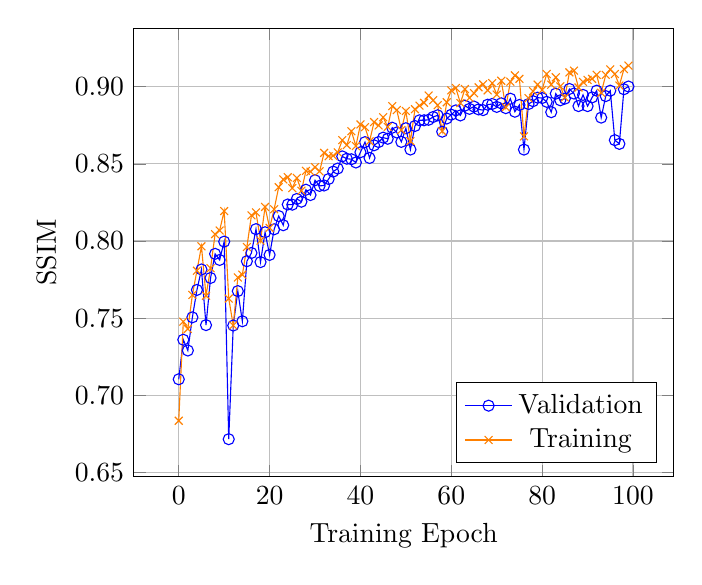
\begin{tikzpicture}
            \begin{axis}[
                    legend pos = south east,
                    xlabel={Training Epoch},
                    ylabel={SSIM},
                    grid=major,
                    y tick label style={
                            /pgf/number format/.cd,
                            fixed,
                            fixed zerofill,
                            precision=2,
                            /tikz/.cd
                        },
                    x tick label style={
                            /pgf/number format/.cd,
                            fixed,
                            fixed zerofill,
                            precision=0,
                            /tikz/.cd
                        }
                ]

                \addplot [color=blue, mark=o] coordinates {
                        (0, 0.7103922367095947)
                        (1, 0.7360063791275024)
                        (2, 0.7290323376655579)
                        (3, 0.7505185604095459)
                        (4, 0.7682731747627258)
                        (5, 0.7815388441085815)
                        (6, 0.7454913258552551)
                        (7, 0.7760335206985474)
                        (8, 0.7916572093963623)
                        (9, 0.7877180576324463)
                        (10, 0.7995860576629639)
                        (11, 0.671556293964386)
                        (12, 0.7452138662338257)
                        (13, 0.7675239443778992)
                        (14, 0.7479687333106995)
                        (15, 0.7868955135345459)
                        (16, 0.792232871055603)
                        (17, 0.8076702356338501)
                        (18, 0.7863200902938843)
                        (19, 0.8056449890136719)
                        (20, 0.790969967842102)
                        (21, 0.8075624108314514)
                        (22, 0.8161698579788208)
                        (23, 0.8102155923843384)
                        (24, 0.8236424326896667)
                        (25, 0.8235230445861816)
                        (26, 0.8272371888160706)
                        (27, 0.8254581093788147)
                        (28, 0.8332161903381348)
                        (29, 0.829777181148529)
                        (30, 0.8393595814704895)
                        (31, 0.8357012271881104)
                        (32, 0.8359680771827698)
                        (33, 0.8401686549186707)
                        (34, 0.8449498414993286)
                        (35, 0.8469417095184326)
                        (36, 0.8548045754432678)
                        (37, 0.8533109426498413)
                        (38, 0.8529751896858215)
                        (39, 0.8508666753768921)
                        (40, 0.8575170636177063)
                        (41, 0.8640537858009338)
                        (42, 0.8537930846214294)
                        (43, 0.8620139360427856)
                        (44, 0.8641129732131958)
                        (45, 0.8669685125350952)
                        (46, 0.8662330508232117)
                        (47, 0.8734036684036255)
                        (48, 0.8703221678733826)
                        (49, 0.8642212748527527)
                        (50, 0.8730519413948059)
                        (51, 0.8592520356178284)
                        (52, 0.874525249004364)
                        (53, 0.8782120943069458)
                        (54, 0.878210186958313)
                        (55, 0.8785392045974731)
                        (56, 0.8803537487983704)
                        (57, 0.8814460039138794)
                        (58, 0.8708279728889465)
                        (59, 0.879372239112854)
                        (60, 0.8818495869636536)
                        (61, 0.8846313953399658)
                        (62, 0.8813631534576416)
                        (63, 0.8877162933349609)
                        (64, 0.885617733001709)
                        (65, 0.887108325958252)
                        (66, 0.8852513432502747)
                        (67, 0.8848059177398682)
                        (68, 0.8883227705955505)
                        (69, 0.8887888193130493)
                        (70, 0.8868836164474487)
                        (71, 0.8891799449920654)
                        (72, 0.8860827088356018)
                        (73, 0.8922098875045776)
                        (74, 0.8837701082229614)
                        (75, 0.8881476521492004)
                        (76, 0.8592227697372437)
                        (77, 0.8887444734573364)
                        (78, 0.8905858397483826)
                        (79, 0.892874002456665)
                        (80, 0.8926175236701965)
                        (81, 0.8901781439781189)
                        (82, 0.883472740650177)
                        (83, 0.8954870104789734)
                        (84, 0.8911674618721008)
                        (85, 0.8922232985496521)
                        (86, 0.8985164761543274)
                        (87, 0.8955458998680115)
                        (88, 0.8874344229698181)
                        (89, 0.8946700692176819)
                        (90, 0.8874056935310364)
                        (91, 0.8930448889732361)
                        (92, 0.8974036574363708)
                        (93, 0.879951000213623)
                        (94, 0.8938919901847839)
                        (95, 0.897400438785553)
                        (96, 0.8653454780578613)
                        (97, 0.8629267811775208)
                        (98, 0.8983269333839417)
                        (99, 0.9000927209854126)
                    };
                \addlegendentry{Validation}

                \addplot [color=orange, mark=x] coordinates {
                        (0, 0.6835008263587952)
                        (1, 0.747717559337616)
                        (2, 0.7430184483528137)
                        (3, 0.765047550201416)
                        (4, 0.7807421684265137)
                        (5, 0.7965561151504517)
                        (6, 0.7645292282104492)
                        (7, 0.7823230624198914)
                        (8, 0.8044071793556213)
                        (9, 0.806806206703186)
                        (10, 0.8193720579147339)
                        (11, 0.7627218961715698)
                        (12, 0.7452832460403442)
                        (13, 0.7763482928276062)
                        (14, 0.7781876921653748)
                        (15, 0.7960618138313293)
                        (16, 0.8165764808654785)
                        (17, 0.8185521364212036)
                        (18, 0.8002293109893799)
                        (19, 0.8220484852790833)
                        (20, 0.8085235357284546)
                        (21, 0.8205883502960205)
                        (22, 0.8348716497421265)
                        (23, 0.8398793935775757)
                        (24, 0.8413111567497253)
                        (25, 0.834251880645752)
                        (26, 0.8408387303352356)
                        (27, 0.8325892686843872)
                        (28, 0.8454398512840271)
                        (29, 0.8449075222015381)
                        (30, 0.8478451371192932)
                        (31, 0.8450945615768433)
                        (32, 0.8570961356163025)
                        (33, 0.8549013137817383)
                        (34, 0.8552387356758118)
                        (35, 0.8574394583702087)
                        (36, 0.8653287291526794)
                        (37, 0.8621516823768616)
                        (38, 0.8711153268814087)
                        (39, 0.8615330457687378)
                        (40, 0.8755251169204712)
                        (41, 0.8737632036209106)
                        (42, 0.8646070957183838)
                        (43, 0.877069890499115)
                        (44, 0.8748843669891357)
                        (45, 0.880207896232605)
                        (46, 0.8739454746246338)
                        (47, 0.8873692750930786)
                        (48, 0.8848802447319031)
                        (49, 0.8718775510787964)
                        (50, 0.8842349052429199)
                        (51, 0.8646948933601379)
                        (52, 0.8854020833969116)
                        (53, 0.8877408504486084)
                        (54, 0.8895301222801208)
                        (55, 0.8942532539367676)
                        (56, 0.8912337422370911)
                        (57, 0.8879788517951965)
                        (58, 0.8711445927619934)
                        (59, 0.8899162411689758)
                        (60, 0.8975831270217896)
                        (61, 0.8991411328315735)
                        (62, 0.8893733620643616)
                        (63, 0.8984590768814087)
                        (64, 0.8927299976348877)
                        (65, 0.8957535624504089)
                        (66, 0.8996016979217529)
                        (67, 0.9015197157859802)
                        (68, 0.8976198434829712)
                        (69, 0.9022908210754395)
                        (70, 0.8948807716369629)
                        (71, 0.903812825679779)
                        (72, 0.8866856694221497)
                        (73, 0.9032145142555237)
                        (74, 0.9072911143302917)
                        (75, 0.9050772786140442)
                        (76, 0.8677529692649841)
                        (77, 0.892582356929779)
                        (78, 0.8970656991004944)
                        (79, 0.9013493657112122)
                        (80, 0.8978695273399353)
                        (81, 0.9082170724868774)
                        (82, 0.9012885093688965)
                        (83, 0.9060953855514526)
                        (84, 0.9001868963241577)
                        (85, 0.892974853515625)
                        (86, 0.9092544913291931)
                        (87, 0.910390317440033)
                        (88, 0.899453341960907)
                        (89, 0.9030981063842773)
                        (90, 0.9043974876403809)
                        (91, 0.905067503452301)
                        (92, 0.9076921343803406)
                        (93, 0.8960296511650085)
                        (94, 0.9076378345489502)
                        (95, 0.9111936688423157)
                        (96, 0.9082315564155579)
                        (97, 0.900783896446228)
                        (98, 0.911365807056427)
                        (99, 0.9136636257171631)
                    };
                \addlegendentry{Training}

            \end{axis}
        \end{tikzpicture}
        \caption{SSIM over Epochs}
        \label{fig:ssim_rcgdnae_high}
    \end{subfigure}
    \caption{Training and Validation Metrics over Epochs for RCGDNAE high bitrate model}
    \label{fig:training_metrics_rcgdnae_high}
\end{figure}

%Mid
\begin{figure}
    \centering
    \begin{subfigure}{0.45\textwidth}
        \centering
        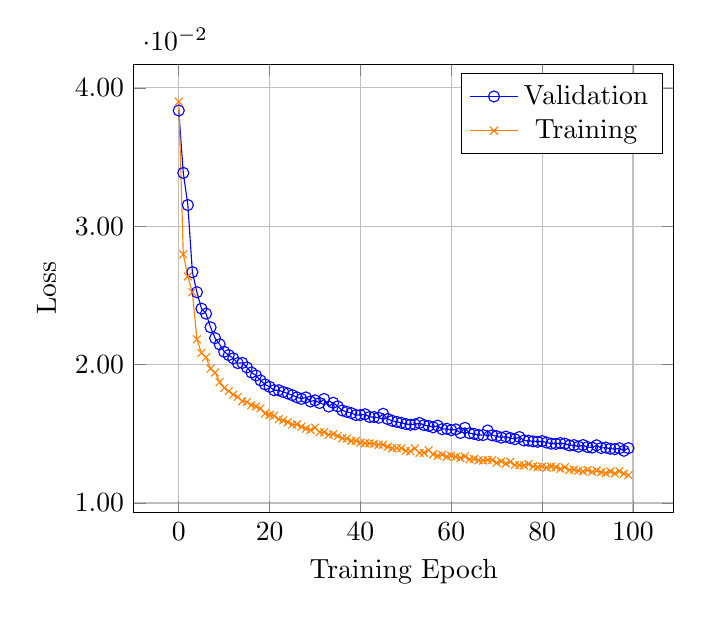
\begin{tikzpicture}
            \begin{axis}[
                    xlabel={Training Epoch},
                    ylabel={Loss},
                    grid=major,
                    y tick label style={
                            /pgf/number format/.cd,
                            fixed,
                            fixed zerofill,
                            precision=2,
                            /tikz/.cd
                        },
                    x tick label style={
                            /pgf/number format/.cd,
                            fixed,
                            fixed zerofill,
                            precision=0,
                            /tikz/.cd
                        }
                ]

                \addplot [color=blue, mark=o] coordinates {
                        (0, 0.038364920765161514)
                        (1, 0.03386060521006584)
                        (2, 0.03153572976589203)
                        (3, 0.026685023680329323)
                        (4, 0.025233855471014977)
                        (5, 0.024048738181591034)
                        (6, 0.02368670143187046)
                        (7, 0.022698218002915382)
                        (8, 0.02191130444407463)
                        (9, 0.02146906964480877)
                        (10, 0.020931778475642204)
                        (11, 0.020689766854047775)
                        (12, 0.020456762984395027)
                        (13, 0.020108701661229134)
                        (14, 0.020125120878219604)
                        (15, 0.019800161942839622)
                        (16, 0.019432825967669487)
                        (17, 0.01921846903860569)
                        (18, 0.01886269450187683)
                        (19, 0.018573341891169548)
                        (20, 0.01839423179626465)
                        (21, 0.018152408301830292)
                        (22, 0.018150335177779198)
                        (23, 0.018024368211627007)
                        (24, 0.017917485907673836)
                        (25, 0.017789926379919052)
                        (26, 0.017639361321926117)
                        (27, 0.017522845417261124)
                        (28, 0.01763257570564747)
                        (29, 0.017338600009679794)
                        (30, 0.017421400174498558)
                        (31, 0.017228037118911743)
                        (32, 0.017516380175948143)
                        (33, 0.016974009573459625)
                        (34, 0.017243970185518265)
                        (35, 0.016985753551125526)
                        (36, 0.016691161319613457)
                        (37, 0.016590720042586327)
                        (38, 0.01649545691907406)
                        (39, 0.016357433050870895)
                        (40, 0.016354765743017197)
                        (41, 0.016418004408478737)
                        (42, 0.016216976568102837)
                        (43, 0.016215024515986443)
                        (44, 0.016161277890205383)
                        (45, 0.016444765031337738)
                        (46, 0.016070419922471046)
                        (47, 0.01594085991382599)
                        (48, 0.015863994136452675)
                        (49, 0.015796927735209465)
                        (50, 0.01570756919682026)
                        (51, 0.015653958544135094)
                        (52, 0.015682796016335487)
                        (53, 0.01578167825937271)
                        (54, 0.01563127525150776)
                        (55, 0.015571090392768383)
                        (56, 0.01547246240079403)
                        (57, 0.015593190677464008)
                        (58, 0.015337860211730003)
                        (59, 0.015369436703622341)
                        (60, 0.01526196300983429)
                        (61, 0.01532110758125782)
                        (62, 0.015063461847603321)
                        (63, 0.01543134544044733)
                        (64, 0.015045695006847382)
                        (65, 0.01499385666102171)
                        (66, 0.014915081672370434)
                        (67, 0.014909138903021812)
                        (68, 0.015240744687616825)
                        (69, 0.014892343431711197)
                        (70, 0.014827797189354897)
                        (71, 0.014724619686603546)
                        (72, 0.014804092235863209)
                        (73, 0.014692341908812523)
                        (74, 0.014612888917326927)
                        (75, 0.014768091961741447)
                        (76, 0.014517765492200851)
                        (77, 0.01450256910175085)
                        (78, 0.014453350566327572)
                        (79, 0.014420637860894203)
                        (80, 0.01447448879480362)
                        (81, 0.01436922512948513)
                        (82, 0.014289251528680325)
                        (83, 0.01427325326949358)
                        (84, 0.014333432540297508)
                        (85, 0.01429140567779541)
                        (86, 0.014161698520183563)
                        (87, 0.014185567386448383)
                        (88, 0.014068122953176498)
                        (89, 0.014191274531185627)
                        (90, 0.014045427553355694)
                        (91, 0.014004230499267578)
                        (92, 0.014169992879033089)
                        (93, 0.013973962515592575)
                        (94, 0.014003810472786427)
                        (95, 0.013925326988101006)
                        (96, 0.013891368173062801)
                        (97, 0.013959798030555248)
                        (98, 0.013774609193205833)
                        (99, 0.013965383172035217)
                    };
                \addlegendentry{Validation}

                \addplot [color=orange, mark=x] coordinates {
                        (0, 0.03901303559541702)
                        (1, 0.027969298884272575)
                        (2, 0.026375358924269676)
                        (3, 0.025225933641195297)
                        (4, 0.021824991330504417)
                        (5, 0.02084808051586151)
                        (6, 0.02052908204495907)
                        (7, 0.019709380343556404)
                        (8, 0.019435733556747437)
                        (9, 0.018722308799624443)
                        (10, 0.01832157000899315)
                        (11, 0.018086465075612068)
                        (12, 0.01783207431435585)
                        (13, 0.017668122425675392)
                        (14, 0.017359238117933273)
                        (15, 0.017296744510531425)
                        (16, 0.017062973231077194)
                        (17, 0.016977015882730484)
                        (18, 0.016840757802128792)
                        (19, 0.016466375440359116)
                        (20, 0.016370082274079323)
                        (21, 0.01630675420165062)
                        (22, 0.01605956070125103)
                        (23, 0.015973346307873726)
                        (24, 0.01583888567984104)
                        (25, 0.015670934692025185)
                        (26, 0.015683457255363464)
                        (27, 0.015517542138695717)
                        (28, 0.01537283230572939)
                        (29, 0.015279782935976982)
                        (30, 0.015446397475898266)
                        (31, 0.015112929977476597)
                        (32, 0.015116773545742035)
                        (33, 0.014929989352822304)
                        (34, 0.014978778548538685)
                        (35, 0.014835488982498646)
                        (36, 0.014678847044706345)
                        (37, 0.01466468907892704)
                        (38, 0.014490736648440361)
                        (39, 0.014494694769382477)
                        (40, 0.014361510053277016)
                        (41, 0.014320684596896172)
                        (42, 0.014309617690742016)
                        (43, 0.014276365749537945)
                        (44, 0.014206337742507458)
                        (45, 0.014206770807504654)
                        (46, 0.014069121330976486)
                        (47, 0.013957522809505463)
                        (48, 0.013969813473522663)
                        (49, 0.013959919102489948)
                        (50, 0.013770606368780136)
                        (51, 0.013733616098761559)
                        (52, 0.013943235389888287)
                        (53, 0.013619656674563885)
                        (54, 0.013627861626446247)
                        (55, 0.013810436241328716)
                        (56, 0.013514096848666668)
                        (57, 0.013418280519545078)
                        (58, 0.013496631756424904)
                        (59, 0.013342877849936485)
                        (60, 0.013422917574644089)
                        (61, 0.013334359973669052)
                        (62, 0.013258795253932476)
                        (63, 0.013367241248488426)
                        (64, 0.013155757449567318)
                        (65, 0.01318324077874422)
                        (66, 0.013086766935884953)
                        (67, 0.013067658990621567)
                        (68, 0.013112189248204231)
                        (69, 0.013111474923789501)
                        (70, 0.012911016121506691)
                        (71, 0.013012368232011795)
                        (72, 0.012853367254137993)
                        (73, 0.012974259443581104)
                        (74, 0.012751703150570393)
                        (75, 0.012735383585095406)
                        (76, 0.012722623534500599)
                        (77, 0.012807263061404228)
                        (78, 0.012642459943890572)
                        (79, 0.01259327307343483)
                        (80, 0.0126344608142972)
                        (81, 0.01256270706653595)
                        (82, 0.012622427195310593)
                        (83, 0.012586738914251328)
                        (84, 0.012469788081943989)
                        (85, 0.012585497461259365)
                        (86, 0.012383305467665195)
                        (87, 0.01241325680166483)
                        (88, 0.01233689021319151)
                        (89, 0.012288573198020458)
                        (90, 0.012385665439069271)
                        (91, 0.012263587675988674)
                        (92, 0.012342607602477074)
                        (93, 0.012218519113957882)
                        (94, 0.012160824611783028)
                        (95, 0.012280415743589401)
                        (96, 0.012140680104494095)
                        (97, 0.012294125743210316)
                        (98, 0.012112884782254696)
                        (99, 0.012012582272291183)
                    };
                \addlegendentry{Training}

            \end{axis}
        \end{tikzpicture}
        \caption{Loss over Epochs}
        \label{fig:loss_mid_rcgdnae}
    \end{subfigure}
    \hfill
    \begin{subfigure}{0.45\textwidth}
        \centering
        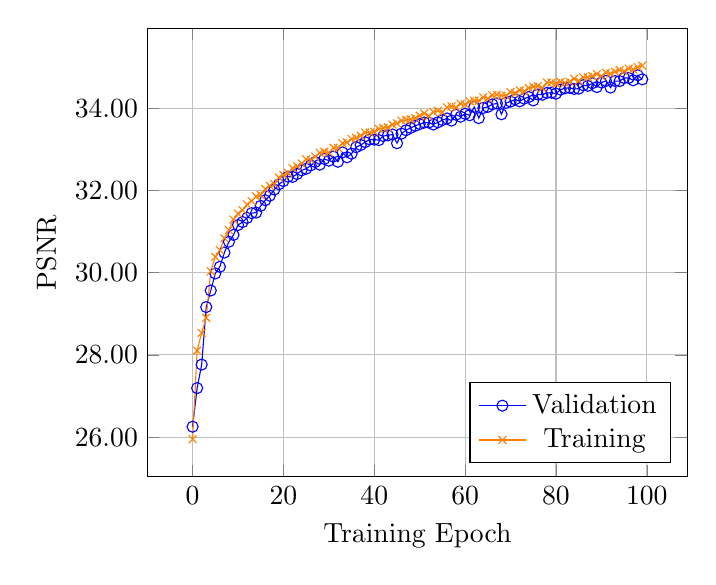
\begin{tikzpicture}
            \begin{axis}[
                    legend pos = south east,
                    xlabel={Training Epoch},
                    ylabel={PSNR},
                    grid=major,
                    y tick label style={
                            /pgf/number format/.cd,
                            fixed,
                            fixed zerofill,
                            precision=2,
                            /tikz/.cd
                        },
                    x tick label style={
                            /pgf/number format/.cd,
                            fixed,
                            fixed zerofill,
                            precision=0,
                            /tikz/.cd
                        }
                ]

                \addplot [color=blue, mark=o] coordinates {
                        (0, 26.254270553588867)
                        (1, 27.193098068237305)
                        (2, 27.76522445678711)
                        (3, 29.163103103637695)
                        (4, 29.566659927368164)
                        (5, 29.981199264526367)
                        (6, 30.14321517944336)
                        (7, 30.489171981811523)
                        (8, 30.752981185913086)
                        (9, 30.918516159057617)
                        (10, 31.159454345703125)
                        (11, 31.231639862060547)
                        (12, 31.331113815307617)
                        (13, 31.447118759155273)
                        (14, 31.461519241333008)
                        (15, 31.626325607299805)
                        (16, 31.76236343383789)
                        (17, 31.873008728027344)
                        (18, 32.021636962890625)
                        (19, 32.15127944946289)
                        (20, 32.22704315185547)
                        (21, 32.33557891845703)
                        (22, 32.32908630371094)
                        (23, 32.39945602416992)
                        (24, 32.48817443847656)
                        (25, 32.52816390991211)
                        (26, 32.608985900878906)
                        (27, 32.691558837890625)
                        (28, 32.62797546386719)
                        (29, 32.766845703125)
                        (30, 32.72426223754883)
                        (31, 32.8229866027832)
                        (32, 32.69816207885742)
                        (33, 32.92399597167969)
                        (34, 32.806827545166016)
                        (35, 32.894004821777344)
                        (36, 33.05127716064453)
                        (37, 33.10476303100586)
                        (38, 33.174869537353516)
                        (39, 33.24112319946289)
                        (40, 33.23482894897461)
                        (41, 33.224334716796875)
                        (42, 33.32375717163086)
                        (43, 33.34001159667969)
                        (44, 33.36030197143555)
                        (45, 33.149375915527344)
                        (46, 33.3819694519043)
                        (47, 33.46527099609375)
                        (48, 33.52199935913086)
                        (49, 33.571441650390625)
                        (50, 33.61333084106445)
                        (51, 33.65194320678711)
                        (52, 33.65052032470703)
                        (53, 33.603607177734375)
                        (54, 33.656314849853516)
                        (55, 33.71312713623047)
                        (56, 33.75133514404297)
                        (57, 33.69898986816406)
                        (58, 33.84068298339844)
                        (59, 33.794010162353516)
                        (60, 33.863983154296875)
                        (61, 33.82960510253906)
                        (62, 34.02998733520508)
                        (63, 33.75924301147461)
                        (64, 34.0062255859375)
                        (65, 34.032676696777344)
                        (66, 34.09406661987305)
                        (67, 34.11604690551758)
                        (68, 33.85294723510742)
                        (69, 34.13127517700195)
                        (70, 34.16228485107422)
                        (71, 34.21603012084961)
                        (72, 34.16810989379883)
                        (73, 34.23347091674805)
                        (74, 34.2718391418457)
                        (75, 34.1895637512207)
                        (76, 34.33387756347656)
                        (77, 34.32818603515625)
                        (78, 34.373043060302734)
                        (79, 34.376365661621094)
                        (80, 34.354488372802734)
                        (81, 34.451255798339844)
                        (82, 34.487518310546875)
                        (83, 34.49460983276367)
                        (84, 34.468353271484375)
                        (85, 34.47492218017578)
                        (86, 34.55879592895508)
                        (87, 34.543216705322266)
                        (88, 34.60643768310547)
                        (89, 34.51458740234375)
                        (90, 34.62413024902344)
                        (91, 34.664337158203125)
                        (92, 34.50252914428711)
                        (93, 34.66062927246094)
                        (94, 34.65974426269531)
                        (95, 34.73542404174805)
                        (96, 34.73645782470703)
                        (97, 34.67960739135742)
                        (98, 34.801185607910156)
                        (99, 34.70235061645508)
                    };
                \addlegendentry{Validation}

                \addplot [color=orange, mark=x] coordinates {
                        (0, 25.950613021850586)
                        (1, 28.10555648803711)
                        (2, 28.536771774291992)
                        (3, 28.905250549316406)
                        (4, 30.03020668029785)
                        (5, 30.386560440063477)
                        (6, 30.54680633544922)
                        (7, 30.83696174621582)
                        (8, 31.03859519958496)
                        (9, 31.292936325073242)
                        (10, 31.437644958496094)
                        (11, 31.520235061645508)
                        (12, 31.659090042114258)
                        (13, 31.743284225463867)
                        (14, 31.85493278503418)
                        (15, 31.889589309692383)
                        (16, 32.03573989868164)
                        (17, 32.11216354370117)
                        (18, 32.15947723388672)
                        (19, 32.31206512451172)
                        (20, 32.376895904541016)
                        (21, 32.42424774169922)
                        (22, 32.54310607910156)
                        (23, 32.58779525756836)
                        (24, 32.656185150146484)
                        (25, 32.75992965698242)
                        (26, 32.74325180053711)
                        (27, 32.822265625)
                        (28, 32.91423797607422)
                        (29, 32.94375228881836)
                        (30, 32.9224967956543)
                        (31, 33.04045486450195)
                        (32, 33.03535461425781)
                        (33, 33.14729690551758)
                        (34, 33.165611267089844)
                        (35, 33.25059127807617)
                        (36, 33.27880859375)
                        (37, 33.3332633972168)
                        (38, 33.407833099365234)
                        (39, 33.40830612182617)
                        (40, 33.43037414550781)
                        (41, 33.49805450439453)
                        (42, 33.51622772216797)
                        (43, 33.53378677368164)
                        (44, 33.60306930541992)
                        (45, 33.63308334350586)
                        (46, 33.69922637939453)
                        (47, 33.71713638305664)
                        (48, 33.72922134399414)
                        (49, 33.75771713256836)
                        (50, 33.81780242919922)
                        (51, 33.87360763549805)
                        (52, 33.80844497680664)
                        (53, 33.91064453125)
                        (54, 33.938720703125)
                        (55, 33.90474319458008)
                        (56, 34.01905059814453)
                        (57, 34.04584884643555)
                        (58, 34.02493667602539)
                        (59, 34.10929489135742)
                        (60, 34.09233474731445)
                        (61, 34.166542053222656)
                        (62, 34.18144607543945)
                        (63, 34.18214797973633)
                        (64, 34.263790130615234)
                        (65, 34.23875427246094)
                        (66, 34.31631088256836)
                        (67, 34.32765197753906)
                        (68, 34.307960510253906)
                        (69, 34.30800247192383)
                        (70, 34.392112731933594)
                        (71, 34.36745071411133)
                        (72, 34.43526077270508)
                        (73, 34.41349411010742)
                        (74, 34.49181365966797)
                        (75, 34.52268981933594)
                        (76, 34.53964614868164)
                        (77, 34.48908615112305)
                        (78, 34.625972747802734)
                        (79, 34.62277603149414)
                        (80, 34.60034942626953)
                        (81, 34.6397819519043)
                        (82, 34.61632537841797)
                        (83, 34.643184661865234)
                        (84, 34.715885162353516)
                        (85, 34.66354751586914)
                        (86, 34.75226974487305)
                        (87, 34.752140045166016)
                        (88, 34.7809944152832)
                        (89, 34.831851959228516)
                        (90, 34.7783317565918)
                        (91, 34.865203857421875)
                        (92, 34.842689514160156)
                        (93, 34.88999557495117)
                        (94, 34.93016815185547)
                        (95, 34.8999137878418)
                        (96, 34.96456527709961)
                        (97, 34.94231033325195)
                        (98, 35.00016403198242)
                        (99, 35.03694534301758)
                    };
                \addlegendentry{Training}

            \end{axis}
        \end{tikzpicture}
        \caption{PSNR over Epochs}
        \label{fig:psnr_mid_rcgdnae}
    \end{subfigure}

    \begin{subfigure}{0.45\textwidth}
        \centering
        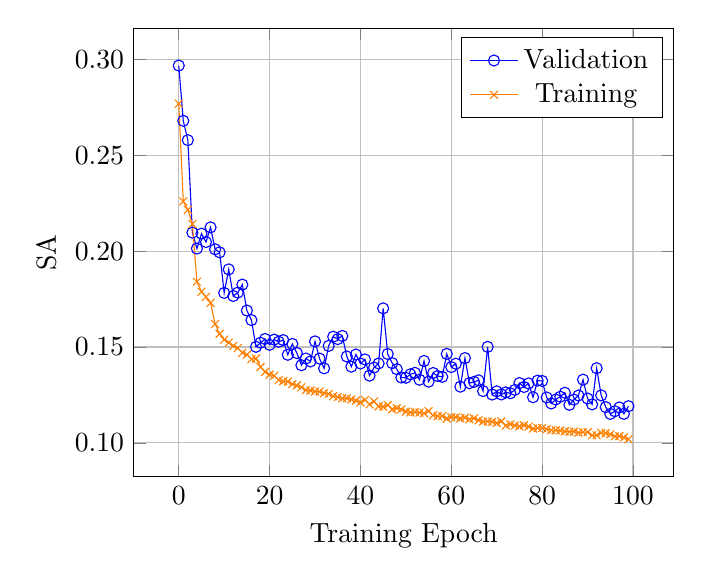
\begin{tikzpicture}
            \begin{axis}[
                    xlabel={Training Epoch},
                    ylabel={SA},
                    grid=major,
                    y tick label style={
                            /pgf/number format/.cd,
                            fixed,
                            fixed zerofill,
                            precision=2,
                            /tikz/.cd
                        },
                    x tick label style={
                            /pgf/number format/.cd,
                            fixed,
                            fixed zerofill,
                            precision=0,
                            /tikz/.cd
                        }
                ]

                \addplot [color=blue, mark=o] coordinates {
                        (0, 0.29695960879325867)
                        (1, 0.26811712980270386)
                        (2, 0.258019357919693)
                        (3, 0.2097473442554474)
                        (4, 0.20143432915210724)
                        (5, 0.20919468998908997)
                        (6, 0.2048226296901703)
                        (7, 0.21249204874038696)
                        (8, 0.2010364532470703)
                        (9, 0.19945918023586273)
                        (10, 0.178276926279068)
                        (11, 0.19053958356380463)
                        (12, 0.17665500938892365)
                        (13, 0.1784226894378662)
                        (14, 0.18260015547275543)
                        (15, 0.16906920075416565)
                        (16, 0.16408582031726837)
                        (17, 0.15011030435562134)
                        (18, 0.15225434303283691)
                        (19, 0.15421821177005768)
                        (20, 0.15117022395133972)
                        (21, 0.15387287735939026)
                        (22, 0.15275633335113525)
                        (23, 0.15360882878303528)
                        (24, 0.1459631621837616)
                        (25, 0.15162958204746246)
                        (26, 0.14687387645244598)
                        (27, 0.1405247449874878)
                        (28, 0.14399001002311707)
                        (29, 0.1424819827079773)
                        (30, 0.1529456526041031)
                        (31, 0.14396043121814728)
                        (32, 0.13886715471744537)
                        (33, 0.1506100744009018)
                        (34, 0.15539668500423431)
                        (35, 0.15415368974208832)
                        (36, 0.1557912677526474)
                        (37, 0.14507997035980225)
                        (38, 0.13975995779037476)
                        (39, 0.14609813690185547)
                        (40, 0.14140722155570984)
                        (41, 0.14353637397289276)
                        (42, 0.13505904376506805)
                        (43, 0.13929425179958344)
                        (44, 0.14142081141471863)
                        (45, 0.1702008694410324)
                        (46, 0.1463731825351715)
                        (47, 0.1415833979845047)
                        (48, 0.13843213021755219)
                        (49, 0.13410869240760803)
                        (50, 0.13395462930202484)
                        (51, 0.13577410578727722)
                        (52, 0.1365361362695694)
                        (53, 0.13293614983558655)
                        (54, 0.14271755516529083)
                        (55, 0.13193625211715698)
                        (56, 0.1364619880914688)
                        (57, 0.13488377630710602)
                        (58, 0.1344253271818161)
                        (59, 0.14644156396389008)
                        (60, 0.13953153789043427)
                        (61, 0.14130368828773499)
                        (62, 0.129317969083786)
                        (63, 0.14424282312393188)
                        (64, 0.13112632930278778)
                        (65, 0.13182976841926575)
                        (66, 0.13261516392230988)
                        (67, 0.12700901925563812)
                        (68, 0.15008729696273804)
                        (69, 0.12520059943199158)
                        (70, 0.1268688291311264)
                        (71, 0.12526105344295502)
                        (72, 0.12633980810642242)
                        (73, 0.12586238980293274)
                        (74, 0.12761858105659485)
                        (75, 0.13118979334831238)
                        (76, 0.1291525810956955)
                        (77, 0.13098861277103424)
                        (78, 0.1238001137971878)
                        (79, 0.13247163593769073)
                        (80, 0.1322963535785675)
                        (81, 0.12366344034671783)
                        (82, 0.12054216861724854)
                        (83, 0.12260898947715759)
                        (84, 0.12406525015830994)
                        (85, 0.12612803280353546)
                        (86, 0.11985144019126892)
                        (87, 0.12258632481098175)
                        (88, 0.12469696253538132)
                        (89, 0.13297420740127563)
                        (90, 0.12312987446784973)
                        (91, 0.1200702041387558)
                        (92, 0.13894999027252197)
                        (93, 0.12475647777318954)
                        (94, 0.11864002794027328)
                        (95, 0.11509356647729874)
                        (96, 0.11647109687328339)
                        (97, 0.11846987903118134)
                        (98, 0.1151323989033699)
                        (99, 0.11911172419786453)
                    };
                \addlegendentry{Validation}

                \addplot [color=orange, mark=x] coordinates {
                        (0, 0.27714234590530396)
                        (1, 0.22605125606060028)
                        (2, 0.22166603803634644)
                        (3, 0.2142174392938614)
                        (4, 0.18410977721214294)
                        (5, 0.17891420423984528)
                        (6, 0.176164910197258)
                        (7, 0.17310594022274017)
                        (8, 0.16203489899635315)
                        (9, 0.15687143802642822)
                        (10, 0.15385130047798157)
                        (11, 0.15230987966060638)
                        (12, 0.15059885382652283)
                        (13, 0.14945240318775177)
                        (14, 0.1470097452402115)
                        (15, 0.14606209099292755)
                        (16, 0.14370131492614746)
                        (17, 0.14400124549865723)
                        (18, 0.1396026462316513)
                        (19, 0.13699065148830414)
                        (20, 0.13558830320835114)
                        (21, 0.135020449757576)
                        (22, 0.13273315131664276)
                        (23, 0.1321326494216919)
                        (24, 0.13190092146396637)
                        (25, 0.13061971962451935)
                        (26, 0.1299782693386078)
                        (27, 0.12900950014591217)
                        (28, 0.12754637002944946)
                        (29, 0.12729746103286743)
                        (30, 0.1267848014831543)
                        (31, 0.12673434615135193)
                        (32, 0.12588557600975037)
                        (33, 0.12545540928840637)
                        (34, 0.12436310946941376)
                        (35, 0.12387336790561676)
                        (36, 0.12326203286647797)
                        (37, 0.12326817214488983)
                        (38, 0.12263922393321991)
                        (39, 0.12206120043992996)
                        (40, 0.12106367945671082)
                        (41, 0.12239518016576767)
                        (42, 0.12005365639925003)
                        (43, 0.12163573503494263)
                        (44, 0.11903729289770126)
                        (45, 0.11888808757066727)
                        (46, 0.11971043050289154)
                        (47, 0.117518849670887)
                        (48, 0.11805302649736404)
                        (49, 0.11745434999465942)
                        (50, 0.11627041548490524)
                        (51, 0.11587575078010559)
                        (52, 0.11607635766267776)
                        (53, 0.11576247960329056)
                        (54, 0.1154271736741066)
                        (55, 0.11651692539453506)
                        (56, 0.11435338109731674)
                        (57, 0.11396262794733047)
                        (58, 0.11386863142251968)
                        (59, 0.11269258707761765)
                        (60, 0.11337878555059433)
                        (61, 0.11333566159009933)
                        (62, 0.11275861412286758)
                        (63, 0.11313185840845108)
                        (64, 0.11220846325159073)
                        (65, 0.11279542744159698)
                        (66, 0.11176317930221558)
                        (67, 0.11107277125120163)
                        (68, 0.1111292839050293)
                        (69, 0.11097381263971329)
                        (70, 0.1103489100933075)
                        (71, 0.11114624887704849)
                        (72, 0.10904093086719513)
                        (73, 0.10972408950328827)
                        (74, 0.10903487354516983)
                        (75, 0.10862037539482117)
                        (76, 0.10915154963731766)
                        (77, 0.10850829631090164)
                        (78, 0.10744006186723709)
                        (79, 0.10773684829473495)
                        (80, 0.1077406033873558)
                        (81, 0.1070765033364296)
                        (82, 0.10663444548845291)
                        (83, 0.10656753927469254)
                        (84, 0.10635998845100403)
                        (85, 0.10595720261335373)
                        (86, 0.10576187819242477)
                        (87, 0.10586992651224136)
                        (88, 0.10534753650426865)
                        (89, 0.10557933151721954)
                        (90, 0.10556600987911224)
                        (91, 0.10395386815071106)
                        (92, 0.10394113510847092)
                        (93, 0.10519018769264221)
                        (94, 0.10500438511371613)
                        (95, 0.10440074652433395)
                        (96, 0.10340135544538498)
                        (97, 0.10348878055810928)
                        (98, 0.10279275476932526)
                        (99, 0.10189473628997803)
                    };
                \addlegendentry{Training}

            \end{axis}
        \end{tikzpicture}
        \caption{SA over Epochs}
        \label{fig:sa_mid_rcgdnae}
    \end{subfigure}
    \hfill
    \begin{subfigure}{0.45\textwidth}
        \centering
        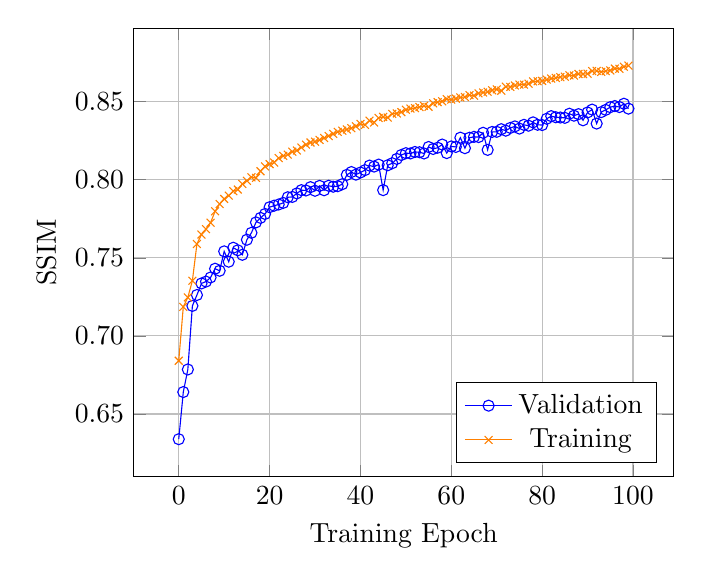
\begin{tikzpicture}
            \begin{axis}[
                    legend pos = south east,
                    xlabel={Training Epoch},
                    ylabel={SSIM},
                    grid=major,
                    y tick label style={
                            /pgf/number format/.cd,
                            fixed,
                            fixed zerofill,
                            precision=2,
                            /tikz/.cd
                        },
                    x tick label style={
                            /pgf/number format/.cd,
                            fixed,
                            fixed zerofill,
                            precision=0,
                            /tikz/.cd
                        }
                ]

                \addplot [color=blue, mark=o] coordinates {
                        (0, 0.633901059627533)
                        (1, 0.6640783548355103)
                        (2, 0.6785396337509155)
                        (3, 0.7192418575286865)
                        (4, 0.7262119650840759)
                        (5, 0.7336249947547913)
                        (6, 0.7348182797431946)
                        (7, 0.7374337911605835)
                        (8, 0.7430384755134583)
                        (9, 0.7417275309562683)
                        (10, 0.7541558146476746)
                        (11, 0.7475339770317078)
                        (12, 0.756472110748291)
                        (13, 0.7548457384109497)
                        (14, 0.7519635558128357)
                        (15, 0.7616060972213745)
                        (16, 0.7660409212112427)
                        (17, 0.7727125883102417)
                        (18, 0.7756003141403198)
                        (19, 0.7781081199645996)
                        (20, 0.7824438214302063)
                        (21, 0.783403754234314)
                        (22, 0.7841631174087524)
                        (23, 0.7851884961128235)
                        (24, 0.7888023853302002)
                        (25, 0.7890048027038574)
                        (26, 0.7912712097167969)
                        (27, 0.7933455109596252)
                        (28, 0.7931289672851562)
                        (29, 0.7952576279640198)
                        (30, 0.7929524183273315)
                        (31, 0.7960907220840454)
                        (32, 0.7932851910591125)
                        (33, 0.7961452007293701)
                        (34, 0.7955543994903564)
                        (35, 0.7958796620368958)
                        (36, 0.7971485257148743)
                        (37, 0.8031440377235413)
                        (38, 0.8049437999725342)
                        (39, 0.8032834529876709)
                        (40, 0.8046506643295288)
                        (41, 0.8061700463294983)
                        (42, 0.8090693950653076)
                        (43, 0.8084341883659363)
                        (44, 0.8096952438354492)
                        (45, 0.7933670878410339)
                        (46, 0.809275209903717)
                        (47, 0.8105871081352234)
                        (48, 0.8133543729782104)
                        (49, 0.8158474564552307)
                        (50, 0.8170235753059387)
                        (51, 0.8168525099754333)
                        (52, 0.8177925944328308)
                        (53, 0.8176009058952332)
                        (54, 0.8168330788612366)
                        (55, 0.8209725618362427)
                        (56, 0.8197097182273865)
                        (57, 0.8205276131629944)
                        (58, 0.8225321173667908)
                        (59, 0.8170779943466187)
                        (60, 0.821334958076477)
                        (61, 0.821007251739502)
                        (62, 0.8269540667533875)
                        (63, 0.8202301859855652)
                        (64, 0.8269054293632507)
                        (65, 0.8274623155593872)
                        (66, 0.8273440003395081)
                        (67, 0.8300628066062927)
                        (68, 0.8191337585449219)
                        (69, 0.8306341171264648)
                        (70, 0.8307029604911804)
                        (71, 0.832369327545166)
                        (72, 0.8314300775527954)
                        (73, 0.8332024216651917)
                        (74, 0.8341630697250366)
                        (75, 0.8327726125717163)
                        (76, 0.8351647257804871)
                        (77, 0.8346092104911804)
                        (78, 0.8367351293563843)
                        (79, 0.8352075815200806)
                        (80, 0.8350265026092529)
                        (81, 0.8390578627586365)
                        (82, 0.8407236933708191)
                        (83, 0.840009868144989)
                        (84, 0.8398355841636658)
                        (85, 0.8396422863006592)
                        (86, 0.8422750234603882)
                        (87, 0.8410248160362244)
                        (88, 0.8420149087905884)
                        (89, 0.8380787372589111)
                        (90, 0.8431065082550049)
                        (91, 0.8449128866195679)
                        (92, 0.8359887003898621)
                        (93, 0.843311071395874)
                        (94, 0.8447472453117371)
                        (95, 0.8464663028717041)
                        (96, 0.8472007513046265)
                        (97, 0.8465434312820435)
                        (98, 0.8486641645431519)
                        (99, 0.8455368280410767)
                    };
                \addlegendentry{Validation}

                \addplot [color=orange, mark=x] coordinates {
                        (0, 0.6841077208518982)
                        (1, 0.7186378836631775)
                        (2, 0.7246882319450378)
                        (3, 0.7353276014328003)
                        (4, 0.7588842511177063)
                        (5, 0.7649483680725098)
                        (6, 0.7684009075164795)
                        (7, 0.7724849581718445)
                        (8, 0.7798029184341431)
                        (9, 0.7844671010971069)
                        (10, 0.7877391576766968)
                        (11, 0.789849042892456)
                        (12, 0.7926805019378662)
                        (13, 0.7937393188476562)
                        (14, 0.7973210215568542)
                        (15, 0.7993070483207703)
                        (16, 0.8016031384468079)
                        (17, 0.8012195229530334)
                        (18, 0.805454671382904)
                        (19, 0.8085289001464844)
                        (20, 0.8100268244743347)
                        (21, 0.8110153079032898)
                        (22, 0.8138625621795654)
                        (23, 0.815289318561554)
                        (24, 0.8161004185676575)
                        (25, 0.817976176738739)
                        (26, 0.8187304139137268)
                        (27, 0.8206737637519836)
                        (28, 0.8224731087684631)
                        (29, 0.823866069316864)
                        (30, 0.8243982195854187)
                        (31, 0.8255012631416321)
                        (32, 0.8267053961753845)
                        (33, 0.8279934525489807)
                        (34, 0.8294117450714111)
                        (35, 0.8306745886802673)
                        (36, 0.8314477801322937)
                        (37, 0.83219975233078)
                        (38, 0.8330261707305908)
                        (39, 0.8342434167861938)
                        (40, 0.8357520699501038)
                        (41, 0.8351477980613708)
                        (42, 0.8378384113311768)
                        (43, 0.8366886973381042)
                        (44, 0.8395704030990601)
                        (45, 0.8402524590492249)
                        (46, 0.839848518371582)
                        (47, 0.8421758413314819)
                        (48, 0.8424451351165771)
                        (49, 0.8433243036270142)
                        (50, 0.844814121723175)
                        (51, 0.8455648422241211)
                        (52, 0.8458409309387207)
                        (53, 0.8465591669082642)
                        (54, 0.8473159670829773)
                        (55, 0.8467060327529907)
                        (56, 0.8489314913749695)
                        (57, 0.8496918082237244)
                        (58, 0.8502432107925415)
                        (59, 0.8516241908073425)
                        (60, 0.8513229489326477)
                        (61, 0.8519449234008789)
                        (62, 0.8527113199234009)
                        (63, 0.8530081510543823)
                        (64, 0.8541745543479919)
                        (65, 0.8538423776626587)
                        (66, 0.8553232550621033)
                        (67, 0.8558663725852966)
                        (68, 0.856341540813446)
                        (69, 0.8572643995285034)
                        (70, 0.8578663468360901)
                        (71, 0.8570104837417603)
                        (72, 0.8595414757728577)
                        (73, 0.8594472408294678)
                        (74, 0.8603616952896118)
                        (75, 0.860916793346405)
                        (76, 0.8609113693237305)
                        (77, 0.8614994287490845)
                        (78, 0.8629931807518005)
                        (79, 0.8630707263946533)
                        (80, 0.863288164138794)
                        (81, 0.8641133904457092)
                        (82, 0.8648011088371277)
                        (83, 0.8651711344718933)
                        (84, 0.8657117486000061)
                        (85, 0.8659795522689819)
                        (86, 0.8668912053108215)
                        (87, 0.8667005300521851)
                        (88, 0.867730438709259)
                        (89, 0.8677107095718384)
                        (90, 0.8678808808326721)
                        (91, 0.8695929050445557)
                        (92, 0.8697127103805542)
                        (93, 0.869046688079834)
                        (94, 0.8695196509361267)
                        (95, 0.8699815273284912)
                        (96, 0.8711657524108887)
                        (97, 0.8710355162620544)
                        (98, 0.8723680377006531)
                        (99, 0.8730998635292053)
                    };
                \addlegendentry{Training}

            \end{axis}
        \end{tikzpicture}
        \caption{SSIM over Epochs}
        \label{fig:ssim_mid_rcgdnae}
    \end{subfigure}
    \caption{Training and Validation Metrics over Epochs for RCGDNAE medium bitrate model.}
    \label{fig:training_metrics_rcgdnae_medium}

\end{figure}

% Low
\begin{figure}
    \centering

    \begin{subfigure}{0.45\textwidth}
        \centering
        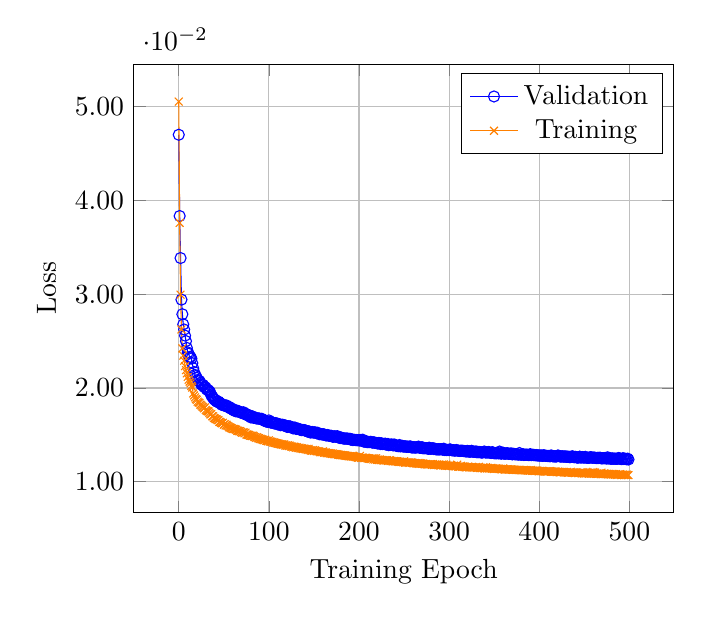
\begin{tikzpicture}
            \begin{axis}[
                    xlabel={Training Epoch},
                    ylabel={Loss},
                    grid=major,
                    y tick label style={
                            /pgf/number format/.cd,
                            fixed,
                            fixed zerofill,
                            precision=2,
                            /tikz/.cd
                        },
                    x tick label style={
                            /pgf/number format/.cd,
                            fixed,
                            fixed zerofill,
                            precision=0,
                            /tikz/.cd
                        }
                ]

                \addplot [color=blue, mark=o] coordinates {
                        (0, 0.047014400362968445)
                        (1, 0.038346875458955765)
                        (2, 0.03386472165584564)
                        (3, 0.02942708320915699)
                        (4, 0.0278711449354887)
                        (5, 0.026791004464030266)
                        (6, 0.02624133974313736)
                        (7, 0.025591980665922165)
                        (8, 0.02500399574637413)
                        (9, 0.02428007684648037)
                        (10, 0.023801449686288834)
                        (11, 0.02365492656826973)
                        (12, 0.023310789838433266)
                        (13, 0.02331247739493847)
                        (14, 0.023141423240303993)
                        (15, 0.022653630003333092)
                        (16, 0.022114932537078857)
                        (17, 0.021709639579057693)
                        (18, 0.021398555487394333)
                        (19, 0.021272791549563408)
                        (20, 0.021078424528241158)
                        (21, 0.020864464342594147)
                        (22, 0.02079080045223236)
                        (23, 0.020745662972331047)
                        (24, 0.020562181249260902)
                        (25, 0.020381873473525047)
                        (26, 0.020319437608122826)
                        (27, 0.020325858145952225)
                        (28, 0.020122341811656952)
                        (29, 0.020118964836001396)
                        (30, 0.02002425491809845)
                        (31, 0.01986142247915268)
                        (32, 0.01979741081595421)
                        (33, 0.019750425592064857)
                        (34, 0.0196364838629961)
                        (35, 0.019514750689268112)
                        (36, 0.01922439970076084)
                        (37, 0.01910213753581047)
                        (38, 0.018958013504743576)
                        (39, 0.01882181316614151)
                        (40, 0.018746303394436836)
                        (41, 0.018693746998906136)
                        (42, 0.01856888271868229)
                        (43, 0.01850758120417595)
                        (44, 0.018559755757451057)
                        (45, 0.018450260162353516)
                        (46, 0.018389470875263214)
                        (47, 0.018308058381080627)
                        (48, 0.018196972087025642)
                        (49, 0.01818842627108097)
                        (50, 0.01813986711204052)
                        (51, 0.018164150416851044)
                        (52, 0.01809675805270672)
                        (53, 0.018145181238651276)
                        (54, 0.017998529598116875)
                        (55, 0.01799660548567772)
                        (56, 0.01798263005912304)
                        (57, 0.017844369634985924)
                        (58, 0.017792511731386185)
                        (59, 0.01780756749212742)
                        (60, 0.01773534156382084)
                        (61, 0.017612185329198837)
                        (62, 0.017667051404714584)
                        (63, 0.01752627082169056)
                        (64, 0.017519444227218628)
                        (65, 0.01756575144827366)
                        (66, 0.017548764124512672)
                        (67, 0.017473148182034492)
                        (68, 0.017444398254156113)
                        (69, 0.017361948266625404)
                        (70, 0.017340047284960747)
                        (71, 0.017372917383909225)
                        (72, 0.01740884967148304)
                        (73, 0.01730082556605339)
                        (74, 0.017256902530789375)
                        (75, 0.017130715772509575)
                        (76, 0.017111025750637054)
                        (77, 0.01709739677608013)
                        (78, 0.017100591212511063)
                        (79, 0.017054405063390732)
                        (80, 0.016859902068972588)
                        (81, 0.016912294551730156)
                        (82, 0.01697298139333725)
                        (83, 0.016815347597002983)
                        (84, 0.01685546338558197)
                        (85, 0.016795475035905838)
                        (86, 0.016774173825979233)
                        (87, 0.01673729345202446)
                        (88, 0.016762757673859596)
                        (89, 0.016750777140259743)
                        (90, 0.016713367775082588)
                        (91, 0.016684047877788544)
                        (92, 0.016722869127988815)
                        (93, 0.016647538170218468)
                        (94, 0.01658509485423565)
                        (95, 0.016527388244867325)
                        (96, 0.016458511352539062)
                        (97, 0.0164470374584198)
                        (98, 0.016409164294600487)
                        (99, 0.01638423278927803)
                        (100, 0.01654634438455105)
                        (101, 0.01640380173921585)
                        (102, 0.016308512538671494)
                        (103, 0.01634347252547741)
                        (104, 0.016306981444358826)
                        (105, 0.01629902422428131)
                        (106, 0.016210563480854034)
                        (107, 0.016259517520666122)
                        (108, 0.016204867511987686)
                        (109, 0.016226815059781075)
                        (110, 0.016109587624669075)
                        (111, 0.01614345610141754)
                        (112, 0.016122641041874886)
                        (113, 0.01602933183312416)
                        (114, 0.0160583034157753)
                        (115, 0.016086041927337646)
                        (116, 0.016060367226600647)
                        (117, 0.015988588333129883)
                        (118, 0.016011333093047142)
                        (119, 0.015963660553097725)
                        (120, 0.015860918909311295)
                        (121, 0.01585286110639572)
                        (122, 0.015920041128993034)
                        (123, 0.015898648649454117)
                        (124, 0.015895921736955643)
                        (125, 0.015795700252056122)
                        (126, 0.015776077285408974)
                        (127, 0.015685774385929108)
                        (128, 0.015753230080008507)
                        (129, 0.01578277349472046)
                        (130, 0.015659969300031662)
                        (131, 0.015628967434167862)
                        (132, 0.015647009015083313)
                        (133, 0.015652582049369812)
                        (134, 0.015576210804283619)
                        (135, 0.015565276145935059)
                        (136, 0.015508097596466541)
                        (137, 0.015519944950938225)
                        (138, 0.015519754961133003)
                        (139, 0.0155123146250844)
                        (140, 0.0154887018725276)
                        (141, 0.01544398907572031)
                        (142, 0.015415475703775883)
                        (143, 0.015359107404947281)
                        (144, 0.015348928049206734)
                        (145, 0.01536758616566658)
                        (146, 0.015248050913214684)
                        (147, 0.015283872373402119)
                        (148, 0.015310688875615597)
                        (149, 0.015266338363289833)
                        (150, 0.01524000708013773)
                        (151, 0.015273860655725002)
                        (152, 0.01524543296545744)
                        (153, 0.015178225003182888)
                        (154, 0.015234067104756832)
                        (155, 0.015150885097682476)
                        (156, 0.015070140361785889)
                        (157, 0.01510099321603775)
                        (158, 0.015068970620632172)
                        (159, 0.015067694708704948)
                        (160, 0.015032676048576832)
                        (161, 0.015071099624037743)
                        (162, 0.014999518170952797)
                        (163, 0.014964237809181213)
                        (164, 0.014935999177396297)
                        (165, 0.014984425157308578)
                        (166, 0.014947773888707161)
                        (167, 0.014902777038514614)
                        (168, 0.014888263307511806)
                        (169, 0.01491531077772379)
                        (170, 0.014856613241136074)
                        (171, 0.014799432829022408)
                        (172, 0.014806102029979229)
                        (173, 0.014856903813779354)
                        (174, 0.014812164939939976)
                        (175, 0.01481110043823719)
                        (176, 0.014867016114294529)
                        (177, 0.014736064709722996)
                        (178, 0.014729447662830353)
                        (179, 0.014659540727734566)
                        (180, 0.014729039743542671)
                        (181, 0.01465779822319746)
                        (182, 0.014641094021499157)
                        (183, 0.014606335200369358)
                        (184, 0.014609221369028091)
                        (185, 0.014604439958930016)
                        (186, 0.014605717733502388)
                        (187, 0.01461254432797432)
                        (188, 0.014573183842003345)
                        (189, 0.014568501152098179)
                        (190, 0.014582070522010326)
                        (191, 0.014487266540527344)
                        (192, 0.014539968222379684)
                        (193, 0.01445022877305746)
                        (194, 0.014464395120739937)
                        (195, 0.014474566094577312)
                        (196, 0.014443918131291866)
                        (197, 0.014452280476689339)
                        (198, 0.01442918460816145)
                        (199, 0.014456030912697315)
                        (200, 0.014416495338082314)
                        (201, 0.014408059418201447)
                        (202, 0.014460752718150616)
                        (203, 0.014393018558621407)
                        (204, 0.014491596259176731)
                        (205, 0.014288119040429592)
                        (206, 0.014293995685875416)
                        (207, 0.014274248853325844)
                        (208, 0.014325352385640144)
                        (209, 0.014225482940673828)
                        (210, 0.014252242632210255)
                        (211, 0.014229070395231247)
                        (212, 0.014234009198844433)
                        (213, 0.014263239689171314)
                        (214, 0.01421412918716669)
                        (215, 0.014170203357934952)
                        (216, 0.014207486994564533)
                        (217, 0.014196961186826229)
                        (218, 0.01414377149194479)
                        (219, 0.014144143089652061)
                        (220, 0.014115403406322002)
                        (221, 0.014071714133024216)
                        (222, 0.014143746346235275)
                        (223, 0.014117696322500706)
                        (224, 0.014019453898072243)
                        (225, 0.014103635214269161)
                        (226, 0.014027152210474014)
                        (227, 0.01404033787548542)
                        (228, 0.014026769436895847)
                        (229, 0.014068073593080044)
                        (230, 0.01396517176181078)
                        (231, 0.013978591188788414)
                        (232, 0.014033214189112186)
                        (233, 0.013898917473852634)
                        (234, 0.013949153013527393)
                        (235, 0.01393186952918768)
                        (236, 0.013988074846565723)
                        (237, 0.013921349309384823)
                        (238, 0.013872948475182056)
                        (239, 0.013984989374876022)
                        (240, 0.013909310102462769)
                        (241, 0.013877544552087784)
                        (242, 0.013816776685416698)
                        (243, 0.01381154265254736)
                        (244, 0.01379699632525444)
                        (245, 0.013917249627411366)
                        (246, 0.013772153295576572)
                        (247, 0.013821817934513092)
                        (248, 0.013834983110427856)
                        (249, 0.013753935694694519)
                        (250, 0.01375268679112196)
                        (251, 0.013794112019240856)
                        (252, 0.013748781755566597)
                        (253, 0.013722489587962627)
                        (254, 0.013759703375399113)
                        (255, 0.013719611801207066)
                        (256, 0.013740181922912598)
                        (257, 0.013777476735413074)
                        (258, 0.013668040744960308)
                        (259, 0.013687795028090477)
                        (260, 0.013643523678183556)
                        (261, 0.013698840513825417)
                        (262, 0.013652093708515167)
                        (263, 0.013644758611917496)
                        (264, 0.01367978099733591)
                        (265, 0.01368550956249237)
                        (266, 0.013752046041190624)
                        (267, 0.013632471673190594)
                        (268, 0.013623747043311596)
                        (269, 0.013608276844024658)
                        (270, 0.013695316389203072)
                        (271, 0.013576360419392586)
                        (272, 0.013595282100141048)
                        (273, 0.013571439310908318)
                        (274, 0.013589736074209213)
                        (275, 0.013586754910647869)
                        (276, 0.01355050876736641)
                        (277, 0.013512319885194302)
                        (278, 0.013639998622238636)
                        (279, 0.013513848185539246)
                        (280, 0.013524002395570278)
                        (281, 0.01356692984700203)
                        (282, 0.013576216995716095)
                        (283, 0.013490122742950916)
                        (284, 0.013536900281906128)
                        (285, 0.013469001278281212)
                        (286, 0.0134640634059906)
                        (287, 0.013449401594698429)
                        (288, 0.013473886996507645)
                        (289, 0.013440875336527824)
                        (290, 0.0134728467091918)
                        (291, 0.013477195985615253)
                        (292, 0.013485148549079895)
                        (293, 0.013412046246230602)
                        (294, 0.013528203591704369)
                        (295, 0.013392533175647259)
                        (296, 0.013392651453614235)
                        (297, 0.013387121260166168)
                        (298, 0.013398503884673119)
                        (299, 0.013392736203968525)
                        (300, 0.013375314883887768)
                        (301, 0.013460110872983932)
                        (302, 0.01340375654399395)
                        (303, 0.013360640034079552)
                        (304, 0.01335435826331377)
                        (305, 0.013371075503528118)
                        (306, 0.013315890915691853)
                        (307, 0.013338380493223667)
                        (308, 0.013382074423134327)
                        (309, 0.013334411196410656)
                        (310, 0.013323884457349777)
                        (311, 0.0132956737652421)
                        (312, 0.013288172893226147)
                        (313, 0.013320567086338997)
                        (314, 0.01330308336764574)
                        (315, 0.013301027938723564)
                        (316, 0.013281336054205894)
                        (317, 0.013271144591271877)
                        (318, 0.013256619684398174)
                        (319, 0.013226370327174664)
                        (320, 0.013294951990246773)
                        (321, 0.013220860622823238)
                        (322, 0.01327548548579216)
                        (323, 0.013192112557590008)
                        (324, 0.013228381983935833)
                        (325, 0.013301265425980091)
                        (326, 0.013209504075348377)
                        (327, 0.013206006027758121)
                        (328, 0.01320813037455082)
                        (329, 0.013187873177230358)
                        (330, 0.013232629746198654)
                        (331, 0.013146999292075634)
                        (332, 0.013187425211071968)
                        (333, 0.013156142085790634)
                        (334, 0.013176673091948032)
                        (335, 0.013157493434846401)
                        (336, 0.013107739388942719)
                        (337, 0.013123799115419388)
                        (338, 0.013161715120077133)
                        (339, 0.01322722528129816)
                        (340, 0.013128788210451603)
                        (341, 0.013121386058628559)
                        (342, 0.013149919919669628)
                        (343, 0.013113915920257568)
                        (344, 0.013181240297853947)
                        (345, 0.013117452152073383)
                        (346, 0.013080466538667679)
                        (347, 0.013078475371003151)
                        (348, 0.013162756338715553)
                        (349, 0.01308448612689972)
                        (350, 0.013040777295827866)
                        (351, 0.013057546690106392)
                        (352, 0.013030669651925564)
                        (353, 0.013053498230874538)
                        (354, 0.0130749037489295)
                        (355, 0.01302300114184618)
                        (356, 0.013222439214587212)
                        (357, 0.013028129003942013)
                        (358, 0.012993083335459232)
                        (359, 0.013079104945063591)
                        (360, 0.013099385425448418)
                        (361, 0.012986299581825733)
                        (362, 0.013016623444855213)
                        (363, 0.0129945557564497)
                        (364, 0.013036892749369144)
                        (365, 0.013043850660324097)
                        (366, 0.01297372579574585)
                        (367, 0.012979958206415176)
                        (368, 0.012995067052543163)
                        (369, 0.01302642934024334)
                        (370, 0.012918760068714619)
                        (371, 0.012990601360797882)
                        (372, 0.012969153001904488)
                        (373, 0.012928921729326248)
                        (374, 0.012926911935210228)
                        (375, 0.012942207977175713)
                        (376, 0.012927147559821606)
                        (377, 0.012886912561953068)
                        (378, 0.013064969331026077)
                        (379, 0.012912622652947903)
                        (380, 0.012876729480922222)
                        (381, 0.012908549048006535)
                        (382, 0.012940507382154465)
                        (383, 0.012859408743679523)
                        (384, 0.012881815433502197)
                        (385, 0.012880535796284676)
                        (386, 0.01289615873247385)
                        (387, 0.012875985354185104)
                        (388, 0.012846946716308594)
                        (389, 0.012851941399276257)
                        (390, 0.012944217771291733)
                        (391, 0.012841291725635529)
                        (392, 0.01286472287029028)
                        (393, 0.012884711846709251)
                        (394, 0.01283985748887062)
                        (395, 0.012852503918111324)
                        (396, 0.012819232419133186)
                        (397, 0.012848430313169956)
                        (398, 0.012809785082936287)
                        (399, 0.012799061834812164)
                        (400, 0.0128097515553236)
                        (401, 0.012793549336493015)
                        (402, 0.012782352045178413)
                        (403, 0.012814982794225216)
                        (404, 0.012760556302964687)
                        (405, 0.012825294397771358)
                        (406, 0.012801711447536945)
                        (407, 0.012761238031089306)
                        (408, 0.012764030136168003)
                        (409, 0.012749818153679371)
                        (410, 0.012746414169669151)
                        (411, 0.012752284295856953)
                        (412, 0.012714055366814137)
                        (413, 0.012800062075257301)
                        (414, 0.012786097824573517)
                        (415, 0.01270866859704256)
                        (416, 0.012728498317301273)
                        (417, 0.012698724865913391)
                        (418, 0.012708858586847782)
                        (419, 0.012688041664659977)
                        (420, 0.012762476690113544)
                        (421, 0.012806938029825687)
                        (422, 0.012727693654596806)
                        (423, 0.012723547406494617)
                        (424, 0.012679887935519218)
                        (425, 0.012699078768491745)
                        (426, 0.012725135311484337)
                        (427, 0.012677331455051899)
                        (428, 0.012683030217885971)
                        (429, 0.012709377333521843)
                        (430, 0.01265848521143198)
                        (431, 0.012687462382018566)
                        (432, 0.012652148492634296)
                        (433, 0.012667720206081867)
                        (434, 0.012615414336323738)
                        (435, 0.0126700010150671)
                        (436, 0.012667456641793251)
                        (437, 0.012718863785266876)
                        (438, 0.01264199335128069)
                        (439, 0.012618794105947018)
                        (440, 0.012661629356443882)
                        (441, 0.012629135511815548)
                        (442, 0.01256994903087616)
                        (443, 0.012589788995683193)
                        (444, 0.012587888166308403)
                        (445, 0.012683505192399025)
                        (446, 0.012576291337609291)
                        (447, 0.012598088011145592)
                        (448, 0.012634853832423687)
                        (449, 0.01258245762437582)
                        (450, 0.012580834329128265)
                        (451, 0.012656950391829014)
                        (452, 0.012568776495754719)
                        (453, 0.01258076075464487)
                        (454, 0.012556774541735649)
                        (455, 0.012554406188428402)
                        (456, 0.012576641514897346)
                        (457, 0.012628979980945587)
                        (458, 0.012589064426720142)
                        (459, 0.012564136646687984)
                        (460, 0.012579835951328278)
                        (461, 0.012574913911521435)
                        (462, 0.012563751079142094)
                        (463, 0.012534166686236858)
                        (464, 0.012523407116532326)
                        (465, 0.012556321918964386)
                        (466, 0.01253588031977415)
                        (467, 0.012560608796775341)
                        (468, 0.012549996376037598)
                        (469, 0.012490106746554375)
                        (470, 0.012519925832748413)
                        (471, 0.012500018812716007)
                        (472, 0.012529637664556503)
                        (473, 0.01249959971755743)
                        (474, 0.012550994753837585)
                        (475, 0.012466845102608204)
                        (476, 0.01260689739137888)
                        (477, 0.012487283907830715)
                        (478, 0.01252372283488512)
                        (479, 0.012459831312298775)
                        (480, 0.012454809620976448)
                        (481, 0.01249992661178112)
                        (482, 0.012442686595022678)
                        (483, 0.012472685426473618)
                        (484, 0.012465129606425762)
                        (485, 0.012449389323592186)
                        (486, 0.012453285045921803)
                        (487, 0.012452976778149605)
                        (488, 0.012531631626188755)
                        (489, 0.012505976483225822)
                        (490, 0.012439383193850517)
                        (491, 0.01242075115442276)
                        (492, 0.012433559633791447)
                        (493, 0.012520345859229565)
                        (494, 0.01243126392364502)
                        (495, 0.012462439015507698)
                        (496, 0.012432359158992767)
                        (497, 0.01239212229847908)
                        (498, 0.012469952926039696)
                        (499, 0.012376605533063412)
                    };
                \addlegendentry{Validation}

                \addplot [color=orange, mark=x] coordinates {
                        (0, 0.050555240362882614)
                        (1, 0.037608593702316284)
                        (2, 0.029958538711071014)
                        (3, 0.02624310925602913)
                        (4, 0.024228451773524284)
                        (5, 0.023453839123249054)
                        (6, 0.02291148714721203)
                        (7, 0.022336319088935852)
                        (8, 0.021906772628426552)
                        (9, 0.02156817726790905)
                        (10, 0.021191008388996124)
                        (11, 0.020892251282930374)
                        (12, 0.02067699283361435)
                        (13, 0.02049317955970764)
                        (14, 0.020228244364261627)
                        (15, 0.02005828730762005)
                        (16, 0.019424762576818466)
                        (17, 0.01920892857015133)
                        (18, 0.019005656242370605)
                        (19, 0.01882554031908512)
                        (20, 0.018746357411146164)
                        (21, 0.018547851592302322)
                        (22, 0.018457531929016113)
                        (23, 0.018414514139294624)
                        (24, 0.018234385177493095)
                        (25, 0.018147021532058716)
                        (26, 0.018037255853414536)
                        (27, 0.017946889623999596)
                        (28, 0.01782739721238613)
                        (29, 0.01793016493320465)
                        (30, 0.01766609214246273)
                        (31, 0.01757199503481388)
                        (32, 0.01753339357674122)
                        (33, 0.01749413087964058)
                        (34, 0.01732778176665306)
                        (35, 0.017197860404849052)
                        (36, 0.01720014028251171)
                        (37, 0.016991013661026955)
                        (38, 0.01698138564825058)
                        (39, 0.01681123487651348)
                        (40, 0.01675686426460743)
                        (41, 0.01668059639632702)
                        (42, 0.016669338569045067)
                        (43, 0.016570426523685455)
                        (44, 0.01656663604080677)
                        (45, 0.01640239544212818)
                        (46, 0.016373571008443832)
                        (47, 0.016282813623547554)
                        (48, 0.016230303794145584)
                        (49, 0.01629527471959591)
                        (50, 0.016086189076304436)
                        (51, 0.016139885410666466)
                        (52, 0.01600145921111107)
                        (53, 0.016086814925074577)
                        (54, 0.015972837805747986)
                        (55, 0.0159219391644001)
                        (56, 0.015813486650586128)
                        (57, 0.01579662598669529)
                        (58, 0.0157381072640419)
                        (59, 0.015683677047491074)
                        (60, 0.015631647780537605)
                        (61, 0.015635360032320023)
                        (62, 0.015619589015841484)
                        (63, 0.015579831786453724)
                        (64, 0.01553963404148817)
                        (65, 0.015424315817654133)
                        (66, 0.01543965470045805)
                        (67, 0.015385405160486698)
                        (68, 0.015403781086206436)
                        (69, 0.015324223786592484)
                        (70, 0.01522912085056305)
                        (71, 0.015270723961293697)
                        (72, 0.015265115536749363)
                        (73, 0.015167958103120327)
                        (74, 0.015232274308800697)
                        (75, 0.01504012756049633)
                        (76, 0.015039822086691856)
                        (77, 0.015003571286797523)
                        (78, 0.01499314047396183)
                        (79, 0.014910949394106865)
                        (80, 0.014905876480042934)
                        (81, 0.014869842678308487)
                        (82, 0.014926320873200893)
                        (83, 0.014879883266985416)
                        (84, 0.014770743437111378)
                        (85, 0.014765576459467411)
                        (86, 0.01468169316649437)
                        (87, 0.014754795469343662)
                        (88, 0.014643439091742039)
                        (89, 0.01464065071195364)
                        (90, 0.014566774480044842)
                        (91, 0.014580242335796356)
                        (92, 0.014520213939249516)
                        (93, 0.01451308187097311)
                        (94, 0.01445228885859251)
                        (95, 0.014432346448302269)
                        (96, 0.01449640467762947)
                        (97, 0.014383850619196892)
                        (98, 0.014363360591232777)
                        (99, 0.014316556043922901)
                        (100, 0.014428632333874702)
                        (101, 0.014292653650045395)
                        (102, 0.014284458011388779)
                        (103, 0.014250405132770538)
                        (104, 0.014260586351156235)
                        (105, 0.014168764464557171)
                        (106, 0.01419941894710064)
                        (107, 0.014144934713840485)
                        (108, 0.01412759069353342)
                        (109, 0.014097906649112701)
                        (110, 0.014072235673666)
                        (111, 0.014052764512598515)
                        (112, 0.014015797525644302)
                        (113, 0.014006038196384907)
                        (114, 0.013978838920593262)
                        (115, 0.013988323509693146)
                        (116, 0.013939142227172852)
                        (117, 0.013991893269121647)
                        (118, 0.01386562455445528)
                        (119, 0.013881952501833439)
                        (120, 0.013837827369570732)
                        (121, 0.013886254280805588)
                        (122, 0.013809839263558388)
                        (123, 0.013861034065485)
                        (124, 0.013797399587929249)
                        (125, 0.013747288845479488)
                        (126, 0.013759407214820385)
                        (127, 0.013674101792275906)
                        (128, 0.013741947710514069)
                        (129, 0.013699867762625217)
                        (130, 0.013636138290166855)
                        (131, 0.013690727762877941)
                        (132, 0.013610350899398327)
                        (133, 0.013586301356554031)
                        (134, 0.013642610050737858)
                        (135, 0.013543020002543926)
                        (136, 0.013589910231530666)
                        (137, 0.013548050075769424)
                        (138, 0.013500136323273182)
                        (139, 0.013536588288843632)
                        (140, 0.013499526306986809)
                        (141, 0.013453683815896511)
                        (142, 0.013500348664820194)
                        (143, 0.013389473780989647)
                        (144, 0.013514388352632523)
                        (145, 0.013385049067437649)
                        (146, 0.01336340419948101)
                        (147, 0.013334044255316257)
                        (148, 0.013324249535799026)
                        (149, 0.013386284001171589)
                        (150, 0.013282684609293938)
                        (151, 0.013361332938075066)
                        (152, 0.013289283961057663)
                        (153, 0.013248119503259659)
                        (154, 0.013237908482551575)
                        (155, 0.013268557377159595)
                        (156, 0.013233162462711334)
                        (157, 0.013155994936823845)
                        (158, 0.013167147524654865)
                        (159, 0.013176345266401768)
                        (160, 0.013225413858890533)
                        (161, 0.013105930760502815)
                        (162, 0.013101741671562195)
                        (163, 0.01313339825719595)
                        (164, 0.013061759993433952)
                        (165, 0.013052527792751789)
                        (166, 0.013053547590970993)
                        (167, 0.013051445595920086)
                        (168, 0.013015753589570522)
                        (169, 0.013023419305682182)
                        (170, 0.012969053350389004)
                        (171, 0.013009080663323402)
                        (172, 0.012951578944921494)
                        (173, 0.0129369106143713)
                        (174, 0.012951986864209175)
                        (175, 0.012938091531395912)
                        (176, 0.012941901572048664)
                        (177, 0.012877749279141426)
                        (178, 0.01289171352982521)
                        (179, 0.01284235343337059)
                        (180, 0.01285850815474987)
                        (181, 0.01283170748502016)
                        (182, 0.012834166176617146)
                        (183, 0.012820310890674591)
                        (184, 0.012816209346055984)
                        (185, 0.012775415554642677)
                        (186, 0.012771799229085445)
                        (187, 0.012768620625138283)
                        (188, 0.012745069339871407)
                        (189, 0.012725651264190674)
                        (190, 0.012740378268063068)
                        (191, 0.0126946484670043)
                        (192, 0.012761545367538929)
                        (193, 0.012676974758505821)
                        (194, 0.012696750462055206)
                        (195, 0.012679836712777615)
                        (196, 0.012648611329495907)
                        (197, 0.012627169489860535)
                        (198, 0.012617816217243671)
                        (199, 0.012575739994645119)
                        (200, 0.012587443925440311)
                        (201, 0.012760364450514317)
                        (202, 0.012541881762444973)
                        (203, 0.01257958821952343)
                        (204, 0.012586495839059353)
                        (205, 0.01254317071288824)
                        (206, 0.012518352828919888)
                        (207, 0.012562952935695648)
                        (208, 0.012555153109133244)
                        (209, 0.012514468282461166)
                        (210, 0.012489587999880314)
                        (211, 0.01245153322815895)
                        (212, 0.012453692965209484)
                        (213, 0.012454583309590816)
                        (214, 0.012420768849551678)
                        (215, 0.012524020858108997)
                        (216, 0.012376702390611172)
                        (217, 0.012502252124249935)
                        (218, 0.012360544875264168)
                        (219, 0.012499873526394367)
                        (220, 0.012344587594270706)
                        (221, 0.012361325323581696)
                        (222, 0.012320373207330704)
                        (223, 0.012383398599922657)
                        (224, 0.012294871732592583)
                        (225, 0.012326635420322418)
                        (226, 0.012313231825828552)
                        (227, 0.012271628715097904)
                        (228, 0.012275626882910728)
                        (229, 0.012303384952247143)
                        (230, 0.01228332705795765)
                        (231, 0.01230042427778244)
                        (232, 0.012221072800457478)
                        (233, 0.012247101403772831)
                        (234, 0.012310883030295372)
                        (235, 0.012198401615023613)
                        (236, 0.012236256152391434)
                        (237, 0.01219168584793806)
                        (238, 0.012170146219432354)
                        (239, 0.012215573340654373)
                        (240, 0.01218104176223278)
                        (241, 0.012181813828647137)
                        (242, 0.012195159681141376)
                        (243, 0.012152076698839664)
                        (244, 0.012111151590943336)
                        (245, 0.012157684192061424)
                        (246, 0.01211626548320055)
                        (247, 0.01210663840174675)
                        (248, 0.012125440873205662)
                        (249, 0.012078090570867062)
                        (250, 0.012181034311652184)
                        (251, 0.012039516121149063)
                        (252, 0.012051721103489399)
                        (253, 0.012071090750396252)
                        (254, 0.012053286656737328)
                        (255, 0.012067459523677826)
                        (256, 0.01200795080512762)
                        (257, 0.012057503685355186)
                        (258, 0.012062513269484043)
                        (259, 0.012029726058244705)
                        (260, 0.01200145110487938)
                        (261, 0.011976069770753384)
                        (262, 0.011998140253126621)
                        (263, 0.011954087764024734)
                        (264, 0.011966342106461525)
                        (265, 0.011932465247809887)
                        (266, 0.012001224793493748)
                        (267, 0.011907115578651428)
                        (268, 0.011986307799816132)
                        (269, 0.01195336040109396)
                        (270, 0.011909859254956245)
                        (271, 0.011943005956709385)
                        (272, 0.01189725287258625)
                        (273, 0.011858949437737465)
                        (274, 0.01188737154006958)
                        (275, 0.011868976056575775)
                        (276, 0.011836526915431023)
                        (277, 0.011868330650031567)
                        (278, 0.011850493028759956)
                        (279, 0.01186728198081255)
                        (280, 0.01187815610319376)
                        (281, 0.011808795854449272)
                        (282, 0.011893381364643574)
                        (283, 0.011788282543420792)
                        (284, 0.011825965717434883)
                        (285, 0.011797784827649593)
                        (286, 0.011801629327237606)
                        (287, 0.011821966618299484)
                        (288, 0.011766740120947361)
                        (289, 0.011813842691481113)
                        (290, 0.011735784821212292)
                        (291, 0.01175878755748272)
                        (292, 0.01183481328189373)
                        (293, 0.011740935035049915)
                        (294, 0.01185648888349533)
                        (295, 0.01170435268431902)
                        (296, 0.011702468618750572)
                        (297, 0.011831746436655521)
                        (298, 0.011709310114383698)
                        (299, 0.01172187365591526)
                        (300, 0.011678704991936684)
                        (301, 0.011781159788370132)
                        (302, 0.01172590907663107)
                        (303, 0.011712001636624336)
                        (304, 0.011659493669867516)
                        (305, 0.011713141575455666)
                        (306, 0.011655728332698345)
                        (307, 0.01165910717099905)
                        (308, 0.011647664941847324)
                        (309, 0.011828717775642872)
                        (310, 0.011601584032177925)
                        (311, 0.011616433039307594)
                        (312, 0.011605549603700638)
                        (313, 0.01169425155967474)
                        (314, 0.01158757135272026)
                        (315, 0.011631863191723824)
                        (316, 0.011580100283026695)
                        (317, 0.011626066640019417)
                        (318, 0.01156120840460062)
                        (319, 0.011548181064426899)
                        (320, 0.011558662168681622)
                        (321, 0.011619534343481064)
                        (322, 0.011539042927324772)
                        (323, 0.011545158922672272)
                        (324, 0.01156288105994463)
                        (325, 0.01151689700782299)
                        (326, 0.011562145315110683)
                        (327, 0.011537928134202957)
                        (328, 0.011523437686264515)
                        (329, 0.01152887474745512)
                        (330, 0.011569407768547535)
                        (331, 0.011477233842015266)
                        (332, 0.01149872038513422)
                        (333, 0.011589677073061466)
                        (334, 0.011466126888990402)
                        (335, 0.011489453725516796)
                        (336, 0.011446230113506317)
                        (337, 0.011476212181150913)
                        (338, 0.011552268639206886)
                        (339, 0.011441308073699474)
                        (340, 0.011419638060033321)
                        (341, 0.011556785553693771)
                        (342, 0.011418893933296204)
                        (343, 0.011477467603981495)
                        (344, 0.011426969431340694)
                        (345, 0.011425615288317204)
                        (346, 0.011466075666248798)
                        (347, 0.011471526697278023)
                        (348, 0.011394099332392216)
                        (349, 0.011438087560236454)
                        (350, 0.011365711688995361)
                        (351, 0.011408159509301186)
                        (352, 0.01140473410487175)
                        (353, 0.011387679725885391)
                        (354, 0.011380532756447792)
                        (355, 0.011411285027861595)
                        (356, 0.011352157220244408)
                        (357, 0.011383917182683945)
                        (358, 0.01133798435330391)
                        (359, 0.011332152411341667)
                        (360, 0.011419218964874744)
                        (361, 0.011336026713252068)
                        (362, 0.011303401552140713)
                        (363, 0.011327325366437435)
                        (364, 0.011323990300297737)
                        (365, 0.011335445567965508)
                        (366, 0.01130099967122078)
                        (367, 0.011311396025121212)
                        (368, 0.011313555762171745)
                        (369, 0.011311774142086506)
                        (370, 0.011294130235910416)
                        (371, 0.011265590786933899)
                        (372, 0.011291475035250187)
                        (373, 0.011277089826762676)
                        (374, 0.011264098808169365)
                        (375, 0.011263779364526272)
                        (376, 0.01125796977430582)
                        (377, 0.011277209036052227)
                        (378, 0.01124182902276516)
                        (379, 0.01126431580632925)
                        (380, 0.011232464574277401)
                        (381, 0.011223305948078632)
                        (382, 0.011234509758651257)
                        (383, 0.011246026493608952)
                        (384, 0.011224291287362576)
                        (385, 0.011222808621823788)
                        (386, 0.011239276267588139)
                        (387, 0.011197267100214958)
                        (388, 0.011208384297788143)
                        (389, 0.011211348697543144)
                        (390, 0.011183803901076317)
                        (391, 0.011252446100115776)
                        (392, 0.011173101142048836)
                        (393, 0.011187031865119934)
                        (394, 0.011175263673067093)
                        (395, 0.011151653714478016)
                        (396, 0.01119054015725851)
                        (397, 0.011178308166563511)
                        (398, 0.011195441707968712)
                        (399, 0.011130072176456451)
                        (400, 0.011126713827252388)
                        (401, 0.01115309726446867)
                        (402, 0.011130809783935547)
                        (403, 0.011164793744683266)
                        (404, 0.01113799773156643)
                        (405, 0.0110993143171072)
                        (406, 0.01109530683606863)
                        (407, 0.011082610115408897)
                        (408, 0.011124244891107082)
                        (409, 0.01108903344720602)
                        (410, 0.011105348356068134)
                        (411, 0.011123467236757278)
                        (412, 0.011134464293718338)
                        (413, 0.011070296168327332)
                        (414, 0.011088849976658821)
                        (415, 0.011073081754148006)
                        (416, 0.011073713190853596)
                        (417, 0.011076613329350948)
                        (418, 0.011093526147305965)
                        (419, 0.011045046150684357)
                        (420, 0.01103229634463787)
                        (421, 0.011088313534855843)
                        (422, 0.011038093827664852)
                        (423, 0.011010563932359219)
                        (424, 0.011022443883121014)
                        (425, 0.011051269248127937)
                        (426, 0.011038017459213734)
                        (427, 0.01103288121521473)
                        (428, 0.010990990325808525)
                        (429, 0.01100380253046751)
                        (430, 0.010994120500981808)
                        (431, 0.011048362590372562)
                        (432, 0.010962536558508873)
                        (433, 0.010982648469507694)
                        (434, 0.011011616326868534)
                        (435, 0.011059756390750408)
                        (436, 0.010972661897540092)
                        (437, 0.01097057107836008)
                        (438, 0.010969714261591434)
                        (439, 0.01094843354076147)
                        (440, 0.010929311625659466)
                        (441, 0.010959952138364315)
                        (442, 0.0109870545566082)
                        (443, 0.010921702720224857)
                        (444, 0.010935484431684017)
                        (445, 0.010950119234621525)
                        (446, 0.011002878658473492)
                        (447, 0.010892090387642384)
                        (448, 0.011020907200872898)
                        (449, 0.010907735675573349)
                        (450, 0.010874064639210701)
                        (451, 0.010945301502943039)
                        (452, 0.0108955642208457)
                        (453, 0.010932219214737415)
                        (454, 0.010919329710304737)
                        (455, 0.010857424698770046)
                        (456, 0.010965746827423573)
                        (457, 0.01087094284594059)
                        (458, 0.010999455116689205)
                        (459, 0.010866639204323292)
                        (460, 0.011045530438423157)
                        (461, 0.010844294913113117)
                        (462, 0.010974096134305)
                        (463, 0.010843333788216114)
                        (464, 0.010848797857761383)
                        (465, 0.010835088789463043)
                        (466, 0.01087135262787342)
                        (467, 0.01089578215032816)
                        (468, 0.01080658845603466)
                        (469, 0.010960930958390236)
                        (470, 0.010810836218297482)
                        (471, 0.010822351090610027)
                        (472, 0.010887694545090199)
                        (473, 0.010834465734660625)
                        (474, 0.010824717581272125)
                        (475, 0.010839540511369705)
                        (476, 0.010801075026392937)
                        (477, 0.010846384800970554)
                        (478, 0.010790384374558926)
                        (479, 0.010830746032297611)
                        (480, 0.010769038461148739)
                        (481, 0.01083954144269228)
                        (482, 0.0107769425958395)
                        (483, 0.010808657854795456)
                        (484, 0.010761724784970284)
                        (485, 0.01081601157784462)
                        (486, 0.010727337561547756)
                        (487, 0.01075255498290062)
                        (488, 0.010767770931124687)
                        (489, 0.010775605216622353)
                        (490, 0.010828492231667042)
                        (491, 0.010713624767959118)
                        (492, 0.010737848468124866)
                        (493, 0.010774107649922371)
                        (494, 0.010715886019170284)
                        (495, 0.010751962661743164)
                        (496, 0.010705236345529556)
                        (497, 0.010772979818284512)
                        (498, 0.010711224749684334)
                        (499, 0.010706647299230099)
                    };
                \addlegendentry{Training}

            \end{axis}
        \end{tikzpicture}
        \caption{Loss over Epochs}
        \label{fig:loss_low_rcgdnae}
    \end{subfigure}
    \hfill
    \begin{subfigure}{0.45\textwidth}
        \centering
        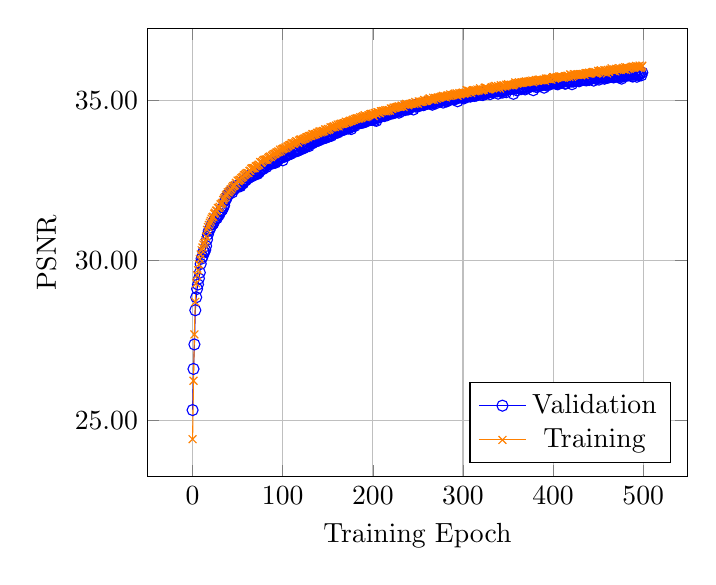
\begin{tikzpicture}
            \begin{axis}[
                    legend pos = south east,
                    xlabel={Training Epoch},
                    ylabel={PSNR},
                    grid=major,
                    y tick label style={
                            /pgf/number format/.cd,
                            fixed,
                            fixed zerofill,
                            precision=2,
                            /tikz/.cd
                        },
                    x tick label style={
                            /pgf/number format/.cd,
                            fixed,
                            fixed zerofill,
                            precision=0,
                            /tikz/.cd
                        }
                ]

                \addplot [color=blue, mark=o] coordinates {
                        (0, 25.330036163330078)
                        (1, 26.614551544189453)
                        (2, 27.380619049072266)
                        (3, 28.448759078979492)
                        (4, 28.853490829467773)
                        (5, 29.11650848388672)
                        (6, 29.254207611083984)
                        (7, 29.4392032623291)
                        (8, 29.62462615966797)
                        (9, 29.897335052490234)
                        (10, 30.061687469482422)
                        (11, 30.119976043701172)
                        (12, 30.280338287353516)
                        (13, 30.259145736694336)
                        (14, 30.332107543945312)
                        (15, 30.455568313598633)
                        (16, 30.65302848815918)
                        (17, 30.816970825195312)
                        (18, 30.92802619934082)
                        (19, 30.978296279907227)
                        (20, 31.040895462036133)
                        (21, 31.129783630371094)
                        (22, 31.135982513427734)
                        (23, 31.156938552856445)
                        (24, 31.23530387878418)
                        (25, 31.298297882080078)
                        (26, 31.335643768310547)
                        (27, 31.32432746887207)
                        (28, 31.42612075805664)
                        (29, 31.419038772583008)
                        (30, 31.460323333740234)
                        (31, 31.543352127075195)
                        (32, 31.575742721557617)
                        (33, 31.591754913330078)
                        (34, 31.65956687927246)
                        (35, 31.723506927490234)
                        (36, 31.8741397857666)
                        (37, 31.918197631835938)
                        (38, 31.971620559692383)
                        (39, 32.04994583129883)
                        (40, 32.07341766357422)
                        (41, 32.09344482421875)
                        (42, 32.15696716308594)
                        (43, 32.184722900390625)
                        (44, 32.12919998168945)
                        (45, 32.20709991455078)
                        (46, 32.232337951660156)
                        (47, 32.24915313720703)
                        (48, 32.321990966796875)
                        (49, 32.30824661254883)
                        (50, 32.339019775390625)
                        (51, 32.318763732910156)
                        (52, 32.34916305541992)
                        (53, 32.32320785522461)
                        (54, 32.40116500854492)
                        (55, 32.40871810913086)
                        (56, 32.410396575927734)
                        (57, 32.48698043823242)
                        (58, 32.511749267578125)
                        (59, 32.504878997802734)
                        (60, 32.544166564941406)
                        (61, 32.60763931274414)
                        (62, 32.57937240600586)
                        (63, 32.65402603149414)
                        (64, 32.6468391418457)
                        (65, 32.62884521484375)
                        (66, 32.639827728271484)
                        (67, 32.662139892578125)
                        (68, 32.6744270324707)
                        (69, 32.7197151184082)
                        (70, 32.73293685913086)
                        (71, 32.71783447265625)
                        (72, 32.70918273925781)
                        (73, 32.74870681762695)
                        (74, 32.766258239746094)
                        (75, 32.833438873291016)
                        (76, 32.850990295410156)
                        (77, 32.86045455932617)
                        (78, 32.85894775390625)
                        (79, 32.88591766357422)
                        (80, 32.99354553222656)
                        (81, 32.96335220336914)
                        (82, 32.92545700073242)
                        (83, 33.00798416137695)
                        (84, 32.99197006225586)
                        (85, 33.01087188720703)
                        (86, 33.03948974609375)
                        (87, 33.04957962036133)
                        (88, 33.03843307495117)
                        (89, 33.04019546508789)
                        (90, 33.062530517578125)
                        (91, 33.07449722290039)
                        (92, 33.05979537963867)
                        (93, 33.09969711303711)
                        (94, 33.12501907348633)
                        (95, 33.16048049926758)
                        (96, 33.19780731201172)
                        (97, 33.212806701660156)
                        (98, 33.22996139526367)
                        (99, 33.23807144165039)
                        (100, 33.13276290893555)
                        (101, 33.235633850097656)
                        (102, 33.286659240722656)
                        (103, 33.26798629760742)
                        (104, 33.28385925292969)
                        (105, 33.29649353027344)
                        (106, 33.346031188964844)
                        (107, 33.31770324707031)
                        (108, 33.329837799072266)
                        (109, 33.338478088378906)
                        (110, 33.3995475769043)
                        (111, 33.382301330566406)
                        (112, 33.38982391357422)
                        (113, 33.44874572753906)
                        (114, 33.4358024597168)
                        (115, 33.41803741455078)
                        (116, 33.42464065551758)
                        (117, 33.4655647277832)
                        (118, 33.44684600830078)
                        (119, 33.475677490234375)
                        (120, 33.55447006225586)
                        (121, 33.57177734375)
                        (122, 33.507625579833984)
                        (123, 33.506858825683594)
                        (124, 33.540775299072266)
                        (125, 33.588722229003906)
                        (126, 33.58938217163086)
                        (127, 33.64128112792969)
                        (128, 33.599979400634766)
                        (129, 33.575904846191406)
                        (130, 33.663570404052734)
                        (131, 33.677001953125)
                        (132, 33.6607780456543)
                        (133, 33.66561508178711)
                        (134, 33.702735900878906)
                        (135, 33.71480941772461)
                        (136, 33.74542999267578)
                        (137, 33.74488830566406)
                        (138, 33.73645782470703)
                        (139, 33.749813079833984)
                        (140, 33.75362777709961)
                        (141, 33.78908920288086)
                        (142, 33.79362487792969)
                        (143, 33.83345413208008)
                        (144, 33.84075927734375)
                        (145, 33.813636779785156)
                        (146, 33.908565521240234)
                        (147, 33.874813079833984)
                        (148, 33.839481353759766)
                        (149, 33.883338928222656)
                        (150, 33.902462005615234)
                        (151, 33.87654495239258)
                        (152, 33.893741607666016)
                        (153, 33.920040130615234)
                        (154, 33.899478912353516)
                        (155, 33.95052719116211)
                        (156, 34.00400161743164)
                        (157, 33.978729248046875)
                        (158, 34.001365661621094)
                        (159, 34.00627517700195)
                        (160, 34.00870895385742)
                        (161, 33.99781799316406)
                        (162, 34.04015350341797)
                        (163, 34.06496047973633)
                        (164, 34.097572326660156)
                        (165, 34.06114959716797)
                        (166, 34.07659912109375)
                        (167, 34.09431838989258)
                        (168, 34.10453414916992)
                        (169, 34.10093307495117)
                        (170, 34.12600326538086)
                        (171, 34.18010330200195)
                        (172, 34.17251205444336)
                        (173, 34.12678146362305)
                        (174, 34.163124084472656)
                        (175, 34.16189193725586)
                        (176, 34.1103401184082)
                        (177, 34.20570755004883)
                        (178, 34.21509552001953)
                        (179, 34.27177047729492)
                        (180, 34.206241607666016)
                        (181, 34.271514892578125)
                        (182, 34.279476165771484)
                        (183, 34.29322814941406)
                        (184, 34.29789352416992)
                        (185, 34.29552459716797)
                        (186, 34.297874450683594)
                        (187, 34.30324172973633)
                        (188, 34.31378173828125)
                        (189, 34.31878662109375)
                        (190, 34.319549560546875)
                        (191, 34.3867073059082)
                        (192, 34.33865737915039)
                        (193, 34.41353988647461)
                        (194, 34.39927291870117)
                        (195, 34.38677978515625)
                        (196, 34.40870666503906)
                        (197, 34.399417877197266)
                        (198, 34.39780807495117)
                        (199, 34.40040588378906)
                        (200, 34.42177200317383)
                        (201, 34.42325973510742)
                        (202, 34.38260269165039)
                        (203, 34.44231033325195)
                        (204, 34.3673095703125)
                        (205, 34.50480270385742)
                        (206, 34.495079040527344)
                        (207, 34.497344970703125)
                        (208, 34.48453903198242)
                        (209, 34.55380630493164)
                        (210, 34.53366470336914)
                        (211, 34.53852462768555)
                        (212, 34.539329528808594)
                        (213, 34.51627731323242)
                        (214, 34.546329498291016)
                        (215, 34.57373809814453)
                        (216, 34.544342041015625)
                        (217, 34.573055267333984)
                        (218, 34.59437942504883)
                        (219, 34.58399963378906)
                        (220, 34.6187629699707)
                        (221, 34.65662384033203)
                        (222, 34.599456787109375)
                        (223, 34.62333297729492)
                        (224, 34.68229675292969)
                        (225, 34.62513732910156)
                        (226, 34.67585372924805)
                        (227, 34.664161682128906)
                        (228, 34.67034149169922)
                        (229, 34.622154235839844)
                        (230, 34.7176628112793)
                        (231, 34.70795822143555)
                        (232, 34.672664642333984)
                        (233, 34.765804290771484)
                        (234, 34.72286605834961)
                        (235, 34.749874114990234)
                        (236, 34.706058502197266)
                        (237, 34.7489128112793)
                        (238, 34.7778205871582)
                        (239, 34.7197380065918)
                        (240, 34.74383544921875)
                        (241, 34.77318572998047)
                        (242, 34.82515335083008)
                        (243, 34.82490158081055)
                        (244, 34.8441047668457)
                        (245, 34.72102737426758)
                        (246, 34.85845947265625)
                        (247, 34.828433990478516)
                        (248, 34.80865478515625)
                        (249, 34.88051986694336)
                        (250, 34.87080001831055)
                        (251, 34.824729919433594)
                        (252, 34.860626220703125)
                        (253, 34.888580322265625)
                        (254, 34.862483978271484)
                        (255, 34.887596130371094)
                        (256, 34.85676193237305)
                        (257, 34.86650085449219)
                        (258, 34.917579650878906)
                        (259, 34.905189514160156)
                        (260, 34.94253921508789)
                        (261, 34.90840530395508)
                        (262, 34.93206787109375)
                        (263, 34.92808151245117)
                        (264, 34.899383544921875)
                        (265, 34.90123748779297)
                        (266, 34.870121002197266)
                        (267, 34.94799041748047)
                        (268, 34.951786041259766)
                        (269, 34.95268630981445)
                        (270, 34.914852142333984)
                        (271, 34.988197326660156)
                        (272, 34.978172302246094)
                        (273, 34.995758056640625)
                        (274, 34.964378356933594)
                        (275, 34.98178482055664)
                        (276, 34.99662399291992)
                        (277, 35.03908920288086)
                        (278, 34.93741226196289)
                        (279, 35.02996063232422)
                        (280, 35.0201530456543)
                        (281, 34.983184814453125)
                        (282, 34.97434616088867)
                        (283, 35.037872314453125)
                        (284, 35.00625991821289)
                        (285, 35.06407165527344)
                        (286, 35.053951263427734)
                        (287, 35.08354568481445)
                        (288, 35.042057037353516)
                        (289, 35.07005310058594)
                        (290, 35.05171203613281)
                        (291, 35.05633544921875)
                        (292, 35.04879379272461)
                        (293, 35.08942413330078)
                        (294, 34.97922134399414)
                        (295, 35.10459899902344)
                        (296, 35.10795974731445)
                        (297, 35.10617446899414)
                        (298, 35.101444244384766)
                        (299, 35.094268798828125)
                        (300, 35.11446762084961)
                        (301, 35.06641387939453)
                        (302, 35.09833526611328)
                        (303, 35.12470626831055)
                        (304, 35.132442474365234)
                        (305, 35.122528076171875)
                        (306, 35.162109375)
                        (307, 35.150272369384766)
                        (308, 35.12318801879883)
                        (309, 35.140052795410156)
                        (310, 35.146541595458984)
                        (311, 35.16153335571289)
                        (312, 35.18886947631836)
                        (313, 35.14601516723633)
                        (314, 35.17291259765625)
                        (315, 35.158451080322266)
                        (316, 35.18118667602539)
                        (317, 35.18583297729492)
                        (318, 35.20820617675781)
                        (319, 35.231632232666016)
                        (320, 35.180545806884766)
                        (321, 35.24302291870117)
                        (322, 35.171993255615234)
                        (323, 35.25660705566406)
                        (324, 35.2447624206543)
                        (325, 35.20532989501953)
                        (326, 35.24824523925781)
                        (327, 35.23961639404297)
                        (328, 35.254127502441406)
                        (329, 35.2781982421875)
                        (330, 35.200111389160156)
                        (331, 35.28370666503906)
                        (332, 35.25349807739258)
                        (333, 35.276729583740234)
                        (334, 35.263092041015625)
                        (335, 35.27561950683594)
                        (336, 35.329193115234375)
                        (337, 35.32708740234375)
                        (338, 35.286376953125)
                        (339, 35.21580505371094)
                        (340, 35.301727294921875)
                        (341, 35.322689056396484)
                        (342, 35.28153991699219)
                        (343, 35.295589447021484)
                        (344, 35.24896240234375)
                        (345, 35.3111686706543)
                        (346, 35.33231735229492)
                        (347, 35.33742904663086)
                        (348, 35.26274108886719)
                        (349, 35.34091567993164)
                        (350, 35.3725471496582)
                        (351, 35.366851806640625)
                        (352, 35.372684478759766)
                        (353, 35.36399841308594)
                        (354, 35.367557525634766)
                        (355, 35.39583969116211)
                        (356, 35.21144104003906)
                        (357, 35.374732971191406)
                        (358, 35.40128707885742)
                        (359, 35.37227249145508)
                        (360, 35.31830978393555)
                        (361, 35.404579162597656)
                        (362, 35.39609909057617)
                        (363, 35.41068649291992)
                        (364, 35.37617111206055)
                        (365, 35.36211013793945)
                        (366, 35.42626953125)
                        (367, 35.40388488769531)
                        (368, 35.403953552246094)
                        (369, 35.34975814819336)
                        (370, 35.44889831542969)
                        (371, 35.39073181152344)
                        (372, 35.40787887573242)
                        (373, 35.45415496826172)
                        (374, 35.45246505737305)
                        (375, 35.43879699707031)
                        (376, 35.45295715332031)
                        (377, 35.4857292175293)
                        (378, 35.32469940185547)
                        (379, 35.46077346801758)
                        (380, 35.481658935546875)
                        (381, 35.434913635253906)
                        (382, 35.421260833740234)
                        (383, 35.49494934082031)
                        (384, 35.46889877319336)
                        (385, 35.469051361083984)
                        (386, 35.47383117675781)
                        (387, 35.47391128540039)
                        (388, 35.51346206665039)
                        (389, 35.507625579833984)
                        (390, 35.40352249145508)
                        (391, 35.51121520996094)
                        (392, 35.49459457397461)
                        (393, 35.46989440917969)
                        (394, 35.51968002319336)
                        (395, 35.50164794921875)
                        (396, 35.52903366088867)
                        (397, 35.51238250732422)
                        (398, 35.55210876464844)
                        (399, 35.541786193847656)
                        (400, 35.551910400390625)
                        (401, 35.54648208618164)
                        (402, 35.55434036254883)
                        (403, 35.529815673828125)
                        (404, 35.579490661621094)
                        (405, 35.506996154785156)
                        (406, 35.53392028808594)
                        (407, 35.580230712890625)
                        (408, 35.5826530456543)
                        (409, 35.57799530029297)
                        (410, 35.5902214050293)
                        (411, 35.5732536315918)
                        (412, 35.6209831237793)
                        (413, 35.53038024902344)
                        (414, 35.52995300292969)
                        (415, 35.61864471435547)
                        (416, 35.590675354003906)
                        (417, 35.62516784667969)
                        (418, 35.612308502197266)
                        (419, 35.633792877197266)
                        (420, 35.59524917602539)
                        (421, 35.51155471801758)
                        (422, 35.59446716308594)
                        (423, 35.598052978515625)
                        (424, 35.637245178222656)
                        (425, 35.63197708129883)
                        (426, 35.61808395385742)
                        (427, 35.64845657348633)
                        (428, 35.64970016479492)
                        (429, 35.602054595947266)
                        (430, 35.65293502807617)
                        (431, 35.64088439941406)
                        (432, 35.67207717895508)
                        (433, 35.65973663330078)
                        (434, 35.69819259643555)
                        (435, 35.642704010009766)
                        (436, 35.63959503173828)
                        (437, 35.630706787109375)
                        (438, 35.66642761230469)
                        (439, 35.69575119018555)
                        (440, 35.645381927490234)
                        (441, 35.688026428222656)
                        (442, 35.72726821899414)
                        (443, 35.70868682861328)
                        (444, 35.71554946899414)
                        (445, 35.623634338378906)
                        (446, 35.71167755126953)
                        (447, 35.701416015625)
                        (448, 35.6746711730957)
                        (449, 35.72169494628906)
                        (450, 35.7280158996582)
                        (451, 35.6556510925293)
                        (452, 35.72607421875)
                        (453, 35.72433853149414)
                        (454, 35.72998046875)
                        (455, 35.74305725097656)
                        (456, 35.71748733520508)
                        (457, 35.682884216308594)
                        (458, 35.71249008178711)
                        (459, 35.717830657958984)
                        (460, 35.71317672729492)
                        (461, 35.7275390625)
                        (462, 35.7274055480957)
                        (463, 35.736270904541016)
                        (464, 35.773033142089844)
                        (465, 35.748809814453125)
                        (466, 35.74800109863281)
                        (467, 35.724021911621094)
                        (468, 35.73900604248047)
                        (469, 35.784759521484375)
                        (470, 35.7490234375)
                        (471, 35.78901672363281)
                        (472, 35.75091552734375)
                        (473, 35.75146484375)
                        (474, 35.71909713745117)
                        (475, 35.79419708251953)
                        (476, 35.68537139892578)
                        (477, 35.78749465942383)
                        (478, 35.7592887878418)
                        (479, 35.80220413208008)
                        (480, 35.821048736572266)
                        (481, 35.774444580078125)
                        (482, 35.81611633300781)
                        (483, 35.78557205200195)
                        (484, 35.79785919189453)
                        (485, 35.825618743896484)
                        (486, 35.82487487792969)
                        (487, 35.8084602355957)
                        (488, 35.75220489501953)
                        (489, 35.75872039794922)
                        (490, 35.81867980957031)
                        (491, 35.832889556884766)
                        (492, 35.8185920715332)
                        (493, 35.74456787109375)
                        (494, 35.828983306884766)
                        (495, 35.79905319213867)
                        (496, 35.821937561035156)
                        (497, 35.86035919189453)
                        (498, 35.79014205932617)
                        (499, 35.87477111816406)
                    };
                \addlegendentry{Validation}

                \addplot [color=orange, mark=x] coordinates {
                        (0, 24.419795989990234)
                        (1, 26.245681762695312)
                        (2, 27.693220138549805)
                        (3, 28.71073341369629)
                        (4, 29.291574478149414)
                        (5, 29.544803619384766)
                        (6, 29.701515197753906)
                        (7, 29.883941650390625)
                        (8, 30.050397872924805)
                        (9, 30.192359924316406)
                        (10, 30.324026107788086)
                        (11, 30.408180236816406)
                        (12, 30.502723693847656)
                        (13, 30.555349349975586)
                        (14, 30.63288688659668)
                        (15, 30.749725341796875)
                        (16, 30.958967208862305)
                        (17, 31.04625701904297)
                        (18, 31.115234375)
                        (19, 31.186363220214844)
                        (20, 31.24461555480957)
                        (21, 31.308731079101562)
                        (22, 31.35704231262207)
                        (23, 31.372314453125)
                        (24, 31.464710235595703)
                        (25, 31.497909545898438)
                        (26, 31.558347702026367)
                        (27, 31.562501907348633)
                        (28, 31.64743995666504)
                        (29, 31.645925521850586)
                        (30, 31.68191909790039)
                        (31, 31.756380081176758)
                        (32, 31.77713394165039)
                        (33, 31.80510902404785)
                        (34, 31.89427375793457)
                        (35, 31.944318771362305)
                        (36, 31.98238182067871)
                        (37, 32.040565490722656)
                        (38, 32.07742691040039)
                        (39, 32.139530181884766)
                        (40, 32.13047790527344)
                        (41, 32.17451858520508)
                        (42, 32.21745681762695)
                        (43, 32.23008728027344)
                        (44, 32.284305572509766)
                        (45, 32.32560348510742)
                        (46, 32.331321716308594)
                        (47, 32.36223602294922)
                        (48, 32.42828369140625)
                        (49, 32.405250549316406)
                        (50, 32.498260498046875)
                        (51, 32.47956085205078)
                        (52, 32.52043151855469)
                        (53, 32.531494140625)
                        (54, 32.578773498535156)
                        (55, 32.598018646240234)
                        (56, 32.618568420410156)
                        (57, 32.66397476196289)
                        (58, 32.68164825439453)
                        (59, 32.71202850341797)
                        (60, 32.73675537109375)
                        (61, 32.738258361816406)
                        (62, 32.73261260986328)
                        (63, 32.800148010253906)
                        (64, 32.80946731567383)
                        (65, 32.86943054199219)
                        (66, 32.88523864746094)
                        (67, 32.88689422607422)
                        (68, 32.890716552734375)
                        (69, 32.8896598815918)
                        (70, 32.94318389892578)
                        (71, 32.95757293701172)
                        (72, 32.966026306152344)
                        (73, 32.99437713623047)
                        (74, 32.994266510009766)
                        (75, 33.081722259521484)
                        (76, 33.05412673950195)
                        (77, 33.07896423339844)
                        (78, 33.119510650634766)
                        (79, 33.146148681640625)
                        (80, 33.15116882324219)
                        (81, 33.15602493286133)
                        (82, 33.15939712524414)
                        (83, 33.16307830810547)
                        (84, 33.21079635620117)
                        (85, 33.23463821411133)
                        (86, 33.25147247314453)
                        (87, 33.2337760925293)
                        (88, 33.27619171142578)
                        (89, 33.296512603759766)
                        (90, 33.329219818115234)
                        (91, 33.327293395996094)
                        (92, 33.348663330078125)
                        (93, 33.37852096557617)
                        (94, 33.37904357910156)
                        (95, 33.408782958984375)
                        (96, 33.4019889831543)
                        (97, 33.466224670410156)
                        (98, 33.41708755493164)
                        (99, 33.47134780883789)
                        (100, 33.48738098144531)
                        (101, 33.50492858886719)
                        (102, 33.50615692138672)
                        (103, 33.536407470703125)
                        (104, 33.51377487182617)
                        (105, 33.56142044067383)
                        (106, 33.56931686401367)
                        (107, 33.6009407043457)
                        (108, 33.60964584350586)
                        (109, 33.62449264526367)
                        (110, 33.66868591308594)
                        (111, 33.66858673095703)
                        (112, 33.64662551879883)
                        (113, 33.6645622253418)
                        (114, 33.692813873291016)
                        (115, 33.72810745239258)
                        (116, 33.72288131713867)
                        (117, 33.680320739746094)
                        (118, 33.74856185913086)
                        (119, 33.77616882324219)
                        (120, 33.78544616699219)
                        (121, 33.753692626953125)
                        (122, 33.78263473510742)
                        (123, 33.802513122558594)
                        (124, 33.81013870239258)
                        (125, 33.81679916381836)
                        (126, 33.84635543823242)
                        (127, 33.85994338989258)
                        (128, 33.853843688964844)
                        (129, 33.89070510864258)
                        (130, 33.89743423461914)
                        (131, 33.890907287597656)
                        (132, 33.9121208190918)
                        (133, 33.95730972290039)
                        (134, 33.9182243347168)
                        (135, 33.936885833740234)
                        (136, 33.950523376464844)
                        (137, 33.9536018371582)
                        (138, 33.993900299072266)
                        (139, 33.98297882080078)
                        (140, 34.00684356689453)
                        (141, 34.04145812988281)
                        (142, 34.00237274169922)
                        (143, 34.03680419921875)
                        (144, 34.01797103881836)
                        (145, 34.047889709472656)
                        (146, 34.04419708251953)
                        (147, 34.09713363647461)
                        (148, 34.09061813354492)
                        (149, 34.070735931396484)
                        (150, 34.117618560791016)
                        (151, 34.085304260253906)
                        (152, 34.11478805541992)
                        (153, 34.160770416259766)
                        (154, 34.159542083740234)
                        (155, 34.161434173583984)
                        (156, 34.18256378173828)
                        (157, 34.19303894042969)
                        (158, 34.17561721801758)
                        (159, 34.220306396484375)
                        (160, 34.200565338134766)
                        (161, 34.25139617919922)
                        (162, 34.19132614135742)
                        (163, 34.25041961669922)
                        (164, 34.269378662109375)
                        (165, 34.279075622558594)
                        (166, 34.270240783691406)
                        (167, 34.280887603759766)
                        (168, 34.29676055908203)
                        (169, 34.299102783203125)
                        (170, 34.34048080444336)
                        (171, 34.311424255371094)
                        (172, 34.32828903198242)
                        (173, 34.33218765258789)
                        (174, 34.35634994506836)
                        (175, 34.371742248535156)
                        (176, 34.35927963256836)
                        (177, 34.37723922729492)
                        (178, 34.405338287353516)
                        (179, 34.393009185791016)
                        (180, 34.425010681152344)
                        (181, 34.42183303833008)
                        (182, 34.44493865966797)
                        (183, 34.45246505737305)
                        (184, 34.43284225463867)
                        (185, 34.44418716430664)
                        (186, 34.4802360534668)
                        (187, 34.45334243774414)
                        (188, 34.48092269897461)
                        (189, 34.51107406616211)
                        (190, 34.49974822998047)
                        (191, 34.5425910949707)
                        (192, 34.48030471801758)
                        (193, 34.508365631103516)
                        (194, 34.507389068603516)
                        (195, 34.53607940673828)
                        (196, 34.54603958129883)
                        (197, 34.57115173339844)
                        (198, 34.58226776123047)
                        (199, 34.5754280090332)
                        (200, 34.592098236083984)
                        (201, 34.51342010498047)
                        (202, 34.611572265625)
                        (203, 34.61793899536133)
                        (204, 34.58141326904297)
                        (205, 34.633602142333984)
                        (206, 34.63429260253906)
                        (207, 34.61747741699219)
                        (208, 34.603763580322266)
                        (209, 34.66798400878906)
                        (210, 34.662254333496094)
                        (211, 34.67594528198242)
                        (212, 34.6762580871582)
                        (213, 34.664039611816406)
                        (214, 34.70198059082031)
                        (215, 34.66079330444336)
                        (216, 34.70088577270508)
                        (217, 34.677207946777344)
                        (218, 34.70301055908203)
                        (219, 34.68694305419922)
                        (220, 34.75518035888672)
                        (221, 34.73795700073242)
                        (222, 34.752685546875)
                        (223, 34.782691955566406)
                        (224, 34.76594924926758)
                        (225, 34.78065490722656)
                        (226, 34.7880744934082)
                        (227, 34.801212310791016)
                        (228, 34.806190490722656)
                        (229, 34.81875991821289)
                        (230, 34.80181884765625)
                        (231, 34.813392639160156)
                        (232, 34.84622573852539)
                        (233, 34.82818603515625)
                        (234, 34.80632019042969)
                        (235, 34.869136810302734)
                        (236, 34.87169647216797)
                        (237, 34.89741897583008)
                        (238, 34.884769439697266)
                        (239, 34.850013732910156)
                        (240, 34.87654495239258)
                        (241, 34.89762496948242)
                        (242, 34.894622802734375)
                        (243, 34.89699172973633)
                        (244, 34.920833587646484)
                        (245, 34.920467376708984)
                        (246, 34.89511489868164)
                        (247, 34.95842742919922)
                        (248, 34.921104431152344)
                        (249, 34.92340087890625)
                        (250, 34.90061569213867)
                        (251, 34.974571228027344)
                        (252, 34.965171813964844)
                        (253, 34.9525260925293)
                        (254, 34.968650817871094)
                        (255, 34.964900970458984)
                        (256, 34.978111267089844)
                        (257, 35.01991271972656)
                        (258, 34.98447799682617)
                        (259, 34.98861312866211)
                        (260, 34.99607849121094)
                        (261, 35.0226936340332)
                        (262, 35.0389289855957)
                        (263, 35.06910705566406)
                        (264, 35.047611236572266)
                        (265, 35.028587341308594)
                        (266, 35.025604248046875)
                        (267, 35.08811569213867)
                        (268, 35.02827072143555)
                        (269, 35.0829963684082)
                        (270, 35.07059097290039)
                        (271, 35.056983947753906)
                        (272, 35.09609603881836)
                        (273, 35.09492111206055)
                        (274, 35.084075927734375)
                        (275, 35.10640335083008)
                        (276, 35.12514877319336)
                        (277, 35.12312698364258)
                        (278, 35.146602630615234)
                        (279, 35.1172981262207)
                        (280, 35.13029861450195)
                        (281, 35.09804916381836)
                        (282, 35.14240646362305)
                        (283, 35.16409683227539)
                        (284, 35.15175247192383)
                        (285, 35.15375900268555)
                        (286, 35.19075393676758)
                        (287, 35.167938232421875)
                        (288, 35.16541290283203)
                        (289, 35.172401428222656)
                        (290, 35.19710159301758)
                        (291, 35.2177734375)
                        (292, 35.1776008605957)
                        (293, 35.23006057739258)
                        (294, 35.14834213256836)
                        (295, 35.205726623535156)
                        (296, 35.23655319213867)
                        (297, 35.19027328491211)
                        (298, 35.21964645385742)
                        (299, 35.235843658447266)
                        (300, 35.249237060546875)
                        (301, 35.21510314941406)
                        (302, 35.22808074951172)
                        (303, 35.25209045410156)
                        (304, 35.32894515991211)
                        (305, 35.23664855957031)
                        (306, 35.31193161010742)
                        (307, 35.26669692993164)
                        (308, 35.28605270385742)
                        (309, 35.24082946777344)
                        (310, 35.29810333251953)
                        (311, 35.3224983215332)
                        (312, 35.31341552734375)
                        (313, 35.290565490722656)
                        (314, 35.325904846191406)
                        (315, 35.293643951416016)
                        (316, 35.34758377075195)
                        (317, 35.307796478271484)
                        (318, 35.338741302490234)
                        (319, 35.38265609741211)
                        (320, 35.33414077758789)
                        (321, 35.31663513183594)
                        (322, 35.345455169677734)
                        (323, 35.333335876464844)
                        (324, 35.397830963134766)
                        (325, 35.41144943237305)
                        (326, 35.36415100097656)
                        (327, 35.38981628417969)
                        (328, 35.35297393798828)
                        (329, 35.351863861083984)
                        (330, 35.35813903808594)
                        (331, 35.38631820678711)
                        (332, 35.41761016845703)
                        (333, 35.39467239379883)
                        (334, 35.439186096191406)
                        (335, 35.41393280029297)
                        (336, 35.459224700927734)
                        (337, 35.423309326171875)
                        (338, 35.3832893371582)
                        (339, 35.45582580566406)
                        (340, 35.41852951049805)
                        (341, 35.37584686279297)
                        (342, 35.4797248840332)
                        (343, 35.43001937866211)
                        (344, 35.44923782348633)
                        (345, 35.483646392822266)
                        (346, 35.460044860839844)
                        (347, 35.44354248046875)
                        (348, 35.49489974975586)
                        (349, 35.474952697753906)
                        (350, 35.512447357177734)
                        (351, 35.48641586303711)
                        (352, 35.47901916503906)
                        (353, 35.498687744140625)
                        (354, 35.49142837524414)
                        (355, 35.472286224365234)
                        (356, 35.48879623413086)
                        (357, 35.509002685546875)
                        (358, 35.56586837768555)
                        (359, 35.545555114746094)
                        (360, 35.52633285522461)
                        (361, 35.54735565185547)
                        (362, 35.57111740112305)
                        (363, 35.547122955322266)
                        (364, 35.55549240112305)
                        (365, 35.570796966552734)
                        (366, 35.549102783203125)
                        (367, 35.56409454345703)
                        (368, 35.58292770385742)
                        (369, 35.580589294433594)
                        (370, 35.598472595214844)
                        (371, 35.57440185546875)
                        (372, 35.589630126953125)
                        (373, 35.59381866455078)
                        (374, 35.60121154785156)
                        (375, 35.61590576171875)
                        (376, 35.593929290771484)
                        (377, 35.62751007080078)
                        (378, 35.568973541259766)
                        (379, 35.60848617553711)
                        (380, 35.612056732177734)
                        (381, 35.6422233581543)
                        (382, 35.62220764160156)
                        (383, 35.64434814453125)
                        (384, 35.644046783447266)
                        (385, 35.65830612182617)
                        (386, 35.63405990600586)
                        (387, 35.63398742675781)
                        (388, 35.64081573486328)
                        (389, 35.64115524291992)
                        (390, 35.655494689941406)
                        (391, 35.61823272705078)
                        (392, 35.688438415527344)
                        (393, 35.673545837402344)
                        (394, 35.69110107421875)
                        (395, 35.68799591064453)
                        (396, 35.66047668457031)
                        (397, 35.68273162841797)
                        (398, 35.65364456176758)
                        (399, 35.70368957519531)
                        (400, 35.730892181396484)
                        (401, 35.73293685913086)
                        (402, 35.68157196044922)
                        (403, 35.70585632324219)
                        (404, 35.72645568847656)
                        (405, 35.732566833496094)
                        (406, 35.72911834716797)
                        (407, 35.75642013549805)
                        (408, 35.73646926879883)
                        (409, 35.75474548339844)
                        (410, 35.71895217895508)
                        (411, 35.73166275024414)
                        (412, 35.71585464477539)
                        (413, 35.763755798339844)
                        (414, 35.765892028808594)
                        (415, 35.74073028564453)
                        (416, 35.77593231201172)
                        (417, 35.76816177368164)
                        (418, 35.73845291137695)
                        (419, 35.81605911254883)
                        (420, 35.801334381103516)
                        (421, 35.74191665649414)
                        (422, 35.780784606933594)
                        (423, 35.82485580444336)
                        (424, 35.82133865356445)
                        (425, 35.798622131347656)
                        (426, 35.812618255615234)
                        (427, 35.79744338989258)
                        (428, 35.82282257080078)
                        (429, 35.812164306640625)
                        (430, 35.826045989990234)
                        (431, 35.79018020629883)
                        (432, 35.82270812988281)
                        (433, 35.834373474121094)
                        (434, 35.82498550415039)
                        (435, 35.80133056640625)
                        (436, 35.857364654541016)
                        (437, 35.86224365234375)
                        (438, 35.85562515258789)
                        (439, 35.849151611328125)
                        (440, 35.873817443847656)
                        (441, 35.85299301147461)
                        (442, 35.850074768066406)
                        (443, 35.879310607910156)
                        (444, 35.89482498168945)
                        (445, 35.89189529418945)
                        (446, 35.86690139770508)
                        (447, 35.89304733276367)
                        (448, 35.83909606933594)
                        (449, 35.86260223388672)
                        (450, 35.92814254760742)
                        (451, 35.90544509887695)
                        (452, 35.92681884765625)
                        (453, 35.94456481933594)
                        (454, 35.90584945678711)
                        (455, 35.920326232910156)
                        (456, 35.886680603027344)
                        (457, 35.952266693115234)
                        (458, 35.87596130371094)
                        (459, 35.93880844116211)
                        (460, 35.8474235534668)
                        (461, 35.95830154418945)
                        (462, 35.896026611328125)
                        (463, 35.96596908569336)
                        (464, 35.96305847167969)
                        (465, 36.010589599609375)
                        (466, 35.95033645629883)
                        (467, 35.924713134765625)
                        (468, 35.97236633300781)
                        (469, 35.91036605834961)
                        (470, 35.99031448364258)
                        (471, 35.9570426940918)
                        (472, 35.98497009277344)
                        (473, 35.97132873535156)
                        (474, 36.008209228515625)
                        (475, 35.95551681518555)
                        (476, 35.98786544799805)
                        (477, 36.0044059753418)
                        (478, 36.02741622924805)
                        (479, 35.970130920410156)
                        (480, 36.04274368286133)
                        (481, 35.95541000366211)
                        (482, 36.03327941894531)
                        (483, 35.99808120727539)
                        (484, 36.01445770263672)
                        (485, 35.99081802368164)
                        (486, 36.02092742919922)
                        (487, 36.05228042602539)
                        (488, 36.05299758911133)
                        (489, 36.063148498535156)
                        (490, 36.02278137207031)
                        (491, 36.04779052734375)
                        (492, 36.080265045166016)
                        (493, 36.058631896972656)
                        (494, 36.064918518066406)
                        (495, 36.027992248535156)
                        (496, 36.09349822998047)
                        (497, 36.020408630371094)
                        (498, 36.052730560302734)
                        (499, 36.089962005615234)
                    };
                \addlegendentry{Training}

            \end{axis}
        \end{tikzpicture}
        \caption{PSNR over Epochs}
        \label{fig:psnr_low_rcgdnae}
    \end{subfigure}

    \begin{subfigure}{0.45\textwidth}
        \centering
        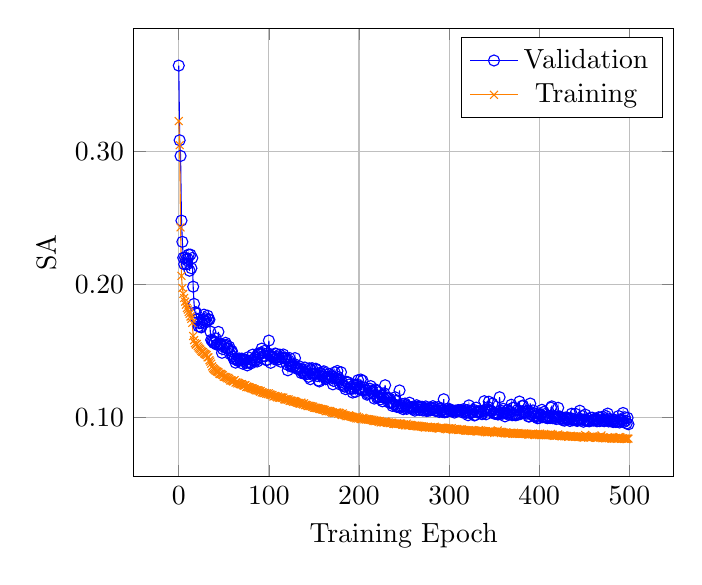
\begin{tikzpicture}
            \begin{axis}[
                    xlabel={Training Epoch},
                    ylabel={SA},
                    grid=major,
                    y tick label style={
                            /pgf/number format/.cd,
                            fixed,
                            fixed zerofill,
                            precision=2,
                            /tikz/.cd
                        },
                    x tick label style={
                            /pgf/number format/.cd,
                            fixed,
                            fixed zerofill,
                            precision=0,
                            /tikz/.cd
                        }
                ]

                \addplot [color=blue, mark=o] coordinates {
                        (0, 0.3642612397670746)
                        (1, 0.30816230177879333)
                        (2, 0.29638269543647766)
                        (3, 0.24779503047466278)
                        (4, 0.23184651136398315)
                        (5, 0.2198907881975174)
                        (6, 0.21503548324108124)
                        (7, 0.2200442999601364)
                        (8, 0.2183714210987091)
                        (9, 0.21492354571819305)
                        (10, 0.21909593045711517)
                        (11, 0.22228820621967316)
                        (12, 0.21013307571411133)
                        (13, 0.2222292423248291)
                        (14, 0.21200594305992126)
                        (15, 0.21970370411872864)
                        (16, 0.1981688141822815)
                        (17, 0.1852240115404129)
                        (18, 0.17863872647285461)
                        (19, 0.17896448075771332)
                        (20, 0.17348074913024902)
                        (21, 0.17394930124282837)
                        (22, 0.1683385819196701)
                        (23, 0.17072145640850067)
                        (24, 0.16794972121715546)
                        (25, 0.16756893694400787)
                        (26, 0.17051784694194794)
                        (27, 0.17318259179592133)
                        (28, 0.17713592946529388)
                        (29, 0.17224742472171783)
                        (30, 0.17441733181476593)
                        (31, 0.17180615663528442)
                        (32, 0.17633609473705292)
                        (33, 0.17372170090675354)
                        (34, 0.17336544394493103)
                        (35, 0.1645120084285736)
                        (36, 0.15820004045963287)
                        (37, 0.15749599039554596)
                        (38, 0.15677249431610107)
                        (39, 0.1557745486497879)
                        (40, 0.15648987889289856)
                        (41, 0.15935319662094116)
                        (42, 0.1546919345855713)
                        (43, 0.1546696573495865)
                        (44, 0.1641864776611328)
                        (45, 0.1547311395406723)
                        (46, 0.15508267283439636)
                        (47, 0.15486635267734528)
                        (48, 0.14847421646118164)
                        (49, 0.15121768414974213)
                        (50, 0.1529177576303482)
                        (51, 0.1540088951587677)
                        (52, 0.15596847236156464)
                        (53, 0.15443311631679535)
                        (54, 0.15168094635009766)
                        (55, 0.151569664478302)
                        (56, 0.15303020179271698)
                        (57, 0.1475178301334381)
                        (58, 0.14982084929943085)
                        (59, 0.14980505406856537)
                        (60, 0.1457129269838333)
                        (61, 0.14396557211875916)
                        (62, 0.1439449042081833)
                        (63, 0.14107736945152283)
                        (64, 0.14395226538181305)
                        (65, 0.14290502667427063)
                        (66, 0.142227903008461)
                        (67, 0.14422062039375305)
                        (68, 0.1431140899658203)
                        (69, 0.14346785843372345)
                        (70, 0.1441183090209961)
                        (71, 0.1402813047170639)
                        (72, 0.14239773154258728)
                        (73, 0.1430475264787674)
                        (74, 0.14328724145889282)
                        (75, 0.14093147218227386)
                        (76, 0.1390315145254135)
                        (77, 0.14516004920005798)
                        (78, 0.140953928232193)
                        (79, 0.14140509068965912)
                        (80, 0.1404506415128708)
                        (81, 0.14305099844932556)
                        (82, 0.1471070647239685)
                        (83, 0.14262378215789795)
                        (84, 0.14188547432422638)
                        (85, 0.14493806660175323)
                        (86, 0.1432170867919922)
                        (87, 0.14192943274974823)
                        (88, 0.14787115156650543)
                        (89, 0.1479308158159256)
                        (90, 0.14819079637527466)
                        (91, 0.1477123200893402)
                        (92, 0.15161770582199097)
                        (93, 0.1482124626636505)
                        (94, 0.14611458778381348)
                        (95, 0.1498469114303589)
                        (96, 0.14587707817554474)
                        (97, 0.14298154413700104)
                        (98, 0.14314737915992737)
                        (99, 0.14813388884067535)
                        (100, 0.15766595304012299)
                        (101, 0.14677797257900238)
                        (102, 0.14094345271587372)
                        (103, 0.14603391289710999)
                        (104, 0.14557534456253052)
                        (105, 0.14489562809467316)
                        (106, 0.14374442398548126)
                        (107, 0.14795255661010742)
                        (108, 0.14764191210269928)
                        (109, 0.14525794982910156)
                        (110, 0.14332744479179382)
                        (111, 0.14371667802333832)
                        (112, 0.1470886468887329)
                        (113, 0.14181427657604218)
                        (114, 0.14512445032596588)
                        (115, 0.14457519352436066)
                        (116, 0.14722731709480286)
                        (117, 0.14420773088932037)
                        (118, 0.14489243924617767)
                        (119, 0.1445659101009369)
                        (120, 0.13966630399227142)
                        (121, 0.13532109558582306)
                        (122, 0.14277306199073792)
                        (123, 0.14452509582042694)
                        (124, 0.13828091323375702)
                        (125, 0.13889558613300323)
                        (126, 0.13970281183719635)
                        (127, 0.13799536228179932)
                        (128, 0.1400895118713379)
                        (129, 0.14450012147426605)
                        (130, 0.13675786554813385)
                        (131, 0.13713456690311432)
                        (132, 0.13691644370555878)
                        (133, 0.13641729950904846)
                        (134, 0.1382821798324585)
                        (135, 0.13649648427963257)
                        (136, 0.13326722383499146)
                        (137, 0.13426950573921204)
                        (138, 0.13533224165439606)
                        (139, 0.13289767503738403)
                        (140, 0.13740451633930206)
                        (141, 0.13221827149391174)
                        (142, 0.13437630236148834)
                        (143, 0.1327919363975525)
                        (144, 0.13043324649333954)
                        (145, 0.13680656254291534)
                        (146, 0.128647118806839)
                        (147, 0.13542695343494415)
                        (148, 0.13690254092216492)
                        (149, 0.13170340657234192)
                        (150, 0.1326272189617157)
                        (151, 0.13315194845199585)
                        (152, 0.13651879131793976)
                        (153, 0.13567855954170227)
                        (154, 0.13096493482589722)
                        (155, 0.12764455378055573)
                        (156, 0.1269553303718567)
                        (157, 0.13354286551475525)
                        (158, 0.13249240815639496)
                        (159, 0.13100364804267883)
                        (160, 0.13387691974639893)
                        (161, 0.13459795713424683)
                        (162, 0.1308733969926834)
                        (163, 0.1286522001028061)
                        (164, 0.12906581163406372)
                        (165, 0.13004672527313232)
                        (166, 0.13050904870033264)
                        (167, 0.1326340138912201)
                        (168, 0.1290406584739685)
                        (169, 0.1308273822069168)
                        (170, 0.13077788054943085)
                        (171, 0.12478146702051163)
                        (172, 0.12729738652706146)
                        (173, 0.13382187485694885)
                        (174, 0.12939012050628662)
                        (175, 0.12910190224647522)
                        (176, 0.1348116099834442)
                        (177, 0.13016657531261444)
                        (178, 0.12830571830272675)
                        (179, 0.12465427815914154)
                        (180, 0.13391080498695374)
                        (181, 0.12645283341407776)
                        (182, 0.12450750172138214)
                        (183, 0.12371997535228729)
                        (184, 0.12301425635814667)
                        (185, 0.12116953730583191)
                        (186, 0.12666092813014984)
                        (187, 0.12655499577522278)
                        (188, 0.12614752352237701)
                        (189, 0.12464017421007156)
                        (190, 0.12165345251560211)
                        (191, 0.12141226977109909)
                        (192, 0.12317687273025513)
                        (193, 0.11857914179563522)
                        (194, 0.12165728211402893)
                        (195, 0.12444253265857697)
                        (196, 0.11914025247097015)
                        (197, 0.12371348589658737)
                        (198, 0.12458214908838272)
                        (199, 0.12793388962745667)
                        (200, 0.12146614491939545)
                        (201, 0.12138141691684723)
                        (202, 0.1283850222826004)
                        (203, 0.12046974897384644)
                        (204, 0.12753723561763763)
                        (205, 0.12042631208896637)
                        (206, 0.12233448028564453)
                        (207, 0.12071352452039719)
                        (208, 0.12015340477228165)
                        (209, 0.11700696498155594)
                        (210, 0.11767660081386566)
                        (211, 0.11834505200386047)
                        (212, 0.12156746536493301)
                        (213, 0.12346906214952469)
                        (214, 0.1189810112118721)
                        (215, 0.11975531280040741)
                        (216, 0.1180712953209877)
                        (217, 0.11406894028186798)
                        (218, 0.12104766815900803)
                        (219, 0.12010745704174042)
                        (220, 0.1144975796341896)
                        (221, 0.11504463106393814)
                        (222, 0.11879950761795044)
                        (223, 0.11540507525205612)
                        (224, 0.11350102722644806)
                        (225, 0.11643911153078079)
                        (226, 0.11201828718185425)
                        (227, 0.11490540206432343)
                        (228, 0.1180834174156189)
                        (229, 0.12411045283079147)
                        (230, 0.11486390978097916)
                        (231, 0.11443126946687698)
                        (232, 0.11485813558101654)
                        (233, 0.11113505065441132)
                        (234, 0.11406294256448746)
                        (235, 0.1108400821685791)
                        (236, 0.11105237901210785)
                        (237, 0.10858374834060669)
                        (238, 0.10983038693666458)
                        (239, 0.1098688393831253)
                        (240, 0.1150963231921196)
                        (241, 0.1122562512755394)
                        (242, 0.10779210180044174)
                        (243, 0.1084485873579979)
                        (244, 0.10772616416215897)
                        (245, 0.12020173668861389)
                        (246, 0.10740221291780472)
                        (247, 0.10853293538093567)
                        (248, 0.11002114415168762)
                        (249, 0.10611610859632492)
                        (250, 0.10729304701089859)
                        (251, 0.11034336686134338)
                        (252, 0.10914287716150284)
                        (253, 0.10634305328130722)
                        (254, 0.10816608369350433)
                        (255, 0.10729016363620758)
                        (256, 0.11101461946964264)
                        (257, 0.10720676928758621)
                        (258, 0.10770659148693085)
                        (259, 0.10670757293701172)
                        (260, 0.1058691218495369)
                        (261, 0.10740391910076141)
                        (262, 0.10502763837575912)
                        (263, 0.10796782374382019)
                        (264, 0.10907702147960663)
                        (265, 0.10798977315425873)
                        (266, 0.10760052502155304)
                        (267, 0.10552917420864105)
                        (268, 0.10739121586084366)
                        (269, 0.10765210539102554)
                        (270, 0.10793623328208923)
                        (271, 0.10507149249315262)
                        (272, 0.10574406385421753)
                        (273, 0.10662934184074402)
                        (274, 0.10817975550889969)
                        (275, 0.10472539812326431)
                        (276, 0.10673657804727554)
                        (277, 0.10501302033662796)
                        (278, 0.10599838942289352)
                        (279, 0.1051982119679451)
                        (280, 0.1071743294596672)
                        (281, 0.10659460723400116)
                        (282, 0.10838329046964645)
                        (283, 0.10649513453245163)
                        (284, 0.10746554285287857)
                        (285, 0.10471688210964203)
                        (286, 0.10549674183130264)
                        (287, 0.10482388734817505)
                        (288, 0.10773033648729324)
                        (289, 0.10399910062551498)
                        (290, 0.10666416585445404)
                        (291, 0.10504450649023056)
                        (292, 0.10538286715745926)
                        (293, 0.10392428189516068)
                        (294, 0.11357368528842926)
                        (295, 0.10373737663030624)
                        (296, 0.1042824536561966)
                        (297, 0.10456965863704681)
                        (298, 0.10420434176921844)
                        (299, 0.10662298649549484)
                        (300, 0.10581599175930023)
                        (301, 0.10539530962705612)
                        (302, 0.10542547702789307)
                        (303, 0.10455667972564697)
                        (304, 0.10510718822479248)
                        (305, 0.10489438474178314)
                        (306, 0.10353948920965195)
                        (307, 0.10503377765417099)
                        (308, 0.10461800545454025)
                        (309, 0.1049058586359024)
                        (310, 0.1054864376783371)
                        (311, 0.1049690917134285)
                        (312, 0.10512875765562057)
                        (313, 0.10540955513715744)
                        (314, 0.10498272627592087)
                        (315, 0.10365733504295349)
                        (316, 0.1061253622174263)
                        (317, 0.10480915009975433)
                        (318, 0.10361495614051819)
                        (319, 0.10330501198768616)
                        (320, 0.10541100800037384)
                        (321, 0.10157286375761032)
                        (322, 0.10897032916545868)
                        (323, 0.10349146276712418)
                        (324, 0.103055439889431)
                        (325, 0.10501162707805634)
                        (326, 0.10406714677810669)
                        (327, 0.1056814193725586)
                        (328, 0.1013910323381424)
                        (329, 0.10174135118722916)
                        (330, 0.10727761685848236)
                        (331, 0.10378766804933548)
                        (332, 0.10393574833869934)
                        (333, 0.1046241819858551)
                        (334, 0.10429513454437256)
                        (335, 0.10407436639070511)
                        (336, 0.10246720910072327)
                        (337, 0.10247030109167099)
                        (338, 0.10420690476894379)
                        (339, 0.11212485283613205)
                        (340, 0.1056864857673645)
                        (341, 0.1022748053073883)
                        (342, 0.10608027875423431)
                        (343, 0.10768669843673706)
                        (344, 0.11174305528402328)
                        (345, 0.10538596659898758)
                        (346, 0.1051575317978859)
                        (347, 0.10458359122276306)
                        (348, 0.11033478379249573)
                        (349, 0.10306604951620102)
                        (350, 0.1034138947725296)
                        (351, 0.10258115828037262)
                        (352, 0.10302148759365082)
                        (353, 0.1028246134519577)
                        (354, 0.1021866425871849)
                        (355, 0.10227540135383606)
                        (356, 0.11509432643651962)
                        (357, 0.10513270646333694)
                        (358, 0.10357730090618134)
                        (359, 0.1026620864868164)
                        (360, 0.10640233010053635)
                        (361, 0.10372718423604965)
                        (362, 0.10070618987083435)
                        (363, 0.10302338749170303)
                        (364, 0.10317865759134293)
                        (365, 0.10559283196926117)
                        (366, 0.10195682942867279)
                        (367, 0.10416223853826523)
                        (368, 0.10378147661685944)
                        (369, 0.10945693403482437)
                        (370, 0.10158827900886536)
                        (371, 0.10725823789834976)
                        (372, 0.10725659132003784)
                        (373, 0.10168609768152237)
                        (374, 0.1015404760837555)
                        (375, 0.10207267850637436)
                        (376, 0.10555356740951538)
                        (377, 0.10214594751596451)
                        (378, 0.11183932423591614)
                        (379, 0.1024467796087265)
                        (380, 0.10335015505552292)
                        (381, 0.108387291431427)
                        (382, 0.10889468342065811)
                        (383, 0.10311893373727798)
                        (384, 0.10419151932001114)
                        (385, 0.10374768823385239)
                        (386, 0.10275396704673767)
                        (387, 0.1050371304154396)
                        (388, 0.10058864206075668)
                        (389, 0.10061877220869064)
                        (390, 0.11036243289709091)
                        (391, 0.10207284986972809)
                        (392, 0.10368669033050537)
                        (393, 0.10519453138113022)
                        (394, 0.10092870146036148)
                        (395, 0.10283329337835312)
                        (396, 0.10059136897325516)
                        (397, 0.10085199028253555)
                        (398, 0.09927231818437576)
                        (399, 0.10295400023460388)
                        (400, 0.09948763251304626)
                        (401, 0.10172662883996964)
                        (402, 0.10179315507411957)
                        (403, 0.10562942177057266)
                        (404, 0.10011424869298935)
                        (405, 0.10403402149677277)
                        (406, 0.10231894254684448)
                        (407, 0.10023051500320435)
                        (408, 0.09959904104471207)
                        (409, 0.09932461380958557)
                        (410, 0.09989305585622787)
                        (411, 0.10102588683366776)
                        (412, 0.09941618889570236)
                        (413, 0.10725805163383484)
                        (414, 0.10822528600692749)
                        (415, 0.09933915734291077)
                        (416, 0.10090713948011398)
                        (417, 0.09923303127288818)
                        (418, 0.1003008708357811)
                        (419, 0.09872575849294662)
                        (420, 0.10062796622514725)
                        (421, 0.1071530282497406)
                        (422, 0.1005990132689476)
                        (423, 0.10057118535041809)
                        (424, 0.09952777624130249)
                        (425, 0.09886609762907028)
                        (426, 0.09786978363990784)
                        (427, 0.09903708845376968)
                        (428, 0.09750035405158997)
                        (429, 0.09986010193824768)
                        (430, 0.09875883907079697)
                        (431, 0.09979492425918579)
                        (432, 0.09879365563392639)
                        (433, 0.09838265180587769)
                        (434, 0.09724664688110352)
                        (435, 0.09933257102966309)
                        (436, 0.10274771600961685)
                        (437, 0.09776882082223892)
                        (438, 0.09875546395778656)
                        (439, 0.09793691337108612)
                        (440, 0.10266563296318054)
                        (441, 0.09778865426778793)
                        (442, 0.09728613495826721)
                        (443, 0.09779971092939377)
                        (444, 0.09845409542322159)
                        (445, 0.1049574539065361)
                        (446, 0.09864106774330139)
                        (447, 0.09837236255407333)
                        (448, 0.10089371353387833)
                        (449, 0.09667672216892242)
                        (450, 0.09767372161149979)
                        (451, 0.10205314308404922)
                        (452, 0.0982363373041153)
                        (453, 0.09740001708269119)
                        (454, 0.0972776785492897)
                        (455, 0.09710512310266495)
                        (456, 0.09707705676555634)
                        (457, 0.09972397983074188)
                        (458, 0.09780332446098328)
                        (459, 0.0997503399848938)
                        (460, 0.09750799834728241)
                        (461, 0.09858956187963486)
                        (462, 0.09782575070858002)
                        (463, 0.09878740459680557)
                        (464, 0.09704836457967758)
                        (465, 0.09730328619480133)
                        (466, 0.10005539655685425)
                        (467, 0.09712009131908417)
                        (468, 0.09965811669826508)
                        (469, 0.09786944836378098)
                        (470, 0.10040489584207535)
                        (471, 0.0974244698882103)
                        (472, 0.09708111733198166)
                        (473, 0.09835208207368851)
                        (474, 0.1009417176246643)
                        (475, 0.09783037006855011)
                        (476, 0.10280980914831161)
                        (477, 0.09690843522548676)
                        (478, 0.09860692918300629)
                        (479, 0.09779246896505356)
                        (480, 0.09696299582719803)
                        (481, 0.09843683987855911)
                        (482, 0.0964645966887474)
                        (483, 0.09706831723451614)
                        (484, 0.0980309322476387)
                        (485, 0.0964948982000351)
                        (486, 0.09678345173597336)
                        (487, 0.09685081988573074)
                        (488, 0.10096345096826553)
                        (489, 0.09612791985273361)
                        (490, 0.09848496317863464)
                        (491, 0.09795217216014862)
                        (492, 0.09728466719388962)
                        (493, 0.10327643901109695)
                        (494, 0.09641874581575394)
                        (495, 0.1000250056385994)
                        (496, 0.09746973216533661)
                        (497, 0.09539739042520523)
                        (498, 0.09964563697576523)
                        (499, 0.09477777779102325)
                    };
                \addlegendentry{Validation}

                \addplot [color=orange, mark=x] coordinates {
                        (0, 0.32259589433670044)
                        (1, 0.3045032024383545)
                        (2, 0.2426912486553192)
                        (3, 0.20629271864891052)
                        (4, 0.1971738636493683)
                        (5, 0.19278647005558014)
                        (6, 0.18960925936698914)
                        (7, 0.18689335882663727)
                        (8, 0.18460871279239655)
                        (9, 0.1821194291114807)
                        (10, 0.18093854188919067)
                        (11, 0.17916400730609894)
                        (12, 0.1777890920639038)
                        (13, 0.17573310434818268)
                        (14, 0.17399895191192627)
                        (15, 0.17098554968833923)
                        (16, 0.16107489168643951)
                        (17, 0.157979354262352)
                        (18, 0.15567870438098907)
                        (19, 0.15464536845684052)
                        (20, 0.15512579679489136)
                        (21, 0.1533866822719574)
                        (22, 0.15244674682617188)
                        (23, 0.15163767337799072)
                        (24, 0.15092633664608002)
                        (25, 0.14995606243610382)
                        (26, 0.14920184016227722)
                        (27, 0.14911425113677979)
                        (28, 0.14804783463478088)
                        (29, 0.1476072520017624)
                        (30, 0.14720579981803894)
                        (31, 0.14662326872348785)
                        (32, 0.14504428207874298)
                        (33, 0.14504405856132507)
                        (34, 0.1429407149553299)
                        (35, 0.1419375240802765)
                        (36, 0.1403297334909439)
                        (37, 0.1382564902305603)
                        (38, 0.13700540363788605)
                        (39, 0.13623175024986267)
                        (40, 0.1356762796640396)
                        (41, 0.1350284069776535)
                        (42, 0.1346394121646881)
                        (43, 0.1342225968837738)
                        (44, 0.13395899534225464)
                        (45, 0.1329270303249359)
                        (46, 0.13245230913162231)
                        (47, 0.13263075053691864)
                        (48, 0.13204969465732574)
                        (49, 0.1315963715314865)
                        (50, 0.13039375841617584)
                        (51, 0.13039274513721466)
                        (52, 0.1303216814994812)
                        (53, 0.12985897064208984)
                        (54, 0.1292581707239151)
                        (55, 0.1296284794807434)
                        (56, 0.1287723183631897)
                        (57, 0.1277025192975998)
                        (58, 0.12780176103115082)
                        (59, 0.12758809328079224)
                        (60, 0.1269274652004242)
                        (61, 0.12716792523860931)
                        (62, 0.12798282504081726)
                        (63, 0.12614555656909943)
                        (64, 0.12629550695419312)
                        (65, 0.1254282295703888)
                        (66, 0.12603135406970978)
                        (67, 0.12549486756324768)
                        (68, 0.12495243549346924)
                        (69, 0.12480489909648895)
                        (70, 0.1249355673789978)
                        (71, 0.12440100312232971)
                        (72, 0.1238408014178276)
                        (73, 0.12383908778429031)
                        (74, 0.12425031512975693)
                        (75, 0.1227283626794815)
                        (76, 0.12316304445266724)
                        (77, 0.12257903814315796)
                        (78, 0.12273576855659485)
                        (79, 0.12236803025007248)
                        (80, 0.12187761068344116)
                        (81, 0.12180956453084946)
                        (82, 0.12171147763729095)
                        (83, 0.1211816594004631)
                        (84, 0.12107442319393158)
                        (85, 0.12050312757492065)
                        (86, 0.12025509029626846)
                        (87, 0.12032884359359741)
                        (88, 0.12024561315774918)
                        (89, 0.12004845589399338)
                        (90, 0.11928636580705643)
                        (91, 0.11984289437532425)
                        (92, 0.1187383234500885)
                        (93, 0.11881618946790695)
                        (94, 0.11820726096630096)
                        (95, 0.11830917000770569)
                        (96, 0.11835069209337234)
                        (97, 0.11769787967205048)
                        (98, 0.11804639548063278)
                        (99, 0.11746221035718918)
                        (100, 0.11803662776947021)
                        (101, 0.1171257272362709)
                        (102, 0.11711136251688004)
                        (103, 0.11658503860235214)
                        (104, 0.11685949563980103)
                        (105, 0.1156092956662178)
                        (106, 0.11595124751329422)
                        (107, 0.11605598777532578)
                        (108, 0.11568287760019302)
                        (109, 0.11504717916250229)
                        (110, 0.11572097986936569)
                        (111, 0.11487729847431183)
                        (112, 0.11463075131177902)
                        (113, 0.11510544270277023)
                        (114, 0.11491890251636505)
                        (115, 0.1146397590637207)
                        (116, 0.11483214050531387)
                        (117, 0.1136140376329422)
                        (118, 0.1133820116519928)
                        (119, 0.11348116397857666)
                        (120, 0.11353923380374908)
                        (121, 0.11314845830202103)
                        (122, 0.11343717575073242)
                        (123, 0.11228705942630768)
                        (124, 0.11267101764678955)
                        (125, 0.11252011358737946)
                        (126, 0.11218297481536865)
                        (127, 0.11159678548574448)
                        (128, 0.11218924820423126)
                        (129, 0.11192233115434647)
                        (130, 0.11161214858293533)
                        (131, 0.11109256744384766)
                        (132, 0.11087636649608612)
                        (133, 0.1108255386352539)
                        (134, 0.1104154959321022)
                        (135, 0.1102522611618042)
                        (136, 0.11107505112886429)
                        (137, 0.11019523441791534)
                        (138, 0.10964047163724899)
                        (139, 0.11050012707710266)
                        (140, 0.10922081023454666)
                        (141, 0.10935060679912567)
                        (142, 0.10904476791620255)
                        (143, 0.1083712950348854)
                        (144, 0.10876040160655975)
                        (145, 0.10854054987430573)
                        (146, 0.10848916321992874)
                        (147, 0.10838639736175537)
                        (148, 0.10791368782520294)
                        (149, 0.10805890709161758)
                        (150, 0.10723981261253357)
                        (151, 0.10723307728767395)
                        (152, 0.10714977979660034)
                        (153, 0.10692116618156433)
                        (154, 0.1069825068116188)
                        (155, 0.10689866542816162)
                        (156, 0.10635554045438766)
                        (157, 0.10613419860601425)
                        (158, 0.10626965761184692)
                        (159, 0.1059078797698021)
                        (160, 0.10585369914770126)
                        (161, 0.10570704191923141)
                        (162, 0.10546375811100006)
                        (163, 0.10458460450172424)
                        (164, 0.10487339645624161)
                        (165, 0.10469433665275574)
                        (166, 0.1049240455031395)
                        (167, 0.10448012501001358)
                        (168, 0.1047101840376854)
                        (169, 0.10411970317363739)
                        (170, 0.10356604307889938)
                        (171, 0.10371676832437515)
                        (172, 0.10314413160085678)
                        (173, 0.10332827270030975)
                        (174, 0.10327046364545822)
                        (175, 0.1036282479763031)
                        (176, 0.10358651727437973)
                        (177, 0.10270463675260544)
                        (178, 0.10343772917985916)
                        (179, 0.10296833515167236)
                        (180, 0.10229818522930145)
                        (181, 0.10173539817333221)
                        (182, 0.10296491533517838)
                        (183, 0.10191889107227325)
                        (184, 0.10160429030656815)
                        (185, 0.1015113964676857)
                        (186, 0.1008361428976059)
                        (187, 0.10104171186685562)
                        (188, 0.10087575018405914)
                        (189, 0.10144879668951035)
                        (190, 0.10084319859743118)
                        (191, 0.10057363659143448)
                        (192, 0.10039404034614563)
                        (193, 0.10040483623743057)
                        (194, 0.09992139041423798)
                        (195, 0.09984247386455536)
                        (196, 0.09993336349725723)
                        (197, 0.09914856404066086)
                        (198, 0.10057901591062546)
                        (199, 0.09910289198160172)
                        (200, 0.0998939573764801)
                        (201, 0.09913869202136993)
                        (202, 0.0986916646361351)
                        (203, 0.09870310872793198)
                        (204, 0.09967135637998581)
                        (205, 0.09926003962755203)
                        (206, 0.09845270216464996)
                        (207, 0.09890557080507278)
                        (208, 0.09832839667797089)
                        (209, 0.0987318903207779)
                        (210, 0.098392553627491)
                        (211, 0.09846632927656174)
                        (212, 0.09823167324066162)
                        (213, 0.09818923473358154)
                        (214, 0.09778589755296707)
                        (215, 0.09828104823827744)
                        (216, 0.09717860072851181)
                        (217, 0.09786196053028107)
                        (218, 0.09712774306535721)
                        (219, 0.09743515402078629)
                        (220, 0.09744451195001602)
                        (221, 0.09706491231918335)
                        (222, 0.0966438353061676)
                        (223, 0.09721661359071732)
                        (224, 0.09608106315135956)
                        (225, 0.09672804176807404)
                        (226, 0.09649999439716339)
                        (227, 0.09616931527853012)
                        (228, 0.09627314656972885)
                        (229, 0.09684353321790695)
                        (230, 0.0965069979429245)
                        (231, 0.09593174606561661)
                        (232, 0.0958542674779892)
                        (233, 0.09619902819395065)
                        (234, 0.09562978893518448)
                        (235, 0.0957062691450119)
                        (236, 0.09594285488128662)
                        (237, 0.09589667618274689)
                        (238, 0.09514041244983673)
                        (239, 0.09505221992731094)
                        (240, 0.09535256028175354)
                        (241, 0.09481523185968399)
                        (242, 0.09566608816385269)
                        (243, 0.09511084854602814)
                        (244, 0.09510792046785355)
                        (245, 0.09502124786376953)
                        (246, 0.09542503952980042)
                        (247, 0.09505966305732727)
                        (248, 0.09439831227064133)
                        (249, 0.09450840204954147)
                        (250, 0.09472893178462982)
                        (251, 0.09400226175785065)
                        (252, 0.09412085264921188)
                        (253, 0.09520948678255081)
                        (254, 0.09385769069194794)
                        (255, 0.0944584384560585)
                        (256, 0.09388864785432816)
                        (257, 0.09422065317630768)
                        (258, 0.09424658119678497)
                        (259, 0.09379631280899048)
                        (260, 0.09362044185400009)
                        (261, 0.09357450902462006)
                        (262, 0.09388591349124908)
                        (263, 0.09347919374704361)
                        (264, 0.09373783320188522)
                        (265, 0.09303667396306992)
                        (266, 0.0937388464808464)
                        (267, 0.09319063276052475)
                        (268, 0.09334122389554977)
                        (269, 0.0930502638220787)
                        (270, 0.0932299792766571)
                        (271, 0.09278278797864914)
                        (272, 0.09301605075597763)
                        (273, 0.09235730767250061)
                        (274, 0.0926043838262558)
                        (275, 0.09277863055467606)
                        (276, 0.09247621893882751)
                        (277, 0.09271536022424698)
                        (278, 0.09228958934545517)
                        (279, 0.09250372648239136)
                        (280, 0.09277592599391937)
                        (281, 0.09208844602108002)
                        (282, 0.09253332763910294)
                        (283, 0.09221075475215912)
                        (284, 0.09292533993721008)
                        (285, 0.09196757525205612)
                        (286, 0.09194757789373398)
                        (287, 0.09198622405529022)
                        (288, 0.09172037988901138)
                        (289, 0.09155353158712387)
                        (290, 0.09184536337852478)
                        (291, 0.0922267958521843)
                        (292, 0.09213751554489136)
                        (293, 0.09214701503515244)
                        (294, 0.09212426841259003)
                        (295, 0.09166939556598663)
                        (296, 0.09109051525592804)
                        (297, 0.09204474091529846)
                        (298, 0.09095022827386856)
                        (299, 0.09158384054899216)
                        (300, 0.09178712218999863)
                        (301, 0.09136615693569183)
                        (302, 0.09128940105438232)
                        (303, 0.09187756478786469)
                        (304, 0.0906350314617157)
                        (305, 0.0911681205034256)
                        (306, 0.09108705818653107)
                        (307, 0.0912785530090332)
                        (308, 0.09080928564071655)
                        (309, 0.09122421592473984)
                        (310, 0.09048647433519363)
                        (311, 0.09061308950185776)
                        (312, 0.09092409908771515)
                        (313, 0.09059736132621765)
                        (314, 0.0910797119140625)
                        (315, 0.09047801792621613)
                        (316, 0.09042001515626907)
                        (317, 0.09046052396297455)
                        (318, 0.08996948599815369)
                        (319, 0.08999159187078476)
                        (320, 0.09010472893714905)
                        (321, 0.08999606966972351)
                        (322, 0.09028758108615875)
                        (323, 0.08991530537605286)
                        (324, 0.0900404155254364)
                        (325, 0.08958743512630463)
                        (326, 0.09034635126590729)
                        (327, 0.09019484370946884)
                        (328, 0.08975132554769516)
                        (329, 0.09004940837621689)
                        (330, 0.0894850641489029)
                        (331, 0.08949929475784302)
                        (332, 0.0894191563129425)
                        (333, 0.09042765945196152)
                        (334, 0.08964452892541885)
                        (335, 0.09015990048646927)
                        (336, 0.08937674760818481)
                        (337, 0.08986972272396088)
                        (338, 0.08955061435699463)
                        (339, 0.08962596952915192)
                        (340, 0.08886126428842545)
                        (341, 0.08960279077291489)
                        (342, 0.0887015163898468)
                        (343, 0.08899430185556412)
                        (344, 0.08894676715135574)
                        (345, 0.0895712822675705)
                        (346, 0.08884891867637634)
                        (347, 0.08937569707632065)
                        (348, 0.08954320102930069)
                        (349, 0.08927956968545914)
                        (350, 0.08822857588529587)
                        (351, 0.08919810503721237)
                        (352, 0.08889438211917877)
                        (353, 0.08855364471673965)
                        (354, 0.09011232852935791)
                        (355, 0.08893435448408127)
                        (356, 0.0887431874871254)
                        (357, 0.0891432911157608)
                        (358, 0.08865148574113846)
                        (359, 0.08905815333127975)
                        (360, 0.08838403224945068)
                        (361, 0.08821317553520203)
                        (362, 0.08805505931377411)
                        (363, 0.08866342902183533)
                        (364, 0.08804836124181747)
                        (365, 0.08802054077386856)
                        (366, 0.08799135684967041)
                        (367, 0.08788738399744034)
                        (368, 0.08836783468723297)
                        (369, 0.08839864283800125)
                        (370, 0.08779532462358475)
                        (371, 0.08772172778844833)
                        (372, 0.08850754052400589)
                        (373, 0.08753075450658798)
                        (374, 0.08805741369724274)
                        (375, 0.08783651888370514)
                        (376, 0.08759810775518417)
                        (377, 0.08829497545957565)
                        (378, 0.08747713267803192)
                        (379, 0.08752515912055969)
                        (380, 0.08777283132076263)
                        (381, 0.08787404745817184)
                        (382, 0.0875975489616394)
                        (383, 0.08788011968135834)
                        (384, 0.08762670308351517)
                        (385, 0.08756037056446075)
                        (386, 0.08754046261310577)
                        (387, 0.08771028369665146)
                        (388, 0.08692952245473862)
                        (389, 0.08727499097585678)
                        (390, 0.08720748126506805)
                        (391, 0.08751031011343002)
                        (392, 0.0872030183672905)
                        (393, 0.08751878887414932)
                        (394, 0.0868971198797226)
                        (395, 0.08672129362821579)
                        (396, 0.08745802938938141)
                        (397, 0.08719099313020706)
                        (398, 0.08691245317459106)
                        (399, 0.08763444423675537)
                        (400, 0.086629718542099)
                        (401, 0.08775145560503006)
                        (402, 0.08660123497247696)
                        (403, 0.08708599209785461)
                        (404, 0.08689682930707932)
                        (405, 0.0866299495100975)
                        (406, 0.08683928847312927)
                        (407, 0.08669567108154297)
                        (408, 0.08656702935695648)
                        (409, 0.08683237433433533)
                        (410, 0.08690844476222992)
                        (411, 0.08667131513357162)
                        (412, 0.0866347998380661)
                        (413, 0.08757057040929794)
                        (414, 0.0864562839269638)
                        (415, 0.0870208740234375)
                        (416, 0.08601780980825424)
                        (417, 0.08604881167411804)
                        (418, 0.086380235850811)
                        (419, 0.08619584888219833)
                        (420, 0.08622798323631287)
                        (421, 0.08716265857219696)
                        (422, 0.08617009967565536)
                        (423, 0.08629803359508514)
                        (424, 0.08592034131288528)
                        (425, 0.08570230007171631)
                        (426, 0.08626176416873932)
                        (427, 0.0863209217786789)
                        (428, 0.08564139157533646)
                        (429, 0.08629448711872101)
                        (430, 0.08565579354763031)
                        (431, 0.08603589236736298)
                        (432, 0.08537989854812622)
                        (433, 0.08567150682210922)
                        (434, 0.0858602523803711)
                        (435, 0.08613691478967667)
                        (436, 0.08557115495204926)
                        (437, 0.08550652116537094)
                        (438, 0.08561351895332336)
                        (439, 0.08577059954404831)
                        (440, 0.08531071245670319)
                        (441, 0.08567821979522705)
                        (442, 0.08554825931787491)
                        (443, 0.08525319397449493)
                        (444, 0.0852651298046112)
                        (445, 0.08551067113876343)
                        (446, 0.08542773127555847)
                        (447, 0.0851091593503952)
                        (448, 0.08515144139528275)
                        (449, 0.08484930545091629)
                        (450, 0.08485221862792969)
                        (451, 0.0866994857788086)
                        (452, 0.08521927148103714)
                        (453, 0.0856841504573822)
                        (454, 0.08477151393890381)
                        (455, 0.08513100445270538)
                        (456, 0.08544640988111496)
                        (457, 0.08481235057115555)
                        (458, 0.08547810465097427)
                        (459, 0.08539856225252151)
                        (460, 0.08569344878196716)
                        (461, 0.08507522195577621)
                        (462, 0.08509450405836105)
                        (463, 0.08465173840522766)
                        (464, 0.08462006598711014)
                        (465, 0.0849723368883133)
                        (466, 0.08526066690683365)
                        (467, 0.08486408740282059)
                        (468, 0.08453112095594406)
                        (469, 0.08640076965093613)
                        (470, 0.08429271727800369)
                        (471, 0.08499062061309814)
                        (472, 0.08475294709205627)
                        (473, 0.08422985672950745)
                        (474, 0.08438841253519058)
                        (475, 0.08436838537454605)
                        (476, 0.08507244288921356)
                        (477, 0.08423476666212082)
                        (478, 0.08477356284856796)
                        (479, 0.08456647396087646)
                        (480, 0.08396923542022705)
                        (481, 0.0842691957950592)
                        (482, 0.08425948768854141)
                        (483, 0.08397545665502548)
                        (484, 0.08422064036130905)
                        (485, 0.08450961858034134)
                        (486, 0.08379387110471725)
                        (487, 0.08416207134723663)
                        (488, 0.08492715656757355)
                        (489, 0.08528566360473633)
                        (490, 0.08500956743955612)
                        (491, 0.08392710238695145)
                        (492, 0.08409436047077179)
                        (493, 0.08426699787378311)
                        (494, 0.08385534584522247)
                        (495, 0.08396556228399277)
                        (496, 0.08385572582483292)
                        (497, 0.08357694745063782)
                        (498, 0.0841343104839325)
                        (499, 0.08396798372268677)
                    };
                \addlegendentry{Training}

            \end{axis}
        \end{tikzpicture}
        \caption{SA over Epochs}
        \label{fig:sa_low_rcgdnae}
    \end{subfigure}
    \hfill
    \begin{subfigure}{0.45\textwidth}
        \centering
        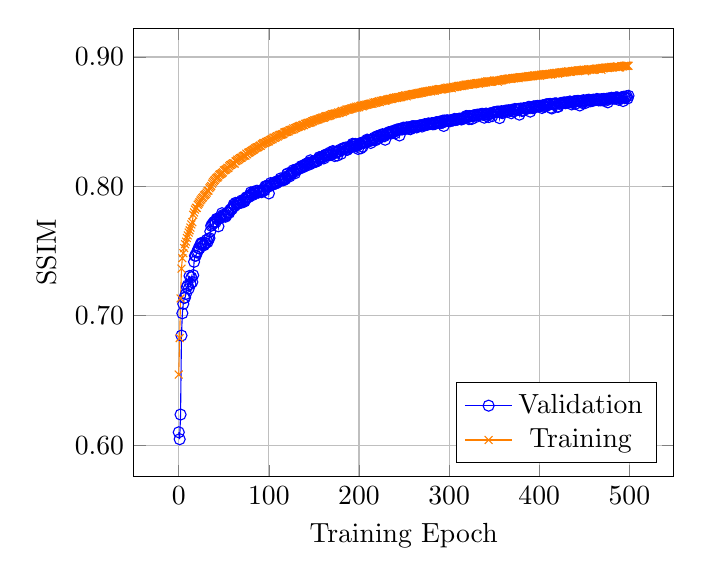
\begin{tikzpicture}
            \begin{axis}[
                    legend pos = south east,
                    xlabel={Training Epoch},
                    ylabel={SSIM},
                    grid=major,
                    y tick label style={
                            /pgf/number format/.cd,
                            fixed,
                            fixed zerofill,
                            precision=2,
                            /tikz/.cd
                        },
                    x tick label style={
                            /pgf/number format/.cd,
                            fixed,
                            fixed zerofill,
                            precision=0,
                            /tikz/.cd
                        }
                ]

                \addplot [color=blue, mark=o] coordinates {
                        (0, 0.6099319458007812)
                        (1, 0.6045882105827332)
                        (2, 0.6236364841461182)
                        (3, 0.6846673488616943)
                        (4, 0.7019184827804565)
                        (5, 0.7092031836509705)
                        (6, 0.713766872882843)
                        (7, 0.7140435576438904)
                        (8, 0.7169386744499207)
                        (9, 0.7222087383270264)
                        (10, 0.723541796207428)
                        (11, 0.7209025621414185)
                        (12, 0.7307871580123901)
                        (13, 0.724607527256012)
                        (14, 0.7296904921531677)
                        (15, 0.726016640663147)
                        (16, 0.7313886880874634)
                        (17, 0.7416901588439941)
                        (18, 0.7463499903678894)
                        (19, 0.7464394569396973)
                        (20, 0.7489717602729797)
                        (21, 0.7499263286590576)
                        (22, 0.7522435188293457)
                        (23, 0.7519903779029846)
                        (24, 0.7550082802772522)
                        (25, 0.7562596797943115)
                        (26, 0.7559720873832703)
                        (27, 0.7544980645179749)
                        (28, 0.7545205950737)
                        (29, 0.7560376524925232)
                        (30, 0.7561415433883667)
                        (31, 0.7586733102798462)
                        (32, 0.7569612264633179)
                        (33, 0.7591782808303833)
                        (34, 0.7600100040435791)
                        (35, 0.7651249170303345)
                        (36, 0.7695897221565247)
                        (37, 0.7704343199729919)
                        (38, 0.7714953422546387)
                        (39, 0.7724166512489319)
                        (40, 0.7728736996650696)
                        (41, 0.7723670601844788)
                        (42, 0.7749536037445068)
                        (43, 0.7747208476066589)
                        (44, 0.7691181898117065)
                        (45, 0.7754834294319153)
                        (46, 0.7756147980690002)
                        (47, 0.7761359214782715)
                        (48, 0.7792536616325378)
                        (49, 0.7779119610786438)
                        (50, 0.7775146961212158)
                        (51, 0.7770771384239197)
                        (52, 0.776581346988678)
                        (53, 0.7776110172271729)
                        (54, 0.7796465158462524)
                        (55, 0.780024528503418)
                        (56, 0.7795938849449158)
                        (57, 0.7817516326904297)
                        (58, 0.7823004722595215)
                        (59, 0.7824553847312927)
                        (60, 0.7839648127555847)
                        (61, 0.7859994173049927)
                        (62, 0.7847976684570312)
                        (63, 0.787270188331604)
                        (64, 0.7866269946098328)
                        (65, 0.786364734172821)
                        (66, 0.7867194414138794)
                        (67, 0.7870317697525024)
                        (68, 0.7872747778892517)
                        (69, 0.7881625294685364)
                        (70, 0.789191722869873)
                        (71, 0.787712812423706)
                        (72, 0.7887452244758606)
                        (73, 0.7883927822113037)
                        (74, 0.7897291779518127)
                        (75, 0.7916038632392883)
                        (76, 0.7915369868278503)
                        (77, 0.7915847301483154)
                        (78, 0.7919408082962036)
                        (79, 0.7934839725494385)
                        (80, 0.7953851222991943)
                        (81, 0.7939786314964294)
                        (82, 0.7932987809181213)
                        (83, 0.7958008050918579)
                        (84, 0.795620322227478)
                        (85, 0.7947326898574829)
                        (86, 0.7965328097343445)
                        (87, 0.7966010570526123)
                        (88, 0.7951325178146362)
                        (89, 0.7959322333335876)
                        (90, 0.7956634759902954)
                        (91, 0.7965239882469177)
                        (92, 0.7955403923988342)
                        (93, 0.7967524528503418)
                        (94, 0.7978553771972656)
                        (95, 0.7968381643295288)
                        (96, 0.8000801205635071)
                        (97, 0.8000231385231018)
                        (98, 0.8005765080451965)
                        (99, 0.8001703023910522)
                        (100, 0.7945590615272522)
                        (101, 0.800179660320282)
                        (102, 0.8025742769241333)
                        (103, 0.8014538884162903)
                        (104, 0.8014906644821167)
                        (105, 0.8018265962600708)
                        (106, 0.8030267357826233)
                        (107, 0.8021632432937622)
                        (108, 0.8023169040679932)
                        (109, 0.8028726577758789)
                        (110, 0.8042731285095215)
                        (111, 0.8042151927947998)
                        (112, 0.8039504885673523)
                        (113, 0.8061922192573547)
                        (114, 0.8050877451896667)
                        (115, 0.8051413297653198)
                        (116, 0.8046735525131226)
                        (117, 0.8064640760421753)
                        (118, 0.805437445640564)
                        (119, 0.8065446019172668)
                        (120, 0.8094179034233093)
                        (121, 0.8100122809410095)
                        (122, 0.8084103465080261)
                        (123, 0.8076874613761902)
                        (124, 0.8090953230857849)
                        (125, 0.8108438849449158)
                        (126, 0.8103029131889343)
                        (127, 0.812508761882782)
                        (128, 0.811207115650177)
                        (129, 0.8101083040237427)
                        (130, 0.8131093382835388)
                        (131, 0.8130581378936768)
                        (132, 0.8135721683502197)
                        (133, 0.8134068250656128)
                        (134, 0.8138489127159119)
                        (135, 0.8144749999046326)
                        (136, 0.8157030344009399)
                        (137, 0.8155339360237122)
                        (138, 0.8148484230041504)
                        (139, 0.8160465359687805)
                        (140, 0.8155829906463623)
                        (141, 0.8171703219413757)
                        (142, 0.8176093101501465)
                        (143, 0.8178655505180359)
                        (144, 0.8183371424674988)
                        (145, 0.8169518113136292)
                        (146, 0.8201456069946289)
                        (147, 0.8187558054924011)
                        (148, 0.8179426193237305)
                        (149, 0.8190796971321106)
                        (150, 0.8191962242126465)
                        (151, 0.8192119002342224)
                        (152, 0.8189831972122192)
                        (153, 0.819913923740387)
                        (154, 0.8197066783905029)
                        (155, 0.821509063243866)
                        (156, 0.822626531124115)
                        (157, 0.8216516971588135)
                        (158, 0.8224295377731323)
                        (159, 0.8228074908256531)
                        (160, 0.8223870992660522)
                        (161, 0.8216291666030884)
                        (162, 0.8239076137542725)
                        (163, 0.8245444297790527)
                        (164, 0.8246860504150391)
                        (165, 0.8241770267486572)
                        (166, 0.8247928023338318)
                        (167, 0.8240742087364197)
                        (168, 0.8262726068496704)
                        (169, 0.8242629766464233)
                        (170, 0.8251757025718689)
                        (171, 0.8273192048072815)
                        (172, 0.8267202973365784)
                        (173, 0.8234665989875793)
                        (174, 0.8261347413063049)
                        (175, 0.8262398838996887)
                        (176, 0.8238444924354553)
                        (177, 0.8267316818237305)
                        (178, 0.8271544575691223)
                        (179, 0.8283925652503967)
                        (180, 0.8251442909240723)
                        (181, 0.8282406330108643)
                        (182, 0.8290841579437256)
                        (183, 0.8296517133712769)
                        (184, 0.8293936252593994)
                        (185, 0.8300108909606934)
                        (186, 0.8281469941139221)
                        (187, 0.8282632827758789)
                        (188, 0.8292558789253235)
                        (189, 0.8299642205238342)
                        (190, 0.8301743865013123)
                        (191, 0.8315134644508362)
                        (192, 0.8307397365570068)
                        (193, 0.8329622149467468)
                        (194, 0.8323505520820618)
                        (195, 0.8307691812515259)
                        (196, 0.8328616619110107)
                        (197, 0.8312768936157227)
                        (198, 0.8315579891204834)
                        (199, 0.8289566040039062)
                        (200, 0.8323734998703003)
                        (201, 0.833146870136261)
                        (202, 0.8294233083724976)
                        (203, 0.8338198065757751)
                        (204, 0.8306493163108826)
                        (205, 0.8339529037475586)
                        (206, 0.8337220549583435)
                        (207, 0.8345279693603516)
                        (208, 0.8344663381576538)
                        (209, 0.836170494556427)
                        (210, 0.8357283473014832)
                        (211, 0.8355547189712524)
                        (212, 0.8349596261978149)
                        (213, 0.8335816860198975)
                        (214, 0.8359658122062683)
                        (215, 0.8359643816947937)
                        (216, 0.8364089727401733)
                        (217, 0.8377293348312378)
                        (218, 0.8355619311332703)
                        (219, 0.8365381360054016)
                        (220, 0.83880615234375)
                        (221, 0.8383975625038147)
                        (222, 0.8373497128486633)
                        (223, 0.8388494253158569)
                        (224, 0.8397984504699707)
                        (225, 0.8384904861450195)
                        (226, 0.840329647064209)
                        (227, 0.840020477771759)
                        (228, 0.8387840390205383)
                        (229, 0.8360903263092041)
                        (230, 0.8402825593948364)
                        (231, 0.8405528664588928)
                        (232, 0.840779185295105)
                        (233, 0.8419482707977295)
                        (234, 0.8412567377090454)
                        (235, 0.8422001600265503)
                        (236, 0.8409761786460876)
                        (237, 0.8417957425117493)
                        (238, 0.8429398536682129)
                        (239, 0.8429275751113892)
                        (240, 0.8409833908081055)
                        (241, 0.8426876664161682)
                        (242, 0.8439932465553284)
                        (243, 0.8436723947525024)
                        (244, 0.8441512584686279)
                        (245, 0.8393691778182983)
                        (246, 0.8445174694061279)
                        (247, 0.8441475033760071)
                        (248, 0.8440172672271729)
                        (249, 0.8453598618507385)
                        (250, 0.8452852964401245)
                        (251, 0.8443237543106079)
                        (252, 0.8447152376174927)
                        (253, 0.8457023501396179)
                        (254, 0.8448356986045837)
                        (255, 0.845538854598999)
                        (256, 0.8444333076477051)
                        (257, 0.844200074672699)
                        (258, 0.8462080359458923)
                        (259, 0.8462980389595032)
                        (260, 0.8465604186058044)
                        (261, 0.8456999659538269)
                        (262, 0.8464930653572083)
                        (263, 0.8462900519371033)
                        (264, 0.8456019759178162)
                        (265, 0.8465883731842041)
                        (266, 0.8464967012405396)
                        (267, 0.8471335172653198)
                        (268, 0.8469797372817993)
                        (269, 0.8472363948822021)
                        (270, 0.8463005423545837)
                        (271, 0.8475216031074524)
                        (272, 0.847155749797821)
                        (273, 0.8481216430664062)
                        (274, 0.8473966121673584)
                        (275, 0.847698986530304)
                        (276, 0.8477429747581482)
                        (277, 0.8487257957458496)
                        (278, 0.8481677174568176)
                        (279, 0.8482771515846252)
                        (280, 0.8483226299285889)
                        (281, 0.8489776253700256)
                        (282, 0.8479785323143005)
                        (283, 0.8487805128097534)
                        (284, 0.8481553196907043)
                        (285, 0.8494026064872742)
                        (286, 0.8495818376541138)
                        (287, 0.8494705557823181)
                        (288, 0.8492586612701416)
                        (289, 0.8499434590339661)
                        (290, 0.8491243720054626)
                        (291, 0.8502105474472046)
                        (292, 0.8490667343139648)
                        (293, 0.8508419394493103)
                        (294, 0.8467293977737427)
                        (295, 0.8509299755096436)
                        (296, 0.8505046367645264)
                        (297, 0.850904643535614)
                        (298, 0.8510826826095581)
                        (299, 0.850524365901947)
                        (300, 0.8509116768836975)
                        (301, 0.8503379821777344)
                        (302, 0.8509927988052368)
                        (303, 0.8513217568397522)
                        (304, 0.8508756160736084)
                        (305, 0.8513988852500916)
                        (306, 0.8521711230278015)
                        (307, 0.8513607382774353)
                        (308, 0.8518812656402588)
                        (309, 0.851594865322113)
                        (310, 0.8519449830055237)
                        (311, 0.8523080945014954)
                        (312, 0.8523196578025818)
                        (313, 0.8519379496574402)
                        (314, 0.8517886996269226)
                        (315, 0.8527776598930359)
                        (316, 0.8524304032325745)
                        (317, 0.852996289730072)
                        (318, 0.8529236912727356)
                        (319, 0.8544480204582214)
                        (320, 0.8532332181930542)
                        (321, 0.8543362021446228)
                        (322, 0.8520147800445557)
                        (323, 0.8543866276741028)
                        (324, 0.8542383909225464)
                        (325, 0.8521021008491516)
                        (326, 0.8545191287994385)
                        (327, 0.8547500371932983)
                        (328, 0.8549565076828003)
                        (329, 0.8551082015037537)
                        (330, 0.8537251949310303)
                        (331, 0.8553948402404785)
                        (332, 0.855376124382019)
                        (333, 0.8553593158721924)
                        (334, 0.8553045988082886)
                        (335, 0.8556684255599976)
                        (336, 0.8560576438903809)
                        (337, 0.8560610413551331)
                        (338, 0.8552807569503784)
                        (339, 0.8531149625778198)
                        (340, 0.8555136919021606)
                        (341, 0.8563070893287659)
                        (342, 0.8556404113769531)
                        (343, 0.855340838432312)
                        (344, 0.8535860776901245)
                        (345, 0.8563786745071411)
                        (346, 0.8562180995941162)
                        (347, 0.8565056920051575)
                        (348, 0.8543700575828552)
                        (349, 0.8571778535842896)
                        (350, 0.8572281002998352)
                        (351, 0.8572161197662354)
                        (352, 0.8575297594070435)
                        (353, 0.8577700257301331)
                        (354, 0.8576115965843201)
                        (355, 0.857807993888855)
                        (356, 0.8527935743331909)
                        (357, 0.8573569059371948)
                        (358, 0.858135461807251)
                        (359, 0.8566341996192932)
                        (360, 0.8571526408195496)
                        (361, 0.8582282066345215)
                        (362, 0.8584581613540649)
                        (363, 0.8584153652191162)
                        (364, 0.858657717704773)
                        (365, 0.8575711846351624)
                        (366, 0.8588408827781677)
                        (367, 0.8585392236709595)
                        (368, 0.8586889505386353)
                        (369, 0.8565617203712463)
                        (370, 0.8592931628227234)
                        (371, 0.8578522801399231)
                        (372, 0.858097493648529)
                        (373, 0.8599067330360413)
                        (374, 0.8595935106277466)
                        (375, 0.859437882900238)
                        (376, 0.8590569496154785)
                        (377, 0.859898567199707)
                        (378, 0.8554719686508179)
                        (379, 0.8600776791572571)
                        (380, 0.8601167798042297)
                        (381, 0.8582636713981628)
                        (382, 0.8586201667785645)
                        (383, 0.8605546355247498)
                        (384, 0.8600375652313232)
                        (385, 0.8600285053253174)
                        (386, 0.8605150580406189)
                        (387, 0.8601354360580444)
                        (388, 0.8614178895950317)
                        (389, 0.8614698052406311)
                        (390, 0.8578036427497864)
                        (391, 0.8611426949501038)
                        (392, 0.861009955406189)
                        (393, 0.8603866100311279)
                        (394, 0.8619409203529358)
                        (395, 0.8610011339187622)
                        (396, 0.8618767261505127)
                        (397, 0.8619390726089478)
                        (398, 0.8622551560401917)
                        (399, 0.8618860840797424)
                        (400, 0.8622137308120728)
                        (401, 0.8620991110801697)
                        (402, 0.8623150587081909)
                        (403, 0.8606099486351013)
                        (404, 0.8626759052276611)
                        (405, 0.8613936305046082)
                        (406, 0.8620977401733398)
                        (407, 0.8632007241249084)
                        (408, 0.8634211421012878)
                        (409, 0.8630929589271545)
                        (410, 0.8635743856430054)
                        (411, 0.8630906343460083)
                        (412, 0.8637908697128296)
                        (413, 0.8608751893043518)
                        (414, 0.8602356314659119)
                        (415, 0.8637567758560181)
                        (416, 0.8635281920433044)
                        (417, 0.864083468914032)
                        (418, 0.8640505075454712)
                        (419, 0.8641428351402283)
                        (420, 0.8616181015968323)
                        (421, 0.8615262508392334)
                        (422, 0.863908052444458)
                        (423, 0.8639376163482666)
                        (424, 0.8644313216209412)
                        (425, 0.8645175695419312)
                        (426, 0.8645179867744446)
                        (427, 0.864753007888794)
                        (428, 0.8649231195449829)
                        (429, 0.8642891645431519)
                        (430, 0.8649073839187622)
                        (431, 0.8648029565811157)
                        (432, 0.864935576915741)
                        (433, 0.8650332689285278)
                        (434, 0.8656614422798157)
                        (435, 0.8650004267692566)
                        (436, 0.8633812665939331)
                        (437, 0.8649258017539978)
                        (438, 0.8654884696006775)
                        (439, 0.8658264875411987)
                        (440, 0.8637858629226685)
                        (441, 0.8659267425537109)
                        (442, 0.8660051822662354)
                        (443, 0.8660919666290283)
                        (444, 0.8659945726394653)
                        (445, 0.8625652194023132)
                        (446, 0.8659201264381409)
                        (447, 0.8660379648208618)
                        (448, 0.8644769787788391)
                        (449, 0.866666316986084)
                        (450, 0.8659176826477051)
                        (451, 0.8643945455551147)
                        (452, 0.866090714931488)
                        (453, 0.8667821288108826)
                        (454, 0.8668058514595032)
                        (455, 0.8670117259025574)
                        (456, 0.866701602935791)
                        (457, 0.86577969789505)
                        (458, 0.8667163848876953)
                        (459, 0.8660731911659241)
                        (460, 0.8670812249183655)
                        (461, 0.8666978478431702)
                        (462, 0.8667587041854858)
                        (463, 0.8668264150619507)
                        (464, 0.8676198124885559)
                        (465, 0.867201030254364)
                        (466, 0.866495668888092)
                        (467, 0.8671318292617798)
                        (468, 0.8665593266487122)
                        (469, 0.8674129843711853)
                        (470, 0.8665297031402588)
                        (471, 0.8675543665885925)
                        (472, 0.8676292896270752)
                        (473, 0.8672685623168945)
                        (474, 0.8663263916969299)
                        (475, 0.8677735924720764)
                        (476, 0.8649720549583435)
                        (477, 0.8679994344711304)
                        (478, 0.8676636219024658)
                        (479, 0.8680641651153564)
                        (480, 0.8685001730918884)
                        (481, 0.8679130673408508)
                        (482, 0.8684011697769165)
                        (483, 0.8678070306777954)
                        (484, 0.8682539463043213)
                        (485, 0.8687377572059631)
                        (486, 0.8687553405761719)
                        (487, 0.8687092661857605)
                        (488, 0.8669506311416626)
                        (489, 0.8682715892791748)
                        (490, 0.8682588934898376)
                        (491, 0.8685242533683777)
                        (492, 0.8690784573554993)
                        (493, 0.8659768104553223)
                        (494, 0.8693612813949585)
                        (495, 0.8682109713554382)
                        (496, 0.8689757585525513)
                        (497, 0.8697605133056641)
                        (498, 0.8679488301277161)
                        (499, 0.8700544834136963)
                    };
                \addlegendentry{Validation}

                \addplot [color=orange, mark=x] coordinates {
                        (0, 0.6545559167861938)
                        (1, 0.682753324508667)
                        (2, 0.7133713364601135)
                        (3, 0.7364510297775269)
                        (4, 0.7445240616798401)
                        (5, 0.7483895421028137)
                        (6, 0.7522908449172974)
                        (7, 0.7553314566612244)
                        (8, 0.7572795152664185)
                        (9, 0.7601293921470642)
                        (10, 0.7621873021125793)
                        (11, 0.7643293142318726)
                        (12, 0.7660314440727234)
                        (13, 0.7682055234909058)
                        (14, 0.7705977559089661)
                        (15, 0.772331953048706)
                        (16, 0.7780157327651978)
                        (17, 0.7798338532447815)
                        (18, 0.7821124792098999)
                        (19, 0.7835333943367004)
                        (20, 0.7833361625671387)
                        (21, 0.7857378721237183)
                        (22, 0.7867106795310974)
                        (23, 0.7877488136291504)
                        (24, 0.789100706577301)
                        (25, 0.789871871471405)
                        (26, 0.7909687161445618)
                        (27, 0.7915932536125183)
                        (28, 0.7929434180259705)
                        (29, 0.7935027480125427)
                        (30, 0.794182300567627)
                        (31, 0.7952650785446167)
                        (32, 0.7965852618217468)
                        (33, 0.7967120409011841)
                        (34, 0.7986055016517639)
                        (35, 0.79940265417099)
                        (36, 0.8003368973731995)
                        (37, 0.8020787239074707)
                        (38, 0.8032847046852112)
                        (39, 0.8043220639228821)
                        (40, 0.805005669593811)
                        (41, 0.8059808611869812)
                        (42, 0.8066454529762268)
                        (43, 0.8069318532943726)
                        (44, 0.8076846599578857)
                        (45, 0.8088636994361877)
                        (46, 0.809319257736206)
                        (47, 0.8097274899482727)
                        (48, 0.8103033304214478)
                        (49, 0.8108689188957214)
                        (50, 0.8123657703399658)
                        (51, 0.812553346157074)
                        (52, 0.8129841089248657)
                        (53, 0.8135504126548767)
                        (54, 0.8144349455833435)
                        (55, 0.8141757249832153)
                        (56, 0.8155243396759033)
                        (57, 0.8163958191871643)
                        (58, 0.8166863918304443)
                        (59, 0.8172754049301147)
                        (60, 0.8178781270980835)
                        (61, 0.8177937865257263)
                        (62, 0.8176663517951965)
                        (63, 0.8193897008895874)
                        (64, 0.8196820616722107)
                        (65, 0.8206510543823242)
                        (66, 0.8203775882720947)
                        (67, 0.821128249168396)
                        (68, 0.8217647671699524)
                        (69, 0.8221642971038818)
                        (70, 0.8223001956939697)
                        (71, 0.8231655359268188)
                        (72, 0.8236342072486877)
                        (73, 0.823927104473114)
                        (74, 0.8237666487693787)
                        (75, 0.8252802491188049)
                        (76, 0.824824333190918)
                        (77, 0.8260168433189392)
                        (78, 0.8261917233467102)
                        (79, 0.8265417218208313)
                        (80, 0.8271276950836182)
                        (81, 0.8275653123855591)
                        (82, 0.8281065821647644)
                        (83, 0.8284007906913757)
                        (84, 0.828893780708313)
                        (85, 0.8295623064041138)
                        (86, 0.8299152851104736)
                        (87, 0.8301784992218018)
                        (88, 0.8303728699684143)
                        (89, 0.8309303522109985)
                        (90, 0.8315881490707397)
                        (91, 0.8313755393028259)
                        (92, 0.8324516415596008)
                        (93, 0.8328410983085632)
                        (94, 0.8335369825363159)
                        (95, 0.833577573299408)
                        (96, 0.8336036801338196)
                        (97, 0.8343566656112671)
                        (98, 0.8344268202781677)
                        (99, 0.8349305987358093)
                        (100, 0.8348406553268433)
                        (101, 0.8357781767845154)
                        (102, 0.8359789252281189)
                        (103, 0.836624801158905)
                        (104, 0.8364390134811401)
                        (105, 0.8376113176345825)
                        (106, 0.8376826643943787)
                        (107, 0.837567925453186)
                        (108, 0.838248074054718)
                        (109, 0.8388890624046326)
                        (110, 0.8386052846908569)
                        (111, 0.8393670916557312)
                        (112, 0.8399277925491333)
                        (113, 0.8398308157920837)
                        (114, 0.8400006294250488)
                        (115, 0.8404009342193604)
                        (116, 0.8404697775840759)
                        (117, 0.8416072130203247)
                        (118, 0.8418372273445129)
                        (119, 0.8420983552932739)
                        (120, 0.842228353023529)
                        (121, 0.8425588011741638)
                        (122, 0.8425516486167908)
                        (123, 0.8435143828392029)
                        (124, 0.8434950709342957)
                        (125, 0.8438518643379211)
                        (126, 0.8438557982444763)
                        (127, 0.8448304533958435)
                        (128, 0.8442585468292236)
                        (129, 0.8450623154640198)
                        (130, 0.8452973365783691)
                        (131, 0.8457186818122864)
                        (132, 0.8459537625312805)
                        (133, 0.8462072610855103)
                        (134, 0.8466621041297913)
                        (135, 0.8468790650367737)
                        (136, 0.8464324474334717)
                        (137, 0.8472861051559448)
                        (138, 0.8476558327674866)
                        (139, 0.847339391708374)
                        (140, 0.848386824131012)
                        (141, 0.848359227180481)
                        (142, 0.8486677408218384)
                        (143, 0.8492464423179626)
                        (144, 0.849056601524353)
                        (145, 0.8491858839988708)
                        (146, 0.8495408892631531)
                        (147, 0.8495908975601196)
                        (148, 0.8502975702285767)
                        (149, 0.8503420352935791)
                        (150, 0.8510292172431946)
                        (151, 0.8509935140609741)
                        (152, 0.8512575626373291)
                        (153, 0.8516293168067932)
                        (154, 0.8516667485237122)
                        (155, 0.8518167734146118)
                        (156, 0.8522501587867737)
                        (157, 0.8525874614715576)
                        (158, 0.8527052402496338)
                        (159, 0.8530715703964233)
                        (160, 0.8531444072723389)
                        (161, 0.8530973196029663)
                        (162, 0.853649377822876)
                        (163, 0.8543274998664856)
                        (164, 0.8542059063911438)
                        (165, 0.8544942736625671)
                        (166, 0.8542600870132446)
                        (167, 0.8546711802482605)
                        (168, 0.8549761176109314)
                        (169, 0.8552484512329102)
                        (170, 0.8559186458587646)
                        (171, 0.8558093905448914)
                        (172, 0.856112539768219)
                        (173, 0.8562015295028687)
                        (174, 0.8563633561134338)
                        (175, 0.8562495708465576)
                        (176, 0.8565227389335632)
                        (177, 0.8571740388870239)
                        (178, 0.8566976189613342)
                        (179, 0.8571083545684814)
                        (180, 0.85762619972229)
                        (181, 0.8583359718322754)
                        (182, 0.8574396967887878)
                        (183, 0.8581953644752502)
                        (184, 0.858513593673706)
                        (185, 0.8587677478790283)
                        (186, 0.8593847155570984)
                        (187, 0.859318196773529)
                        (188, 0.8594056963920593)
                        (189, 0.8594691157341003)
                        (190, 0.8597106337547302)
                        (191, 0.860145628452301)
                        (192, 0.8602884411811829)
                        (193, 0.860383152961731)
                        (194, 0.8607974648475647)
                        (195, 0.8609701991081238)
                        (196, 0.8609036803245544)
                        (197, 0.8615879416465759)
                        (198, 0.8609615564346313)
                        (199, 0.8617550134658813)
                        (200, 0.8612180948257446)
                        (201, 0.8620014786720276)
                        (202, 0.8623936772346497)
                        (203, 0.8624963760375977)
                        (204, 0.8618197441101074)
                        (205, 0.8623381853103638)
                        (206, 0.8630220293998718)
                        (207, 0.8627303242683411)
                        (208, 0.8632199764251709)
                        (209, 0.8631473779678345)
                        (210, 0.8634454607963562)
                        (211, 0.8636202812194824)
                        (212, 0.8638826012611389)
                        (213, 0.863807737827301)
                        (214, 0.8641439080238342)
                        (215, 0.8638460040092468)
                        (216, 0.8648000955581665)
                        (217, 0.8643954396247864)
                        (218, 0.8649800419807434)
                        (219, 0.8646860718727112)
                        (220, 0.865094780921936)
                        (221, 0.8653123378753662)
                        (222, 0.8658092617988586)
                        (223, 0.8652772903442383)
                        (224, 0.8661778569221497)
                        (225, 0.8658698201179504)
                        (226, 0.8661766052246094)
                        (227, 0.8664609789848328)
                        (228, 0.8665944933891296)
                        (229, 0.8663181662559509)
                        (230, 0.8665010929107666)
                        (231, 0.8670344352722168)
                        (232, 0.8672536015510559)
                        (233, 0.8672563433647156)
                        (234, 0.8676610589027405)
                        (235, 0.8676436543464661)
                        (236, 0.8675834536552429)
                        (237, 0.8677579760551453)
                        (238, 0.8682795763015747)
                        (239, 0.8684498071670532)
                        (240, 0.8682470321655273)
                        (241, 0.8687707781791687)
                        (242, 0.868403434753418)
                        (243, 0.8689063787460327)
                        (244, 0.8688737154006958)
                        (245, 0.8691047430038452)
                        (246, 0.8689329624176025)
                        (247, 0.8692337274551392)
                        (248, 0.8697262406349182)
                        (249, 0.8697540163993835)
                        (250, 0.869698166847229)
                        (251, 0.8703205585479736)
                        (252, 0.8701855540275574)
                        (253, 0.8696426749229431)
                        (254, 0.8706443905830383)
                        (255, 0.8704321980476379)
                        (256, 0.8708058595657349)
                        (257, 0.8707339763641357)
                        (258, 0.8708789944648743)
                        (259, 0.8712529540061951)
                        (260, 0.8714008927345276)
                        (261, 0.8713799118995667)
                        (262, 0.8714248538017273)
                        (263, 0.8717495203018188)
                        (264, 0.8716808557510376)
                        (265, 0.8721425533294678)
                        (266, 0.8718351721763611)
                        (267, 0.8723664283752441)
                        (268, 0.8722644448280334)
                        (269, 0.872446596622467)
                        (270, 0.8724706172943115)
                        (271, 0.8729493021965027)
                        (272, 0.8728635907173157)
                        (273, 0.8732865452766418)
                        (274, 0.8733120560646057)
                        (275, 0.8732732534408569)
                        (276, 0.8735525012016296)
                        (277, 0.8733871579170227)
                        (278, 0.873863160610199)
                        (279, 0.873921275138855)
                        (280, 0.8734474182128906)
                        (281, 0.8742730021476746)
                        (282, 0.874009907245636)
                        (283, 0.8744150400161743)
                        (284, 0.8739685416221619)
                        (285, 0.8747214078903198)
                        (286, 0.8748422265052795)
                        (287, 0.8745852708816528)
                        (288, 0.8750486969947815)
                        (289, 0.8752331137657166)
                        (290, 0.875194251537323)
                        (291, 0.8749718070030212)
                        (292, 0.8750409483909607)
                        (293, 0.8752520680427551)
                        (294, 0.8753492832183838)
                        (295, 0.8755921721458435)
                        (296, 0.8761051297187805)
                        (297, 0.8755752444267273)
                        (298, 0.8764017820358276)
                        (299, 0.8760553598403931)
                        (300, 0.8760563731193542)
                        (301, 0.8763459920883179)
                        (302, 0.876422643661499)
                        (303, 0.8759070038795471)
                        (304, 0.8770017027854919)
                        (305, 0.8767836689949036)
                        (306, 0.8768594264984131)
                        (307, 0.8768519163131714)
                        (308, 0.8772048950195312)
                        (309, 0.8770559430122375)
                        (310, 0.8776037693023682)
                        (311, 0.8776655197143555)
                        (312, 0.877536952495575)
                        (313, 0.877825140953064)
                        (314, 0.8774977922439575)
                        (315, 0.8780120611190796)
                        (316, 0.8781573176383972)
                        (317, 0.8780158162117004)
                        (318, 0.8785540461540222)
                        (319, 0.8786953687667847)
                        (320, 0.8785520792007446)
                        (321, 0.8786740899085999)
                        (322, 0.8786131143569946)
                        (323, 0.8789741396903992)
                        (324, 0.8790256381034851)
                        (325, 0.8793192505836487)
                        (326, 0.878841757774353)
                        (327, 0.8791705369949341)
                        (328, 0.8794801235198975)
                        (329, 0.8792915344238281)
                        (330, 0.879751980304718)
                        (331, 0.87984299659729)
                        (332, 0.8799341917037964)
                        (333, 0.879336416721344)
                        (334, 0.8800802826881409)
                        (335, 0.8797495365142822)
                        (336, 0.8802894949913025)
                        (337, 0.88004070520401)
                        (338, 0.8803482055664062)
                        (339, 0.8801413178443909)
                        (340, 0.8809307217597961)
                        (341, 0.8804313540458679)
                        (342, 0.8811662197113037)
                        (343, 0.8810166716575623)
                        (344, 0.8810644745826721)
                        (345, 0.8808539509773254)
                        (346, 0.8813155889511108)
                        (347, 0.8809006810188293)
                        (348, 0.8811235427856445)
                        (349, 0.8814059495925903)
                        (350, 0.8819133639335632)
                        (351, 0.8815072178840637)
                        (352, 0.8817476630210876)
                        (353, 0.881867527961731)
                        (354, 0.8809473514556885)
                        (355, 0.8818473815917969)
                        (356, 0.8819355368614197)
                        (357, 0.8819015622138977)
                        (358, 0.8823456168174744)
                        (359, 0.8820170760154724)
                        (360, 0.8825230598449707)
                        (361, 0.8827179074287415)
                        (362, 0.8829228281974792)
                        (363, 0.8826255202293396)
                        (364, 0.8830176591873169)
                        (365, 0.883108913898468)
                        (366, 0.8832457065582275)
                        (367, 0.8833937644958496)
                        (368, 0.8831712007522583)
                        (369, 0.8831747770309448)
                        (370, 0.8836037516593933)
                        (371, 0.8837499022483826)
                        (372, 0.8834567666053772)
                        (373, 0.8839051127433777)
                        (374, 0.8837518692016602)
                        (375, 0.8839712738990784)
                        (376, 0.8841108679771423)
                        (377, 0.8836439251899719)
                        (378, 0.8843765258789062)
                        (379, 0.8844701647758484)
                        (380, 0.8843252658843994)
                        (381, 0.8843629360198975)
                        (382, 0.8844315409660339)
                        (383, 0.8844712376594543)
                        (384, 0.8846207857131958)
                        (385, 0.88480144739151)
                        (386, 0.8847886323928833)
                        (387, 0.8847818374633789)
                        (388, 0.8853177428245544)
                        (389, 0.8850796818733215)
                        (390, 0.8852546811103821)
                        (391, 0.8851083517074585)
                        (392, 0.8853664994239807)
                        (393, 0.8852691650390625)
                        (394, 0.8857526779174805)
                        (395, 0.8858221769332886)
                        (396, 0.8855368494987488)
                        (397, 0.8856944441795349)
                        (398, 0.8859434723854065)
                        (399, 0.8855106234550476)
                        (400, 0.8862487077713013)
                        (401, 0.8854668140411377)
                        (402, 0.8863965272903442)
                        (403, 0.8861554861068726)
                        (404, 0.8863897323608398)
                        (405, 0.8865447640419006)
                        (406, 0.8865132331848145)
                        (407, 0.8867226839065552)
                        (408, 0.8868284821510315)
                        (409, 0.8866733312606812)
                        (410, 0.8864932656288147)
                        (411, 0.8869091272354126)
                        (412, 0.8869791030883789)
                        (413, 0.8865270614624023)
                        (414, 0.8872684836387634)
                        (415, 0.886834442615509)
                        (416, 0.8876302242279053)
                        (417, 0.8874908089637756)
                        (418, 0.8872953653335571)
                        (419, 0.887706458568573)
                        (420, 0.8876751661300659)
                        (421, 0.8871347308158875)
                        (422, 0.8879243731498718)
                        (423, 0.8878830671310425)
                        (424, 0.8880655765533447)
                        (425, 0.8882772922515869)
                        (426, 0.8879584670066833)
                        (427, 0.888093113899231)
                        (428, 0.8884660005569458)
                        (429, 0.8880902528762817)
                        (430, 0.8886049389839172)
                        (431, 0.8884268999099731)
                        (432, 0.8889918923377991)
                        (433, 0.8887317776679993)
                        (434, 0.8885903358459473)
                        (435, 0.888568103313446)
                        (436, 0.8890379667282104)
                        (437, 0.8891679048538208)
                        (438, 0.8889802694320679)
                        (439, 0.8891645669937134)
                        (440, 0.8893902897834778)
                        (441, 0.88911372423172)
                        (442, 0.8893924355506897)
                        (443, 0.8897018432617188)
                        (444, 0.8896532654762268)
                        (445, 0.8896397352218628)
                        (446, 0.8896615505218506)
                        (447, 0.8899214267730713)
                        (448, 0.8897684216499329)
                        (449, 0.8902068734169006)
                        (450, 0.8901857733726501)
                        (451, 0.8890545964241028)
                        (452, 0.8901728391647339)
                        (453, 0.8897610306739807)
                        (454, 0.8904637098312378)
                        (455, 0.890453040599823)
                        (456, 0.8901263475418091)
                        (457, 0.890676736831665)
                        (458, 0.8902300000190735)
                        (459, 0.8904345631599426)
                        (460, 0.8899683356285095)
                        (461, 0.8906669020652771)
                        (462, 0.8906479477882385)
                        (463, 0.8910255432128906)
                        (464, 0.8909855484962463)
                        (465, 0.8908961415290833)
                        (466, 0.8907960057258606)
                        (467, 0.8911300301551819)
                        (468, 0.8914044499397278)
                        (469, 0.890094518661499)
                        (470, 0.8916628360748291)
                        (471, 0.8913111090660095)
                        (472, 0.8914328217506409)
                        (473, 0.89179527759552)
                        (474, 0.8917948007583618)
                        (475, 0.89173424243927)
                        (476, 0.8915325403213501)
                        (477, 0.8920408487319946)
                        (478, 0.8917842507362366)
                        (479, 0.8919591903686523)
                        (480, 0.8923810124397278)
                        (481, 0.8922325372695923)
                        (482, 0.8922450542449951)
                        (483, 0.8924264907836914)
                        (484, 0.8923484683036804)
                        (485, 0.8922988772392273)
                        (486, 0.8927558660507202)
                        (487, 0.892606258392334)
                        (488, 0.8920719623565674)
                        (489, 0.8918409943580627)
                        (490, 0.8921775221824646)
                        (491, 0.8929856419563293)
                        (492, 0.8928956985473633)
                        (493, 0.8927544355392456)
                        (494, 0.8931478261947632)
                        (495, 0.8931061029434204)
                        (496, 0.8932587504386902)
                        (497, 0.8933975696563721)
                        (498, 0.8931828141212463)
                        (499, 0.8932528495788574)
                    };
                \addlegendentry{Training}

            \end{axis}
        \end{tikzpicture}
        \caption{SSIM over Epochs}
        \label{fig:ssim_low_rcgdnae}
    \end{subfigure}
    \caption{Training and Validation Metrics over Epochs for RCGDNAE low bitrate Model}
    \label{fig:training_metrics_rcgdnae_low}

\end{figure}

The training and validation metrics lack the usual plateau patterns often seen in overfitting scenarios.
This suggests that the model is still learning and has not yet reached their optimal performance.
This is a positive indication that the model has the potential for further improvement with continued training.
However, it wasn't possible to explore longer training due to computational resource constraints.

\section{Summary}
The RCGDNAE model demonstrates effective training behavior, as evidenced by the consistent improvement in loss and evaluation metrics over the training epochs.
The model itself is quite simple computationally, with a modest number of parameters and a straightforward architecture.
The RCGDNAE model was implemented with 4 main components: the encoder, decoder, hyperprior network, and context model.
The encoder and decoder both consist of a series of convolutional layers followed by GDN or inverse GDN layers.
The hyperprior network consists of convolutional layers that process the latent representation to produce the parameters for the distribution modeling.
The context model also consists of convolutional layers that process the latent representation in a sequential manner.
The overall architecture of the model is designed to efficiently compress hyperspectral images while maintaining high reconstruction quality.



\chapter{Small Segmentation model}\label{chap:small_segmenter}
In addition to the aforementioned compression models, a small segmentation model was also implemented as part of this thesis work.
The segmentation model is designed specifically for memory-efficient per-pixel classification of hyperspectral data, requiring approximately 1--2 GB of VRAM for a batch size of 1.

\section{Model architecture}
The small\_segmenter takes 5D input tensors of shape $(B, H, W, D, 1)$ where $B$ is the batch size, $H \times W$ is the spatial resolution (128$\times$128), and $D$ is the number of spectral bands (202 for HySpecNet).
The model outputs 2D spatial segmentation masks of shape $(B, H, W, C)$ where $C$ is the number of classes.

Unlike traditional segmentation architectures such as U-Net ~\cite{ronneberger2015u} that use spatial downsampling and upsampling with skip connections, this model employs a progressive spectral reduction strategy that preserves full spatial resolution throughout the network.
This design choice is motivated by the nature of hyperspectral segmentation, where maintaining spatial detail is critical for accurate per-pixel classification.
The designed Small Segmentation architecture is presented in Figure~\ref{fig:small_segmenter_architecture}.

\section{Model implementation}
The model uses a series of 3D convolutions to ensure both spatial and spectral features are utilized.
Next, the architecture collapses the spectral dimension using a $1 \times 1 \times 1$ convolution followed by mean reduction, and then applies 2D convolutions to refine spatial features before the final classification layer.
Finally, a softmax activation produces per-pixel class probabilities.
Additionally, batch normalization is applied after each convolution, and a dropout layer is used before the final classification layer to ensure regularization.

\begin{figure}[h]
    \centering
    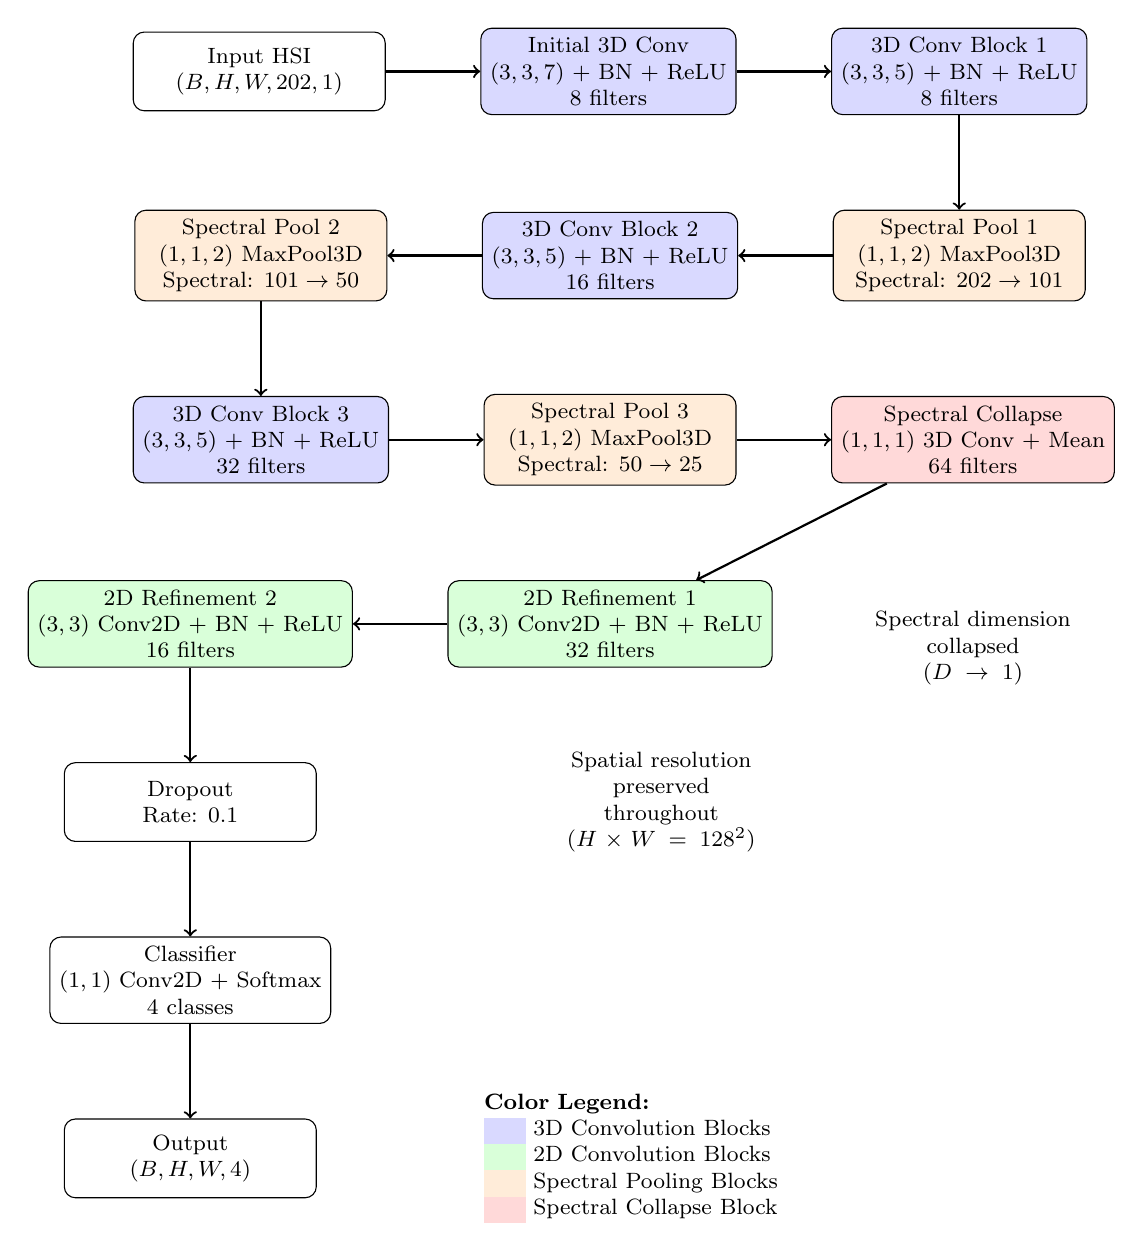
\begin{tikzpicture}[
            block/.style={draw, rounded corners, minimum width=3.2cm, minimum height=1cm, align=center, font=\footnotesize},
            conv3d/.style={draw, rounded corners, minimum width=3.2cm, minimum height=1cm, align=center, fill=blue!15, font=\footnotesize},
            conv2d/.style={draw, rounded corners, minimum width=3.2cm, minimum height=1cm, align=center, fill=green!15, font=\footnotesize},
            poolblock/.style={draw, rounded corners, minimum width=3.2cm, minimum height=1cm, align=center, fill=orange!15, font=\footnotesize},
            collapse/.style={draw, rounded corners, minimum width=3.2cm, minimum height=1cm, align=center, fill=red!15, font=\footnotesize},
            arrow/.style={->, thick},
            node distance=1.2cm
        ]

        \node[block] (input) {Input HSI\\$(B, H, W, 202, 1)$};

        \node[conv3d, right=of input] (initial) {Initial 3D Conv\\$(3,3,7)$ + BN + ReLU\\8 filters};

        \node[conv3d, right=of initial] (enc1) {3D Conv Block 1\\$(3,3,5)$ + BN + ReLU\\8 filters};

        \node[poolblock, below=of enc1] (pool1) {Spectral Pool 1\\$(1,1,2)$ MaxPool3D\\Spectral: $202 \to 101$};

        \node[conv3d, left=of pool1] (enc2) {3D Conv Block 2\\$(3,3,5)$ + BN + ReLU\\16 filters};

        \node[poolblock, left=of enc2] (pool2) {Spectral Pool 2\\$(1,1,2)$ MaxPool3D\\Spectral: $101 \to 50$};

        \node[conv3d, below=of pool2] (enc3) {3D Conv Block 3\\$(3,3,5)$ + BN + ReLU\\32 filters};

        \node[poolblock, right=of enc3] (pool3) {Spectral Pool 3\\$(1,1,2)$ MaxPool3D\\Spectral: $50 \to 25$};

        \node[collapse, right=of pool3] (collapse_conv) {Spectral Collapse\\$(1,1,1)$ 3D Conv + Mean\\$64$ filters};

        \node[conv2d, below=of pool3] (refine1) {2D Refinement 1\\$(3,3)$ Conv2D + BN + ReLU\\32 filters};

        \node[conv2d, left=of refine1] (refine2) {2D Refinement 2\\$(3,3)$ Conv2D + BN + ReLU\\16 filters};

        \node[block, below=of refine2] (dropout) {Dropout\\Rate: 0.1};

        \node[block, below=of dropout] (classifier) {Classifier\\$(1,1)$ Conv2D + Softmax\\4 classes};

        \node[block, below=of classifier] (output) {Output\\$(B, H, W, 4)$};

        % Main flow arrows
        \draw[arrow] (input) -- (initial);
        \draw[arrow] (initial) -- (enc1);
        \draw[arrow] (enc1) -- (pool1);
        \draw[arrow] (pool1) -- (enc2);
        \draw[arrow] (enc2) -- (pool2);
        \draw[arrow] (pool2) -- (enc3);
        \draw[arrow] (enc3) -- (pool3);
        \draw[arrow] (pool3) -- (collapse_conv);
        \draw[arrow] (collapse_conv) -- (refine1);
        \draw[arrow] (refine1) -- (refine2);
        \draw[arrow] (refine2) -- (dropout);
        \draw[arrow] (dropout) -- (classifier);
        \draw[arrow] (classifier) -- (output);

        % Side annotations
        \node[right=2.5cm of dropout, text width=3.5cm, align=center, font=\footnotesize] (note1) {Spatial resolution\\preserved\\throughout\\$(H \times W = 128^2)$};

        \node[below=1.5cm of collapse_conv, text width=2.5cm, align=center, font=\footnotesize] (note2) {Spectral dimension\\collapsed\\$(D \to 1)$};

        % Color legend
        \node[right=2cm of output, text width=4.5cm, align=left, font=\footnotesize] (legend) {
            \textbf{Color Legend:}\\
            \colorbox{blue!15}{\phantom{xx}} 3D Convolution Blocks\\
            \colorbox{green!15}{\phantom{xx}} 2D Convolution Blocks\\
            \colorbox{orange!15}{\phantom{xx}} Spectral Pooling Blocks\\
            \colorbox{red!15}{\phantom{xx}} Spectral Collapse Block
        };

    \end{tikzpicture}
    \caption{Small segmentation model architecture for memory-efficient HSI segmentation. The model progressively reduces spectral dimensionality while preserving full spatial resolution for per-pixel classification.}
    \label{fig:small_segmenter_architecture}
\end{figure}

\section{Training}
The model was trained on hyperspectral images with corresponding segmentation maps using categorical cross-entropy loss and the Adam optimizer.
The training process was set to run for 80 epochs, with a learning rate of 0.001.
The training and validation metrics over epochs are shown in Figure \ref{fig:small_seg_training_metrics}.
It is clear that both the training and validation loss decrease over time, while the accuracy metrics increase, indicating that the model is learning effectively without signs of overfitting.
There is, however, still some room for improvement, as the validation loss and accuracy metrics have not yet plateaued, suggesting that further training could yield better performance.
However, due to both time and computational resource constraints, it was not feasible to continue training for more epochs to explore this potential improvement.

\begin{figure}
    \centering

    \begin{subfigure}{0.45\textwidth}
        \centering
        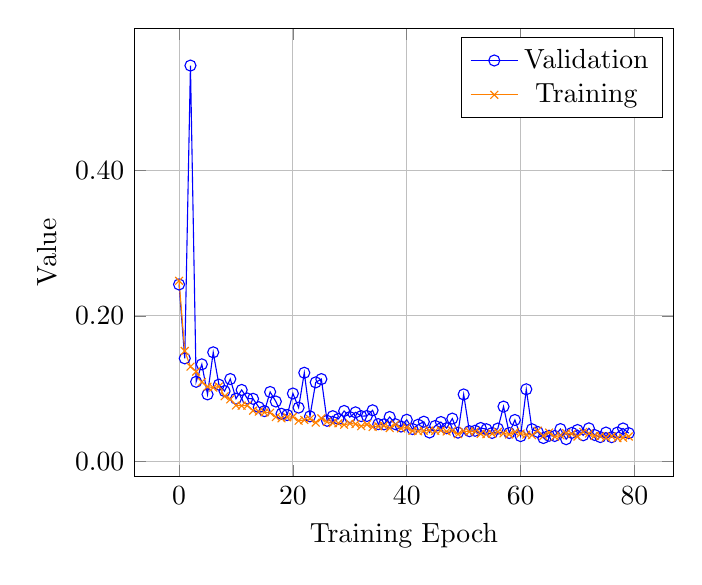
\begin{tikzpicture}
            \begin{axis}[
                    xlabel={Training Epoch},
                    ylabel={Value},
                    grid=major,
                    y tick label style={
                            /pgf/number format/.cd,
                            fixed,
                            fixed zerofill,
                            precision=2,
                            /tikz/.cd
                        },
                    x tick label style={
                            /pgf/number format/.cd,
                            fixed,
                            fixed zerofill,
                            precision=0,
                            /tikz/.cd
                        }
                ]

                \addplot [color=blue, mark=o] coordinates {
                        (0, 0.2432)
                        (1, 0.1416)
                        (2, 0.5441)
                        (3, 0.1094)
                        (4, 0.1334)
                        (5, 0.0921)
                        (6, 0.1499)
                        (7, 0.1055)
                        (8, 0.0966)
                        (9, 0.1132)
                        (10, 0.0862)
                        (11, 0.0982)
                        (12, 0.0864)
                        (13, 0.086)
                        (14, 0.0745)
                        (15, 0.0691)
                        (16, 0.0954)
                        (17, 0.0823)
                        (18, 0.0654)
                        (19, 0.0637)
                        (20, 0.0933)
                        (21, 0.0739)
                        (22, 0.1218)
                        (23, 0.0619)
                        (24, 0.1086)
                        (25, 0.1131)
                        (26, 0.0558)
                        (27, 0.0621)
                        (28, 0.0584)
                        (29, 0.0693)
                        (30, 0.0609)
                        (31, 0.0674)
                        (32, 0.0622)
                        (33, 0.0624)
                        (34, 0.0702)
                        (35, 0.0512)
                        (36, 0.0509)
                        (37, 0.061)
                        (38, 0.0511)
                        (39, 0.0479)
                        (40, 0.0572)
                        (41, 0.0445)
                        (42, 0.0504)
                        (43, 0.0545)
                        (44, 0.0397)
                        (45, 0.0487)
                        (46, 0.0541)
                        (47, 0.0456)
                        (48, 0.0588)
                        (49, 0.0395)
                        (50, 0.092)
                        (51, 0.0415)
                        (52, 0.0421)
                        (53, 0.0459)
                        (54, 0.0442)
                        (55, 0.0391)
                        (56, 0.0451)
                        (57, 0.0753)
                        (58, 0.039)
                        (59, 0.0569)
                        (60, 0.0347)
                        (61, 0.0991)
                        (62, 0.0442)
                        (63, 0.0405)
                        (64, 0.0321)
                        (65, 0.0352)
                        (66, 0.0349)
                        (67, 0.0444)
                        (68, 0.0305)
                        (69, 0.0392)
                        (70, 0.0431)
                        (71, 0.0359)
                        (72, 0.0454)
                        (73, 0.0363)
                        (74, 0.0334)
                        (75, 0.0396)
                        (76, 0.0333)
                        (77, 0.0396)
                        (78, 0.0452)
                        (79, 0.0388)
                    };
                \addlegendentry{Validation}

                \addplot [color=orange, mark=x] coordinates {
                        (0, 0.2482)
                        (1, 0.1517)
                        (2, 0.1303)
                        (3, 0.1234)
                        (4, 0.1091)
                        (5, 0.1027)
                        (6, 0.1015)
                        (7, 0.1029)
                        (8, 0.0895)
                        (9, 0.0853)
                        (10, 0.0769)
                        (11, 0.0765)
                        (12, 0.0767)
                        (13, 0.0697)
                        (14, 0.0685)
                        (15, 0.0674)
                        (16, 0.0668)
                        (17, 0.061)
                        (18, 0.0591)
                        (19, 0.0607)
                        (20, 0.0612)
                        (21, 0.0559)
                        (22, 0.0569)
                        (23, 0.0584)
                        (24, 0.0533)
                        (25, 0.0591)
                        (26, 0.0543)
                        (27, 0.0528)
                        (28, 0.0523)
                        (29, 0.0503)
                        (30, 0.052)
                        (31, 0.0513)
                        (32, 0.0484)
                        (33, 0.0508)
                        (34, 0.0473)
                        (35, 0.0482)
                        (36, 0.049)
                        (37, 0.0458)
                        (38, 0.0508)
                        (39, 0.0453)
                        (40, 0.0467)
                        (41, 0.042)
                        (42, 0.0414)
                        (43, 0.042)
                        (44, 0.0426)
                        (45, 0.0419)
                        (46, 0.0424)
                        (47, 0.0411)
                        (48, 0.0424)
                        (49, 0.0374)
                        (50, 0.0417)
                        (51, 0.0409)
                        (52, 0.0412)
                        (53, 0.038)
                        (54, 0.0374)
                        (55, 0.0381)
                        (56, 0.0405)
                        (57, 0.0385)
                        (58, 0.037)
                        (59, 0.0404)
                        (60, 0.0382)
                        (61, 0.0368)
                        (62, 0.0361)
                        (63, 0.0421)
                        (64, 0.035)
                        (65, 0.0396)
                        (66, 0.0339)
                        (67, 0.0357)
                        (68, 0.0388)
                        (69, 0.0378)
                        (70, 0.0342)
                        (71, 0.0405)
                        (72, 0.0383)
                        (73, 0.035)
                        (74, 0.0348)
                        (75, 0.0328)
                        (76, 0.0344)
                        (77, 0.032)
                        (78, 0.0326)
                        (79, 0.0342)
                    };
                \addlegendentry{Training}

            \end{axis}
        \end{tikzpicture}
        \caption{Loss over Epochs}
        \label{fig:small_sseg_loss}
    \end{subfigure}
    \hfill
    \begin{subfigure}{0.45\textwidth}
        \centering
        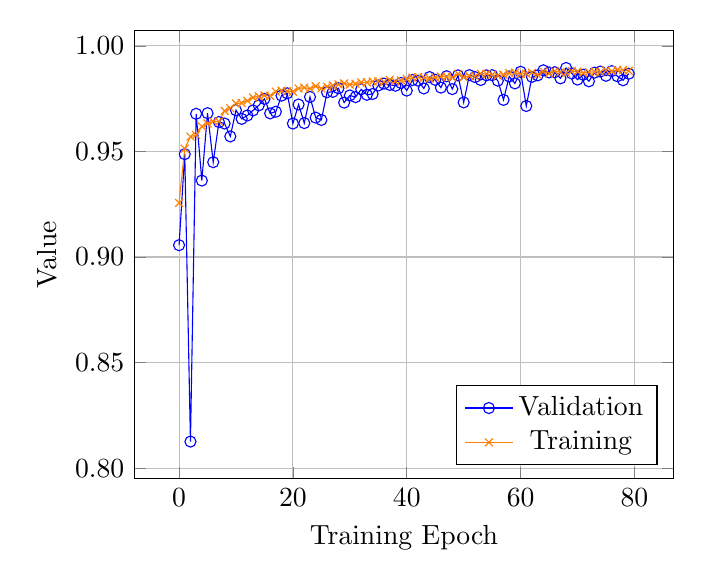
\begin{tikzpicture}
            \begin{axis}[
                    legend pos = south east,
                    xlabel={Training Epoch},
                    ylabel={Value},
                    grid=major,
                    y tick label style={
                            /pgf/number format/.cd,
                            fixed,
                            fixed zerofill,
                            precision=2,
                            /tikz/.cd
                        },
                    x tick label style={
                            /pgf/number format/.cd,
                            fixed,
                            fixed zerofill,
                            precision=0,
                            /tikz/.cd
                        }
                ]

                \addplot [color=blue, mark=o] coordinates {
                        (0, 0.9056)
                        (1, 0.9487)
                        (2, 0.8126)
                        (3, 0.9678)
                        (4, 0.9362)
                        (5, 0.9681)
                        (6, 0.9449)
                        (7, 0.9639)
                        (8, 0.9632)
                        (9, 0.9571)
                        (10, 0.9695)
                        (11, 0.9654)
                        (12, 0.967)
                        (13, 0.9694)
                        (14, 0.9718)
                        (15, 0.9749)
                        (16, 0.968)
                        (17, 0.9688)
                        (18, 0.9764)
                        (19, 0.9775)
                        (20, 0.9632)
                        (21, 0.9722)
                        (22, 0.9634)
                        (23, 0.9758)
                        (24, 0.966)
                        (25, 0.9649)
                        (26, 0.978)
                        (27, 0.9782)
                        (28, 0.9799)
                        (29, 0.9731)
                        (30, 0.9765)
                        (31, 0.9757)
                        (32, 0.9794)
                        (33, 0.9768)
                        (34, 0.9772)
                        (35, 0.9812)
                        (36, 0.9821)
                        (37, 0.9815)
                        (38, 0.9811)
                        (39, 0.9824)
                        (40, 0.9788)
                        (41, 0.9838)
                        (42, 0.9835)
                        (43, 0.9798)
                        (44, 0.9852)
                        (45, 0.9839)
                        (46, 0.9802)
                        (47, 0.9856)
                        (48, 0.9795)
                        (49, 0.986)
                        (50, 0.9732)
                        (51, 0.9861)
                        (52, 0.9852)
                        (53, 0.9838)
                        (54, 0.986)
                        (55, 0.9861)
                        (56, 0.9835)
                        (57, 0.9744)
                        (58, 0.9855)
                        (59, 0.9822)
                        (60, 0.9877)
                        (61, 0.9715)
                        (62, 0.9853)
                        (63, 0.986)
                        (64, 0.9884)
                        (65, 0.9874)
                        (66, 0.9875)
                        (67, 0.9846)
                        (68, 0.9895)
                        (69, 0.9869)
                        (70, 0.984)
                        (71, 0.9863)
                        (72, 0.9832)
                        (73, 0.9873)
                        (74, 0.9878)
                        (75, 0.9858)
                        (76, 0.988)
                        (77, 0.9856)
                        (78, 0.9837)
                        (79, 0.9868)
                    };
                \addlegendentry{Validation}

                \addplot [color=orange, mark=x] coordinates {
                        (0, 0.9256)
                        (1, 0.9513)
                        (2, 0.957)
                        (3, 0.9578)
                        (4, 0.9618)
                        (5, 0.9632)
                        (6, 0.9642)
                        (7, 0.9641)
                        (8, 0.9692)
                        (9, 0.9705)
                        (10, 0.9727)
                        (11, 0.9729)
                        (12, 0.974)
                        (13, 0.9755)
                        (14, 0.9761)
                        (15, 0.9765)
                        (16, 0.9763)
                        (17, 0.9783)
                        (18, 0.9788)
                        (19, 0.9785)
                        (20, 0.9783)
                        (21, 0.9798)
                        (22, 0.9802)
                        (23, 0.9797)
                        (24, 0.9809)
                        (25, 0.9798)
                        (26, 0.9807)
                        (27, 0.9812)
                        (28, 0.9817)
                        (29, 0.9822)
                        (30, 0.9816)
                        (31, 0.982)
                        (32, 0.9827)
                        (33, 0.9827)
                        (34, 0.9831)
                        (35, 0.9832)
                        (36, 0.9829)
                        (37, 0.9839)
                        (38, 0.9831)
                        (39, 0.9836)
                        (40, 0.9843)
                        (41, 0.9849)
                        (42, 0.9852)
                        (43, 0.985)
                        (44, 0.9845)
                        (45, 0.985)
                        (46, 0.9854)
                        (47, 0.9854)
                        (48, 0.9851)
                        (49, 0.9867)
                        (50, 0.9852)
                        (51, 0.9857)
                        (52, 0.9856)
                        (53, 0.9868)
                        (54, 0.9867)
                        (55, 0.9863)
                        (56, 0.9859)
                        (57, 0.9863)
                        (58, 0.9871)
                        (59, 0.9873)
                        (60, 0.9867)
                        (61, 0.9868)
                        (62, 0.9873)
                        (63, 0.9863)
                        (64, 0.9878)
                        (65, 0.9869)
                        (66, 0.988)
                        (67, 0.9875)
                        (68, 0.9871)
                        (69, 0.988)
                        (70, 0.9879)
                        (71, 0.9872)
                        (72, 0.9876)
                        (73, 0.9876)
                        (74, 0.9876)
                        (75, 0.9884)
                        (76, 0.988)
                        (77, 0.9886)
                        (78, 0.9885)
                        (79, 0.9882)
                    };
                \addlegendentry{Training}

            \end{axis}
        \end{tikzpicture}
        \caption{Accuracy over Epochs}
        \label{fig:small_seg_acc}
    \end{subfigure}

    \caption{Training and Validation Metrics over Epochs for the Small Segmentation model}
    \label{fig:small_seg_training_metrics}
\end{figure}

\section{Summary}
The small segmentation model works well as a symbolic representation of the next step in the data processing pipeline, which uses compression as a pre-processing step for downstream tasks such as segmentation.
The model itself is simple with a straightforward architecture that still manages to use both spatial and spectral features effectively.

% % TODO
\chapter{Verification and validation}

\section{Evaluation metrics for image compression}\label{sec:eval_metrics}
For evaluating the performance of training and validating image compression models, appropriate metrics are needed to quantify the quality of compressed images.
Some of the most common metrics used in HSI compression are Peak Signal-to-Noise Ratio (PSNR), Structural Similarity Index Measure (SSIM), Mean Squared Error (MSE), and Spectral Angle (SA)\cite{mohammadi2025evaluationobjectiveimagequality, SA}.
These metrics help to quantify the differences between the original and reconstructed images, providing insights into the effectiveness of models used for compression.
Two metrics are particularly well suited for examining HSI compression performance, SA and SSIM.
PSNR and MSE are more general metrics often used in image processing tasks.
MSE measures the average squared difference between the original and reconstructed pixel values, where PSNR is MSE logarithmic scale representation expressed in decibels (dB). \cite{mohammadi2025evaluationobjectiveimagequality}
Unlike PSNR and the MSE, SSIM is a metric designed to align more closely with visual perception.
SSIM evaluates the similarity between two images based on their structural information, luminance, and contrast. \cite{mohammadi2025evaluationobjectiveimagequality}
SA measures the spectral similarity between the original and reconstructed image by calculating the angle between their spectral vectors. \cite{SA}

\subsection{Structural Similarity Index Measure}
The Structural Similarity Index Measure (SSIM) is a metric that quantifies many image quality aspects.
It combines data about the differences in luminance, contrast, and structure between two images into a single value.
The formula for calculating SSIM between two images \( x \) and \( y \) is given by equation \ref{fig:ssim_equation}:
\begin{align}
    \text{SSIM}(x, y) = \frac{(2\mu_x \mu_y + C_1)(2\sigma_{xy} + C_2)}{(\mu_x^2 + \mu_y^2 + C_1)(\sigma_x^2 + \sigma_y^2 + C_2)}
    \label{fig:ssim_equation}
\end{align}
where \( \mu_x \) and \( \mu_y \) are the average pixel values of images \( x \) and \( y \), \( \sigma_x^2 \) and \( \sigma_y^2 \) are the variances, \( \sigma_{xy} \) is the covariance between the two images, and \( C_1 \) and \( C_2 \) are constants to ensure no division by zero takes place.
The SSIM value theoretically ranges from -1 to 1, where a value of 1 indicates perfect similarity between the two images, while values close to 0 indicate low similarity and negative values indicate very opposite similarity.
In practice, for image compression tasks, SSIM values are typically between 0 and 1, with higher values indicating better reconstruction quality.
\subsection{Spectral Angle}
The formula for calculating the SA between two spectral vectors \( \mathbf{a} \) and \( \mathbf{b} \) is given by equation \ref{fig:sa_equation}:
\begin{align}
    \text{SA}(\mathbf{a}, \mathbf{b}) = \arccos\left(\frac{\mathbf{a} \cdot \mathbf{b}}{\|\mathbf{a}\|\|\mathbf{b}\|}\right)
    \label{fig:sa_equation}
\end{align}
where \( \mathbf{a} \cdot \mathbf{b} \) is the dot product of the vectors, and \( \|\mathbf{a}\| \) and \( \|\mathbf{b}\| \) are the magnitudes of the vectors.
SA is typically measured in degrees, with smaller angles indicating greater similarity between the spectral signatures.
\subsection{Mean Squared Error}
Mean Squared Error (MSE) is a common metric often used in machine learning.
It measures the average square of the difference of each point.
In the case of images, it measures the average squared difference between the original and reconstructed pixel values.
The formula for calculating MSE between two images \( x \) and \( y \) is shown in equation \ref{fig:mse_equation}:
\begin{align}
    \text{MSE}(x, y) = \frac{1}{N} \sum_{i=1}^{N} (x_i - y_i)^2
    \label{fig:mse_equation}
\end{align}
where \( N \) is the total number of pixels in the images, and \( x_i \) and \( y_i \) are the pixel values at position \( i \).
The MSE value is non-negative, with lower values indicating better reconstruction quality.
\subsection{Peak Signal-to-Noise Ratio}
Peak Signal-to-Noise Ratio (PSNR) is a metric used to measure the quality of reconstructed images compared to the original images.
It is expressed in decibels (dB) which are logarithmic units.
This, in turn, means that small changes in PSNR can represent significant differences in image quality.
The formula for calculating PSNR between two images \( x \) and \( y \) is given by equation \ref{fig:psnr_equation}:
\begin{align}
    \text{PSNR}(x, y) = 10 \cdot \log_{10} \left( \frac{MAX_I^2}{\text{MSE}(x, y)} \right)
    \label{fig:psnr_equation}
\end{align}
where \( MAX_I \) is the maximum possible pixel value of the image.
The PSNR value is better when it is higher, with values above 30 dB generally considered good enough for most image compression tasks, while values above 45 dB are considered excellent.
It is important to note that PSNR is a logarithmic measure, so a small increase in PSNR can correspond to a significant improvement in image quality.
\subsection{Bits per pixel per channel}
Another metric specific to HSIs is the bits per pixel per channel (bpppc), which represents the average number of bits used to encode each pixel in each spectral channel.
The formula for calculating bpppc is given by equation \ref{fig:bpppc_equation}:
\begin{align}
    \text{bpppc} = \frac{\text{Total Bits in Compressed Image}}{\text{Number of Pixels} \times \text{Number of Spectral Channels}}
    \label{fig:bpppc_equation}
\end{align}
The bpppc metric is particularly important for evaluating the efficiency of compression algorithms, as it directly relates to the amount of data required to represent the image.
Lower bpppc values indicate more efficient compression, while higher values indicate less efficient compression.

\subsection{Error histogram}
Besides numerical metrics, visualizing the distribution of reconstruction errors was employed to gain insights into the typical errors made by the compression models.
Visualizing the distribution of reconstruction errors can be achieved in the form of a histogram.
The histograms present the frequency of errors over some interval, which provides a way to identify patterns in the errors.
For instance, a histogram that is heavily skewed toward zero indicates that most reconstruction errors are small, suggesting that the model is performing well.
A histogram with a peak away from zero indicates that the model is frequently making larger errors, which may suggest areas for improvement.
The best error histogram would ideally show a high frequency of errors close to zero, indicating that the model is accurately reconstructing the images with minimal errors.

\subsection{Error map}
An additional method for visualizing reconstruction errors is through error maps.
Error maps are the result of calculating the difference between the original and reconstructed images on a pixel-by-pixel basis.
These maps provide a spatial representation of where the model is performing well and where it is struggling.
The error maps presented in this thesis use a color scale to represent the magnitude of the errors.
Pixels with negative errors are shown in shades of blue, while pixels with positive errors are shown in shades of red, and black represents zero error.
This color scheme allows for easy identification of areas where the model is overestimating or underestimating pixel values.

\section{Evaluation of semantic segmentation} \label{sec:segmentation_eval}
To evaluate the performance of the semantic segmentation model, several common metrics were used, including the confusion matrix, accuracy, positive predictive value (PPV), recall, F1-score, Intersection over Union (IoU), and Area under Curve (AUC).
These metrics provide a comprehensive assessment of the model's ability to correctly assign classes to each pixel in the image.
% ROZWINAC

\subsection{Confusion matrix}
A confusion matrix is a table that summarizes the performance of a classification model by comparing the predicted class labels with the true class labels.
Each row of the matrix corresponds to the true class (as labeled in the dataset), while each column corresponds to the predicted class (as output by the model).
The entries in the matrix represent the number of pixels that were classified into each combination of true and predicted classes.
The perfect model would produce a diagonal confusion matrix, where all pixels are correctly classified into their respective classes.\par
The confusion matrix provides a detailed view of the model's performance, allowing for the identification of specific classes that may be more challenging to classify correctly.
Another useful aspect of the confusion matrix is that it can be used to calculate other evaluation metrics such as accuracy, precision, recall, and F1-score.
This can be done by summing the appropriate entries in the matrix to obtain the necessary counts for each metric.
All of these summations fall into four categories: true positives (TP), true negatives (TN), false positives (FP), and false negatives (FN).
True positives are the number of pixels that were correctly classified as belonging to a particular class.
True negatives are the number of pixels that were correctly classified as not belonging to a particular class.
False positives are the number of pixels that were incorrectly classified as belonging to a particular class when they do not.
False negatives are the number of pixels that were incorrectly classified as not belonging to a particular class when they do.

\subsection{Accuracy}
Accuracy is a metric that measures the overall correctness of the model's predictions.
It is calculated as the ratio of correctly classified pixels to the total number of pixels in the image.
The formula for calculating accuracy is given by equation \ref{fig:accuracy_equation}:
\begin{align}
    \text{Accuracy} = \frac{TP + TN}{TP + TN + FP + FN}
    \label{fig:accuracy_equation}
\end{align}
The accuracy value ranges from 0 to 1, with higher values indicating better performance.

\subsection{Positive predictive value }
PPV is a metric that directly measures the proportion of positive identifications that were actually correct.
It is calculated as the ratio of true positives to the sum of true positives and false positives.
The formula for calculating PPV is given by equation \ref{fig:ppv_equation}:
\begin{align}
    \text{PPV} = \frac{TP}{TP + FP}
    \label{fig:ppv_equation}
\end{align}
The PPV value ranges from 0 to 1, with higher values indicating better performance.
\subsection{Recall}
Recall is a metric that measures the model's ability to correctly identify all relevant instances of a particular class.
It is calculated as the ratio of true positives to the sum of true positives and false negatives.
The formula for calculating recall is given by equation \ref{fig:recall_equation}:
\begin{align}
    \text{Recall} = \frac{TP}{TP + FN}
    \label{fig:recall_equation}
\end{align}
The recall value ranges from 0 to 1, with higher values indicating better performance.
\subsection{F1-score}
F1-score is a metric that combines PPV and recall into a single value.
It is the harmonic mean of PPV and recall, providing a balanced measure of the model's performance.
The formula for calculating F1-score is given by equation \ref{fig:f1_equation}:
\begin{align}
    \text{F1-score} = 2 \cdot \frac{\text{PPV} \cdot \text{Recall}}{\text{PPV} + \text{Recall}}
    \label{fig:f1_equation}
\end{align}
The F1-score value ranges from 0 to 1, with higher values indicating better performance.
\subsection{Intersection over Union}
IoU is a metric that measures the overlap between the predicted and true class labels.
It is calculated as the ratio of the intersection of the predicted and true class labels to the union of the predicted and true class labels.
The formula for calculating IoU is given by equation \ref{fig:iou_equation}:
\begin{align}
    \text{IoU} = \frac{TP}{TP + FP + FN}
    \label{fig:iou_equation}
\end{align}
The IoU value ranges from 0 to 1, with higher values indicating better performance.
\subsection{Area under Curve}
AUC is a metric that measures the model's ability to distinguish between different classes.
It is calculated as the area under the Receiver Operating Characteristic (ROC) curve, which plots the true positive rate against the false positive rate at various threshold settings.
AUC values range from 0 to 1, with higher values indicating better performance.
It is particularly useful for evaluating models in imbalanced datasets, where one class may be more prevalent than others.
AUC is calculated using numerical integration methods, such as the Riemann sum or trapezoidal rule, to estimate the area under the ROC curve.
The formula for calculating AUC is given by equation \ref{fig:auc_equation}:
\begin{align}
    \text{AUC} = \int_{0}^{1} \text{TPR}(t) \, d\text{FPR}(t)
    \label{fig:auc_equation}
\end{align}
The perfect model would have an AUC of 1, which means that the model is able to distinguish classes with perfect accuracy and a random model would have an AUC of 0.5 (for a balanced dataset), which means that the model is no better than random guessing.

\section{Segmentation model evaluation}
To evaluate the performance of the semantic segmentation model, the metrics mentioned in Section \ref{sec:segmentation_eval} were calculated using the model's predictions on the test dataset.
These metrics were first calculated for the uncompressed images to establish a baseline performance for the model.
Subsequently, the same metrics were calculated for the images reconstructed from each compression model, which will be further discussed in the section about each model.
In addition to numerical metrics, confusion matrices were generated for both the uncompressed and reconstructed images to visually compare the model's performance across different classes.
This comprehensive evaluation approach allowed for a thorough assessment of the impact of compression on the semantic segmentation model's performance.
The model achieved the results shown in Table \ref{tab:orig_seg_metrics} when evaluated on the uncompressed test dataset.
These were calculated from the confusion matrix shown in Figure \ref{fig:orig_confusion_matrix}.
The metrics over all classes are in the Table \ref{tab:orig_seg_metrics_avg}.
\begin{table}[h!]
    \centering
    \caption{Semantic segmentation model evaluation metrics on uncompressed test dataset over all classes}
    \label{tab:orig_seg_metrics_avg}
    \begin{tabular}{m{10em}| m{10em}}
        \toprule
        Metric   & Average Value      \\
        \midrule
        Accuracy & 0.9893 \\
        F1-Score & 0.9042 \\
        IoU      & 0.8446 \\
        AUC      & 0.8735 \\
        \bottomrule
    \end{tabular}
\end{table}

\begin{table}[h!]
    \centering
    \caption{Semantic segmentation model evaluation metrics on uncompressed test dataset per class}
    \label{tab:orig_seg_metrics}
    \begin{tabular}{m{7em}| m{7em} m{7em} m{7em}}
        \toprule
        Metric   & Value for class 0 & Value for class 1 & Value for class 2 \\
        \midrule
        PPV      & 0.8389   & 0.9911   & 0.9876   \\
        Recall   & 0.6608   & 0.9966   & 0.9715   \\
        F1-Score & 0.7393   & 0.9939   & 0.9795   \\
        IoU      & 0.5864   & 0.9878   & 0.9598   \\
        \bottomrule
    \end{tabular}
\end{table}

\begin{figure}[htbp]
    \centering
    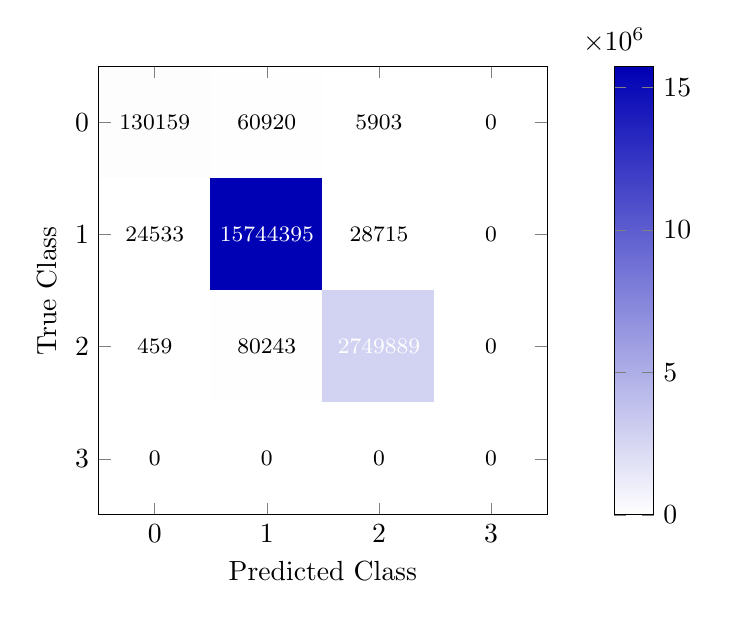
\begin{tikzpicture}
        \begin{axis}[
                width=0.6\textwidth,
                height=0.6\textwidth,
                view={0}{90},
                colormap={whiteblue}{rgb255(0cm)=(255,255,255); rgb255(1cm)=(0,0,180)},
                colorbar right,
                colorbar style={
                        at={(1.15,0.5)},
                        anchor=west,
                        scaled y ticks=base 10:-6,
                        ytick scale label code/.code={$\times 10^{6}$},
                    },
                xlabel={Predicted Class},
                ylabel={True Class},
                xtick={0,1,2,3},
                ytick={0,1,2,3},
                xticklabels={0, 1, 2, 3},
                yticklabels={0, 1, 2, 3},
                y dir=reverse,
                enlargelimits=false,
                point meta min=0,
                point meta max=15744395,
            ]
            \addplot[
                matrix plot,
                mesh/cols=4,
                point meta=explicit,
            ] coordinates {
                    (0,0) [130159]   (1,0) [60920]     (2,0) [5903]      (3,0) [0]
                    (0,1) [24533]    (1,1) [15744395]  (2,1) [28715]     (3,1) [0]
                    (0,2) [459]      (1,2) [80243]     (2,2) [2749889]   (3,2) [0]
                    (0,3) [0]        (1,3) [0]         (2,3) [0]         (3,3) [0]
                };
            % Add numerical labels
            \node at (axis cs:0,0) {\footnotesize 130159};
            \node at (axis cs:1,0) {\footnotesize 60920};
            \node at (axis cs:2,0) {\footnotesize 5903};
            \node at (axis cs:3,0) {\footnotesize 0};
            \node at (axis cs:0,1) {\footnotesize 24533};
            \node[white] at (axis cs:1,1) {\footnotesize 15744395};
            \node at (axis cs:2,1) {\footnotesize 28715};
            \node at (axis cs:3,1) {\footnotesize 0};
            \node at (axis cs:0,2) {\footnotesize 459};
            \node at (axis cs:1,2) {\footnotesize 80243};
            \node[white] at (axis cs:2,2) {\footnotesize 2749889};
            \node at (axis cs:3,2) {\footnotesize 0};
            \node at (axis cs:0,3) {\footnotesize 0};
            \node at (axis cs:1,3) {\footnotesize 0};
            \node at (axis cs:2,3) {\footnotesize 0};
            \node at (axis cs:3,3) {\footnotesize 0};
        \end{axis}
    \end{tikzpicture}
    \caption{Confusion matrix heatmap for baseline segmentation on uncompressed images vs ground truth}
    \label{fig:orig_confusion_matrix}
\end{figure}

An interesting observation from the confusion matrix in Figure \ref{fig:orig_confusion_matrix} is that class 3 does not appear in the test set at all.
This means that the model was never evaluated on this class, which could potentially skew the overall performance. Upon closer inspection, it was found that it doesn't appear once in the whole dataset.
This results in our inability to calculate any meaningful metrics for this class, and thus it was omitted from both Table \ref{tab:orig_seg_metrics} and any future per class metrics tables.
Another observation is that class 0 has a significantly lower occurrence rate compared to classes 1 and 2.
This class imbalance is reflected in the model's performance, with class 0 having notably lower PPV, recall, F1-score, and IoU compared to the other two classes that exist in the dataset.
Overall, the model performs admirably on the uncompressed test dataset, achieving high scores across all metrics.
% Dodac zdjecia
\begin{figure}
    \centering
    \begin{subfigure}{0.3\textwidth}
        \includegraphics[width=\textwidth]{./graf/sample_09_input.png}
        \caption{Original image}
        \label{fig:segmentation_example_original}
    \end{subfigure}
    \hfill
    \begin{subfigure}{0.3\textwidth}
        \includegraphics[width=\textwidth]{./graf/sample_09_gt.png}
        \caption{Ground truth}
        \label{fig:segmentation_example_ground_truth}
    \end{subfigure}
    \hfill
    \begin{subfigure}{0.3\textwidth}
        \includegraphics[width=\textwidth]{./graf/sample_09_pred.png}
        \caption{Predicted segmentation}
        \label{fig:segmentation_example_prediction}
    \end{subfigure}

    \begin{subfigure}{0.3\textwidth}
        \includegraphics[width=\textwidth]{./graf/sample_39_input.png}
        \caption{Original image}
        \label{fig:segmentation_example_original_2}
    \end{subfigure}
    \hfill
    \begin{subfigure}{0.3\textwidth}
        \includegraphics[width=\textwidth]{./graf/sample_39_gt.png}
        \caption{Ground truth}
        \label{fig:segmentation_example_ground_truth_2}
    \end{subfigure}
    \hfill
    \begin{subfigure}{0.3\textwidth}
        \includegraphics[width=\textwidth]{./graf/sample_39_pred.png}
        \caption{Predicted segmentation}
        \label{fig:segmentation_example_prediction_2}
    \end{subfigure}

    \begin{subfigure}{0.3\textwidth}
        \includegraphics[width=\textwidth]{./graf/sample_12_input.png}
        \caption{Original image}
        \label{fig:segmentation_example_original_3}
    \end{subfigure}
    \hfill
    \begin{subfigure}{0.3\textwidth}
        \includegraphics[width=\textwidth]{./graf/sample_12_gt.png}
        \caption{Ground truth}
        \label{fig:segmentation_example_ground_truth_3}
    \end{subfigure}
    \hfill
    \begin{subfigure}{0.3\textwidth}
        \includegraphics[width=\textwidth]{./graf/sample_12_pred.png}
        \caption{Predicted segmentation}
        \label{fig:segmentation_example_prediction_3}
    \end{subfigure}
    \label{fig:segmentation_examples}
    \caption{Examples of semantic segmentation model predictions on uncompressed test images}

\end{figure}
\pagebreak

\section{Compression models evaluation}
\label{sec:eval}
The following subsections describe each model with metrics described in Section \ref{sec:eval_metrics}.
All of the models were evaluated on the test dataset provided in the HySpecNet-11k dataset.
All of the models were assessed using the same set of metrics for consistency and comparability.
Most models were evaluated using the easy split of the dataset, except for the RCGDNAE model, which was evaluated using the hard split.
This choice was made to ensure all of the models were tested under similar conditions, but also to ensure that no data leakage occurred between training and testing phases.
The evaluation metrics used are described in Section \ref{sec:eval_metrics} and include PSNR, SSIM, MSE, SA, bpppc, and compression ratio (CR).
All of the metrics were calculated as mean values over the entire test dataset.
In addition to numerical metrics and histograms of reconstruction errors, several examples of images from the test dataset were selected to visually compare the original and reconstructed images from each model.
Another important aspect of the evaluation was to assess the performance of the semantic segmentation model on the reconstructed images from each compression model.
This was done to measure the impact of compression on downstream tasks such as segmentation.
To this end, the segmentation model described in Chapter \ref{chap:small_segmenter} was used to predict class labels for the reconstructed images from each compression model.
The segmentation model's performance was then evaluated using the metrics described in Section \ref{sec:segmentation_eval}.
This comprehensive evaluation approach allowed for a thorough assessment of each compression model's performance, both in terms of image quality and its impact on downstream tasks.


\subsection{LineRWKV}
The metrics calculated for the LineRWKV model are shown in Table \ref{tab:LineRWKV_metrics}.
The histogram of reconstruction errors for the model is shown in Figure \ref{fig:linerwkv_hist}.
The error map for the best reconstructed image is shown in Figures \ref{fig:linerwkv_best}.\par


\begin{table}[h!]
    \centering
    \caption{LineRWKV evaluation metrics}
    \label{tab:LineRWKV_metrics}
    \begin{tabular}{m{20em}| m{10em}}
        \toprule
        Metric       & Value                  \\
        \midrule
        PSNR (dB)    & 44.87                  \\
        SSIM         & 0.985                  \\
        MSE          & \(3.9 \times 10^{-5}\) \\
        SA (degrees) & 3.987                  \\
        bpppc        & 2.00                   \\
        CR           & 8.00                   \\
        \bottomrule
    \end{tabular}
\end{table}

\begin{figure}
    \centering
    \begin{tikzpicture}
        \begin{axis}[
                width=1\textwidth,
                height=0.8\textwidth,
                xlabel={Reconstruction Error},
                ylabel={Occurrences},
                ybar,
                bar width=1.2pt,
                bar shift=0pt,
                % xtick={-0.02, 0,0.02, 0.04,0.06, 0.08, 0.1, 0.12, 0.13, 0.14, 0.15},
                ymin=0,
                xmin=0,
                grid=major,
            ]
            \addplot [blue, fill=blue]
            table[x index=0, y index=1] {./../results/histograms/LineRWKV.txt};
        \end{axis}
    \end{tikzpicture}
    \caption{Histogram reconstruction error for LineRWKV}
    \label{fig:linerwkv_hist}
\end{figure}


\begin{figure}
    \centering
    \begin{subfigure}{0.45\textwidth}
        \includegraphics[width=\textwidth]{./../results/histograms/RWKV/images/best_original_254.png}
        \caption{Original image}
        \label{fig:linerwkv_best_original}
    \end{subfigure}
    \hfill
    \begin{subfigure}{0.45\textwidth}
        \includegraphics[width=\textwidth]{./../results/histograms/RWKV/images/best_reconstructed_254.png}
        \caption{Reconstructed image}
        \label{fig:linerwkv_best_reconstructed}
    \end{subfigure}
    \par\medskip
    \begin{subfigure}{0.45\textwidth}
        \begin{tikzpicture}
            \node[anchor=south west,inner sep=0] (image) at (0,0) {
                \includegraphics[width=0.85\textwidth]{./../results/histograms/RWKV/images/best_error_map_254_min_-2.196178e-03_max_1.272906e-03.png}
            };
            \begin{axis}[
                at={(image.south east)},
                anchor=south west,
                width=0.12\textwidth,
                height=0.85\textwidth,
                hide axis,
                scale only axis,
                colorbar right,
                colormap={blueblackredzeroed}{
                    color(-2.196178e-03)=(blue);
                    color(0)=(black);
                    color(1.272906e-03)=(red)
                },
                point meta min=-2.196178e-03,
                point meta max=1.272906e-03,
                colorbar style={
                    ylabel={Error},
                    ylabel style={rotate=0}
                }
            ]
            \end{axis}
        \end{tikzpicture}
        \caption{Per pixel error map normalized to between $-2.1962 \times 10^{-3}$ and $1.2729 \times 10^{-3}$}
        \label{fig:linerwkv_best_error_map}
    \end{subfigure}
    \hfill
    \begin{subfigure}{0.5\textwidth}
        \centering
        \begin{tikzpicture}
            \begin{axis}[
                    width=1\textwidth,
                    height=1\textwidth,
                    xlabel={Error},
                    ylabel={Occurrences},
                    ybar,
                bar width=1.2pt,
                bar shift=0pt,
                    ymin=0,
                    grid=major,
                ]
                \addplot [blue, fill=blue]
                table[x index=0, y index=1] {./../results/histograms/RWKV/plots/pixel_error_hist_best_254.txt};
            \end{axis}
        \end{tikzpicture}
        \caption{Per pixel error histogram}
        \label{fig:linerwkv_best_hist}
    \end{subfigure}
    \caption{Best image reconstruction for LineRWKV model}
    \label{fig:linerwkv_best}
\end{figure}

\begin{figure}
    \centering
    \begin{subfigure}{0.45\textwidth}
        \includegraphics[width=\textwidth]{./../results/histograms/RWKV/images/median_original_505.png}
        \caption{Original image}
        \label{fig:linerwkv_mid_original}
    \end{subfigure}
    \hfill
    \begin{subfigure}{0.45\textwidth}
        \includegraphics[width=\textwidth]{./../results/histograms/RWKV/images/median_reconstructed_505.png}
        \caption{Reconstructed image}
        \label{fig:linerwkv_mid_reconstructed}
    \end{subfigure}
    \par\medskip
    \begin{subfigure}{0.45\textwidth}
        \begin{tikzpicture}
            \node[anchor=south west,inner sep=0] (image) at (0,0) {
                \includegraphics[width=0.85\textwidth]{./../results/histograms/RWKV/images/median_error_map_505_min_-4.545168e-03_max_1.904916e-03.png}
            };
            \begin{axis}[
                at={(image.south east)},
                anchor=south west,
                width=0.12\textwidth,
                height=0.85\textwidth,
                hide axis,
                scale only axis,
                colorbar right,
                colormap={blueblackredzeroed}{
                    color(-4.545168e-03)=(blue);
                    color(0)=(black);
                    color(1.904916e-03)=(red)
                },
                point meta min=-4.545168e-03,
                point meta max=1.904916e-03,
                colorbar style={
                    ylabel={Error},
                    ylabel style={rotate=0}
                }
            ]
            \end{axis}
        \end{tikzpicture}
        \caption{Per pixel error map normalized to between $-4.5452 \times 10^{-3}$ and $1.9049 \times 10^{-3}$}
        \label{fig:linerwkv_mid_error_map}
    \end{subfigure}
    \hfill
    \begin{subfigure}{0.5\textwidth}
        \centering
        \begin{tikzpicture}
            \begin{axis}[
                    width=1\textwidth,
                    height=1\textwidth,
                    xlabel={Error},
                    ylabel={Occurrences},
                    ybar,
                bar width=1.2pt,
                bar shift=0pt,
                    ymin=0,
                    grid=major,
                ]
                \addplot [blue, fill=blue]
                table[x index=0, y index=1] {./../results/histograms/RWKV/plots/pixel_error_hist_median_505.txt};
            \end{axis}
        \end{tikzpicture}
        \caption{Per pixel error histogram}
        \label{fig:linerwkv_mid_hist}
    \end{subfigure}
    \caption{Median image reconstruction for LineRWKV model}
    \label{fig:linerwkv_mid}
\end{figure}

\begin{figure}
    \centering
    \begin{subfigure}{0.45\textwidth}
        \includegraphics[width=\textwidth]{./../results/histograms/RWKV/images/worst_original_749.png}
        \caption{Original image}
        \label{fig:linerwkv_worst_original}
    \end{subfigure}
    \hfill
    \begin{subfigure}{0.45\textwidth}
        \includegraphics[width=\textwidth]{./../results/histograms/RWKV/images/worst_reconstructed_749.png}
        \caption{Reconstructed image}
        \label{fig:linerwkv_worst_reconstructed}
    \end{subfigure}
    \par\medskip
    \begin{subfigure}{0.45\textwidth}
        \begin{tikzpicture}
            \node[anchor=south west,inner sep=0] (image) at (0,0) {
                \includegraphics[width=0.85\textwidth]{./../results/histograms/RWKV/images/worst_error_map_749_min_-5.797678e-03_max_3.912130e-03.png}
            };
            \begin{axis}[
                at={(image.south east)},
                anchor=south west,
                width=0.12\textwidth,
                height=0.85\textwidth,
                hide axis,
                scale only axis,
                colorbar right,
                colormap={blueblackredzeroed}{
                    color(-5.797678e-03)=(blue);
                    color(0)=(black);
                    color(3.912130e-03)=(red)
                },
                point meta min=-5.797678e-03,
                point meta max=3.912130e-03,
                colorbar style={
                    ylabel={Error},
                    ylabel style={rotate=0}
                }
            ]
            \end{axis}
        \end{tikzpicture}
        \caption{Per pixel error map normalized to between $-5.7977 \times 10^{-3}$ and $3.9121 \times 10^{-3}$}
        \label{fig:linerwkv_worst_error_map}
    \end{subfigure}
    \hfill
    \begin{subfigure}{0.5\textwidth}
        \centering
        \begin{tikzpicture}
            \begin{axis}[
                    width=1\textwidth,
                    height=1\textwidth,
                    xlabel={Error},
                    ylabel={Occurrences},
                    ybar,
                bar width=1.2pt,
                bar shift=0pt,
                    ymin=0,
                    grid=major,
                ]
                \addplot [blue, fill=blue]
                table[x index=0, y index=1] {./../results/histograms/RWKV/plots/pixel_error_hist_worst_749.txt};
            \end{axis}
        \end{tikzpicture}
        \caption{Per pixel error histogram}
        \label{fig:linerwkv_worst_hist}
    \end{subfigure}
    \caption{Worst image reconstruction for LineRWKV model}
    \label{fig:linerwkv_worst}
\end{figure}




By analyzing the results, it can be assessed that the model is behaving moderately well.
It is able to reconstruct images with high fidelity, as indicated by the high PSNR and SSIM values.
The relatively low PSNR values compared to what would be expected from a lossless or near-lossless compression method stem from the low number of learning epochs used during training.
However, by applying the residuals to the base model predictions, the model is able to achieve near-lossless reconstruction quality.
This, however, comes at a cost to the compression ratio, which is lower than that of other models presented in this thesis. \par
The error histogram in Figure \ref{fig:linerwkv_hist} shows that the majority of reconstruction errors are below \(0.5 \times 10^{-2}\), which indicates that the model is able to reconstruct most images with minimal error.
The error histograms in Figures \ref{fig:linerwkv_best_hist}, \ref{fig:linerwkv_mid_hist}, and \ref{fig:linerwkv_worst_hist} show that the per pixel errors are generally small and in the shape of a normal distribution.
This is generally a good sign, as it shows that the model is good at minimizing large errors, although there exists a slight offset in the error distribution, which can be attributed to the fact that the model is not trained for a sufficient number of epochs to fully converge, which would likely result in a more centered error distribution.
An additional observation from both the histograms and the error maps shown in Figures \ref{fig:linerwkv_best_error_map}, \ref{fig:linerwkv_mid_error_map}, and \ref{fig:linerwkv_worst_error_map} is that there are a few relatively large errors that occur in the reconstructed images, which can be seen in the tails of the error histograms and the red and blue areas in the error maps.
These large errors mostly occur in the beginnings of the images, which is expected, as the model operates on the principle of predicting the next pixel based on the previous ones, which makes the beginning of the images more difficult to reconstruct accurately.\par
The metrics for the segmentation model using the images after compressing and decompressing with the LineRWKV model are shown in tables \ref{tab:seg_metrics_linerwkv} and \ref{tab:seg_metrics_linerwkv_individual}.
These metrics were calculated from the confusion matrix shown in Figure \ref{fig:linerwkv_confusion_matrix}.
The results indicate that the segmentation model performs well on the processed images, albeit with a slight decrease in performance compared to the baseline results on uncompressed images.
This suggests that the LineRWKV model is able to preserve important features in the images that are crucial for downstream tasks such as segmentation.



\begin{table}[h!]
    \centering
    \caption{Average segmentation metrics for LineRWKV reconstructed images}
    \label{tab:seg_metrics_linerwkv}
    \begin{tabular}{m{10em}| m{10em}}
        \toprule
        Metric   & Value  \\
        \midrule
        Accuracy & 0.9645 \\
        F1-score & 0.8394 \\
        IoU      & 0.7490 \\
        AUC      & 0.8674 \\
        \bottomrule
    \end{tabular}
\end{table}

\begin{table}[h!]
    \centering
    \caption{Per class segmentation metrics for LineRWKV reconstructed images}
    \label{tab:seg_metrics_linerwkv_individual}
    \begin{tabular}{m{7em}| m{7em} m{7em} m{7em} m{7em}}
        \toprule
        Metric   & Value for class 0 & Value for class 1 & Value for class 2 \\
        \midrule
        PPV      & 0.6863            & 0.9701            & 0.9478            \\
        Recall   & 0.5974            & 0.9882            & 0.8573            \\
        F1-Score & 0.6388            & 0.9791            & 0.9003            \\
        IoU      & 0.4693            & 0.9590            & 0.8187            \\
        \bottomrule
    \end{tabular}
\end{table}

\begin{figure}[htbp]
    \centering
    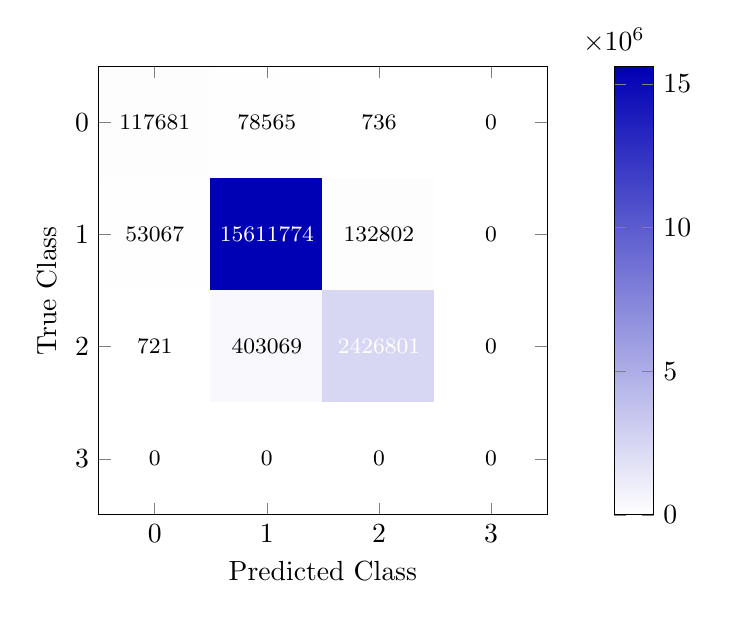
\begin{tikzpicture}
        \begin{axis}[
                width=0.6\textwidth,
                height=0.6\textwidth,
                view={0}{90},
                colormap={whiteblue}{rgb255(0cm)=(255,255,255); rgb255(1cm)=(0,0,180)},
                colorbar right,
                colorbar style={
                        at={(1.15,0.5)},
                        anchor=west,
                        scaled y ticks=base 10:-6,
                        ytick scale label code/.code={$\times 10^{6}$},
                    },
                xlabel={Predicted Class},
                ylabel={True Class},
                xtick={0,1,2,3},
                ytick={0,1,2,3},
                xticklabels={0, 1, 2, 3},
                yticklabels={0, 1, 2, 3},
                y dir=reverse,
                enlargelimits=false,
                point meta min=0,
                point meta max=15611774,
            ]
            \addplot[
                matrix plot,
                mesh/cols=4,
                point meta=explicit,
            ] coordinates {
                    (0,0) [117681]   (1,0) [78565]     (2,0) [736]       (3,0) [0]
                    (0,1) [53067]    (1,1) [15611774]  (2,1) [132802]    (3,1) [0]
                    (0,2) [721]      (1,2) [403069]    (2,2) [2426801]   (3,2) [0]
                    (0,3) [0]        (1,3) [0]         (2,3) [0]         (3,3) [0]
                };
            % Add numerical labels
            \node at (axis cs:0,0) {\footnotesize 117681};
            \node at (axis cs:1,0) {\footnotesize 78565};
            \node at (axis cs:2,0) {\footnotesize 736};
            \node at (axis cs:3,0) {\footnotesize 0};
            \node at (axis cs:0,1) {\footnotesize 53067};
            \node[white] at (axis cs:1,1) {\footnotesize 15611774};
            \node at (axis cs:2,1) {\footnotesize 132802};
            \node at (axis cs:3,1) {\footnotesize 0};
            \node at (axis cs:0,2) {\footnotesize 721};
            \node at (axis cs:1,2) {\footnotesize 403069};
            \node[white] at (axis cs:2,2) {\footnotesize 2426801};
            \node at (axis cs:3,2) {\footnotesize 0};
            \node at (axis cs:0,3) {\footnotesize 0};
            \node at (axis cs:1,3) {\footnotesize 0};
            \node at (axis cs:2,3) {\footnotesize 0};
            \node at (axis cs:3,3) {\footnotesize 0};
        \end{axis}
    \end{tikzpicture}
    \caption{Confusion matrix heatmap for LineRWKV reconstructed images vs ground truth}
    \label{fig:linerwkv_confusion_matrix}
\end{figure}

\pagebreak
\subsection{Residual Convolutional 3D Autoencoder }
The reconstruction results for RCAE3D model are shown in Table \ref{tab:CAE3D_metrics}.
The histogram of reconstruction errors for RCAE3D model is shown in Figure \ref{fig:cae3d_hist}.
The best reconstructed image as well as its error map are shown in Figure \ref{fig:cae3d_best}.\par

\begin{table}[h!]
    \centering
    \caption{RCAE3D evaluation metrics}
    \label{tab:CAE3D_metrics}
    \begin{tabular}{m{20em}| m{10em}}
        \toprule
        Metric       & Value                   \\
        \midrule
        PSNR (dB)    & 38.1504                 \\
        SSIM         & 0.9774                  \\
        MSE          & \(1.89 \times 10^{-4}\) \\
        SA (degrees) & 5.138                   \\
        bpppc        & 1.2673                  \\
        CR           & 12.6253                 \\
        \bottomrule
    \end{tabular}
\end{table}


\begin{figure}[htbp]
    \centering
    \begin{tikzpicture}
        \begin{axis}[
                width=1\textwidth,
                height=0.8\textwidth,
                xlabel={Reconstruction Error},
                ylabel={Occurrences},
                ybar,
                bar width=1.2pt,
                bar shift=0pt,
                xtick={-0.02, 0,0.02, 0.04,0.06, 0.08, 0.1, 0.12, 0.13, 0.14, 0.15},
                ymin=0,
                xmin=0,
                grid=major,
            ]
            \addplot [blue, fill=blue]
            table[x index=0, y index=1] {./graf/cae3D_histogram_data.txt};
        \end{axis}
    \end{tikzpicture}
    \caption{Histogram reconstruction error for RCAE3D}
    \label{fig:cae3d_hist}
\end{figure}


\begin{figure}[htbp]
    \centering
    \begin{subfigure}{0.45\textwidth}
        \includegraphics[width=\textwidth]{./../results/histograms/cae3D/images/best_original_250.png}
        \caption{Original image}
        \label{fig:cae3d_best_original}
    \end{subfigure}
    \hfill
    \begin{subfigure}{0.45\textwidth}
        \includegraphics[width=\textwidth]{./../results/histograms/cae3D/images/best_reconstructed_250.png}
        \caption{Reconstructed image}
        \label{fig:cae3d_best_reconstructed}
    \end{subfigure}
    \par\medskip
    \begin{subfigure}{0.45\textwidth}
        \begin{tikzpicture}
            \node[anchor=south west,inner sep=0] (image) at (0,0) {
                \includegraphics[width=0.85\textwidth]{./../results/histograms/cae3D/images/best_error_map_250_min_-7.727822e-02_max_9.891923e-02.png}
            };
            \begin{axis}[
                at={(image.south east)},
                anchor=south west,
                width=0.12\textwidth,
                height=0.85\textwidth,
                hide axis,
                scale only axis,
                colorbar right,
                colormap={blueblackredzeroed}{
                    color(-7.727822e-02)=(blue);
                    color(0)=(black);
                    color(9.891923e-02)=(red)
                },
                point meta min=-7.727822e-02,
                point meta max=9.891923e-02,
                colorbar style={
                    ylabel={Error},
                    ylabel style={rotate=0}
                }
            ]
            \end{axis}
        \end{tikzpicture}
        \caption{Per pixel error map normalized to between $-7.7278 \times 10^{-2}$ and $9.8919 \times 10^{-2}$}
        \label{fig:cae3d_best_error_map}
    \end{subfigure}
    \hfill
    \begin{subfigure}{0.5\textwidth}
        \centering
        \begin{tikzpicture}
            \begin{axis}[
                    width=1\textwidth,
                    height=1\textwidth,
                    xlabel={Error},
                    ylabel={Occurrences},
                    ybar,
                    bar width=1.2pt,
                    bar shift=0pt,
                    ymin=0,
                    grid=major,
                ]
                \addplot [blue, fill=blue]
                table[x index=0, y index=1] {./../results/histograms/cae3D/plots/pixel_error_hist_best_250.txt};
            \end{axis}
        \end{tikzpicture}
        \caption{Per pixel error histogram}
        \label{fig:cae3d_best_hist}
    \end{subfigure}
    \caption{Best image reconstruction for RCAE3D model}
    \label{fig:cae3d_best}
\end{figure}

\begin{figure}[htbp]
    \centering
    \begin{subfigure}{0.45\textwidth}
        \includegraphics[width=\textwidth]{./../results/histograms/cae3D/images/median_original_132.png}
        \caption{Original image}
        \label{fig:cae3d_mid_original}
    \end{subfigure}
    \hfill
    \begin{subfigure}{0.45\textwidth}
        \includegraphics[width=\textwidth]{./../results/histograms/cae3D/images/median_reconstructed_132.png}
        \caption{Reconstructed image}
        \label{fig:cae3d_mid_reconstructed}
    \end{subfigure}
    \par\medskip
    \begin{subfigure}{0.45\textwidth}
        \begin{tikzpicture}
            \node[anchor=south west,inner sep=0] (image) at (0,0) {
                \includegraphics[width=0.85\textwidth]{./../results/histograms/cae3D/images/median_error_map_132_min_-1.438619e-01_max_2.152214e-01.png}
            };
            \begin{axis}[
                at={(image.south east)},
                anchor=south west,
                width=0.12\textwidth,
                height=0.85\textwidth,
                hide axis,
                scale only axis,
                colorbar right,
                colormap={blueblackredzeroed}{
                    color(-1.438619e-01)=(blue);
                    color(0)=(black);
                    color(2.152214e-01)=(red)
                },
                point meta min=-1.438619e-01,
                point meta max=2.152214e-01,
                colorbar style={
                    ylabel={Error},
                    ylabel style={rotate=0}
                }
            ]
            \end{axis}
        \end{tikzpicture}
        \caption{Per pixel error map normalized to between $-1.4386 \times 10^{-1}$ and $2.1522 \times 10^{-1}$}
        \label{fig:cae3d_mid_error_map}
    \end{subfigure}
    \hfill
    \begin{subfigure}{0.5\textwidth}
        \centering
        \begin{tikzpicture}
            \begin{axis}[
                    width=1\textwidth,
                    height=1\textwidth,
                    xlabel={Error},
                    ylabel={Occurrences},
                    ybar,
                bar width=1.2pt,
                bar shift=0pt,
                    ymin=0,
                    grid=major,
                ]
                \addplot [blue, fill=blue]
                table[x index=0, y index=1] {./../results/histograms/cae3D/plots/pixel_error_hist_median_132.txt};
            \end{axis}
        \end{tikzpicture}
        \caption{Per pixel error histogram}
        \label{fig:cae3d_mid_hist}
    \end{subfigure}
    \caption{Median image reconstruction for RCAE3D model}
    \label{fig:cae3d_mid}
\end{figure}

\begin{figure}[htbp]
    \centering
    \begin{subfigure}{0.45\textwidth}
        \includegraphics[width=\textwidth]{./../results/histograms/cae3D/images/worst_original_323.png}
        \caption{Original image}
        \label{fig:cae3d_worst_original}
    \end{subfigure}
    \hfill
    \begin{subfigure}{0.45\textwidth}
        \includegraphics[width=\textwidth]{./../results/histograms/cae3D/images/worst_reconstructed_323.png}
        \caption{Reconstructed image}
        \label{fig:cae3d_worst_reconstructed}
    \end{subfigure}
    \par\medskip
    \begin{subfigure}{0.45\textwidth}
        \begin{tikzpicture}
            \node[anchor=south west,inner sep=0] (image) at (0,0) {
                \includegraphics[width=0.85\textwidth]{./../results/histograms/cae3D/images/worst_error_map_323_min_-7.757216e-01_max_9.755595e-02.png}
            };
            \begin{axis}[
                at={(image.south east)},
                anchor=south west,
                width=0.12\textwidth,
                height=0.85\textwidth,
                hide axis,
                scale only axis,
                colorbar right,
                colormap={blueblackredzeroed}{
                    color(-7.757216e-01)=(blue);
                    color(0)=(black);
                    color(9.755595e-02)=(red)
                },
                point meta min=-7.757216e-01,
                point meta max=9.755595e-02,
                colorbar style={
                    ylabel={Error},
                    ylabel style={rotate=0}
                }
            ]
            \end{axis}
        \end{tikzpicture}
        \caption{Per pixel error map normalized to between $-7.7572 \times 10^{-1}$ and $9.7556 \times 10^{-2}$}
        \label{fig:cae3d_worst_error_map}
    \end{subfigure}
    \hfill
    \begin{subfigure}{0.5\textwidth}
        \centering
        \begin{tikzpicture}
            \begin{axis}[
                    width=1\textwidth,
                    height=1\textwidth,
                    xlabel={Error},
                    ylabel={Occurrences},
                    ybar,
                bar width=1.2pt,
                bar shift=0pt,
                    ymin=0,
                    grid=major,
                ]
                \addplot [blue, fill=blue]
                table[x index=0, y index=1] {./../results/histograms/cae3D/plots/pixel_error_hist_worst_323.txt};
            \end{axis}
        \end{tikzpicture}
        \caption{Per pixel error histogram}
        \label{fig:cae3d_worst_hist}
    \end{subfigure}
    \caption{Worst image reconstruction for RAE 3D model}
    \label{fig:cae3d_worst}
\end{figure}


\begin{figure}[htbp]
    \centering
    \begin{tikzpicture}
        \begin{axis}[
                width=0.6\textwidth,
                height=0.6\textwidth,
                view={0}{90},
                colormap={whiteblue}{rgb255(0cm)=(255,255,255); rgb255(1cm)=(0,0,180)},
                colorbar right,
                colorbar style={
                        at={(1.15,0.5)},
                        anchor=west,
                        scaled y ticks=base 10:-6,
                        ytick scale label code/.code={$\times 10^{6}$},
                    },
                xlabel={Predicted Class},
                ylabel={True Class},
                xtick={0,1,2,3},
                ytick={0,1,2,3},
                xticklabels={0, 1, 2, 3},
                yticklabels={0, 1, 2, 3},
                y dir=reverse,
                enlargelimits=false,
                point meta min=0,
                point meta max=15453535,
            ]
            \addplot[
                matrix plot,
                mesh/cols=4,
                point meta=explicit,
            ] coordinates {
                    (0,0) [96471]    (1,0) [100185]    (2,0) [326]       (3,0) [0]
                    (0,1) [16305]    (1,1) [15453535]  (2,1) [327803]    (3,1) [0]
                    (0,2) [601]      (1,2) [156712]    (2,2) [2673278]   (3,2) [0]
                    (0,3) [0]        (1,3) [0]         (2,3) [0]         (3,3) [0]
                };
            % Add numerical labels
            \node at (axis cs:0,0) {\footnotesize 96471};
            \node at (axis cs:1,0) {\footnotesize 100185};
            \node at (axis cs:2,0) {\footnotesize 326};
            \node at (axis cs:3,0) {\footnotesize 0};
            \node at (axis cs:0,1) {\footnotesize 16305};
            \node[white] at (axis cs:1,1) {\footnotesize 15453535};
            \node at (axis cs:2,1) {\footnotesize 327803};
            \node at (axis cs:3,1) {\footnotesize 0};
            \node at (axis cs:0,2) {\footnotesize 601};
            \node at (axis cs:1,2) {\footnotesize 156712};
            \node[white] at (axis cs:2,2) {\footnotesize 2673278};
            \node at (axis cs:3,2) {\footnotesize 0};
            \node at (axis cs:0,3) {\footnotesize 0};
            \node at (axis cs:1,3) {\footnotesize 0};
            \node at (axis cs:2,3) {\footnotesize 0};
            \node at (axis cs:3,3) {\footnotesize 0};
        \end{axis}
    \end{tikzpicture}
    \caption{Confusion matrix heatmap for RCAE3D reconstructed images vs ground truth}
    \label{fig:cae3d_confusion_matrix}
\end{figure}


High SSIM and PSNR values indicate that the reconstructed images are very similar to the original ones, both in terms of structure and pixel accuracy.
A low MSE value further confirms that the average squared difference between the original and reconstructed images is minimal.
The SA value indicates that the spectral similarity between the original and reconstructed images is also quite high. \par
At the same time, the histogram \ref{fig:cae3d_hist} shows that most reconstruction errors are concentrated close to zero, with only a few instances of larger errors.
Most of the errors are below \(4 \times 10^{-2}\) with a small additional peak around \(0.11\) which can be attributed to a few outlier images such as the one shown in Figure \ref{fig:cae3d_worst}.
The best reconstructed image shown in Figure \ref{fig:cae3d_best} has a very low error, as can be seen in the error map and the error histogram, which shows that most of the pixel errors are in the range of about \(\pm 1 \times 10^{-2}\).
However, there exists a row of outlier pixels with errors around \(0.1\), which can be clearly seen in the error map in Figure \ref{fig:cae3d_best_error_map}.
These errors most probably occur due to the padding strategy used in the convolutional layers of the model, which can cause some artifacts in the reconstructed images, especially near the borders.
A similar phenomenon can be observed in the other reconstructed images shown in Figures \ref{fig:cae3d_mid} and \ref{fig:cae3d_worst}, where the highest errors occur near the borders of the images, which further supports the hypothesis that these errors are caused by the padding strategy.
\par
In summary, the RCAE3D model demonstrates strong performance in reconstructing images from moderate compression of 1.2673 bpppc and a compression ratio of 12.625, maintaining high fidelity to the original images across multiple evaluation metrics.
The model also has some space for improvement, the validation loss is still decreasing and the model is not overfitted yet. The performance of the segmentation model on the images reconstructed by the RCAE3D model is summarized in tables \ref{tab:seg_metrics_cae3d} and \ref{tab:seg_metrics_cae3d_individual}.
These metrics were calculated from the confusion matrix shown in Figure \ref{fig:cae3d_confusion_matrix}.
The results indicate that the segmentation model handles data processed by the RCAE3D model exquisitely, with only a slight decrease in performance when compared to the baseline.
This suggests that the RCAE3D model is quite effective at preserving spatio-spectral features that are crucial for accurate segmentation, which means that it is suitable for use in practical applications where both compression and segmentation are required.



\begin{table}[h!]
    \centering
    \caption{Average segmentation metrics for RCAE3D reconstructed images}
    \label{tab:seg_metrics_cae3d}
    \begin{tabular}{m{10em}| m{10em}}
        \toprule
        Metric   & Value  \\
        \midrule
        Accuracy & 0.9680 \\
        F1-score & 0.8398 \\
        IoU      & 0.7533 \\
        AUC      & 0.8659 \\
        \bottomrule
    \end{tabular}
\end{table}

\begin{table}[h!]
    \centering
    \caption{Per class segmentation metrics for RCAE3D reconstructed images}
    \label{tab:seg_metrics_cae3d_individual}
    \begin{tabular}{m{7em}| m{7em} m{7em} m{7em} m{7em}}
        \toprule
        Metric   & Value for class 0 & Value for class 1 & Value for class 2 \\
        \midrule
        PPV      & 0.8509            & 0.9836            & 0.8907            \\
        Recall   & 0.4897            & 0.9782            & 0.9444            \\
        F1-Score & 0.6217            & 0.9809            & 0.9168            \\
        IoU      & 0.4510            & 0.9626            & 0.8463            \\
        \bottomrule
    \end{tabular}
\end{table}

\pagebreak
\subsection{Residual Convolutional 2D1D Autoencoder }
The reconstruction metrics for the RCAE2D1D model are shown in Table \ref{tab:CAE2D1D_metrics}.
The histogram of reconstruction errors for the RCAE2D1D model is shown in Figure \ref{fig:cae2d1d_hist}.
The best reconstructed image, as well as its error map are shown in Figure \ref{fig:cae2d1d_best}.\par
Based on the obtained metrics, it can be concluded that the model is performing well, but not as well as the RCAE3D model.
The SSIM and PSNR values are slightly lower than those of the RCAE3D model, indicating that the reconstructed images are less similar to the original ones in terms of structure and pixel accuracy.
The MSE value is higher, which confirms that the average squared difference between the original and reconstructed images is larger.
The SA value is at 6.13 degrees, indicating a moderate level of spectral similarity between the original and reconstructed images.
The compression ratio of this model is 25.09.
\begin{table}[h!]
    \centering
    \caption{RCAE2D1D evaluation metrics}
    \label{tab:CAE2D1D_metrics}
    \begin{tabular}{m{20em}| m{10em}}
        \toprule
        Metric       & Value    \\
        \midrule
        PSNR (dB)    & 34.24    \\
        SSIM         & 0.9619   \\
        MSE          & 0.000487 \\
        SA (degrees) & 6.13     \\
        bpppc        & 0.6337   \\
        CR           & 25.09    \\
        \bottomrule
    \end{tabular}
\end{table}

\begin{figure}[htbp]
    \centering

    \begin{tikzpicture}
        \begin{axis}[
                width=1\textwidth,
                height=0.8\textwidth,
                xlabel={Reconstruction Error},
                ylabel={Occurrences},
                ybar,
                bar width=1.2pt,
                bar shift=0pt,
                xtick={-0.02, 0,0.02, 0.04,0.06, 0.08, 0.1, 0.12, 0.13, 0.14, 0.15},
                ymin=0,
                xmin=0,
                grid=major,
            ]
            \addplot [blue, fill=blue]
            table[x index=0, y index=1] {./graf/cae2D1D_histogram_data.txt};
        \end{axis}
    \end{tikzpicture}
    \caption{Histogram reconstruction error for Residual Convolutional 2D1D Autoencoder }
    \label{fig:cae2d1d_hist}
\end{figure}

\begin{figure}[htbp]
    \centering
    \begin{subfigure}{0.45\textwidth}
        \includegraphics[width=\textwidth]{./../results/histograms/cae2D1D/images/best_original_250.png}
        \caption{Original image}
        \label{fig:cae2d1d_best_original}
    \end{subfigure}
    \hfill
    \begin{subfigure}{0.45\textwidth}
        \includegraphics[width=\textwidth]{./../results/histograms/cae2D1D/images/best_reconstructed_250.png}
        \caption{Reconstructed image}
        \label{fig:cae2d1d_best_reconstructed}
    \end{subfigure}
    \par\medskip
    \begin{subfigure}{0.45\textwidth}
        \begin{tikzpicture}
            \node[anchor=south west,inner sep=0] (image) at (0,0) {
                \includegraphics[width=0.85\textwidth]{./../results/histograms/cae2D1D/images/best_error_map_250_min_-7.725849e-02_max_1.035024e-01.png}
            };
            \begin{axis}[
                at={(image.south east)},
                anchor=south west,
                width=0.12\textwidth,
                height=0.85\textwidth,
                hide axis,
                scale only axis,
                colorbar right,
                colormap={blueblackredzeroed}{
                    color(-7.725849e-02)=(blue);
                    color(0)=(black);
                    color(1.035024e-01)=(red)
                },
                point meta min=-7.725849e-02,
                point meta max=1.035024e-01,
                colorbar style={
                    ylabel={Error},
                    ylabel style={rotate=0}
                }
            ]
            \end{axis}
        \end{tikzpicture}
        \caption{Per pixel error map normalized to between $-7.7258 \times 10^{-2}$ and $1.0350 \times 10^{-1}$}
        \label{fig:cae2d1d_best_error_map}
    \end{subfigure}
    \hfill
    \begin{subfigure}{0.5\textwidth}
        \centering
        \begin{tikzpicture}
            \begin{axis}[
                    width=1\textwidth,
                    height=1\textwidth,
                    xlabel={Error},
                    ylabel={Occurrences},
                    ybar,
                bar width=1.2pt,
                bar shift=0pt,
                    ymin=0,
                    grid=major,
                ]
                \addplot [blue, fill=blue]
                table[x index=0, y index=1] {./../results/histograms/cae2D1D/plots/pixel_error_hist_best_250.txt};
            \end{axis}
        \end{tikzpicture}
        \caption{Per pixel error histogram}
        \label{fig:cae2d1d_best_hist}
    \end{subfigure}
    \caption{Best image reconstruction for RCAE2D1D model}
    \label{fig:cae2d1d_best}
\end{figure}


\begin{figure}[htbp]
    \centering
    \begin{subfigure}{0.45\textwidth}
        \includegraphics[width=\textwidth]{./../results/histograms/cae2D1D/images/median_original_124.png}
        \caption{Original image}
        \label{fig:cae2d1d_mid_original}
    \end{subfigure}
    \hfill
    \begin{subfigure}{0.45\textwidth}
        \includegraphics[width=\textwidth]{./../results/histograms/cae2D1D/images/median_reconstructed_124.png}
        \caption{Reconstructed image}
        \label{fig:cae2d1d_mid_reconstructed}
    \end{subfigure}
    \par\medskip
    \begin{subfigure}{0.45\textwidth}
        \begin{tikzpicture}
            \node[anchor=south west,inner sep=0] (image) at (0,0) {
                \includegraphics[width=0.85\textwidth]{./../results/histograms/cae2D1D/images/median_error_map_124_min_-1.091366e-01_max_8.806012e-02.png}
            };
            \begin{axis}[
                at={(image.south east)},
                anchor=south west,
                width=0.12\textwidth,
                height=0.85\textwidth,
                hide axis,
                scale only axis,
                colorbar right,
                colormap={blueblackredzeroed}{
                    color(-1.091366e-01)=(blue);
                    color(0)=(black);
                    color(8.806012e-02)=(red)
                },
                point meta min=-1.091366e-01,
                point meta max=8.806012e-02,
                colorbar style={
                    ylabel={Error},
                    ylabel style={rotate=0}
                }
            ]
            \end{axis}
        \end{tikzpicture}
        \caption{Per pixel error map normalized to between $-1.0914 \times 10^{-1}$ and $8.8060 \times 10^{-2}$}
        \label{fig:cae2d1d_mid_error_map}
    \end{subfigure}
    \hfill
    \begin{subfigure}{0.5\textwidth}
        \centering
        \begin{tikzpicture}
            \begin{axis}[
                    width=1\textwidth,
                    height=1\textwidth,
                    xlabel={Error},
                    ylabel={Occurrences},
                    ybar,
                    bar width=1.2pt,
                    bar shift=0pt,
                    ymin=0,
                    grid=major,
                ]
                \addplot [blue, fill=blue]
                table[x index=0, y index=1] {./../results/histograms/cae2D1D/plots/pixel_error_hist_median_124.txt};
            \end{axis}
        \end{tikzpicture}
        \caption{Per pixel error histogram}
        \label{fig:cae2d1d_mid_hist}
    \end{subfigure}
    \caption{Mid error image reconstruction for RCAE2D1D model}
    \label{fig:cae2d1d_mid}
\end{figure}


\begin{figure}[htbp]
    \centering
    \begin{subfigure}{0.45\textwidth}
        \includegraphics[width=\textwidth]{./../results/histograms/cae2D1D/images/worst_original_327.png}
        \caption{Original image}
        \label{fig:cae2d1d_worst_original}
    \end{subfigure}
    \hfill
    \begin{subfigure}{0.45\textwidth}
        \includegraphics[width=\textwidth]{./../results/histograms/cae2D1D/images/worst_reconstructed_327.png}
        \caption{Reconstructed image}
        \label{fig:cae2d1d_worst_reconstructed}
    \end{subfigure}
    \par\medskip
    \begin{subfigure}{0.45\textwidth}
        \begin{tikzpicture}
            \node[anchor=south west,inner sep=0] (image) at (0,0) {
                \includegraphics[width=0.85\textwidth]{./../results/histograms/cae2D1D/images/worst_error_map_327_min_-1.911321e-01_max_1.237100e-01.png}
            };
            \begin{axis}[
                at={(image.south east)},
                anchor=south west,
                width=0.12\textwidth,
                height=0.85\textwidth,
                hide axis,
                scale only axis,
                colorbar right,
                colormap={blueblackredzeroed}{
                    color(-1.911321e-01)=(blue);
                    color(0)=(black);
                    color(1.237100e-01)=(red)
                },
                point meta min=-1.911321e-01,
                point meta max=1.237100e-01,
                colorbar style={
                    ylabel={Error},
                    ylabel style={rotate=0}
                }
            ]
            \end{axis}
        \end{tikzpicture}
        \caption{Per pixel error map normalized to between $-1.9113 \times 10^{-1}$ and $1.2371 \times 10^{-1}$}
        \label{fig:cae2d1d_worst_error_map}
    \end{subfigure}
    \hfill
    \begin{subfigure}{0.5\textwidth}
        \centering
        \begin{tikzpicture}
            \begin{axis}[
                    width=1\textwidth,
                    height=1\textwidth,
                    xlabel={Error},
                    ylabel={Occurrences},
                    ybar,
                    bar width=1.2pt,
                    bar shift=0pt,
                    ymin=0,
                    grid=major,
                ]
                \addplot [blue, fill=blue]
                table[x index=0, y index=1] {./../results/histograms/cae2D1D/plots/pixel_error_hist_worst_327.txt};
            \end{axis}
        \end{tikzpicture}
        \caption{Per pixel error histogram}
        \label{fig:cae2d1d_worst_hist}
    \end{subfigure}
    \caption{Worst image reconstruction for RCAE2D1D model}
    \label{fig:cae2d1d_worst}
\end{figure}


\begin{figure}[htbp]
    \centering
    \begin{tikzpicture}
        \begin{axis}[
                width=0.6\textwidth,
                height=0.6\textwidth,
                view={0}{90},
                colormap={whiteblue}{rgb255(0cm)=(255,255,255); rgb255(1cm)=(0,0,180)},
                colorbar right,
                colorbar style={
                        at={(1.15,0.5)},
                        anchor=west,
                        scaled y ticks=base 10:-6,
                        ytick scale label code/.code={$\times 10^{6}$},
                    },
                xlabel={Predicted Class},
                ylabel={True Class},
                xtick={0,1,2,3},
                ytick={0,1,2,3},
                xticklabels={0, 1, 2, 3},
                yticklabels={0, 1, 2, 3},
                y dir=reverse,
                enlargelimits=false,
                point meta min=0,
                point meta max=15396743,
            ]
            \addplot[
                matrix plot,
                mesh/cols=4,
                point meta=explicit,
            ] coordinates {
                    (0,0) [84113]    (1,0) [112520]    (2,0) [349]       (3,0) [0]
                    (0,1) [13307]    (1,1) [15396743]  (2,1) [387593]    (3,1) [0]
                    (0,2) [436]      (1,2) [360853]    (2,2) [2469302]   (3,2) [0]
                    (0,3) [0]        (1,3) [0]         (2,3) [0]         (3,3) [0]
                };
            % Add numerical labels
            \node at (axis cs:0,0) {\footnotesize 84113};
            \node at (axis cs:1,0) {\footnotesize 112520};
            \node at (axis cs:2,0) {\footnotesize 349};
            \node at (axis cs:3,0) {\footnotesize 0};
            \node at (axis cs:0,1) {\footnotesize 13307};
            \node[white] at (axis cs:1,1) {\footnotesize 15396743};
            \node at (axis cs:2,1) {\footnotesize 387593};
            \node at (axis cs:3,1) {\footnotesize 0};
            \node at (axis cs:0,2) {\footnotesize 436};
            \node at (axis cs:1,2) {\footnotesize 360853};
            \node[white] at (axis cs:2,2) {\footnotesize 2469302};
            \node at (axis cs:3,2) {\footnotesize 0};
            \node at (axis cs:0,3) {\footnotesize 0};
            \node at (axis cs:1,3) {\footnotesize 0};
            \node at (axis cs:2,3) {\footnotesize 0};
            \node at (axis cs:3,3) {\footnotesize 0};
        \end{axis}
    \end{tikzpicture}
    \caption{Confusion matrix heatmap for RCAE2D1D reconstructed images vs ground truth}
    \label{fig:cae2d1d_confusion_matrix}
\end{figure}

In summary, the RCAE2D1D model demonstrates decent performance with a slightly higher compression ratio of 25.09 and a bitrate of 0.6337 bpppc, but with a trade-off in reconstruction quality compared to the RCAE3D model.
The histogram \ref{fig:cae2d1d_hist} shows that most errors are concentrated close to zero, with a small additional peak around \(0.13\) which can be attributed to the same outlier images as in the RCAE3D model, such as the one shown in Figure \ref{fig:cae2d1d_worst}.
The histograms and error maps for the best, median, and worst reconstructed images shown in Figures \ref{fig:cae2d1d_best}, \ref{fig:cae2d1d_mid}, and \ref{fig:cae2d1d_worst} respectively, show a similar trend to the RCAE3D model, where the highest errors accumulate near the borders of the images, which can be attributed to the padding strategy used in the convolutional layers of the model.
An additional observation, particularly in the median reconstructed image shown in Figure \ref{fig:cae2d1d_mid}, is that there are some noticeable errors with sudden changes in pixel values, which can be attributed to the fact that the RCAE2D1D model processes the spectral and spatial dimensions separately, which can lead to some loss of information and less accurate reconstructions compared to the RCAE3D model, which processes all dimensions together.
Yet another observation in the error histograms is the skewness of the distribution of errors towards negative values, which can be a result of the model picking up some bias in the training data.
The model is not overfitted; the SSIM and PSNR values are still on the rise, and MSE as well as SA values are still decreasing, indicating that there is still some room for improvement in the model's performance.
\begin{table}[h]
    \centering
    \caption{Average segmentation metrics for RCAE2D1D reconstructed images}
    \label{tab:seg_metrics_cae2d1d}
    \begin{tabular}{m{10em}| m{10em}}
        \toprule
        Metric   & Value  \\
        \midrule
        Accuracy & 0.9535 \\
        F1-score & 0.8037 \\
        IoU      & 0.7042 \\
        AUC      & 0.8610 \\
        \bottomrule
    \end{tabular}
\end{table}

\begin{table}[h]
    \centering
    \caption{Per class segmentation metrics for RCAE2D1D reconstructed images}
    \label{tab:seg_metrics_cae2d1d_individual}
    \begin{tabular}{m{7em}| m{7em} m{7em} m{7em} m{7em}}
        \toprule
        Metric   & Value for class 0 & Value for class 1 & Value for class 2 \\
        \midrule
        PPV      & 0.8596            & 0.9702            & 0.8642            \\
        Recall   & 0.4270            & 0.9746            & 0.8724            \\
        F1-Score & 0.5706            & 0.9724            & 0.8683            \\
        IoU      & 0.3992            & 0.9463            & 0.7672            \\
        \bottomrule
    \end{tabular}
\end{table}

The results of the segmentation model on the images reconstructed by the RCAE2D1D model are summarized in tables \ref{tab:seg_metrics_cae2d1d} and \ref{tab:seg_metrics_cae2d1d_individual}.
These metrics were calculated from the confusion matrix shown in Figure \ref{fig:cae2d1d_confusion_matrix}.
The results indicate that the segmentation model handles data processed by the RCAE2D1D model reasonably well, although there is a more noticeable decrease in performance compared to the baseline than with the RCAE3D model.
This suggests that while the RCAE2D1D model is effective at preserving essential image features for segmentation, it may not retain them as well as other models.
This, however, doesn't disqualify it from practical applications as the results are still acceptable for many use cases where both compression and segmentation are required.


% \pagebreak
\subsection{RCGDNAE}
The RCGDNAE model was evaluated in three different versions, each trained with a different \( \lambda \) parameter.
The models were trained with \( \lambda \) values of 0, 0.001, and 0.01.
These models are called the high, medium, and low bitrate models, respectively.
The reconstruction metrics for RCGDNAE model are shown in Table \ref{tab:RCGDNAE_metrics}.
The histogram of reconstruction errors for RCGDNAE model is shown in Figure \ref{fig:rcgdnae_hist}
The error map for the best reconstructed image is shown in Figure \ref{fig:rcgdnae_low_best_error_map}.\par



\begin{table}[h!]
    \centering
    \caption{RCGDNAE evaluation metrics}
    \label{tab:RCGDNAE_metrics}
    \begin{tabular}{m{10em}| m{7em} m{7em} m{7em}}
        \toprule
        Metric       & Value (High) & Value (Medium) & Value (Low)      \\
        \midrule
        PSNR (dB)    & 38.01        & 36.68          & 37.74            \\
        SSIM         & 0.889        & 0.866          & 0.896            \\
        MSE          & 0.000376     & 0.000469       & 0.000285         \\
        SA (degrees) & 7.47         & 9.27           & 8.89             \\
        bpppc        & 0.015        & 0.0218         & $2.58 * 10^{-5}$ \\
        CR           & 1,036        & 129,799        & 538,667          \\
        \bottomrule
    \end{tabular}
\end{table}

\begin{figure}
    \centering
    \begin{subfigure}[t]{0.45\textwidth}
        \begin{tikzpicture}
            \begin{axis}[
                    width=1\textwidth,
                    height=0.8\textwidth,
                    xlabel={Reconstruction Error},
                    ylabel={Occurrences},
                    ybar,
                bar width=1.2pt,
                bar shift=0pt,
                    ymin=0,
                    xmin=0,
                    grid=major,
                ]
                \addplot [blue, fill=blue]
                table[x index=0, y index=1] {./../results/histograms/high.txt};
            \end{axis}
        \end{tikzpicture}
        \caption{High bitrate}
        \label{fig:rcgdnae_hist_high}
    \end{subfigure}
    \hfill
    \begin{subfigure}[t]{0.45\textwidth}
        \begin{tikzpicture}
            \begin{axis}[
                    width=1\textwidth,
                    height=0.8\textwidth,
                    xlabel={Reconstruction Error},
                    ylabel={Occurrences},
                    ybar,
                bar width=1.2pt,
                bar shift=0pt,
                    ymin=0,
                    xmin=0,
                    grid=major,
                ]
                \addplot [blue, fill=blue]
                table[x index=0, y index=1] {./../results/histograms/mid.txt};
            \end{axis}
        \end{tikzpicture}
        \caption{Medium bitrate}
        \label{fig:rcgdnae_hist_mid}
    \end{subfigure}
    
    \vspace{0.5cm}
    
    \begin{subfigure}{0.45\textwidth}
        \begin{tikzpicture}
            \begin{axis}[
                    width=1\textwidth,
                    height=0.8\textwidth,
                    xlabel={Reconstruction Error},
                    ylabel={Occurrences},
                    ybar,
                bar width=1.2pt,
                bar shift=0pt,
                    ymin=0,
                    xmin=0,
                    grid=major,
                ]
                \addplot [blue, fill=blue]
                table[x index=0, y index=1] {./../results/histograms/low.txt};
            \end{axis}
        \end{tikzpicture}
        \label{fig:rcgdnae_hist_low}
        \caption{Low bitrate}
    \end{subfigure}
    \caption{Mean Aboslute Error histogram for RCGDNAE model per image patch}
    \label{fig:rcgdnae_hist}
\end{figure}

%low RCGDNAE
\begin{figure}
    \centering
    \begin{subfigure}{0.45\textwidth}
        \includegraphics[width=\textwidth]{./../results/histograms/rcgdnae_low/images/best_original_907.png}
        \caption{Original image}
        \label{fig:rcgdnae_low_best_original}
    \end{subfigure}
    \hfill
    \begin{subfigure}{0.45\textwidth}
        \includegraphics[width=\textwidth]{./../results/histograms/rcgdnae_low/images/best_reconstructed_907.png}
        \caption{Reconstructed image}
        \label{fig:rcgdnae_low_best_reconstructed}
    \end{subfigure}
    \par\medskip
    \begin{subfigure}{0.45\textwidth}
        \begin{tikzpicture}
            \node[anchor=south west,inner sep=0] (image) at (0,0) {
                \includegraphics[width=0.85\textwidth]{./../results/histograms/rcgdnae_low/images/best_error_map_907_min_-2.138170e-02_max_1.489278e-02.png}
            };
            \begin{axis}[
                at={(image.south east)},
                anchor=south west,
                width=0.12\textwidth,
                height=0.85\textwidth,
                hide axis,
                scale only axis,
                colorbar right,
                colormap={blueblackredzeroed}{
                    color(-2.138170e-02)=(blue);
                    color(0)=(black);
                    color(1.489278e-02)=(red)
                },
                point meta min=-2.138170e-02,
                point meta max=1.489278e-02,
                colorbar style={
                    ylabel={Error},
                    ylabel style={rotate=0}
                }
            ]
            \end{axis}
        \end{tikzpicture}
        \caption{Per pixel error map normalized to between $-2.1382 \times 10^{-2}$ and $1.4893 \times 10^{-2}$}
        \label{fig:rcgdnae_low_best_error_map}
    \end{subfigure}
    \hfill
    \begin{subfigure}{0.5\textwidth}
        \centering
        \begin{tikzpicture}
            \begin{axis}[
                    width=1\textwidth,
                    height=1\textwidth,
                    xlabel={Error},
                    ylabel={Occurrences},
                    ybar,
                bar width=1.2pt,
                bar shift=0pt,
                    ymin=0,
                    grid=major,
                ]
                \addplot [blue, fill=blue]
                table[x index=0, y index=1] {./../results/histograms/rcgdnae_low/plots/pixel_error_hist_best_907.txt};
            \end{axis}
        \end{tikzpicture}
        \caption{Per pixel error histogram}
        \label{fig:rcgdnae_low_best_hist}
    \end{subfigure}
    \caption{Best image reconstruction for RCGDNAE model (low bitrate)}
    \label{fig:rcgdnae_low_best}
\end{figure}

\begin{figure}
    \centering
    \begin{subfigure}{0.45\textwidth}
        \includegraphics[width=\textwidth]{./../results/histograms/rcgdnae_low/images/median_original_500.png}
        \caption{Original image}
        \label{fig:rcgdnae_low_mid_original}
    \end{subfigure}
    \hfill
    \begin{subfigure}{0.45\textwidth}
        \includegraphics[width=\textwidth]{./../results/histograms/rcgdnae_low/images/median_reconstructed_500.png}
        \caption{Reconstructed image}
        \label{fig:rcgdnae_low_mid_reconstructed}
    \end{subfigure}
    \par\medskip
    \begin{subfigure}{0.45\textwidth}
        \begin{tikzpicture}
            \node[anchor=south west,inner sep=0] (image) at (0,0) {
                \includegraphics[width=0.85\textwidth]{./../results/histograms/rcgdnae_low/images/median_error_map_500_min_-7.874291e-02_max_5.391916e-02.png}
            };
            \begin{axis}[
                at={(image.south east)},
                anchor=south west,
                width=0.12\textwidth,
                height=0.85\textwidth,
                hide axis,
                scale only axis,
                colorbar right,
                colormap={blueblackredzeroed}{
                    color(-7.874291e-02)=(blue);
                    color(0)=(black);
                    color(5.391916e-02)=(red)
                },
                point meta min=-7.874291e-02,
                point meta max=5.391916e-02,
                colorbar style={
                    ylabel={Error},
                    ylabel style={rotate=0}
                }
            ]
            \end{axis}
        \end{tikzpicture}
        \caption{Per pixel error map normalized to between $-7.8742 \times 10^{-2}$ and $5.3919 \times 10^{-2}$}
        \label{fig:rcgdnae_low_mid_error_map}
    \end{subfigure}
    \hfill
    \begin{subfigure}{0.5\textwidth}
        \centering
        \begin{tikzpicture}
            \begin{axis}[
                    width=1\textwidth,
                    height=1\textwidth,
                    xlabel={Error},
                    ylabel={Occurrences},
                    ybar,
                bar width=1.2pt,
                bar shift=0pt,
                    ymin=0,
                    grid=major,
                ]
                \addplot [blue, fill=blue]
                table[x index=0, y index=1] {./../results/histograms/rcgdnae_low/plots/pixel_error_hist_median_500.txt};
            \end{axis}
        \end{tikzpicture}
        \caption{Per pixel error histogram}
        \label{fig:rcgdnae_low_mid_hist}
    \end{subfigure}
    \caption{Median image reconstruction for RCGDNAE model (low bitrate)}
    \label{fig:rcgdnae_low_mid}
\end{figure}

\begin{figure}
    \centering
    \caption{Worst image reconstruction for RCGDNAE model (low bitrate)}
    \label{fig:rcgdnae_low_worst}
    \begin{subfigure}{0.45\textwidth}
        \includegraphics[width=\textwidth]{./../results/histograms/rcgdnae_low/images/worst_original_760.png}
        \caption{Original image}
        \label{fig:rcgdnae_low_worst_original}
    \end{subfigure}
    \hfill
    \begin{subfigure}{0.45\textwidth}
        \includegraphics[width=\textwidth]{./../results/histograms/rcgdnae_low/images/worst_reconstructed_760.png}
        \caption{Reconstructed image}
        \label{fig:rcgdnae_low_worst_reconstructed}
    \end{subfigure}
    \par\medskip
    \begin{subfigure}{0.45\textwidth}
        \begin{tikzpicture}
            \node[anchor=south west,inner sep=0] (image) at (0,0) {
                \includegraphics[width=0.85\textwidth]{./../results/histograms/rcgdnae_low/images/worst_error_map_760_min_-3.361775e-01_max_1.436373e-01.png}
            };
            \begin{axis}[
                at={(image.south east)},
                anchor=south west,
                width=0.12\textwidth,
                height=0.85\textwidth,
                hide axis,
                scale only axis,
                colorbar right,
                colormap={blueblackredzeroed}{
                    color(-3.361775e-01)=(blue);
                    color(0)=(black);
                    color(1.436373e-01)=(red)
                },
                point meta min=-3.361775e-01,
                point meta max=1.436373e-01,
                colorbar style={
                    ylabel={Error},
                    ylabel style={rotate=0}
                }
            ]
            \end{axis}
        \end{tikzpicture}
        \caption{Per pixel error map normalized to between $-3.3618 \times 10^{-1}$ and $1.4364 \times 10^{-1}$}
        \label{fig:rcgdnae_low_worst_error_map}
    \end{subfigure}
    \hfill
    \begin{subfigure}{0.5\textwidth}
        \centering
        \begin{tikzpicture}
            \begin{axis}[
                    width=1\textwidth,
                    height=1\textwidth,
                    xlabel={Error},
                    ylabel={Occurrences},
                    ybar,
                bar width=1.2pt,
                bar shift=0pt,
                    ymin=0,
                    grid=major,
                ]
                \addplot [blue, fill=blue]
                table[x index=0, y index=1] {./../results/histograms/rcgdnae_low/plots/pixel_error_hist_worst_760.txt};
            \end{axis}
        \end{tikzpicture}
        \caption{Per pixel error histogram}
        \label{fig:rcgdnae_low_worst_hist}
    \end{subfigure}
\end{figure}

%mid RCGDNAE
\begin{figure}
    \centering
    \begin{subfigure}{0.45\textwidth}
        \includegraphics[width=\textwidth]{./../results/histograms/rcgdnae_mid/images/best_original_907.png}
        \caption{Original image}
        \label{fig:rcgdnae_mid_best_original}
    \end{subfigure}
    \hfill
    \begin{subfigure}{0.45\textwidth}
        \includegraphics[width=\textwidth]{./../results/histograms/rcgdnae_mid/images/best_reconstructed_907.png}
        \caption{Reconstructed image}
        \label{fig:rcgdnae_mid_best_reconstructed}
    \end{subfigure}
    \par\medskip
    \begin{subfigure}{0.45\textwidth}
        \begin{tikzpicture}
            \node[anchor=south west,inner sep=0] (image) at (0,0) {
                \includegraphics[width=0.85\textwidth]{./../results/histograms/rcgdnae_mid/images/best_error_map_907_min_-2.159815e-02_max_1.726314e-02.png}
            };
            \begin{axis}[
                at={(image.south east)},
                anchor=south west,
                width=0.12\textwidth,
                height=0.85\textwidth,
                hide axis,
                scale only axis,
                colorbar right,
                colormap={blueblackredzeroed}{
                    color(-2.159815e-02)=(blue);
                    color(0)=(black);
                    color(1.726314e-02)=(red)
                },
                point meta min=-2.159815e-02,
                point meta max=1.726314e-02,
                colorbar style={
                    ylabel={Error},
                    ylabel style={rotate=0}
                }
            ]
            \end{axis}
        \end{tikzpicture}
        \caption{Per pixel error map normalized to between $-2.1598 \times 10^{-2}$ and $1.7263 \times 10^{-2}$}
        \label{fig:rcgdnae_mid_best_error_map}
    \end{subfigure}
    \hfill
    \begin{subfigure}{0.5\textwidth}
        \centering
        \begin{tikzpicture}
            \begin{axis}[
                    width=1\textwidth,
                    height=1\textwidth,
                    xlabel={Error},
                    ylabel={Occurrences},
                    ybar,
                bar width=1.2pt,
                bar shift=0pt,
                    ymin=0,
                    grid=major,
                ]
                \addplot [blue, fill=blue]
                table[x index=0, y index=1] {./../results/histograms/rcgdnae_mid/plots/pixel_error_hist_best_907.txt};
            \end{axis}
        \end{tikzpicture}
        \caption{Per pixel error histogram}
        \label{fig:rcgdnae_mid_best_hist}
    \end{subfigure}
    \caption{Best image reconstruction for RCGDNAE model (medium bitrate)}
    \label{fig:rcgdnae_mid_best}
\end{figure}

\begin{figure}
    \centering
    \begin{subfigure}{0.45\textwidth}
        \includegraphics[width=\textwidth]{./../results/histograms/rcgdnae_mid/images/median_original_470.png}
        \caption{Original image}
        \label{fig:rcgdnae_mid_mid_original}
    \end{subfigure}
    \hfill
    \begin{subfigure}{0.45\textwidth}
        \includegraphics[width=\textwidth]{./../results/histograms/rcgdnae_mid/images/median_reconstructed_470.png}
        \caption{Reconstructed image}
        \label{fig:rcgdnae_mid_mid_reconstructed}
    \end{subfigure}
    \par\medskip
    \begin{subfigure}{0.45\textwidth}
        \begin{tikzpicture}
            \node[anchor=south west,inner sep=0] (image) at (0,0) {
                \includegraphics[width=0.85\textwidth]{./../results/histograms/rcgdnae_mid/images/median_error_map_470_min_-1.783785e-01_max_5.689845e-02.png}
            };
            \begin{axis}[
                at={(image.south east)},
                anchor=south west,
                width=0.12\textwidth,
                height=0.85\textwidth,
                hide axis,
                scale only axis,
                colorbar right,
                colormap={blueblackredzeroed}{
                    color(-1.783785e-01)=(blue);
                    color(0)=(black);
                    color(5.689845e-02)=(red)
                },
                point meta min=-1.783785e-01,
                point meta max=5.689845e-02,
                colorbar style={
                    ylabel={Error},
                    ylabel style={rotate=0}
                }
            ]
            \end{axis}
        \end{tikzpicture}
        \caption{Per pixel error map normalized to between $-1.7838 \times 10^{-1}$ and $5.6898 \times 10^{-2}$}
        \label{fig:rcgdnae_mid_mid_error_map}
    \end{subfigure}
    \hfill
    \begin{subfigure}{0.5\textwidth}
        \centering
        \begin{tikzpicture}
            \begin{axis}[
                    width=1\textwidth,
                    height=1\textwidth,
                    xlabel={Error},
                    ylabel={Occurrences},
                    ybar,
                bar width=1.2pt,
                bar shift=0pt,
                    ymin=0,
                    grid=major,
                ]
                \addplot [blue, fill=blue]
                table[x index=0, y index=1] {./../results/histograms/rcgdnae_mid/plots/pixel_error_hist_median_470.txt};
            \end{axis}
        \end{tikzpicture}
        \caption{Per pixel error histogram}
        \label{fig:rcgdnae_mid_mid_hist}
    \end{subfigure}
    \caption{Median image reconstruction for RCGDNAE model (medium bitrate)}
    \label{fig:rcgdnae_mid_mid}
\end{figure}

\begin{figure}
    \centering
    \begin{subfigure}{0.45\textwidth}
        \includegraphics[width=\textwidth]{./../results/histograms/rcgdnae_mid/images/worst_original_760.png}
        \caption{Original image}
        \label{fig:rcgdnae_mid_worst_original}
    \end{subfigure}
    \hfill
    \begin{subfigure}{0.45\textwidth}
        \includegraphics[width=\textwidth]{./../results/histograms/rcgdnae_mid/images/worst_reconstructed_760.png}
        \caption{Reconstructed image}
        \label{fig:rcgdnae_mid_worst_reconstructed}
    \end{subfigure}
    \par\medskip
    \begin{subfigure}{0.45\textwidth}
        \begin{tikzpicture}
            \node[anchor=south west,inner sep=0] (image) at (0,0) {
                \includegraphics[width=0.85\textwidth]{./../results/histograms/rcgdnae_mid/images/worst_error_map_760_min_-3.651287e-01_max_1.368261e-01.png}
            };
            \begin{axis}[
                at={(image.south east)},
                anchor=south west,
                width=0.12\textwidth,
                height=0.85\textwidth,
                hide axis,
                scale only axis,
                colorbar right,
                colormap={blueblackredzeroed}{
                    color(-3.651287e-01)=(blue);
                    color(0)=(black);
                    color(1.368261e-01)=(red)
                },
                point meta min=-3.651287e-01,
                point meta max=1.368261e-01,
                colorbar style={
                    ylabel={Error},
                    ylabel style={rotate=0}
                }
            ]
            \end{axis}
        \end{tikzpicture}
        \caption{Per pixel error map normalized to between $-3.6513 \times 10^{-1}$ and $1.3683 \times 10^{-1}$}
        \label{fig:rcgdnae_mid_worst_error_map}
    \end{subfigure}
    \hfill
    \begin{subfigure}{0.5\textwidth}
        \centering
        \begin{tikzpicture}
            \begin{axis}[
                    width=1\textwidth,
                    height=1\textwidth,
                    xlabel={Error},
                    ylabel={Occurrences},
                    ybar,
                bar width=1.2pt,
                bar shift=0pt,
                    ymin=0,
                    grid=major,
                ]
                \addplot [blue, fill=blue]
                table[x index=0, y index=1] {./../results/histograms/rcgdnae_mid/plots/pixel_error_hist_worst_760.txt};
            \end{axis}
        \end{tikzpicture}
        \caption{Per pixel error histogram}
        \label{fig:rcgdnae_mid_worst_hist}
    \end{subfigure}
    \caption{Worst image reconstruction for RCGDNAE model (medium bitrate)}
    \label{fig:rcgdnae_mid_worst}
\end{figure}

%high RCGDNAE
\begin{figure}
    \centering
    \begin{subfigure}{0.45\textwidth}
        \includegraphics[width=\textwidth]{./../results/histograms/rcgdnae_high/images/best_original_907.png}
        \caption{Original image}
        \label{fig:rcgdnae_high_best_original}
    \end{subfigure}
    \hfill
    \begin{subfigure}{0.45\textwidth}
        \includegraphics[width=\textwidth]{./../results/histograms/rcgdnae_high/images/best_reconstructed_907.png}
        \caption{Reconstructed image}
        \label{fig:rcgdnae_high_best_reconstructed}
    \end{subfigure}
    \par\medskip
    \begin{subfigure}{0.45\textwidth}
        \begin{tikzpicture}
            \node[anchor=south west,inner sep=0] (image) at (0,0) {
                \includegraphics[width=0.85\textwidth]{./../results/histograms/rcgdnae_high/images/best_error_map_907_min_-1.501132e-02_max_1.352057e-02.png}
            };
            \begin{axis}[
                at={(image.south east)},
                anchor=south west,
                width=0.12\textwidth,
                height=0.85\textwidth,
                hide axis,
                scale only axis,
                colorbar right,
                colormap={blueblackredzeroed}{
                    color(-1.501132e-02)=(blue);
                    color(0)=(black);
                    color(1.352057e-02)=(red)
                },
                point meta min=-1.501132e-02,
                point meta max=1.352057e-02,
                colorbar style={
                    ylabel={Error},
                    ylabel style={rotate=0}
                }
            ]
            \end{axis}
        \end{tikzpicture}
        \caption{Per pixel error map normalized to between $-1.5011 \times 10^{-2}$ and $1.3521 \times 10^{-2}$}
        \label{fig:rcgdnae_high_best_error_map}
    \end{subfigure}
    \hfill
    \begin{subfigure}{0.5\textwidth}
        \centering
        \begin{tikzpicture}
            \begin{axis}[
                    width=1\textwidth,
                    height=1\textwidth,
                    xlabel={Error},
                    ylabel={Occurrences},
                    ybar,
                bar width=1.2pt,
                bar shift=0pt,
                    ymin=0,
                    grid=major,
                ]
                \addplot [blue, fill=blue]
                table[x index=0, y index=1] {./../results/histograms/rcgdnae_high/plots/pixel_error_hist_best_907.txt};

            \end{axis}
        \end{tikzpicture}
        \caption{Per pixel error histogram}
        \label{fig:rcgdnae_high_best_hist}
    \end{subfigure}
    \caption{Best image reconstruction for RCGDNAE model (high bitrate)}
    \label{fig:rcgdnae_high_best}
\end{figure}

\begin{figure}
    \centering
    \begin{subfigure}{0.45\textwidth}
        \includegraphics[width=\textwidth]{./../results/histograms/rcgdnae_high/images/median_original_315.png}

        \caption{Original image}
        \label{fig:rcgdnae_high_mid_original}
    \end{subfigure}
    \hfill
    \begin{subfigure}{0.45\textwidth}
        \includegraphics[width=\textwidth]{./../results/histograms/rcgdnae_high/images/median_reconstructed_315.png}
        \caption{Reconstructed image}
        \label{fig:rcgdnae_high_mid_reconstructed}
    \end{subfigure}
    \par\medskip
    \begin{subfigure}{0.45\textwidth}
        \begin{tikzpicture}
            \node[anchor=south west,inner sep=0] (image) at (0,0) {
                \includegraphics[width=0.85\textwidth]{./../results/histograms/rcgdnae_high/images/median_error_map_315_min_-9.686300e-02_max_5.862585e-02.png}
            };
            \begin{axis}[
                at={(image.south east)},
                anchor=south west,
                width=0.12\textwidth,
                height=0.85\textwidth,
                hide axis,
                scale only axis,
                colorbar right,
                colormap={blueblackredzeroed}{
                    color(-9.686300e-02)=(blue);
                    color(0)=(black);
                    color(5.862585e-02)=(red)
                },
                point meta min=-9.686300e-02,
                point meta max=5.862585e-02,
                colorbar style={
                    ylabel={Error},
                    ylabel style={rotate=0}
                }
            ]
            \end{axis}
        \end{tikzpicture}
        \caption{Per pixel error map normalized to between $-9.6863 \times 10^{-2}$ and $5.8626 \times 10^{-2}$}
        \label{fig:rcgdnae_high_mid_error_map}
    \end{subfigure}
    \hfill
    \begin{subfigure}{0.5\textwidth}
        \centering
        \begin{tikzpicture}
            \begin{axis}[
                    width=1\textwidth,
                    height=1\textwidth,
                    xlabel={Error},
                    ylabel={Occurrences},
                    ybar,
                bar width=1.2pt,
                bar shift=0pt,
                    ymin=0,
                    grid=major,
                ]
                \addplot [blue, fill=blue]
                table[x index=0, y index=1] {./../results/histograms/rcgdnae_high/plots/pixel_error_hist_median_315.txt};
            \end{axis}
        \end{tikzpicture}
        \caption{Per pixel error histogram}
        \label{fig:rcgdnae_high_mid_hist}
    \end{subfigure}
    \caption{Median image reconstruction for RCGDNAE model (high bitrate)}
    \label{fig:rcgdnae_high_mid}
\end{figure}

\begin{figure}
    \centering
    \begin{subfigure}{0.45\textwidth}
        \includegraphics[width=\textwidth]{./../results/histograms/rcgdnae_high/images/worst_original_812.png}
        \caption{Original image}
        \label{fig:rcgdnae_high_worst_original}
    \end{subfigure}
    \hfill
    \begin{subfigure}{0.45\textwidth}
        \includegraphics[width=\textwidth]{./../results/histograms/rcgdnae_high/images/worst_reconstructed_812.png}
        \caption{Reconstructed image}
        \label{fig:rcgdnae_high_worst_reconstructed}
    \end{subfigure}
    \par\medskip
    \begin{subfigure}{0.45\textwidth}
        \begin{tikzpicture}
            \node[anchor=south west,inner sep=0] (image) at (0,0) {
                \includegraphics[width=0.85\textwidth]{./../results/histograms/rcgdnae_high/images/worst_error_map_812_min_-3.012457e-01_max_2.306239e-01.png}
            };
            \begin{axis}[
                at={(image.south east)},
                anchor=south west,
                width=0.12\textwidth,
                height=0.85\textwidth,
                hide axis,
                scale only axis,
                colorbar right,
                colormap={blueblackredzeroed}{
                    color(-3.012457e-01)=(blue);
                    color(0)=(black);
                    color(2.306239e-01)=(red)
                },
                point meta min=-3.012457e-01,
                point meta max=2.306239e-01,
                colorbar style={
                    ylabel={Error},
                    ylabel style={rotate=0}
                }
            ]
            \end{axis}
        \end{tikzpicture}
        \caption{Per pixel error map normalized to between $-3.0125 \times 10^{-1}$ and $2.3062 \times 10^{-1}$}
        \label{fig:rcgdnae_high_worst_error_map}
    \end{subfigure}
    \hfill
    \begin{subfigure}{0.5\textwidth}
        \centering
        \begin{tikzpicture}
            \begin{axis}[
                    width=1\textwidth,
                    height=1\textwidth,
                    xlabel={Error},
                    ylabel={Occurrences},
                    ybar,
                bar width=1.2pt,
                bar shift=0pt,
                    ymin=0,
                    grid=major,
                ]
                \addplot [blue, fill=blue]
                table[x index=0, y index=1] {./../results/histograms/rcgdnae_high/plots/pixel_error_hist_worst_812.txt};
            \end{axis}
        \end{tikzpicture}
        \caption{Per pixel error histogram}
        \label{fig:rcgdnae_high_worst_hist}
    \end{subfigure}
    \caption{Worst image reconstruction for RCGDNAE model (high bitrate)}
    \label{fig:rcgdnae_high_worst}
\end{figure}

\begin{figure}[htbp]
    \centering
    \begin{tikzpicture}
        \begin{axis}[
                width=0.6\textwidth,
                height=0.6\textwidth,
                view={0}{90},
                colormap={whiteblue}{rgb255(0cm)=(255,255,255); rgb255(1cm)=(0,0,180)},
                colorbar right,
                colorbar style={
                        at={(1.15,0.5)},
                        anchor=west,
                        scaled y ticks=base 10:-6,
                        ytick scale label code/.code={$\times 10^{6}$},
                    },
                xlabel={Predicted Class},
                ylabel={True Class},
                xtick={0,1,2,3},
                ytick={0,1,2,3},
                xticklabels={0, 1, 2, 3},
                yticklabels={0, 1, 2, 3},
                y dir=reverse,
                enlargelimits=false,
                point meta min=0,
                point meta max=14661950,
            ]
            \addplot[
                matrix plot,
                mesh/cols=4,
                point meta=explicit,
            ] coordinates {
                    (0,0) [190978]   (1,0) [169466]    (2,0) [705]       (3,0) [0]
                    (0,1) [56488]    (1,1) [14661950]  (2,1) [126152]    (3,1) [0]
                    (0,2) [795]      (1,2) [261620]    (2,2) [3209606]   (3,2) [0]
                    (0,3) [0]        (1,3) [0]         (2,3) [0]         (3,3) [0]
                };
            % Add numerical labels
            \node at (axis cs:0,0) {\footnotesize 190978};
            \node at (axis cs:1,0) {\footnotesize 169466};
            \node at (axis cs:2,0) {\footnotesize 705};
            \node at (axis cs:3,0) {\footnotesize 0};
            \node at (axis cs:0,1) {\footnotesize 56488};
            \node[white] at (axis cs:1,1) {\footnotesize 14661950};
            \node at (axis cs:2,1) {\footnotesize 126152};
            \node at (axis cs:3,1) {\footnotesize 0};
            \node at (axis cs:0,2) {\footnotesize 795};
            \node at (axis cs:1,2) {\footnotesize 261620};
            \node[white] at (axis cs:2,2) {\footnotesize 3209606};
            \node at (axis cs:3,2) {\footnotesize 0};
            \node at (axis cs:0,3) {\footnotesize 0};
            \node at (axis cs:1,3) {\footnotesize 0};
            \node at (axis cs:2,3) {\footnotesize 0};
            \node at (axis cs:3,3) {\footnotesize 0};
        \end{axis}
    \end{tikzpicture}
    \caption{Confusion matrix heatmap for RCGDNAE (low bitrate) reconstructed images vs ground truth}
    \label{fig:rcgdnae_low_confusion_matrix}
\end{figure}

\begin{figure}[htbp]
    \centering
    \begin{tikzpicture}
        \begin{axis}[
                width=0.6\textwidth,
                height=0.6\textwidth,
                view={0}{90},
                colormap={whiteblue}{rgb255(0cm)=(255,255,255); rgb255(1cm)=(0,0,180)},
                colorbar right,
                colorbar style={
                        at={(1.15,0.5)},
                        anchor=west,
                        scaled y ticks=base 10:-6,
                        ytick scale label code/.code={$\times 10^{6}$},
                    },
                xlabel={Predicted Class},
                ylabel={True Class},
                xtick={0,1,2,3},
                ytick={0,1,2,3},
                xticklabels={0, 1, 2, 3},
                yticklabels={0, 1, 2, 3},
                y dir=reverse,
                enlargelimits=false,
                point meta min=0,
                point meta max=14712338,
            ]
            \addplot[
                matrix plot,
                mesh/cols=4,
                point meta=explicit,
            ] coordinates {
                    (0,0) [181542]   (1,0) [179036]    (2,0) [571]       (3,0) [0]
                    (0,1) [60137]    (1,1) [14712338]  (2,1) [72115]     (3,1) [0]
                    (0,2) [677]      (1,2) [472722]    (2,2) [2998622]   (3,2) [0]
                    (0,3) [0]        (1,3) [0]         (2,3) [0]         (3,3) [0]
                };
            % Add numerical labels
            \node at (axis cs:0,0) {\footnotesize 181542};
            \node at (axis cs:1,0) {\footnotesize 179036};
            \node at (axis cs:2,0) {\footnotesize 571};
            \node at (axis cs:3,0) {\footnotesize 0};
            \node at (axis cs:0,1) {\footnotesize 60137};
            \node[white] at (axis cs:1,1) {\footnotesize 14712338};
            \node at (axis cs:2,1) {\footnotesize 72115};
            \node at (axis cs:3,1) {\footnotesize 0};
            \node at (axis cs:0,2) {\footnotesize 677};
            \node at (axis cs:1,2) {\footnotesize 472722};
            \node[white] at (axis cs:2,2) {\footnotesize 2998622};
            \node at (axis cs:3,2) {\footnotesize 0};
            \node at (axis cs:0,3) {\footnotesize 0};
            \node at (axis cs:1,3) {\footnotesize 0};
            \node at (axis cs:2,3) {\footnotesize 0};
            \node at (axis cs:3,3) {\footnotesize 0};
        \end{axis}
    \end{tikzpicture}
    \caption{Confusion matrix heatmap for RCGDNAE (mid bitrate) reconstructed images vs ground truth}
    \label{fig:rcgdnae_mid_confusion_matrix}
\end{figure}

\begin{figure}[htbp]
    \centering
    \begin{tikzpicture}
        \begin{axis}[
                width=0.6\textwidth,
                height=0.6\textwidth,
                view={0}{90},
                colormap={whiteblue}{rgb255(0cm)=(255,255,255); rgb255(1cm)=(0,0,180)},
                colorbar right,
                colorbar style={
                        at={(1.15,0.5)},
                        anchor=west,
                        scaled y ticks=base 10:-6,
                        ytick scale label code/.code={$\times 10^{6}$},
                    },
                xlabel={Predicted Class},
                ylabel={True Class},
                xtick={0,1,2,3},
                ytick={0,1,2,3},
                xticklabels={0, 1, 2, 3},
                yticklabels={0, 1, 2, 3},
                y dir=reverse,
                enlargelimits=false,
                point meta min=0,
                point meta max=14602984,
            ]
            \addplot[
                matrix plot,
                mesh/cols=4,
                point meta=explicit,
            ] coordinates {
                    (0,0) [202827]   (1,0) [157897]    (2,0) [425]       (3,0) [0]
                    (0,1) [74185]    (1,1) [14602984]  (2,1) [167421]    (3,1) [0]
                    (0,2) [1327]     (1,2) [214846]    (2,2) [3255848]   (3,2) [0]
                    (0,3) [0]        (1,3) [0]         (2,3) [0]         (3,3) [0]
                };
            % Add numerical labels
            \node at (axis cs:0,0) {\footnotesize 202827};
            \node at (axis cs:1,0) {\footnotesize 157897};
            \node at (axis cs:2,0) {\footnotesize 425};
            \node at (axis cs:3,0) {\footnotesize 0};
            \node at (axis cs:0,1) {\footnotesize 74185};
            \node[white] at (axis cs:1,1) {\footnotesize 14602984};
            \node at (axis cs:2,1) {\footnotesize 167421};
            \node at (axis cs:3,1) {\footnotesize 0};
            \node at (axis cs:0,2) {\footnotesize 1327};
            \node at (axis cs:1,2) {\footnotesize 214846};
            \node[white] at (axis cs:2,2) {\footnotesize 3255848};
            \node at (axis cs:3,2) {\footnotesize 0};
            \node at (axis cs:0,3) {\footnotesize 0};
            \node at (axis cs:1,3) {\footnotesize 0};
            \node at (axis cs:2,3) {\footnotesize 0};
            \node at (axis cs:3,3) {\footnotesize 0};
        \end{axis}
    \end{tikzpicture}
    \caption{Confusion matrix heatmap for RCGDNAE (high bitrate) reconstructed images vs ground truth}
    \label{fig:rcgdnae_high_confusion_matrix}
\end{figure}

The model can achieve extremely high compression ratios, up to 538,667:1 for the low bitrate model.
This, however, comes at a high cost to reconstruction quality.
The extremely low bpppc values initially suggested that there might be an error in the implementation, such as the model being overtrained or data leakage between training and testing datasets.
This is why the model was evaluated using the hard split of the dataset to ensure that no data leakage occurred.
After careful review of the implementation and evaluation process, it was confirmed that the results are accurate and valid.
The high compression ratios achieved by the RCGDNAE model are a result of its architecture, especially the use of the entropy coder, which allows for efficient encoding of the latent representations.
\par
However, the trade-off between compression ratio and reconstruction quality is certainly evident in the results.
All of the reconstructed images show significant loss of detail and introduction of artifacts, especially at lower bitrates.
Upon analysis of the error histograms in Figure \ref{fig:rcgdnae_hist} it is clearly visible that even though the images visually appear to be of very low quality, the majority of errors are actually quite small, with a long tail of larger errors.
This is further reinforced by the distribution of errors in histograms in Figures \ref{fig:rcgdnae_low_mid_hist}, \ref{fig:rcgdnae_low_worst_hist}, \ref{fig:rcgdnae_mid_best_hist}, \ref{fig:rcgdnae_mid_mid_hist}, \ref{fig:rcgdnae_mid_worst_hist}, \ref{fig:rcgdnae_high_best_hist}, \ref{fig:rcgdnae_high_mid_hist}, and \ref{fig:rcgdnae_high_worst_hist}.
Upon visual inspection of the error maps in Figures \ref{fig:rcgdnae_low_mid_error_map}, \ref{fig:rcgdnae_low_worst_error_map}, \ref{fig:rcgdnae_mid_best_error_map}, \ref{fig:rcgdnae_mid_mid_error_map}, \ref{fig:rcgdnae_mid_worst_error_map}, \ref{fig:rcgdnae_high_best_error_map}, \ref{fig:rcgdnae_high_mid_error_map}, and \ref{fig:rcgdnae_high_worst_error_map} it is clear that the errors oscillate around the true pixel values.
This is in contrast to the error maps for the other convolutional autoencoder models, where the errors seem to mostly come from specific regions of the images, such as edges or areas with high intensity gradients.
The reconstructed images themselves show a lack of high frequency details and a general blurring effect, which is consistent with the observed error patterns.\par
The segmentation model was used to quantify the impact of these reconstruction artifacts on downstream tasks.
The confusion matrices for the RCGDNAE reconstructed images against the ground truth segmentations are shown in Figures \ref{fig:rcgdnae_low_confusion_matrix}, \ref{fig:rcgdnae_mid_confusion_matrix}, and \ref{fig:rcgdnae_high_confusion_matrix} for the high, medium, and low bitrate RCGDNAE models, respectively.
The segmentation metrics are reported in Tables \ref{tab:seg_metrics_rcgdnae_high}, \ref{tab:seg_metrics_rcgdnae_mid}, and \ref{tab:seg_metrics_rcgdnae_low}.
The results also include per class metrics in Tables \ref{tab:seg_metrics_rcgdnae_high_individual}, \ref{tab:seg_metrics_rcgdnae_mid_individual}, and \ref{tab:seg_metrics_rcgdnae_low_individual}.
The results show that all compression levels lead to a degradation in segmentation performance compared to the original images.
The error is however much smaller than expected given the visual quality of the reconstructed images, with the low bitrate model achieving an overall accuracy of 0.9671 and an F1-score of 0.8497.
This suggests that while the reconstructed images may look visually poor, they still contain enough information for the segmentation model to perform reasonably well.
This shows that while the usual metrics for image reconstruction quality, such as SSIM and SA, may indicate a significant loss of quality, the reconstructed images can still be useful for downstream tasks such as segmentation.
This is especially important in the context of satellite imagery, where it is conceivable to achieve very high compression ratios while still retaining enough information for certain applications, which can be crucial for efficient storage and transmission of large volumes of satellite data.

%high RCGDNAE
\begin{table}[h!]
    \centering
    \caption{Average segmentation metrics for RCGDNAE (high bitrate) reconstructed images}
    \label{tab:seg_metrics_rcgdnae_high}
    \begin{tabular}{m{10em}| m{10em}}
        \toprule
        Metric   & Value  \\
        \midrule
        Accuracy & 0.9670 \\
        F1-score & 0.8527 \\
        IoU      & 0.7729 \\
        AUC      & 0.8688 \\
        \bottomrule
    \end{tabular}
\end{table}

\begin{table}[h!]
    \centering
    \caption{Per class segmentation metrics for RCGDNAE (high bitrate)  reconstructed images}
    \label{tab:seg_metrics_rcgdnae_high_individual}
    \begin{tabular}{m{7em}| m{7em} m{7em} m{7em} m{7em}}
        \toprule
        Metric   & Value for class 0 & Value for class 1 & Value for class 2 \\
        \midrule
        PPV      & 0.7287            & 0.9751            & 0.9510            \\
        Recall   & 0.5616            & 0.9837            & 0.9377            \\
        F1-Score & 0.6343            & 0.9794            & 0.9443            \\
        IoU      & 0.4645            & 0.9596            & 0.8945            \\
        \bottomrule
    \end{tabular}
\end{table}
%mid RCGDNAE
\begin{table}[h!]
    \centering
    \caption{Average segmentation metrics for RCGDNAE (medium bitrate) reconstructed images}
    \label{tab:seg_metrics_rcgdnae_mid}
    \begin{tabular}{m{10em}| m{10em}}
        \toprule
        Metric   & Value  \\
        \midrule
        Accuracy & 0.9580 \\
        F1-score & 0.8307 \\
        IoU      & 0.7419 \\
        AUC      & 0.8668 \\
        \bottomrule
    \end{tabular}
\end{table}

\begin{table}[h!]
    \centering
    \caption{Per class segmentation metrics for RCGDNAE (medium bitrate) reconstructed images}
    \label{tab:seg_metrics_rcgdnae_mid_individual}
    \begin{tabular}{m{7em}| m{7em} m{7em} m{7em} m{7em}}
        \toprule
        Metric   & Value for class 0 & Value for class 1 & Value for class 2 \\
        \midrule
        PPV      & 0.7491            & 0.9576            & 0.9763            \\
        Recall   & 0.5027            & 0.9911            & 0.8637            \\
        F1-Score & 0.6016            & 0.9740            & 0.9165            \\
        IoU      & 0.4302            & 0.9494            & 0.8459            \\
        \bottomrule
    \end{tabular}
\end{table}
%low RCGDNAE
\begin{table}[h!]
    \centering
    \caption{Average segmentation metrics for RCGDNAE (low bitrate) reconstructed images}
    \label{tab:seg_metrics_rcgdnae_low}
    \begin{tabular}{m{10em}| m{10em}}
        \toprule
        Metric   & Value  \\
        \midrule
        Accuracy & 0.9671 \\
        F1-score & 0.8497 \\
        IoU      & 0.7694 \\
        AUC      & 0.8691 \\
        \bottomrule
    \end{tabular}
\end{table}

\begin{table}[h!]
    \centering
    \caption{Per class segmentation metrics for RCGDNAE (low bitrate) reconstructed images}
    \label{tab:seg_metrics_rcgdnae_low_individual}
    \begin{tabular}{m{7em}| m{7em} m{7em} m{7em} m{7em}}
        \toprule
        Metric   & Value for class 0 & Value for class 1 & Value for class 2 \\
        \midrule
        PPV      & 0.7693            & 0.9714            & 0.9620            \\
        Recall   & 0.5288            & 0.9877            & 0.9244            \\
        F1-Score & 0.6268            & 0.9795            & 0.9428            \\
        IoU      & 0.4564            & 0.9598            & 0.8918            \\
        \bottomrule
    \end{tabular}
\end{table}


\pagebreak
\subsection{Literature reference models}
The models presented in the original papers for each of the reference architectures were used as the baseline for comparison with the models developed in this thesis.
The models presented in the HySpecNet-11k paper\cite{HySpecNet11k} were used, namely the 1D-Convolutional Autoencoder (1D-CAE) (I), Extended 1D-Convolutional Auto-encoder (1D-CAE-Ext) (II), 3D Convolutional Auto-encoder (3D-CAE)(III), and Spectral Signals Compressor Network (SSCNet) (IV).
Additionally, the results presented in the LineRWKV paper\cite{valsesia2024linerwkv}(V) were used as well as for the results presented in the A Scalable Reduced-Complexity Compression of Hyperspectral Remote Sensing Images Using Deep Learning paper\cite{GDN}(VI).
For each of the HySpecNet-11k models, the provided models were run in the validation mode on the easy split of the dataset and the metrics.
For the LineRWKV and Reduced Complexity models, we used the values presented in the original papers.
To keep the comparison simple, we focused on the models with the lowest bpppc values from each paper.
The models were evaluated using the same test dataset and metrics as the models developed in this thesis.
The results of the reference models are presented in Table \ref{tab:reference_models_metrics}
\begin{table}[H]
    \centering
    \caption{Reference models evaluation metrics}
    \label{tab:reference_models_metrics}
    \begin{threeparttable}
        \begin{tabular}{m{8em}| m{3em} m{3em} m{3em} m{3em} m{3em} m{3em}}
            \toprule
            Metric       & I     & II    & III   & IV    & V     & VI     \\
            \midrule
            PSNR (dB)    & 52.52 & 43.22 & 39.06 & 43.91 & 53*   & 61.96  \\
            SSIM         & 0.997 & 0.964 & 0.934 & 0.969 & N/A   & N/A    \\
            SA (degrees) & 1.86  & 5.94  & 5.80  & 3.13  & N/A   & N/A    \\
            bpppc        & 2.06  & 8.08  & 1.00  & 1.00  & 1.4*  & 0.1    \\
            CR           & 7.77  & 1.98  & 16.00 & 16.00 & 11.43 & 160.00 \\
            \bottomrule
        \end{tabular}
        \begin{tablenotes}
            \small
            \item * Value estimated from graph in the original paper.
        \end{tablenotes}
    \end{threeparttable}
\end{table}

It is clearly visible that the models developed in this thesis underperform compared to the reference models from the HySpecNet-11k paper.
This is due to the limited resources available for training and testing the models.
An additional factor that skews the results is the much lower bpppc values achieved by the models developed in this thesis.
The LineRWKV and the Reduced Complexity models could not be directly compared as there had been some difficulties in reproducing the results from the original papers.


% % TODO
\chapter{Comparison and conclusions}

\section{Compression comparison}
The results obtained from the different models were compared based on the evaluation metrics discussed in Section \ref{sec:eval}.
For context, a table comparing the results from the models developed in this thesis against selected reference models from the literature is provided in Table \ref{tab:comparison_models_metrics}.
The models are as follows: LineRWKV (I), Extended 1D-Convolutional Auto-encoder (1D-CAE-Ext) (II), 3D Convolutional Auto-encoder (3D-CAE)(III), Scalable Reduced-Complexity Compression Model (IV), LineRWKV reproduction (V), RCAE3D (VI), RCAE2D1D (VII), RCGDNAE medium bitrate model (VIII).
Of these models, models I to IV are reference models from the literature, while models V to VIII were developed in this thesis.
The comparison focused on both the models' quantitative performance, as measured by PSNR, SSIM, and SA, as well as qualitative aspects such as reconstruction quality and computational efficiency.
The models constructed in the thesis demonstrated varying degrees of success in compressing and reconstructing hyperspectral images from the HySpecNet-11k dataset.
The models in this thesis still achieved reasonable performance, with the best model in terms of PSNR being the LineRWKV reproduction, achieving a PSNR of 44.87 dB and SSIM of 0.9850.
This model was then followed by the convolutional autoencoder models, which achieved PSNR values in the range of 34 to 38.15 dB and SSIM values between 0.866 and 0.977.
One particularity worth noting is that the RCGDNAE model repeatedly achieved higher PSNR values compared to the other autoencoder models; however, it consistently had the lowest SSIM values among them.
This suggests that while the RCGDNAE model was effective at minimizing pixel-wise errors, it may have struggled to preserve the overall structural integrity of the images as perceived by human observers.
Overall, the weaker performance compared to published works indicates that there is still room for improvement in the models developed in this thesis.
% Comparison table
\begin{table}[h!]
    \centering
    \caption{Comparison of evaluation metrics for reference models from the literature and models developed in this thesis.}
    \label{tab:comparison_models_metrics}
    \begin{threeparttable}
        \begin{tabular}{m{5em}| m{3em} m{3em} m{3em} m{3em} m{3em} m{3em} m{3em} m{3em}}
            \toprule
            Metric    & I     & II    & III   & IV     & V     & VI    & VII   & VIII    \\
            \midrule
            PSNR (dB) & 53*   & 43.22 & 39.06 & 61.96  & 44.87 & 38.15 & 34.24 & 36.68   \\
            SSIM      & N/A   & 0.964 & 0.934 & N/A    & 0.985 & 0.977 & 0.961 & 0.866   \\
            SA (deg.) & N/A   & 5.94  & 5.80  & N/A    & 3.987 & 5.137 & 6.131 & 9.27    \\
            bpppc     & 1.4*  & 8.08  & 1.00  & 0.1    & 2.00  & 1.267 & 0.633 & 0.0218  \\
            CR        & 11.43 & 1.98  & 16.00 & 160.00 & 8.00  & 12.62 & 25.09 & 129799 \\
            \bottomrule
        \end{tabular}
        \begin{tablenotes}
            \small
            \item * Value estimated from graph in the original paper.
            \item I LineRWKV 
            \item II Extended 1D-Convolutional Auto-encoder (1D-CAE-Ext)
            \item III 3D Convolutional Auto-encoder (3D-CAE)
            \item IV Scalable Reduced-Complexity Compression Model
            \item V LineRWKV reproduction
            \item VI RCAE3D
            \item VII CAE2D1D
            \item VIII RCGDNAE medium bitrate model
        \end{tablenotes}
    \end{threeparttable}
\end{table}


\section{Segmentation performance}
All of the models developed in this thesis are useful for downstream tasks that require hyperspectral image compression, especially in resource-constrained environments such as satellites.
The performance of the models was evaluated based on their ability to perform semantic segmentation on the reconstructed images.
The segmentation metrics for the different models are summarized in Table \ref{tab:segmentation_comparison}.
With the model names corresponding to those in Table \ref{tab:comparison_models_metrics}.
An additional model was added (IX), which is the Simple Segmentation Model evaluated on the original uncompressed images serving as a baseline.
This is demonstrated by the use of the Simple Segmentation Model, which was able to perform semantic segmentation on the reconstructed images from all of the models with reasonable accuracy.
Some models achieved better segmentation accuracy than others, notably the RCAE2D1D model (VII), which achieved the lowest accuracy of 0.953, with an F1-score of 0.803 and IoU of 0.704.
This indicates that while the model was able to compress the images effectively, it may have lost some important features necessary for accurate segmentation.
On the other hand, the RCAE3D reproduction model (VI) achieved the highest accuracy of 0.968, with an F1-score of 0.839 and IoU of 0.753, indicating that it was able to preserve more of the important features necessary for accurate segmentation.
Still, all models achieved reasonably high accuracy, F1-scores, IoU, and AUC values, indicating that they were able to retain important features for segmentation despite the compression.
Of some interest is that the segmentation performance does not directly correlate with the SSIM or SA metrics.
This suggests that while these metrics are useful for evaluating image quality, they may not fully capture the aspects of the images that are most relevant for segmentation tasks.

\begin{table}[h!]
    \centering
    \caption{Segmentation metrics comparison on reconstructed images from different compression models.}
    \label{tab:segmentation_comparison}
    \begin{threeparttable}
    \begin{tabular}{m{5em}| m{3em} m{3em} m{3em} m{3em} m{3em}}
        \toprule
        Model    & V     & VI    & VII   & VIII  & IX    \\
        \midrule
        Accuracy & 0.964 & 0.968 & 0.953 & 0.957 & 0.989 \\
        F1-score & 0.839 & 0.839 & 0.803 & 0.830 & 0.904 \\
        IoU      & 0.748 & 0.753 & 0.704 & 0.741 & 0.844 \\
        AUC      & 0.867 & 0.865 & 0.861 & 0.866 & 0.873 \\
        \bottomrule
    \end{tabular}
    \begin{tablenotes}
        \item V LineRWKV reproduction
        \item VI RCAE3D
        \item VII RCAE2D1D
        \item VIII RCGDNAE medium bitrate model
        \item IX Simple Segmentation Model on original uncompressed images (baseline)
    \end{tablenotes}
    \end{threeparttable}
\end{table}



\section{Possible improvements and future work}
The main issues affecting the performance were likely the limited computational resources available during development and training, as well as time constraints.
Future work could focus on optimizing the model architectures further, especially allowing for much longer training epochs in excess of the 100 to 500 epochs used in this thesis.
Additionally, exploring more advanced techniques such as transfer learning could potentially enhance model performance.
Another avenue for future research could involve investigating hybrid models that combine the strengths of different architectures, such as integrating elements of LineRWKV with convolutional autoencoders.
Yet another area for improvement could be the integration of the downstream segmentation task directly into the training process of the compression models.
This could involve designing a multi-task learning framework where the model is trained to optimize both compression and segmentation performance simultaneously.
Lastly, further research could focus on using the compressed representations for other downstream tasks beyond semantic segmentation, such as object detection or anomaly detection in hyperspectral images.

\section{Conclusions}
This thesis has explored the application of deep learning techniques for hyperspectral image compression using the HySpecNet-11k dataset.
Four distinct compression models were developed and evaluated, each demonstrating varying degrees of success in compressing and reconstructing hyperspectral images.
The models were assessed based on quantitative metrics such as PSNR, SSIM, and SA, as well as their performance in a downstream semantic segmentation task.
While the models developed in this thesis did not surpass the performance of existing state-of-the-art methods, they still achieved reasonable results, indicating their potential utility in resource-constrained environments.
The findings suggest that deep learning-based compression techniques hold promise for HSI compression, but further research and optimization are needed to fully realize their capabilities.


\backmatter

\cleardoublepage
\phantomsection
%\bibliographystyle{plplain}  % bibtex
%\bibliography{biblio} % bibtex
\addcontentsline{toc}{chapter}{Bibliography}
\printbibliography           % biblatex

\begin{appendices}

    % TODO
    
\chapter{Index of abbreviations and symbols}

\begin{itemize}
    \item[Adam] Adaptive Moment Estimation (optimizer)
    \item[AuC] Area under Curve
    \item[dB] decibel
    \item[deg.] degree
    \item[CAE] Convolutional Autoencoder
    \item[CNN] convolutional neural network
    \item[CPU] Central Processing Unit
    \item[CUDA] Compute Unified Device Architecture (NVIDIA)
    \item[CR] compression ratio
    \item[DL] deep learning
    \item[e.g.] exempli gratia (for example)
    \item[EnMAP] Environmental Mapping and Analysis Program (satellite)
    \item[FN] false negative
    \item[FP] false positive
    \item[GAN] generative adversarial network
    \item[GDN] Generalized Divisive Normalization
    \item[GeLU] Gaussian Error Linear Unit
    \item[GeoTIFF] geographic Tagged Image File Format
    \item[GPU] Graphics Processing Unit
    \item[HSI] hyperspectral image
    \item[HSIS] hyperspectral image sensor
    \item[IDE] integrated development environment 
    \item[IGDN] Inverse Generalized Divisive Normalization
    \item[IoU] Intersection over Union
    \item[KLT] Karhunen--Loève Transform (principal component-like transform)
    \item[Keras] high-level neural networks API
    \item[MSE] Mean Squared Error
    \item[MAE] Mean Absolute Error
    \item[N/A] Not Applicable
    \item[NumPy] Numerical Python library
    \item[pip] Package Installer for Python
    \item[PSNR] Peak Signal-to-Noise Ratio
    \item[PyPI] Python Package Index
    \item[PPV] Positive Predictive Value
    \item[RCAE] Residual Convolutional Autoencoder
    \item[RCGDNAE] Residual Convolutional Generalized Divisive Normalization Autoencoder
    \item[RMSProp] Root Mean Square Propagation
    \item[ROC] Receiver Operating Characteristic
    \item[RWKV] Receptance-Weighted Key-Value
    \item[RNN] recurrent neural network (RNNs = plural)
    \item[RGB] red--green--blue
    \item[SA] Spectral Angle
    \item[SGD] stochastic gradient descent
    \item[SSIM] Structural Similarity Index Measure
    \item[TF] TensorFlow
    \item[TN] true negative
    \item[TP] true positive
    \item[bpppc] bits per pixel per channel
    \item[$\mu$m] micrometer (10\textsuperscript{-6} meter)
    \item[nm] nanometer (10\textsuperscript{-9} meter)
    \item[UV] ultraviolet
    \item[VS Code] Visual Studio Code 
    \item[NIR] near-infrared
    \item[SWIR] short-wave infrared
\end{itemize}


    % % TODO
    % \input{chapters/10.tex}

    % TODO
    \chapter{List of additional files in~electronic submission}


Additional files uploaded to the system include:
\begin{itemize}
    \item source code of the project, containing the implementation of the proposed models
\end{itemize}

    \listoffigures
    \addcontentsline{toc}{chapter}{List of figures}
    \listoftables
    \addcontentsline{toc}{chapter}{List of tables}

\end{appendices}

\end{document}


%% Finis coronat opus.

